%%%%%%%%%%%%%%%%%%%%%%%%%%%%%%%%%%%%%%%%%%%%%%%%%%
\documentclass[a4paper,11pt]{report}
% Add 'twoside' to the document class for two-sided


%%%%%%%%%%%%%%%%%%%%%%%%%%%%%%%%%%%%%%%%%%%%%%%%%%
% Font
%\usepackage{newcent}
%\usepackage{times}
\usepackage{palatino}
%%%%%%%%%%%%%%%%%%%%%%%%%%%%%%%%%%%%%%%%%%%%%%%%%%
% Size, ams 
\usepackage{amsmath,amsfonts,amssymb,amsthm}
\usepackage{graphicx}
\usepackage[chapter]{algorithm}
\usepackage{algorithmic}
%%%%%%%%%%%%%%%%%%%%%%%%%%%%%%%%%%%%%%%%%%%%%%%%%%
% Other packages
\usepackage{xspace}
\usepackage{epsfig}
\usepackage{subfig}
\usepackage{booktabs}
\usepackage{verbatim}
\usepackage{array}
\usepackage{rotating}
\usepackage{longtable}
\usepackage[bottom]{footmisc}
\usepackage{setspace}
\usepackage{xcolor}

%%%%%%%%%%%%%%%%%%%%%%%%%%%%%%%%%%%%%%%%%%%%%%%%%%
% Our stuff to set chapters, page size etc
\usepackage{setup/avlthesis}
% Our stuff to set math defs etc
\usepackage{setup/avldefs}   
% My stuff to set very personal defs
\usepackage{setup/mydefs}   
%%%%%%%%%%%%%%%%%%%%%%%%%%%%%%%%%%%%%%%%%%%%%%%%%%

%%%%%%%%%%%%%%%%%%%%%%%%%%%%%%%%%%%%%%%%%%%%%%%%%%
% Define these
\def\xtitle{Geometric Context From Single And Multiple Views}
\def\xauthor{Alexander John Flint}
\def\xcollege{Exeter College}
\def\xterm{Trinity Term 2012}

%%%%%%%%%%%%%%%%%%%%%%%%%%%%%%%%%%%%%%%%%%%%%%%%%%
%%%%%%%%%%%%%%%%%%%%%%%%%%%%%%%%%%%%%%%%%%%%%%%%%%

\begin{document}

\pagestyle{empty}
\setcounter{page}{1}
\pagenumbering{roman}

\def\localpath{frontmatter}
% no need to alter frontmatter/title.tex
\begin{titlepage}
\begin{center}
\vspace*{1.0cm}
\Huge
{\bf \xtitle}\\
\vspace*{2.5cm}
{\Large \bf
\xauthor\\
\xcollege\\
}
\vspace*{2.5cm}
\centerline{
%
\includegraphics[width=30mm]{\localpath/PS/crest.eps}
}
\vspace*{1.5cm}
\normalsize
Supervised by Prof Ian Reid and Prof David Murray\\
Active Vision Laboratory\\
Robotics Research Group\\
Department of Engineering Science\\
University of Oxford\\[0.5cm]
{\bf \xterm}\\

\vspace{2cm}
This thesis is submitted to the Department of Engineering Science,
University of Oxford, for the degree of Doctor of Philosophy. This
thesis is entirely my own work, and, except where otherwise indicated,
describes my own research.
\end{center}
\end{titlepage}


\sglspace
% edit the words in frontmatter/abstract.tex
{
\Large
\noindent\makebox[3in][l]{\xauthor}\hfill\makebox[3in][r]{Doctor of
Philosophy} \vskip 1pt
\makebox[3in][l]{\xcollege}\hfill\makebox[3in][r]{\xterm}
}

\vskip 1cm

{
\LARGE \bf
\begin{center}
{\xtitle}
\end{center}
}

{
\large\bf
\begin{center}
Abstract
\end{center}
}

\setlength{\baselineskip}{16truept}

In order for computers to interact with and understand the visual
world, they must be equipped with reasoning systems that include
high--level quantities such as objects, actions,
and scenes. This thesis is concerned with extracting such
representations of the world from visual input.

The first part of this thesis describes an approach to scene
understanding in which texture characteristics of the visual world are
used to infer scene categories. We show that in the context of a
moving camera, it is common to observe images containing very few
individually--salient image regions, yet overall texture structure
often allows our system to derive powerful contextual cues about the
environment. Our approach builds on ideas from texture recognition,
and we show that our algorithm out--performs the well--known
Gist \cite{Torralba03} descriptor on several classification tasks.

In the second part of this thesis we we are interested in scene
understanding in the context of multiple calibrated views of a scene,
as might be obtained from a Structure--from--Motion or Simultaneous
Localization and Mapping (SLAM) system. Though such systems are
capable of localizing the camera robustly and efficiently, the maps
produced are typically sparse point-–clouds that are difficult to
interpret and of little use for higher--level reasoning tasks such as
scene understanding or human–-machine interaction. In this thesis we
begin to address this deficiency, presenting progress towards
modeling scenes using semantically meaningful primitives such as
“floor”, “wall”, and “ceiling” planes.

To this end we adopt the indoor Manhattan representation, which was
recently proposed for single--view reconstruction \cite{Lee09}. This
thesis presents the first in--depth description and analysis of
this model in the literature. We describe a probabilistic
model relating photometric features, stereo photo--consistencies, and
3D point clouds to Manhattan scene structure in a Bayesian
framework. We then present a fast dynamic programming algorithm that solves
exact MAP inference in this model in time linear in image size. We
show detailed comparisons with the state--of--the art in both the
single-- and multiple--view contexts.

Finally, we present a framework for learning within the indoor
Manhattan hypothesis class. Our system is capable of extrapolating
from labelled training examples to predict scene structure for
unseen images. We cast learning as a structured prediction
problem and show how to optimize with respect to two realistic loss
functions. We present experiments in which we learn to recover scene
structure from both single and multiple views --- from the perspective of
our learning algorithm these problems differ only by a change of
feature space. This work constitutes one of the most complicated
output spaces (in terms of internal constraints) yet considered within
a structure prediction framework.


\setcounter{tocdepth}{2}
\tableofcontents
\newpage
% edit the words in frontmatter/acknowledgements.tex
\vspace*{20mm}
{
\Large\bf
\begin{center}
Acknowledgements
\end{center}
}

This thesis is the culmination of many years of work and would not
have been possible without the help and support of many people.

%%% 1. Supervisor
I would like to thank my supervisors, Professors Ian Reid and David
Murray for their guidance and patience, and good spirit throughout
the long English winters.

%%% 2. Lab
If there are any ideas of any value within this thesis, credit should
undoubtedly go to the amazing people I had the privilege to work with
at the Active Vision Lab in Oxford. In particular I would like to
thank Christopher Mei and Gabe Sibley for inspiration, encouragement,
and the most interesting coffee--time discussions I have had the
privilege of participating in. In addition, I owe much to discussions
and collaborations with Michael Osborne, Matthew Blaschko, Eric
Sommerlade, and Victor Prisacariu.

%%% 3. Funding Agency
My research was funded by a Clarendon Scholarship, for which I owe
gratitude to the wonderful people at the Clarendon Foundation and the
Oxford University Press.

%%% 4. The folks back home
Throughout this work I have enjoyed the unfailing support of my
family. To my mother, Kate, my father, Roger, and my brother, Hugh: I
owe you everything. Thank you for guiding me here, guiding me through,
and always guiding me onwards.

I would also like to thank partners--in--crime Akshat Rathi, Priya and
Preethi Vijayakumar, and Michelle Fernandez, for
making my time at Oxford what it was.

\newpage
% edit the words in frontmatter/notation.tex
\vspace*{20mm}
{
\Large\bf
\begin{center}
Notation
\end{center}
}

\label{sec:Notation}
Throughout this thesis, the following conventions will be used for
typesetting mathematics unless otherwise indicated:

\begin{itemize}

\item \textbf{Sets} are written in calligraphic type: $\mathcal{S}$.
\item \textbf{Fields} are written in upper case: $\mathbb{F}$. In
particular, $\Reals$ denotes the reals and $\Ints$ denotes the integers.
\item \textbf{Vectors} are written in lower case bold: $\vect{x}$. Vectors are usually column vectors,
with elements specified by subscript index
(\eg $\vect{x}=(x_1,x_2,x_3)$).
\item \textbf{Matrices} are written in upper case: $H$.
The entry in the $i$\th row and $j$\th column is
$H_{i,j}$.
\item \textbf{Conditional probabilities} are written $P(A ~|~ B)$. In
most cases $A$ and $B$ will correspond to the event that certain
variables take on certain values, for example: $P(x ~|~ y)$.
\item \textbf{Expectations} of $x$ with respect to a distribution $p$
are written $\Expected_p[x]$.
\item \textbf{Gradients} of $y$ with respect to $x$ are written $\Deriv{y}{x}$.
\item \textbf{Inner products} for geometric quantities are written
$\vect{x}\cdot\vect{y}$. In the more general context of Hilbert spaces
we switch to the notation $\bigl\langle\vect{x},\vect{y}\bigr\rangle$.
\item Where there is a need to differentiate the estimated and true
values of a quantity $y$, the former will be written $\hat{y}$ and the
latter $y^*$.

\end{itemize}
%\newpage
% edit the words in frontmatter/abbreviations.tex
%\vspace*{20mm}
{
\begin{center}
{\Large\bf Abbreviations}
\end{center}
}

\label{sec:Abbreviations}
The following abbreviations have been adopted:

\centerline{
\begin{tabular}{ll}
ADC & analogue to digital converter\\
SFM & structure from motion\\
ZOH & zero order hold\\
\end{tabular}
}


\newpage
%%%%%%%%%%%%%%%%%%%%%%%%%%%%%%%%%%%%%%%%%%%%%%%%%%
\setcounter{page}{0}
\pagenumbering{arabic}
\pagestyle{thesisheadings}

%\dblspace
\doublespacing
\parskip 9pt
%\setlength{\baselineskip}{18truept}

%%%%%%%%%%%%%%%%%%%%%%%%%%%%%%%%%%%%%%%%%%%%%%%%%%
%
\def\localpath{Introduction}
\graphicspath{{\localpath/figures/}}
\chapter{Introduction}
\label{chap:intro}
Humans are visual in nature and as such we have constructed our world
around visual cues. We use written street signs rather than, say,
smells or sounds to navigate the road network because our biological
vision system has both higher fidelity and wider bandwidth than other
senses. In order for computers to understand and interact with our
world we must either develop automated vision systems or re--signpost
our world. Computer vision is the endeavour to take the former route.

This thesis addresses the problem of developing a computer vision
system that understands the geometry of the environment at a
semantically meaningful level. By ``semantically meaningful'' we mean
at the level of objects and events relevant to humans and human
interactions, as in the difference between an city roadmap (which we
would say is semantically meaningful on account of its high--level
representation of quantities such as roads and addresses) and a set of
3D points in space. Our goal is to recover semantically meaningful models
of the world from visual input.

To this end we explore two types of models. The first relates
low--level photometric information directly to high--level concepts
such as the function of an environment and the location of objects
within it. Building on recent progress in contextual computer vision,
we show how to derive visual context directly from an environment's
texture structure. The second type of model we explore relates images
to high--level concepts via an intermediate representation of
high--level scene geometry. Contrary to much previous work in
geometric computer vision, we select a representation that leads
naturally to semantic--level reasoning tasks such as place recognition
and object detection, for which we argue that the indoor Manhattan
model is an attractive choice. Much of this thesis concerns the
estimation of indoor Manhattan models from single and multiple images.

\section{Motivation}

The research presented here has been motivated from a variety of
angles over time. This thesis was originally motivated by the
application area of augmented reality (AR). In the broadest sense, AR
systems aim to overlay relevant information onto a human's visual
field--of--view. One important challenge is to build a 3D model of the
environment and track the sensor with respect to it in order to create
the illusion of annotations that move with 3D objects in the
environment. This problem is known as simultaneous localisation and
mapping (SLAM), and has seen great progress over the past several
decades. In particular, visual SLAM, in which the sensing apparatus is
a camera, has taken great strides, moving from single rooms to a
entire cities, and from costly off--line processing to real--time
systems. However, in order to select relevant information and have
annotations interact seamlessly with other visual stimulus, the AR
system must have some understanding of the visual world beyond the
low--level point clouds generated by SLAM systems.

It is neither surprising nor objectionable that so much effort towards
AR has focused on visual SLAM, but now that high--performance SLAM
systems \textit{are} available, the question that naturally presents
itself is: \textit{are we done yet?} In this thesis we will argue that
while SLAM is an important first step, many challenging and general
computer vision problems remain to solve before AR systems can be
fully realised. For example, the relevance of certain types of
information to the wearer varies with the type of environment that the
wearer is moving within. Directions to a restaurant may be relevant
while outdoors but directions to the kitchen are less likely to be
helpful within the wearer's own house. Within the home, the
augmentations most useful in the kitchen are likely to be different to
those suitable to the bedroom. Furthermore, the likely locations of
various objects is tightly coupled to the surfaces and boundaries
within an environment. A human would not search for lost keys on the
ceiling first, nor outside a window, but to make this inference an AR
system must first identify key surfaces and their orientations. These
problems are not immediately solved by the ability to locate oneself
within an arbitrary 3D coordinate frame, though a major theme of this
thesis is how to use such information together with other image
evidence for high--level reasoning tasks.

Although this thesis was originally motivated by applications within
AR, much inspiration was drawn from the single--view computer vision
literature, principally from the literature dedicated to \textit{scene
  understanding}, which is the problem of understanding images in
terms of objects, actions, and semantically meaningful geometric
primitives. Scene understanding has a long history within the
single--view computer vision literature but a shorter history within
the multiple--view literature. One motivation for this
research is the extension of traditional scene understanding
techniques to the context of multiple views. This is a challenging
problem because single--view techniques are commonly cast in terms of
rectangular arrays of pixels, which do not naturally incorporate the
kind of geometric information available in a multiple view context.

There is a very large literature on single--view scene understanding, and a
corresponding plethora of models to choose from. The focus of this
thesis is on the extraction of high--level geometric information
within indoor--type environments, with relevance to scene
categorisation and object localisation. The hope is that this problem
is large enough to be interesting, small enough to be tractable, and
perhaps insightful enough to be instructive for future research in
the relatively new domain of multiple--view scene understanding.

There are many reasons that utilising multiple views is an attractive
direction for scene understanding research. Firstly, video on the
internet has become increasingly important over the past several
years, increasing the relevance of computer vision systems that
process video streams rather than single images. Secondly, mobile
phones have become more attractive devices for vision systems as the
processors and cameras now ubiquitously attached to them continue to
become more powerful. Finally, depth sensing cameras have entered the
mainstream consumer hardware market and are likely to become more
common over the coming years.

\section{Our Approach}

\begin{figure}[tb]%
  \centering
    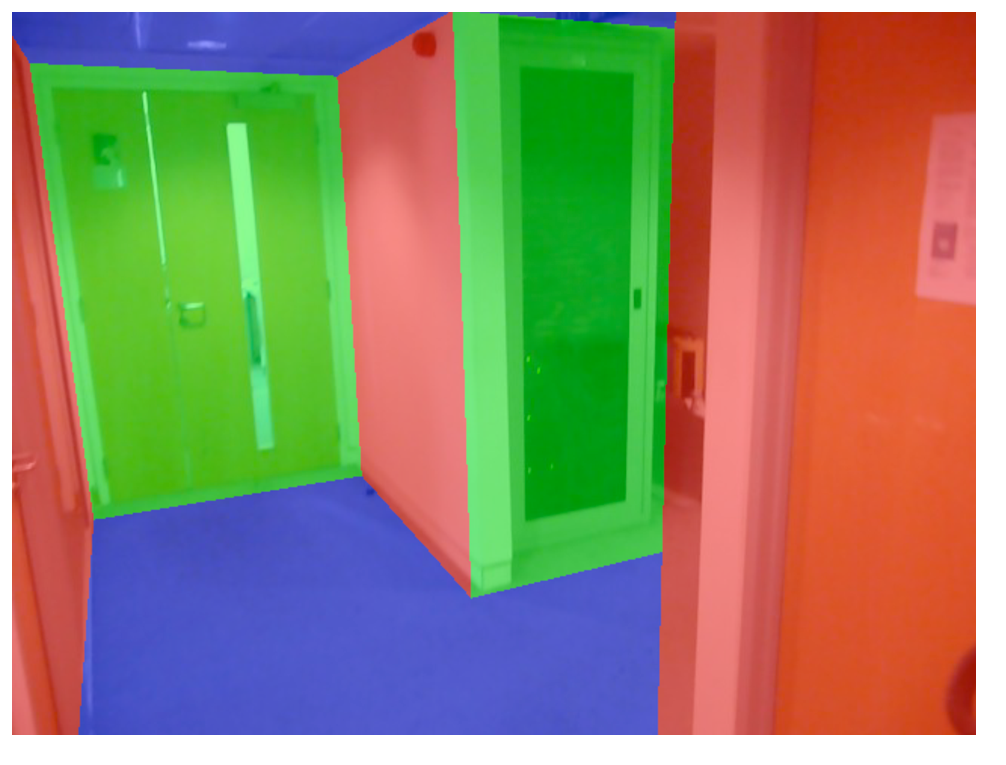
\includegraphics[width=0.5\textwidth]{manhattan-scene}
    \caption{An example of an indoor Manhattan scene.}
  \label{fig:manhattan-eg}
\end{figure}

In this thesis we present two approaches to deriving semantic--level
scene information from visual input. 

\subsection{Photometric Models}

The first model we present is a purely photometric approach and builds
on ideas from texture analysis, in particular the texton model. This
model associates each pixel with a discrete texture element, which is
then related to the semantic--level variable of interest. We show how
textons can be leveraged toward the problems of scene recognition and
contextual object search. Despite the simplicity of this approach, we
show that it is effective for the proposed problems.

In contrast to systems based on edges, interest points, or local
descriptors, utilising texture information allows us to leverage
visual information in non--salient image regions. This is particularly
important for environments in which there are few individually
distinctive image patches, yet the overall scene appearance conveys
significant information.

We present qualitative results motivating the use of texture structure
for the stated task, followed by a formal probabilistic model and
quantitative comparisons with the state--of--the--art.

\subsection{Coarse Geometric Models}

The second part of this thesis focuses on capturing geometric
information in a form well--suited to semantic--level reasoning. This
represents a departure from much of the scene understanding
literature, in which geometric information is captured implicitly,
rather than via explicit geometric assumptions. Our decision to work
with explicit geometric models is motivated by the observation that
much about scenes and objects is tied to the high--level shape of the
environment, particularly the location of major surfaces and
boundaries.

As a simple illustration of this, consider the image shown in
\figref{manhattan-eg}. Despite the low information content of the
image -- it is defined by just a handful of vertices -- a human can
make many high--level inferences about this environment, including
answers to questions such as (in order of increasing difficulty):
\begin{enumerate}
  \item{What is the direction of gravity?}
  \item{Where would doors most likely be found?}
  \item{Where would a person be most likely to stand and at what scale?}
  \item{Is this an office or a house?}
  \item{What is the absolute scale of the environment?}
\end{enumerate}

While the image does not provide enough information for definitive
answers to any of these questions, it does provide surprisingly strong
evidence given that it consists of just a few hundred bits of
information. Thus it seems that coarse geometric information is
particularly valuable for high--level inference.

The image in \figref{manhattan-eg} shows one example of an indoor
Manhattan environment \cite{Lee09}, which is the hypothesis class we
adopt for geometric reasoning in this thesis. Under this model the
world is composed of a floor plane, ceiling plane, and a set of
vertical walls that meet at vertical edges. Indoor manhattan
environments constitute a subset of the more general set of Manhattan
environments, in which any arrangement of surfaces in three dominant
directions is permitted. It is an attractive model for a number of
reasons. Firstly, as argued above, it captures geometric information
of high value for semantic--level reasoning. Secondly, despite the
strong geometric assumptions, a surprisingly broad range of
environments can be represented exactly or approximately as indoor
Manhattan models. Thirdly, strong geometric assumptions assist in the
interpretation of ambiguous image evidence, since salient information
in one region can constrain the interpretation of other
regions. Finally, an efficient inference algorithm exists for this
hypothesis class, which is the subject of later chapters.

There is no hard distinction between a ``geometry--less'' and a
``geometry--laden'' approach to scene understanding. In either case
one is drawing probabilistic inferences from images; the distinction
is in how those inputs are combined, which conditional independences
are assumed, and how the hypothesis class is formulated. Our choice to
incorporate geometry corresponds to a particular choice of
independence assumptions, which differ from those typically chosen in
photometrically inspired models. This thesis is concerned with the
recovery of geometry for the sake of the high--level inference that it
enables, not for the sake of the geometry itself, and our choice of
model reflects this.

\section{Exegesis}

The remainder of this thesis is organised as follows. Chapter 2
presents a review of literature relevant to this thesis. Due to the
connection of our work to the traditionally disparate fields of SLAM
and scene understanding, the literature review breaks down into scene
understanding work that has touched on geometry, and SLAM work that
has touched on scene understanding.

Chapter 3 presents an appearance--only approach to scene understanding
in the context of a moving camera. We work with textons as the basic
observation unit and present a probabilistic model connecting these to
scene categories and object locations.

We then begin the presentation of our work concerning indoor Manhattan
models. Chapter 4 presents the model formally, and covers various
geometric observations on which later chapters rest. There is little
prior work on the indoor Manhattan model, so we dedicate a full
chapter to defining the model formally and describing several useful
representations. We then turn in Chapter 5 to identifying the
orientation of three cardinal Manhattan directions given multiple
calibrated views. We show that estimating scene rotation jointly from
all available views is a dramatic improvement over the standard
approach of identifying vanishing points separately in each image. We
also show an order of magnitude improvement over approaches that use
surface normals estimated from a reconstructed point cloud.

Chapter 6 presents a probabilistic model relating sensor data to the
geometric quantities we wish to extract. We give separate
probabilistic models for photometric features, stereo data, and point
clouds, then we show how to combine these into a fully Bayesian model,
allowing our system to be easily tailored to a variety of contexts. We
present a dynamic programming algorithm that solves both
maximum--aposteriori and maximum--likelihood inference within our
model. This inference procedure is both fast and exact, making a
compelling alternative to previous approaches that explode
combinatorially in model complexity.

Chapter 7 presents a learning routine in which we learn to reconstruct
Manhattan environments based on training examples. We cast the
learning problem in a discriminative framework and use
state--of--the--art tools from the structured prediction
literature. We show that learning with respect to single versus
multiple views differs only by a change in feature space, and we
present extensive results for both contexts. 

Finally, chapter 8 summarises key results and suggests directions
for future work.


%%%%%%%%%%%%%%%%%%%%%%%%%%%%%%%%%%%%%%%%%%%%%%%%%%
%
\def\localpath{Review}
\graphicspath{{\localpath/figures/}}
\chapter{Literature Review}
\label{chap:review}
% If you like chapter abstracts ...
%\begin{quote}{\em This chapter describes an application of 

The abstract text is put into Ch\#/ab\#.tex, where
\# is the chapter number.
}\end{quote}
\section{Introduction}
In this section we provide a review of the literature relevant to this
thesis. We begin by examining the literature on context in
single--view computer vision. This area is of great interest since
many of the techniques may be transferable to our multiple--view
setting. We then turn to a review of the use of context in robotics
applications, a subject that has received somewhat sparse attention in
the literature and has, as yet, no cohesive formulation or problem
statement. 

%We close with a review of simultaneous localisation and
%mapping (SLAM) systems, which is relevant because the research
%presented in the remainder of this report involves reasoning processes
%that utilise SLAM systems to recover camera poses.

\section{Context in Computer Vision}
Over the past decade there has been renewed interest in the use of
contextual information for computer vision tasks. There are many
definitions of what ``context'' means and how to represent it. Here we
review the dominant paradigms that have emerged around contextual
reasoning in scene understanding. Many single--image contextual
approaches have been targeted at a specific problem --- namely that of
object recognition --- and while this is not aligned exactly with our
own goal it is still instructive to review these contributions because
the ideas they propose for inferring context are often separable from
the specific task to which the authors choose to apply them.

\subsection{Holistic Approaches}

\subsubsection{Gist Features}
The work of Torralba \etal \cite{Torralba03} has been very influential
in expounding the value of contextual reasoning for vision. In their
work, they compute a feature vector composed of statistics from the
entire image and use this to reason about the contents of the
image. This feature vector is termed the ``gist'' of the image and is
computed as follows. First, an input image is passed through a bank of
Gabor filters at $n$ orientations and $m$ scales, producing $nm$
response images. Next, each response image is divided into a $k \times
k$ grid. Finally the average over each grid cell is computed for each
response image, and these values are concatenated to form the final
feature vector of length $nmk^2$.

In early work, Torralba \etal used the gist vector to learn about
scene categories. They showed that images could be classified into
categories such as ``road'', ``forest'', and ``bedroom'' by applying a
support vector machine (explained below) directly to the gist
vector. In later work \cite{Torralba03} they show how the location and
scale of objects can be predicted from the gist vector. The
Expectation--Maximisation algorithm \cite{Dempster77} is employed
to learn a mixture of Gaussians that relates the gist features to the
probability of an object being present at various locations and
scales. An example prediction is shown in \figref{contextual-priming}.

Support vector machines (SVM) were proposed by Vapnik \cite{Vapnik95}
just over a decade ago and have since gained widespread support both
inside and outside the machine learning community. SVMs learn to
discriminate two classes by finding the separating hyperplane in
feature space for which the distance to training examples is
maximised.

The Expectation--Maximisation algorithm is a widely used tool for
parameter estimation in the presence of unobserved variables
\cite{Dempster77}. Direct inference in such cases would require
marginalisation over all unobserved variables, but the integrals
involved typically make this approach infeasible. The EM algorithm
overcomes this by iterating between two stages. First, the expected
likelihood is computed with respect to the unobserved variables (the
E--step), and second, the model parameters are maximised with respect
to the distribution computed in the first step (the M--step). These
steps are repeated until convergence.

\begin{figure}[tb]
\centering
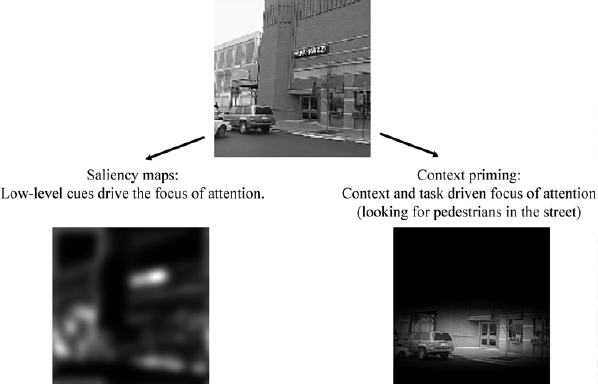
\includegraphics[width=0.75\textwidth]{contextual_priming.png}
\caption{Torralba \etal \cite{Torralba03} is able to improve upon
  traditional interest point detectors by learning the relationship
  between gist features and likely object locations. 
  \textit{Reprinted with express permission of Prof Antonio Torralba.}
  }
\label{fig:contextual-priming}
\end{figure}

\subsubsection{Scene Classification}

Fei--Fei and Perona \cite{Fei-fei05} classified images
explicitly into semantic categories such as ``coastal'', ``inner
city'', or ``bedroom''. Although their work focuses on the
classification task itself, the output scene label is clearly a useful
piece of contextual information for integration into a broader scene
understanding system.

Fei--Fei and Perona represent an image as a bag of words, where the
``words'' are obtained by clustering SIFT features (explained below)
obtained at regularly sampled locations across all training
images. Once the codebook of words has been learnt, each image is
collapsed to a simple sequence of integers representing the index of
the codebook entries identified within it.

Analogous to document understanding approaches in which each section
is associated with an inferred topic, Fei--Fei and Perona model a
hidden ``topic'' variable for each image feature. In their model they
also include a theme variable, which induces a class--conditional
multinomial distribution over topics.

On a dataset of 15 scene categories, each with several hundred images
taken from the web as well as from datasets released by other
researchers, the system obtains an average classification accuracy of
$64.0\%$.

The scale--invariant feature transform (SIFT) was first proposed by
Lowe \cite{Lowe99} for use in object recognition. Given some input
image, SIFT generates a set of interest points and corresponding
feature vectors that are robust to changes in lighting, scale, and
camera viewpoint. To select salient features at a range of scales, SIFT
builds a scale--space representation of the image \cite{Lindeberg93}
and selects locations that are well--localised in both the spatial and
scale dimensions. Features are generated from a histogram over
gradient orientations in a patch around each selected interest
point.

\begin{figure}[tb]
\centering
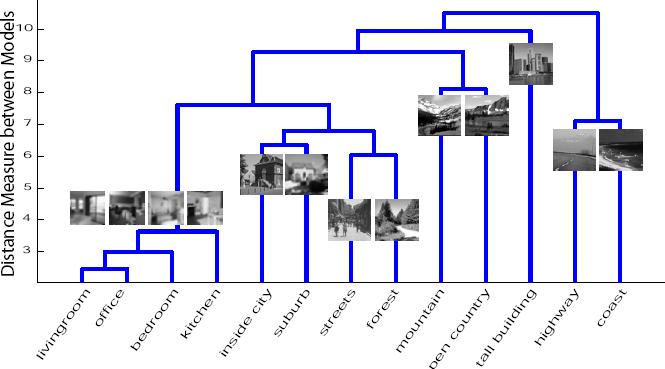
\includegraphics[width=\textwidth]{feifei_dendogram.png}
\caption{Dendogram showing the relationships between scene categories
  learnt by the system of Fei--Fei and Perona \cite{Fei-fei05}. The
  model matches human intuition well.
  \textit{Reprinted with express permission of Prof Fei--Fei Li.}
  }
\label{fig:dendogram}
\end{figure}

\subsection{Geometric Context}

An explicit understanding of scene geometry can assist image
understanding in numerous ways. Several authors have shown how to
obtain coarse 3D reconstructions from a single image, which allows
rich geometric reasoning for inference about such things as the
objects and actions likely to occur within the scene, and the scale
and position at which these might be found.

\subsubsection{Pixel--wise Geometry Estimates}

Hoiem \etal \cite{Hoiem06} approach geometric context as a per--pixel
labelling problem in which the labels identify geometric properties of
the 3D surface from which each pixel was captured. Although there are
many 3D scenes that could have generated any particular image, Hoiem
\etal note that some scenes are more probable than others given our
knowledge of the world. To keep this difficult inference task
tractable, the authors limit the pixel labels to ``sky'', ``ground'',
and ``vertical'', the last of which is further sub--divided into
``left--facing, ``right--facing'', and ``front--facing''. While there
are some real--world scenes that cannot be represented by these
geometric primitives, the authors show that they are able to model
many useful and interesting types of scenes.

The authors take a machine learning approach to the reconstruction
problem. First, the image is segmented into superpixels using the
algorithm of Felzenszwalb \etal \cite{Felzenszwalb04}. Next, pairs of
adjacent superpixels are merged in order to gradually grow the small
superpixels into larger regions. To do this, an affinity metric
between adjacent superpixels is learnt using a boosted decision tree
classifier, the input to which is a feature vector containing cues
such as colour, texture, location, shape, and vanishing points. At
evaluation time many different segmentations are generated by
considering the superpixels in different orders. For each ordering,
the first $k$ superpixels are assigned to unique segments, then the
remaining superpixels are assigned to the segment with which they have
the greatest affinity. Each segment is classified into one of the
geometric classes listed above using another a boosted decision tree
classifier with the same input cues as for the affinity metric
learning. Finally, superpixels are labelled according to the consensus
vote amongst the segments to which they belong.

The authors further show that the geometric labels obtained in this
way can be used as priors for object detection, since detections in
unlikely places and scales can be suppressed, while those in
geometrically consistent positions can be
amplified. \figref{hoiem-result} shows the improvement in detection
performance resulting from the use of geometric context.

\begin{figure}[tb]
\centering
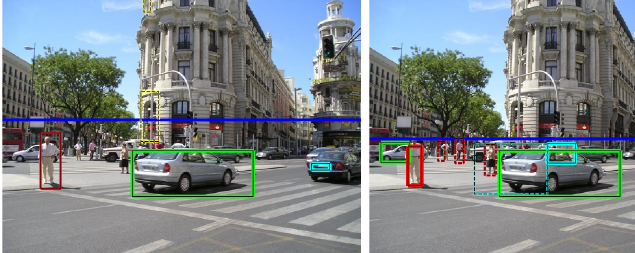
\includegraphics[width=\textwidth]{hoiem_detection_result.png}
\caption{The left image shows car and pedestrian detections when using
  local features only. The right image shows detections when geometric
  context is leveraged: several false--positives are eliminated and
  several new correct detections are made.
  \textit{Reprinted with express permission of Dr Derek Hoiem.}
  }
\label{fig:hoiem-result}
\end{figure}

\subsubsection{Make3D}

Another approach to deriving geometric context has been proposed by
Saxena \etal \cite{Saxena09}. Rather than the fixed set of
orientations employed by Hoiem \etal, Saxena \etal only assume that
the scene is piece--wise planar. They allow these planar patchlets to
take on arbitrary orientations, which they represent with a normal
vector.

Saxena \etal apply a machine learning methodology to this
problem. They begin by dividing the image into superpixels, each of
which is associated with a feature vector containing the output of a
set of filters, including colour, texture, and edges. Each superpixel
also includes the features of neighbouring superpixels so that the
inference process can reason in terms of broader image properties
rather than local statistics alone. In addition, each superpixel
boundary is associated with a separate set of features. These are
generated by running segmentations based on different image properties
and recording whether the boundary is present in each.

The superpixels are organised into a Markov Random Field (MRF), with
edges between pairs that share a boundary in the image. The node
potentials are learnt from the superpixel features and edge
potentials are learnt from the boundary features. The authors allow
for coplanar, connected, and disconnected relationships across
boundaries, with the former preferred \textit{a priori} over the
latter. The MRF parameters are learnt through Multi--Conditional
Learning and inference is performed by solving a linear program.

Within a dataset of 152 internet images the system was able to
generate a qualitatively correct model (as judged by a human) 64.9\%
of the time. One such result is illustrated in \figref{saxena-result}.

\begin{figure}[tb]
\centering
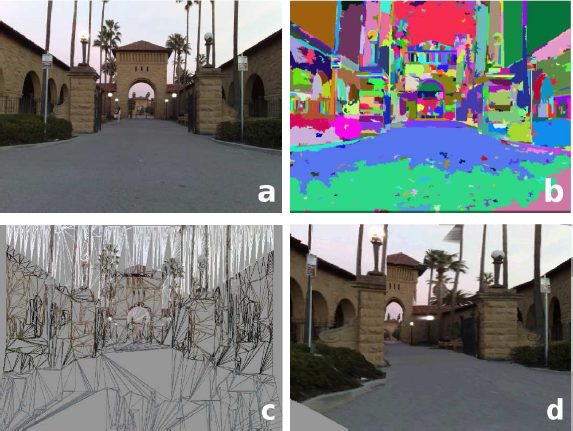
\includegraphics[width=0.5\textwidth]{saxena_results.png}
\caption{Results from the geometric context system of Saxena \etal
  \cite{Saxena09}. From top left to bottom right the panes show (a)
  the original, (b) the superpixels, (c) the inferred 3D model, (d) a
  re--projection of the 3D scene.
  \textit{Reprinted with express permission of Dr Ashutosh Saxena.}
  }
\label{fig:saxena-result}
\end{figure}

\subsection{Manhattan--World Approaches}

In recent years there has been growing interest in leveraging the
Manhattan world assumption, in which a scene is modelled using
surfaces oriented in three mutually orthogonal directions. This idea
was originally proposed by Coughland and Yuille \cite{Coughlan99}, who
were interested in recovering camera orientation from a single
image. It has since been used in a variety of tasks including
vanishing--point detection \cite{Zhang02}, single--view reconstruction
\cite{Lee09,Flint10eccv}, and multiple--view reconstruction
\cite{Furukawa09,Flint11}. In general, the Manhattan world assumption
is appealing for scene understanding tasks as it reduces the size of
the hypothesis class one must search over.

\subsubsection{Cuboid Models}

Hedau \etal \cite{Hedau09} reason about indoor environments by
modelling the scene as the interior of an axis--aligned cuboid. This
is perhaps the simplest possible instantiation of the indoor Manhattan
assumption, but the authors show that even this restrictive model can
be helpful when interpreting and recognising objects in photos of
indoor environments. Their approach proceeds in two stages. First,
three mutually orthogonal vanishing points are estimated from
observed line segments. Next, a cuboid is identified by casting two
rays from each vanishing point.

\changedsinceviva{
The authors use a structured prediction model to learn how to select
bounds for the cuboid. Given training examples they train an SVM to
rank cuboid hypotheses within a feature space defined over inputs
(image features) and outputs (cuboids). This approach
follows a similar methodology to the approach we propose in
\chapref{learning}, though we learn within a much more general
hypothesis class.
}

In later work \cite{Hedau2010} the authors connect the cuboid model of
spatial boundaries to a model of objects within the room. Objects are
modelled as axis--aligned cuboids resting on the floor. Several such
cuboids are hypothesised, and the support for each is determined by an
SVM trained with HOG features. The authors further show that by
reasoning jointly about room boundaries and the objects within, the
performance of both inference algorithms is improved.

\begin{figure}[tb]
  \centering
  \subfloat[Object hypotheses]{
    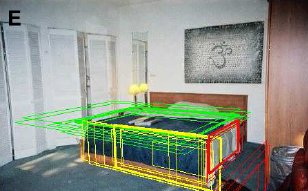
\includegraphics[width=0.35\textwidth]{hedau_a.png}
  }
  \subfloat[Scene layout and object boundary]{
    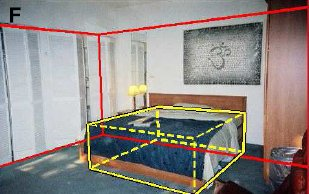
\includegraphics[width=0.35\textwidth]{hedau_b.png}
  }
  \caption{Results from the cuboid model of Hedau \etal
    \cite{Hedau09,Hedau2010}.
    \textit{Reprinted with express permission of Varsha Hedau.}
  }
  \label{fig:hedau-result}
\end{figure}

\subsubsection{Indoor Manhattan Scenes}

Lee \etal \cite{Lee09} have investigated geometric context for the
special case of \textit{indoor} Manhattan environments, which are a
sub--class of general Manhattan environments and have the following
properties:
\begin{itemize}
  \item{There is a floor plane and a ceiling plane, which are parallel
    to one another and extend indefinitely in all directions.}
  \item{There are planar wall sections, which are orthogonal to the
    floor, extend all the way from the floor to the ceiling, and
    terminate in vertical boundaries.}
  \item{The wall sections are oriented in one of two mutually
    orthogonal directions.}
  \item{Many objects within rooms are aligned with the floor and/or
    walls and hence there will be many edges sharing vanishing points
    with floor, walls, and ceiling.}
\end{itemize}

Although many real environments contain exceptions to these rules, the
authors argue that their model is expressive enough to represent
approximately or exactly many real--world scenes. This leads to a
particularly simple model in which scenes are represented by a ground
plane orientation and a set of wall segments.

Lee \etal show how such a model can be derived from a single
image. They begin by sampling two pairs of lines in a RANSAC--like
fashion to generate vanishing points. Each pair is checked for mutual
orthogonality (using a prior on camera focal length) and for support
amongst the other detected line segments. The intersection of the two
pairs gives two vanishing points, from which the third can be
derived. This results in a set of straight lines and their associated
vanishing points.

The authors show that, given the assumptions above, any set of lines
representing wall segments for which the associated vanishing points
are known either give rise to exactly one Manhattan world model or
violate a set of easily--checkable rules. They therefore proceed to
enumerate all valid hypotheses by running a branch--and--bound search
over all combinations of line segments. This remains tractable because
the validity check eliminates most combinations at an early stage of
branching. Of the valid hypotheses, they choose the one which is
maximally consistent with surface orientation estimates separately
inferred from the image. \figref{lee-result} shows some of the
building structures their system was able to infer.

The second half of this thesis is concerned with models in this
category.

\begin{figure}[tb]
  \centering
  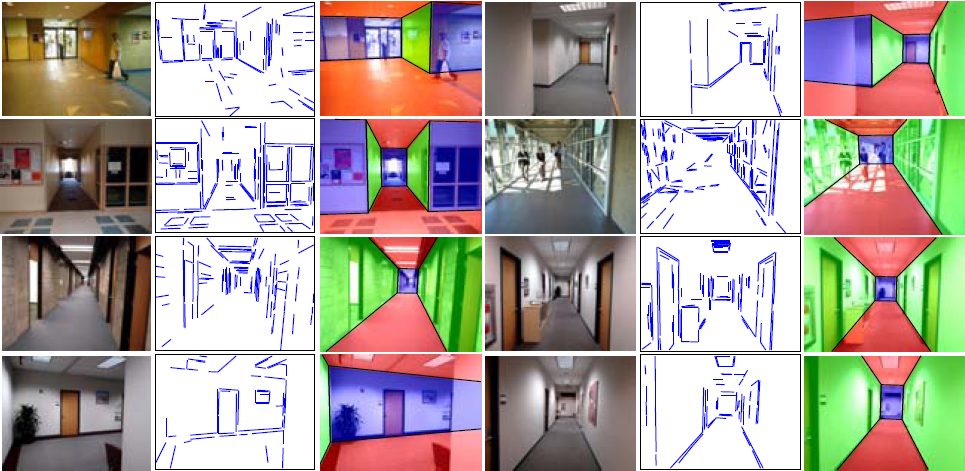
\includegraphics[width=\textwidth]{lee_result.png}
  \caption{Inferred scene structure obtained for single images by Lee
    \etal \cite{Lee09}. Each triplet shows the original image, the
    detected line segments, and the final scene geometry.
    \textit{Reprinted with express permission of David Lee.}
  }
  \label{fig:lee-result}
\end{figure}

\subsubsection{Oriented Plane Sweeps}

\changedsinceviva{
Gallup \etal \cite{Gallup2007} present a fast stereo algorithm based
on plane sweeping with respect to Manhattan--like surface
orientations. They proceed by (1) selecting a vertical direction based
on the camera trajectory; (2) identifying one horizontal and several
upright surface orientations based on lines and estimated vanishing
points; (3) performing plane sweep stereo with respect to each of
these orientations; and (4) fusing the result into a depth map. The
resulting depth map naturally encodes Manhattan scene structure since
each pixel is implicitly associated with one of the upright or
horizontal orientations.
}

\begin{figure}[tb]
  \centering
  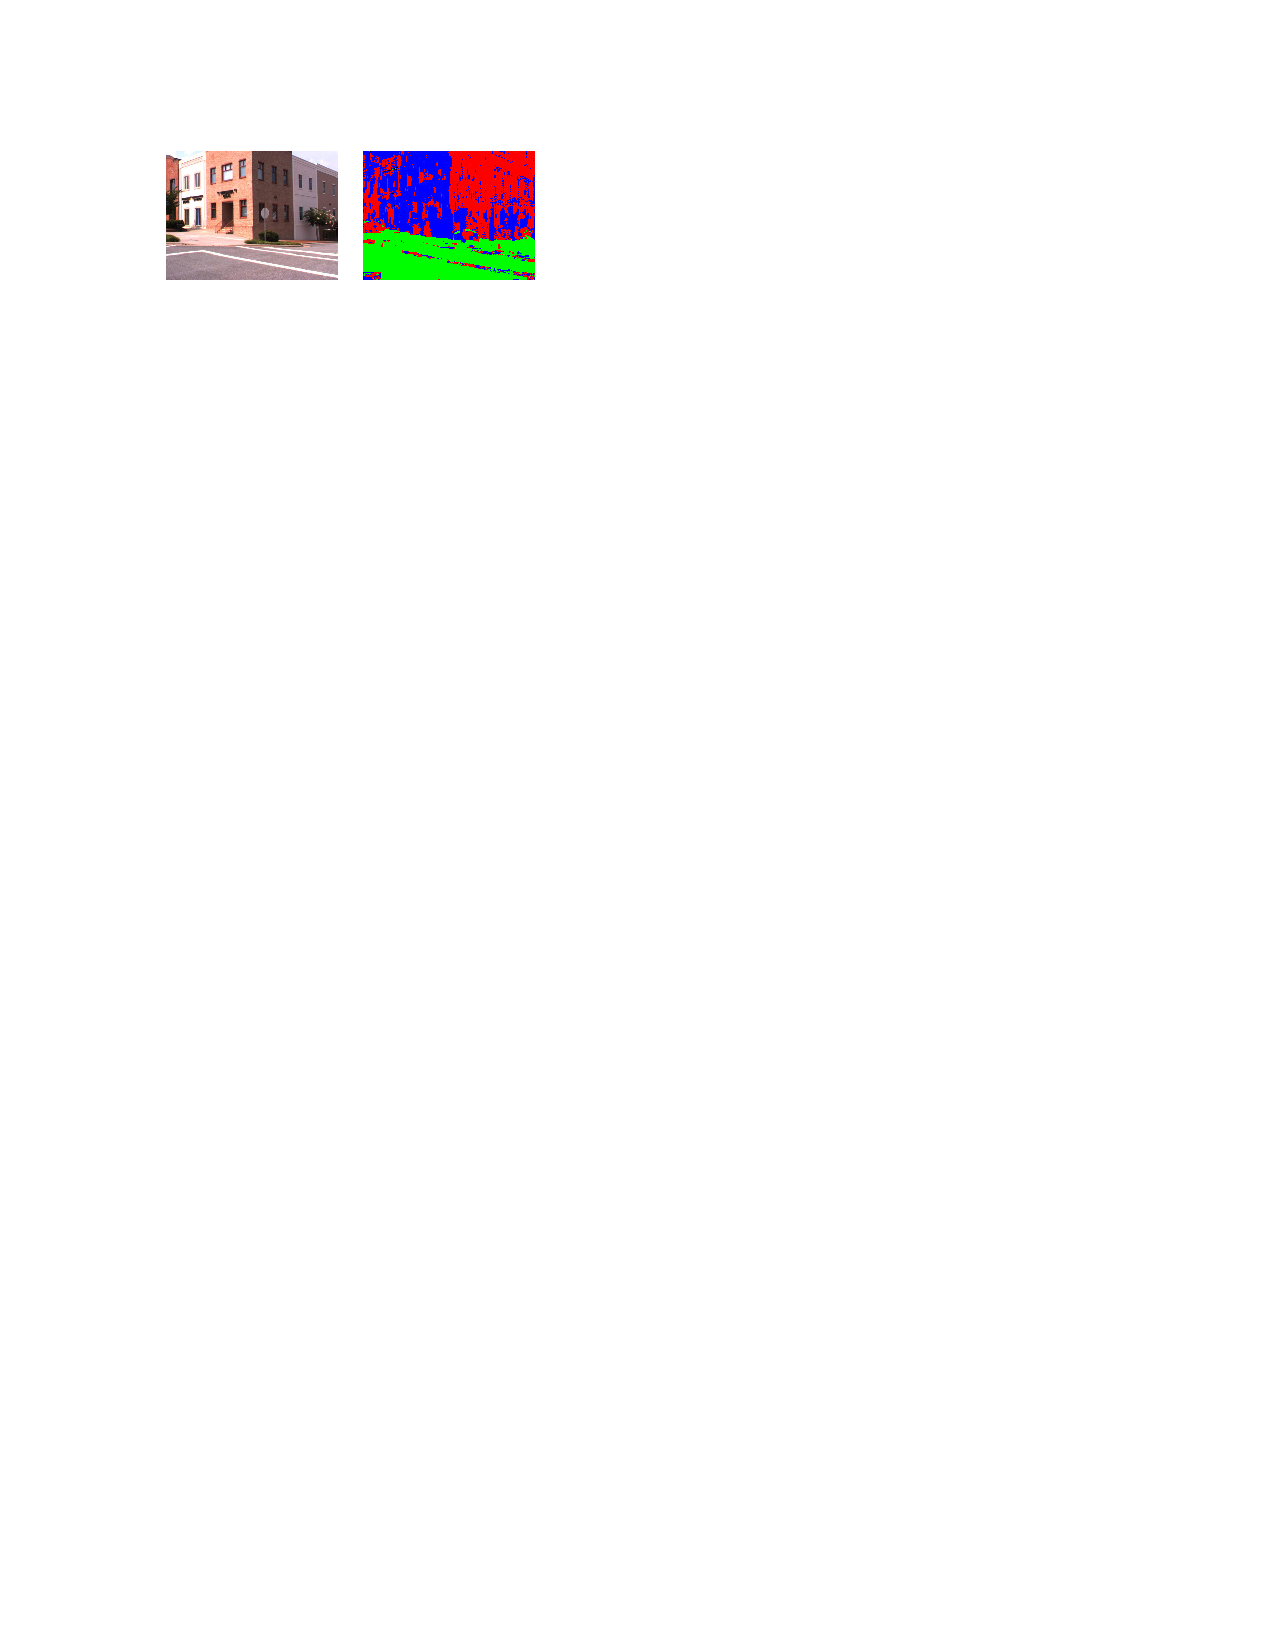
\includegraphics[width=0.6\textwidth]{gallup_result}
  \caption{Manhattan--like scene structure obtained from the
    multi--way plane sweep approach of Gallup
    \etal \cite{Gallup2007}.
    \textit{Reprinted with express permission of David Gallup.}
  }
  \label{fig:gallup-result}
\end{figure}

\subsubsection{Manhattan World Stereo}

Furukawa \etal \cite{Furukawa09} used the Manhattan world assumption
to improve the robustness of multiple--view reconstruction. Large
textureless surfaces are common within indoor environments --- for
example walls, ceilings, and floors. Such regions challenge many 3D
reconstruction techniques since identifying correspondences
between views is challenging. To overcome this, Furukawa \etal built a
3D reconstruction system that leverages the Manhattan world assumption
to extrapolate the layout of textureless regions from constraints
imposed by edges and corners, which are easier to localise in multiple
views. They model this task as an energy minimisation problem in which
each pixel must be labelled as belonging to some axis--aligned
plane. A smoothness prior ensures that system chooses the simplest
arrangement of planes that match the observed image evidence.

\subsubsection{Blocks World}

As early as 1965, Roberts \cite{Roberts65} proposed building scene
representations up from cuboid building blocks. This idea has recently
been revisited using modern probabilistic techniques by Gupta \etal
\cite{Gupta10}. Beginning with an empty ground plane, the authors
iteratively add cuboids to explain image features such as corners and
edges. Utilising a variety of stability and visibility constraints
the authors show that they are able to model a variety of scenes.

\begin{figure}[tb]
  \centering
  \subfloat[Input image]{
    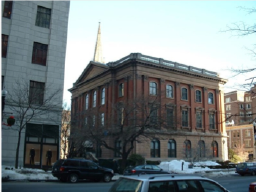
\includegraphics[width=0.3\textwidth]{gupta_a.png}
  }
  \subfloat[Inferred scene structure]{
    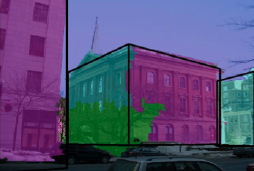
\includegraphics[width=0.3\textwidth]{gupta_b.png}
  }
  \subfloat[3D rendering]{
    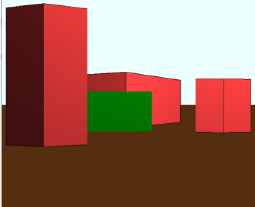
\includegraphics[width=0.3\textwidth]{gupta_c.png}
  }
  \caption{Results from the blocks world model of Gupta \etal
    \cite{Gupta10}.
    \textit{Reprinted with express permission of Dr Abhinav Gupta.}
  }
  \label{fig:gupta-result}
\end{figure}

\subsubsection{Vertical Structure Priors}

\changedsinceviva{
Zeisl \etal \cite{Zeisl2011} improve upon traditional stereo
algorithms by constraining reconstructions to a pair of horizontal
planes (floor and ceiling) spanned by arbitrary vertical
surfaces. Similarly to the algorithm we present in
\chapref{inference}, they use dynamic programming for exact inference
within their model. One difference between their approach and the one
taken herein is that they permit arbitrary vertical surfaces, not just
manhattan--oriented planes, and they penalise overall model complexity
in a different way. We discuss the connection between this approach
and our own, and given an empirical comparison in
\chapref{inference}. 
}

\subsubsection{Horizontal/upright Models}

Delage \etal \cite{Delage2006} presented early single--view
reconstruction work that focussed on identifying the boundary between
horizontal and upright surfaces. They modelled this floor/wall
fracture as a dynamic Bayesian network over image pixels, for which
efficient dynamic programming inference algorithms are well known.

Barinova \etal \cite{Barinova08} adopt a Manhattan--like hypothesis
class for outdoor scenes. Their models consist of a ground plane
supporting a series of vertical facades, which they infer using a
conditional random field over pixels. The key inference problem in
their approach is to recover a polyline separating the ground plane
from the series of vertical facades. They use a standard
Expectation--Maximization algorithm for maximum--likelihood inference,
and component--wise logistic regression to learn the CRF parameters
from training data.

Felzenszwalb and Veksler \cite{Felzenszwalb10} discuss a class of
dynamic programming algorithms capable of maximum--likelihood
image segmentation under various shape priors. One of the applications
to which they apply their algorithm is single--image reconstruction.

Common to each of these approaches is a model that decompose into
vertical segments running from left to right in the image. We take
advantage of a similar decomposability within indoor Manhattan
environments in the inference algorithm that we propose in
\chapref{inference}.

\subsubsection{3D stages}

\changedsinceviva{
Nedovic \etal \cite{Nedovic2010} derive geometric context by
classifying images into 15 ``stage categories''. Each category
consists of an arrangement of surfaces such as ``ground'', ``sky'',
``upright'', ``background'', and ``figure'', such as those shown in
\figref{nedovic-stages}. Their principal contribution is a large
selection of powerful visual features containing salient geometric
information, including cues derived from color, shape, texture
gradients, atmospheric scattering, line segments, and segmentation
boundaries. The authors train an SVM to associate input images with
one of the 15 stage categories.
}

\changedsinceviva{
Their work relates to ours as follows. 13 of the 15 proposed stages
are special cases of indoor Manhattan environments, which we analyse
extensively in this thesis. The remaining two include an upright
``person'' segment, which we do not consider. The learning scheme we
propose in \chapref{learning} is also based upon large margin
principles, but whereas Nedovic \etal learn with respect to 15
categories, we learn with respect to the much larger space of all
possible indoor Manhattan models. The features they propose seem well
suited to our own purposes and so future work could apply our
inference and learning strategies to their features.
}

\begin{figure}[tb]
  \centering
  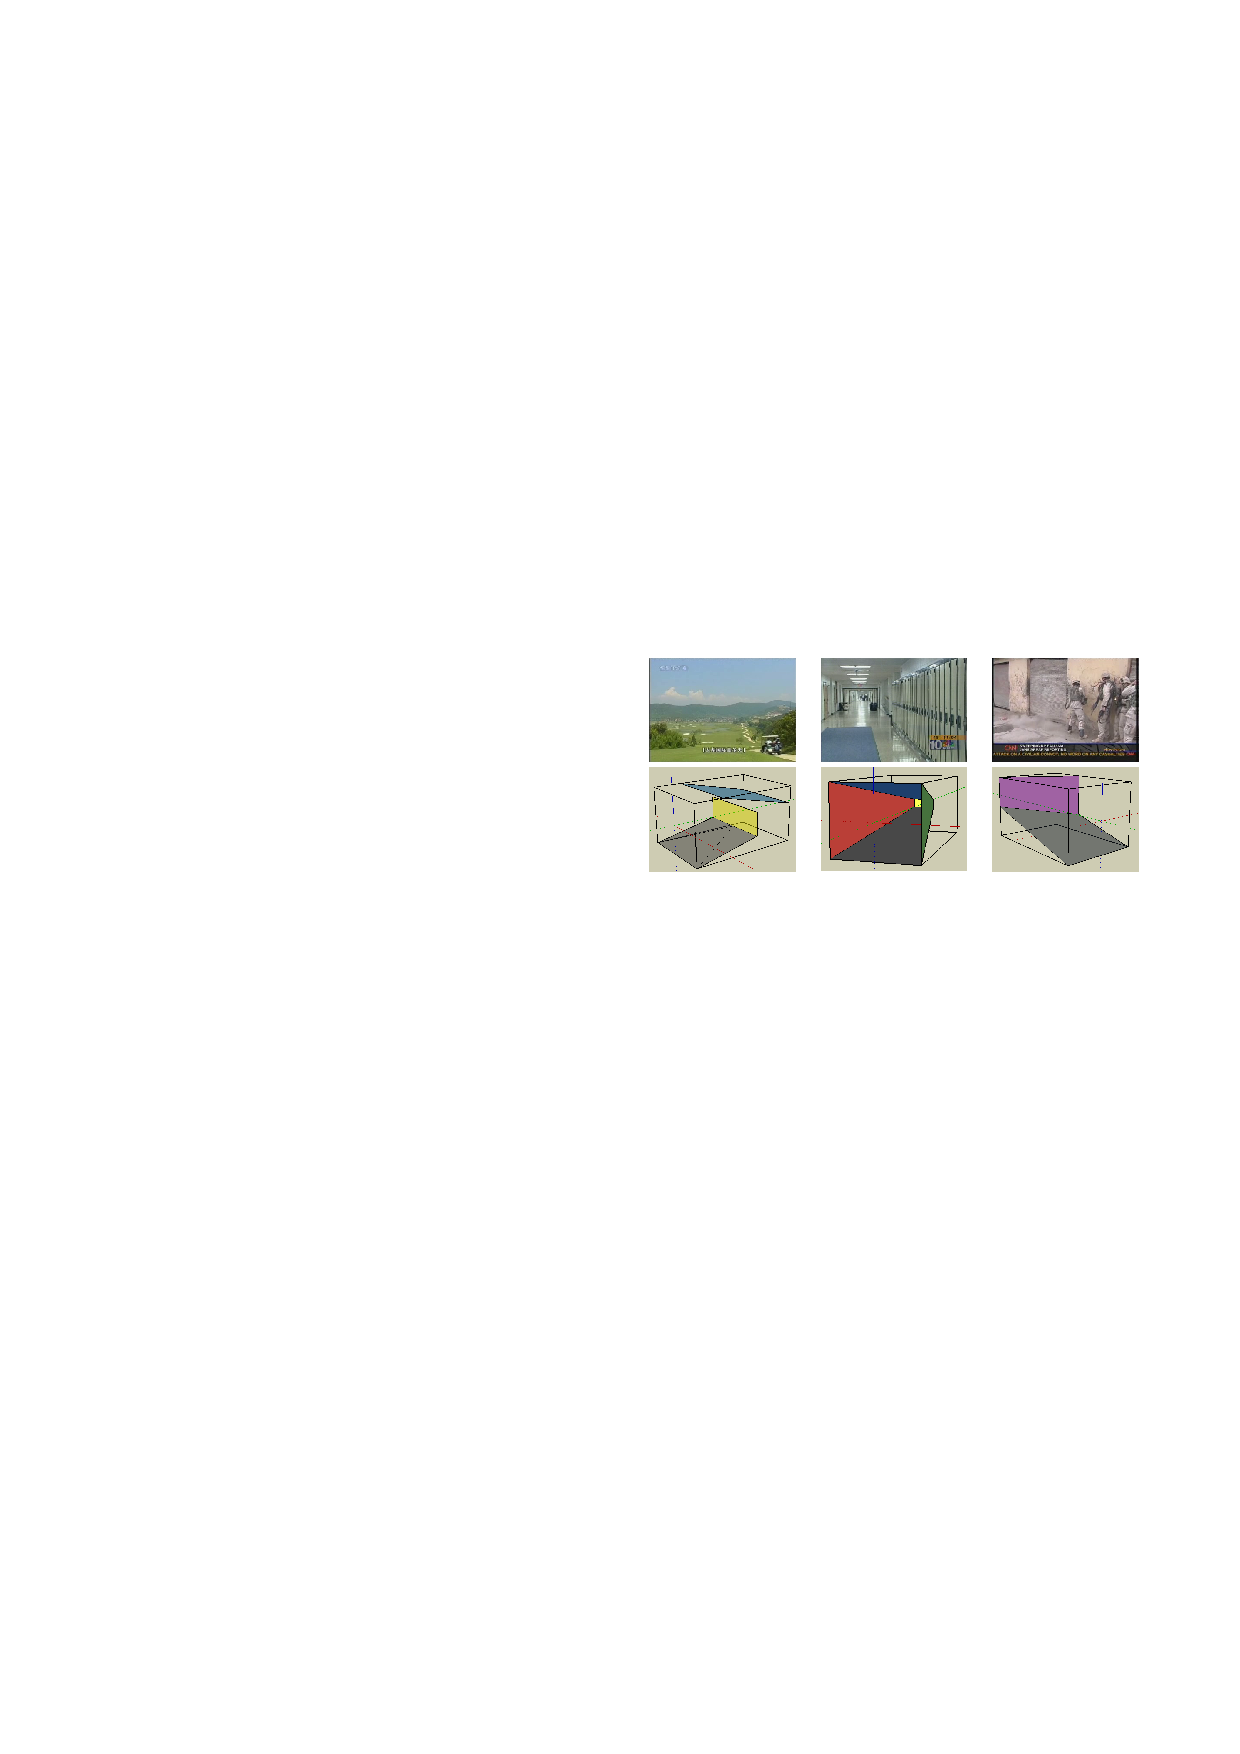
\includegraphics[width=0.75\textwidth]{nedovic_stages}
  \caption{Three categories of ``3D stages'' defined by Nedovic \etal
    \cite{Nedovic2010}, with examples of representative images.
    \textit{Reprinted with express permission of Vladimir Nedovic.}}
  \label{fig:nedovic-stages}
\end{figure}

\subsection{Texture Recognition}

Heitz and Koller \cite{Heitz08} derived context from texture structure
in images. Their model relates the presence of objects, which have
specific boundaries, to the appearance of the nearby surfaces and
foliage, which have no crisp notion of spatial support. This approach
is motivated by the observation that object positions correlate with
the appearance of their surroundings. For example, cars and bikes are
likely to appear near road--like texture, whereas aeroplanes are
likely to appear against a sky--like background.

\changedsinceviva{They begin by identifying superpixels using the
  segmentation algorithm described by Ren and Malik \cite{Ren03},
  which is extends the normalised cuts algorithm due to Shi and Malik
  \cite{Shi2000} }. Each such region is associated with a feature
vector comprising various colour and texture statistics, which, in
their model, arises from a latent category variable, the intention
being that superpixels will be clustered into meaningful groups like
``road'' and ``sky''. Meanwhile, a set of candidate object detections
is generated by invoking a standard object detector and taking all
detections above a certain threshold. The ``things'' are related to
the ``stuff'' by a set of observed variables representing spatial
relationships such as ``above'', ``beneath'', and ``next to''.

An advantage of the this model is that while object labels are
required for training, no explicit segmentations or labels are
required for the system to learn how to categorise the ``stuff''
regions since the system is capable of learning these
unsupervised. The authors achieve this using the EM algorithm, which
iterates between estimating the superpixel labels and optimising the
appearance parameters for each label.

The authors also show how to learn a set of relationships that best
describe the dependencies between objects and their surroundings. This
involves augmenting the EM algorithm with a greedy search over
possible relationships, iteratively adding the best candidate out of a
pre--defined pool until convergence. This allows the system to adapt
to the most salient relationships for a specific problem, which will
differ between, say, images captured from satellites and the photos in
the VOC datasets \cite{VOC2009}. During evaluation both the object
labels and superpixel labels are unknown, so exact inference is
intractable. Instead, the authors use an approximate inference
technique called Gibbs sampling.  \figref{TAS-regions} shows some
example superpixel clusters along with their probabilistic
relationship to car detections.

\begin{figure}[tb]
  \centering
  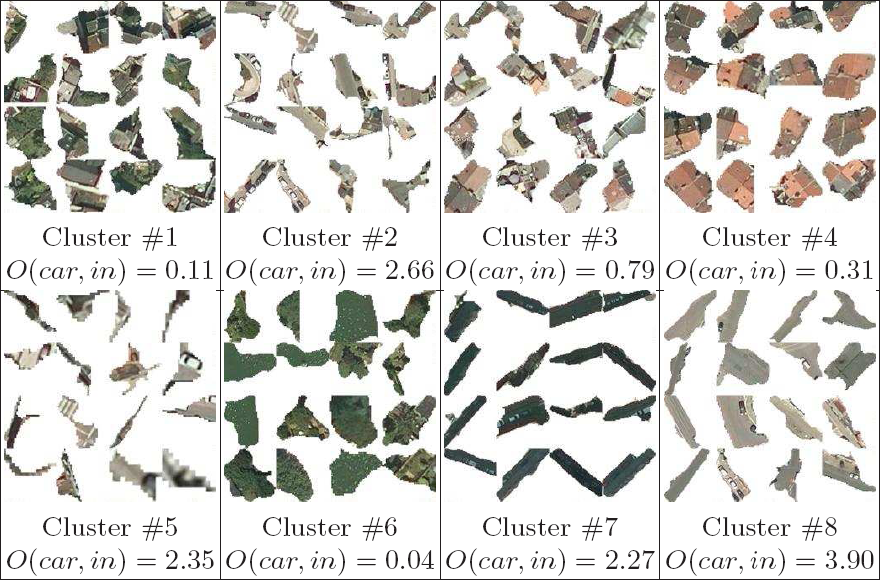
\includegraphics[width=0.75\textwidth]{TAS_regions.png}
  \caption{Superpixels clusters generated by the model of Heitz and
    Koller \cite{Heitz08}. Shown below each panel is the odds ratios for
    a car appearing near a superpixel from that class. The odds ratio is
    higher for road--like regions than for foliage-- or water--like
    regions.
    \textit{Reprinted with express permission of Prof Daphne Koller.}
    }
  \label{fig:TAS-regions}
\end{figure}

\section{Context in Robotics}
Cameras have long been recognised as a valuable sensor for mobile
robotics. In addition to visual SLAM, cameras have been used in
robotics tasks such as place recognition \cite{Cummins08} and scene
description \cite{Posner08}. Contextual reasoning has received little
attention from the robotics community. This section reviews the
literature that does exist on this topic. We divide the work into two
categories: map--centric approaches, which integrate sensor data into
a map and then reason from this representation, and ego--centric
approaches, which organise sensor data as a time--indexed series of
observations.

\subsection{Ego--centric approaches}
Martinez \etal \cite{Mozos05} have demonstrated that a robot can learn
to classify its environment into semantic categories such as
``corridor'' or ``room'' based on simple range data features. They
employ a SICK laser, which gives a $360\degrees$ scan of the scene
within a single horizontal plane. They collect features such as the
distance between successive beams, the average beam length, and the
eigenvalues of the polygon formed by the beam endpoints, which are
concatenated to form a feature vector at each time step.

To relate these features to semantic categories, the authors employ
the AdaBoost algorithm \cite{Schapire98} using linear classifiers as
the weak learners. AdaBoost is a popular classifier that learns by
incrementally adding rules that maximally correct the mistakes it has
made so far. Martinez \etal show that they are able to differentiate
rooms, corridors, and doorways at 89\% accuracy using this
method. Furthermore, in environments that have not been seen before
the system obtains 82\% accuracy. The results for one environment are
depicted in \figref{martinez-result}.

\begin{figure}[tb]
  \centering
  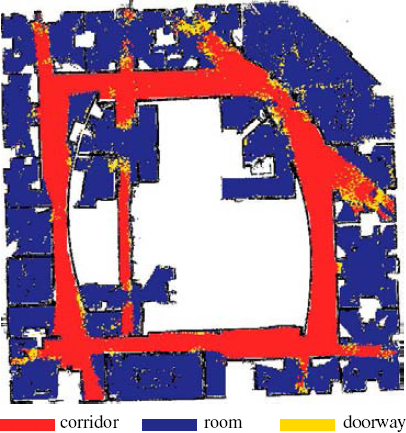
\includegraphics[width=0.5\textwidth]{martinez_result.png}
  \caption{Semantic labels assigned by the range data classification
    system of Martinez \etal \cite{Mozos05}. 82\% of places were
    correctly classified, despite the environment not having been seen
    during training.
    \textit{Reprinted with express permission of Dr Oscar Martinez Mozos.}
    }
  \label{fig:martinez-result}
\end{figure}

Stachniss \etal \cite{Stachniss05} extends this to use visual cues
from a panoramic camera in addition to the laser range data. Stachniss
runs an off--the--shelf object detector for each of several object
categories that correlate well with location. The chosen objects
include computer monitors, coffee machines, and soap dispensers. At
each time step, the robot's current location is categorised using the
same AdaBoost classifier as described above, the only difference being
that now the number of visual detections of each object type are
appended to the AdaBoost input vector. This allows the classifier to
select between visual and range data features (or combinations
thereof) according to whichever is most salient for the task at hand.

The authors recognise that the robot's location is highly correlated
over successive time steps and so model the robot's state as a Hidden
Markov Model (HMM), with the transition probabilities estimated
empirically. Stachniss \etal show that the addition of visual cues
allow them to differentiate between rooms with a similar shape but
different visual appearance (such as bedrooms and living rooms),
whereas the original range--data--only approach of Martinez would fail
in this case.

Posner \etal \cite{Posner08} show how to learn semantic labels such as
``grass'', ``foliage'', or ``wall'' for regions within urban
environments. Like the systems described above, they reason from a
combination of laser and vision features, including colour, location,
and orientation properties. Unlike previous approaches they perform a
quantisation step to form feature ``words''.

Incoming images are segmented based jointly on an off--the--shelf
superpixel algorithm and continuity boundaries in the laser data,
after which the problem is reduced to determining the appropriate
label for each segment. They relate the features for each region to
semantic labels using a graphical model that incorporates observation
likelihoods as well as a sensor model describing the probability of
false positive and false negative observations. While a standard
approach would be to assume independence between the feature
observations for tractability, the authors note that the observations
are far from independent in reality and instead employ the Chow Liu
algorithm to find the best tree--structured approximation to the full
joint distribution. Inference within this model is performed by
computing the full posterior over labels.

Posner \etal further refine the labelling by relating the labels of
neighbouring patches in an MRF framework. They introduce edges for
both spatial and temporal consistency, the former being derived from
adjacency between segments within the image, and the latter being
derived by reprojecting laser points into consecutive frames. Node
potentials are given by the segment classifier described above
while edge potentials are learned empirically from hand--labelled
training data. Sequential tree--reweighted message passing (TRW--S) is
chosen for inference within the MRF due to its efficiency guarantees.

The authors show that their system is able to accurately label a range
of outdoor environments with 8 categories (grass, tarmac, dirt path,
textured wall, smooth wall, foliage, vehicle). Their classifier
obtains the highest precision for the ``grass'' category ($95.5\%$)
and the lowest for ``vehicles'' ($79.7\%$). Furthermore, their system
is able to run in under 4 seconds, which is suitable for periodic
on--line operation. An example labelling is illustrated in
\figref{posner-result}.

\begin{figure}[tb]
  \centering
  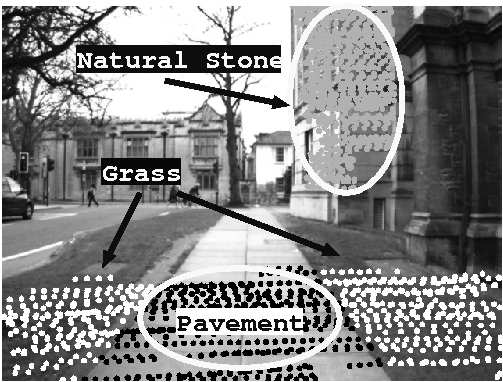
\includegraphics[width=0.6\textwidth]{posner_result.png}
  \caption{Semantic labels output by the system of Posner et al
    \cite{Posner08}.
    \textit{Reprinted with express permission of Dr Ingmar Posner.}
  }
  \label{fig:posner-result}
\end{figure}

\subsection{Map--centric approaches}
An alternative approach to deriving context in robotics applications is
to integrate new measurements into a map, and then reason about
semantics within the map representation. In general this approach
enables stronger integration of measurements taken over several time
steps, at the cost of relying on the ability to correctly build a map.

Buschka and Saffiotti \cite{Buschka02} have taken a map--centric
approach to the problem of identifying room boundaries within indoor
environments and recognising the resultant rooms. A series of laser
range scans are fused into a 2D occupancy grid representing the
probability that each cell is occupied by some object or
boundary. Rooms boundaries are identified by applying dilation and
erosion to the occupancy map, which are standard morphological filters
from visual segmentation \cite{Forsyth02}. The
authors demonstrate that this can be performed with fixed
computational cost by discarding old parts of the environment as the
robot moves through the environment.

The result of their algorithm is a series of ``nodes'' with topological
connections between them, which correspond to the various rooms and
corridors within the robot's environment and the doorways that connect
them. The authors proceed to characterise each node by the size and
eccentricity (length to breadth ratio) of its bounding box. This gives
contextual information in two senses: firstly, the identification of
room boundaries allows reasoning in terms of rooms rather than the
entire known environment, and secondly, the characterisation of room
shapes allows differentiation between rooms and corridors and thus
allows different interpretations of sensor data in these semantically
distinct workspaces.

Vasudevan \etal \cite{Vasudevan07} use an alternative map representation
based around the location of objects. They argue that this matches
human perception of space. In their maps, each ``object'' (actually a
SIFT landmark) occupies a separate coordinate frame, with uncertainty
represented in the transformations between frames.

They identify doorways by running a line detector and testing various
combinations of lines against a set of heuristics, enabling separation
of the constituent rooms within an environment. This in turn allows
per--room reasoning as was the case with the Buschka and Saffiotti
system described above. The difference here is that Vasudevan \etal
identify doorways directly from visual input whereas Buschka and
Saffiotti use occupancy maps.

Vasudevan \etal show that this representation leads naturally to
reasoning about place context. They argue that place categories
(bedrooms, kitchens, bathrooms, \etc) can be identified by the objects
within them, and hence that their object--centric maps provide the
perfect setting for this form of contextual reasoning. Formally, they
learn a class--conditional object likelihood by computing the number
of times each object is observed in each type of places versus the
total number of times the place category has been observed. They then
assume independence between object observations and compute the
posterior over place categories by multiplying out the likelihoods for
each observed object. 




%% \section{SLAM}
%% In order for a robot to navigate within an unknown environment it must
%% build a map of its environment and simultaneously localise itself
%% within that map. The representation of the map and robot pose, and the
%% techniques used to estimate these quantities, form the problem known
%% as simultaneous localisation and mapping (SLAM). These problems are
%% difficult because the solution to either part seems to rely upon the
%% solution to the other, yet it is also a problem of great importance,
%% since a working SLAM system is a first requirement for many robotics
%% and vision tasks, such as navigation, path planning, spatial
%% reasoning, and augmented reality.

%% Despite the considerable progress of SLAM systems over the past two
%% decades, implementations remain imperfect and cannot be treated as
%% infallible black boxes. However, our work is intended to
%% \textit{utilise} SLAM rather than improve upon the state--of--the--art
%% so we keep this section brief, simply outlining the major paradigms
%% within the literature.

%% \subsection{Bundle Adjustment}

%% The SLAM problem can be modelled as a maximum--likelihood inference
%% problem over robot pose and landmark locations. The standard
%% probabilistic model for SLAM consists of a sequence of poses
%% $\vect{s_t}$ organised as a Markov chain, a set of landmark locations
%% $\vect{x_i}$, and at each time step, and a set of landmark
%% observations $\vect{z_j}$ connecting landmarks and poses. Assuming
%% Gaussian observation errors, maximum likelihood inference can be
%% written as a nonlinear least squares optimisation problem known as
%% bundle adjustment. This is in fact the standard approach to the
%% offline variant of SLAM known as structure--from--motion, but for
%% online applications, full bundle adjustment is too expensive in both
%% time and space. Each SLAM algorithm described below can be viewed as a
%% particular approximation to the full maximum likelihood solution.

%% \subsection{Kalman Filtering}
%% The Kalman filter \cite{Kalman60} is a recursive state estimator that
%% represents the posterior over states as a Gaussian distribution. The
%% Extended Kalman Filter (EKF) generalizes this approach to non--linear
%% observation models, which was applied to SLAM by Smith and Cheeseman
%% \cite{Smith87}. 

%% The relationship between the EKF and the maximum likelihood approach
%% is as follows. If the posterior on states is a Gaussian distribution
%% and the observation model is linear then the EKF is the maximum
%% likelihood estimator. Unfortunately, the state vector in SLAM includes
%% entries for all landmarks as well as the robot pose, and in reality
%% the posterior over these quantities is highly
%% non--Gaussian. Another drawback of the EKF is the necessity of
%% maintaining a full covariance matrix over the system state, which in
%% the case of SLAM grows with the number of landmarks.

%% \subsection{Particle Filtering}
%% Particle filters are a class of recursive state estimator that
%% approximate the posterior over states by sampling from it. At the
%% first time step, a series of samples are drawn from the prior over
%% states, then at each time step samples are updated according to new
%% observations. There are several methods used to perform this update;
%% for example, the Sequential Importance Resampling algorithm of Gordon
%% \etal \cite{Gordon} propagates samples through a proposal
%% distribution, then assigns weights to each sample by evaluating the
%% posterior. Over time, samples in low--probability regions of the
%% distribution are deleted and replaced by cloning samples in
%% high--probability regions.

%% \subsection{Parallel Tracking and Mapping}
%% Klein and Murray \cite{Klein07} developed an approach to SLAM in which
%% the posterior over states is approximated by applying bundle
%% adjustment to a sample of frames from the input sequence. Their
%% system, known as parallel tracking and mapping (PTAM), uses bundle
%% adjustment to resolve the 3D locations of a set of landmarks, which
%% are then tracked through the remainder of the video stream. During the
%% tracking phase, landmarks are considered fixed, so only the camera
%% pose is being estimated. When necessary, an incoming frame is selected
%% as a new key--frame, which adds a new set of landmarks to the map. The
%% bundle adjuster then updates the position of all landmarks and camera
%% poses in a separate thread, while the landmarks continue to be tracked
%% in real--time. This allows the system to maintain an up--to--date
%% estimate of the camera position without conceding any of the
%% approximations involved with Kalman filtering or particle filtering.

%% PTAM possesses a number of advantages over other SLAM systems. First,
%% the division of tracking and mapping into separate threads allows PTAM
%% to maintain very dense maps (thousands of points), which would be
%% intractable for real--time performance under other SLAM paradigms.
%% Second, PTAM gains robustness to measurement errors because frames
%% containing low--quality observations will not be selected as
%% key--frames. PTAM also gains robustness from the large number of
%% landmarks it tracks, which allows a robust estimator to reliably find
%% inliers even in the face of many outliers. For these reasons we use
%% PTAM throughout the experiments in this thesis, though all of our work
%% could equally well utilise any other SLAM system.

%% \begin{figure}[tb]
%%   \centering
%%   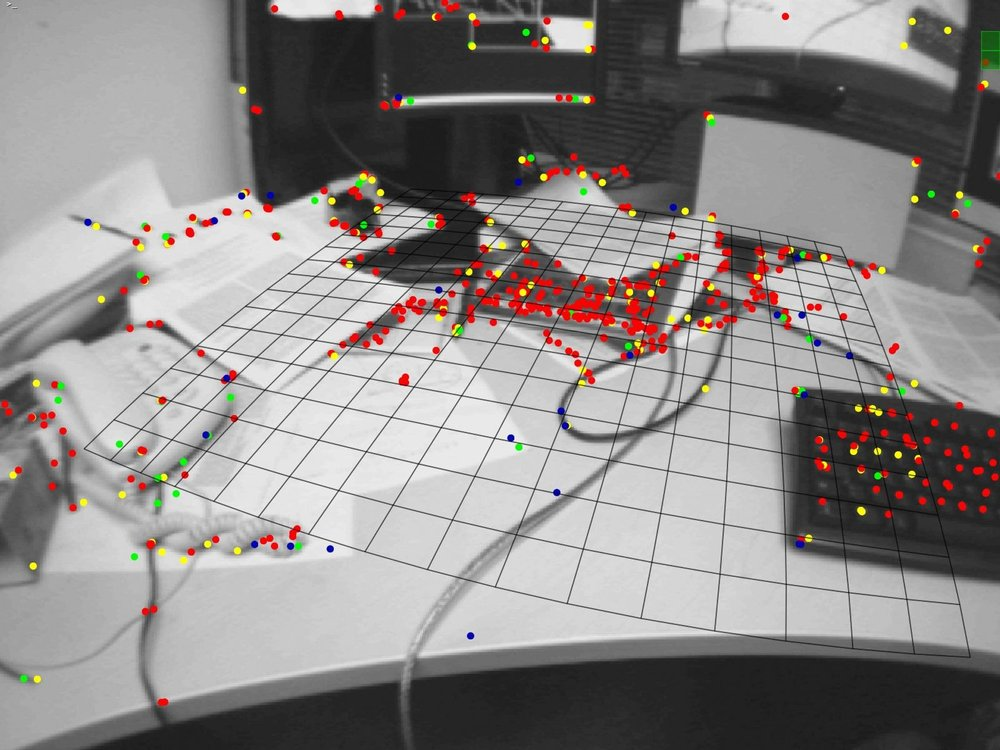
\includegraphics[width=0.6\textwidth]{klein_result.jpg}
%%   \caption{A set of key--points identified by PTAM
%%     \cite{Klein07}.
%%     \textit{Reprinted with express permission of Dr Georg Klein.}
%%   }
%% \label{fig:klein-result}
%% \end{figure}


\section{Conclusions}
Modern structure--from--motion systems generate accurate metric maps
of an environment, and can do so robustly and efficiently using visual
input alone \cite{Klein07}. The problem of deriving high--level
semantic context from such sensor data has been approached by several
authors. Although there is not yet a widely agreed--upon problem
formulation, current work in this area shows that semantics are
important for many robotics applications, and can be derived from a
range of sensor types. Important contributions include that of
Martinez \cite{Mozos05} and Stachniss \cite{Stachniss05}, who show
that place categories can be obtained from photometric and geometric
cues, and Posner \cite{Posner08}, who shows that scene regions can be
associated with semantic categories, again by combining vision and
range sensors.

The contextual reasoning problem for single--image vision has received
comparatively greater attention. Torralba's seminal gist descriptor
\cite{Torralba03} has led to the development of many types of
contextual cues, including geometric \cite{Hoiem05,Saxena09}, textural
\cite{Heitz08}, and model--based \cite{Lee09} approaches. Our work is
motivated largely by the success of the single--image approaches
discussed above; in this thesis we show how to extend these ideas to
incorporate a moving camera and the geometric information that a SLAM
system provides.



%%%%%%%%%%%%%%%%%%%%%%%%%%%%%%%%%%%%%%%%%%%%%%%%%%
%
\def\localpath{AppearanceOnly}
\graphicspath{{\localpath/figures/}}
\chapter{Appearance--Only Context Models}
\label{chap:appearance-only}
% If you like chapter abstracts ...
%\begin{quote}{\em This chapter describes an application of 

The abstract text is put into Ch\#/ab\#.tex, where
\# is the chapter number.
}\end{quote}
\begin{quote}
  This chapter explores an approach to scene understanding that
  relates low--level image information directly to high--level
  variables describing scene categories and coarse geometry. We
  build on a well--known texture analysis approach in which pixels are
  identified with characteristic texture units known as
  textons. Extending previous work in texture analysis and image
  recognition, we show that this approach --- which has previously been
  applied to recognition of uniform textures --- extends to 
  high--level scene understanding problem in which the input image is
  composed of many objects and surfaces. We propose a novel
  recognition model in which we measure the displacement between
  texton occurrences in an image rather than their absolute location
  or overall frequency. We apply our ideas to two classification
  tasks: place recognition and camera orientation
  classification. Comparisons with the gist descriptor of Torralba
  \etal show superior performance on both tasks.\footnotemark
\end{quote}

\footnotetext{This work was published in part in:

{ \setlength{\parindent}{0pt} 
  \textit{Flint, Murray, and Reid,} ``Learning Textons For
  Real--Time Scene Context'', in \textit{Proceedings of the
    First International Workshop on Ego--Centric Vision, 2009}\cite{Flint09}
} 
}

\section{Introduction}
One important aspect of scene understanding is the ability to
differentiate between logical areas within an environment, such as
rooms in a house. This problem is important in the domain of augmented
reality because knowledge of the location of a user will give a strong
indication as to the activities the user might undertake and the
objects with which they are likely to interact. 

Outside this specific application area, place recognition can be used
as a generic source of context for further scene understanding
tasks. Object recognition, semantic segmentation, and semantic
reconstruction are all likely to benefit from a prior on place
categories, since such information would correlate well with the
location of objects, the function of surfaces, and the geometric
structure of the environment.

The place recognition problem we propose in this chapter associates
many images of a logical region --- rooms within a house in our case
--- with a single place category. This means that there may be image
pairs observing no common 3D locations, yet are associated with the
same category, and hence the system will be expected to recognise them
as associated with the same logical place. We also tackle the problem
of identifying the approximate tilt of the camera from a single
image. This problem requires the categorisation of images into 3
categories: ``upwards--facing'', ``downward-facing'', and
``straight-facing''.

We pursue an approach motivated by the texton model developed by
Julesz \cite{Julesz81} and introduced to the computer vision community
somewhat later \cite{Zhu02}. We show that low--level texture elements
can be related to the high--level variables of interest to us, and
that doing so yields state--of--the--art results for both scene
understanding problems.

The remainder of this chapter is organised as follows. First we
introduce the notion of textons, which form the basis of our
approach. Next we motivate the use of textons for scene understanding
problems in general by exploring the relationship between textons and
scenes. We then describe our probabilistic model relating textons to
place recognition and camera classification in detail. Next we present
an empirical comparison between our system and the gist descriptor of
Torralba \etal, followed by discussion and concluding remarks.

\section{Background}
\label{sec:background}
The notion of textons as atomic texture elements was born in the
neuroscience community when in 1981 Julesz \cite{Julesz81} introduced
textons as part of his theory of human visual attention. Julesz
defined textons as elongated blobs, line terminators, and line
intersections. Several researchers have proposed definitions of
textons for use in computer vision applications (see \cite{Zhu02} for
an extensive discussion), including both topological and statistical
descriptions. We follow the statistical account first proposed by
Malik \etal \cite{Malik99}. Under this definition, an image is passed
through a filter bank, producing a set of response images. Each pixel
is then associated with a feature vector that contains each filter's
response for that pixel. The feature vectors are then clustered and
the resultant cluster centres become the texton exemplars.

At evaluation time the input images are passed through the same set of
filters, and each pixel is again associated with a feature vector
containing the filter responses at that point. Next, each pixel is
labelled according to the index of the texton exemplar (from the
training phase) closest to it in the L2 sense. The image is
henceforth represented as an array of texton indices (the ``texton
map''); the remainder of the image data is discarded.

\begin{figure}[htp]
  \centering
  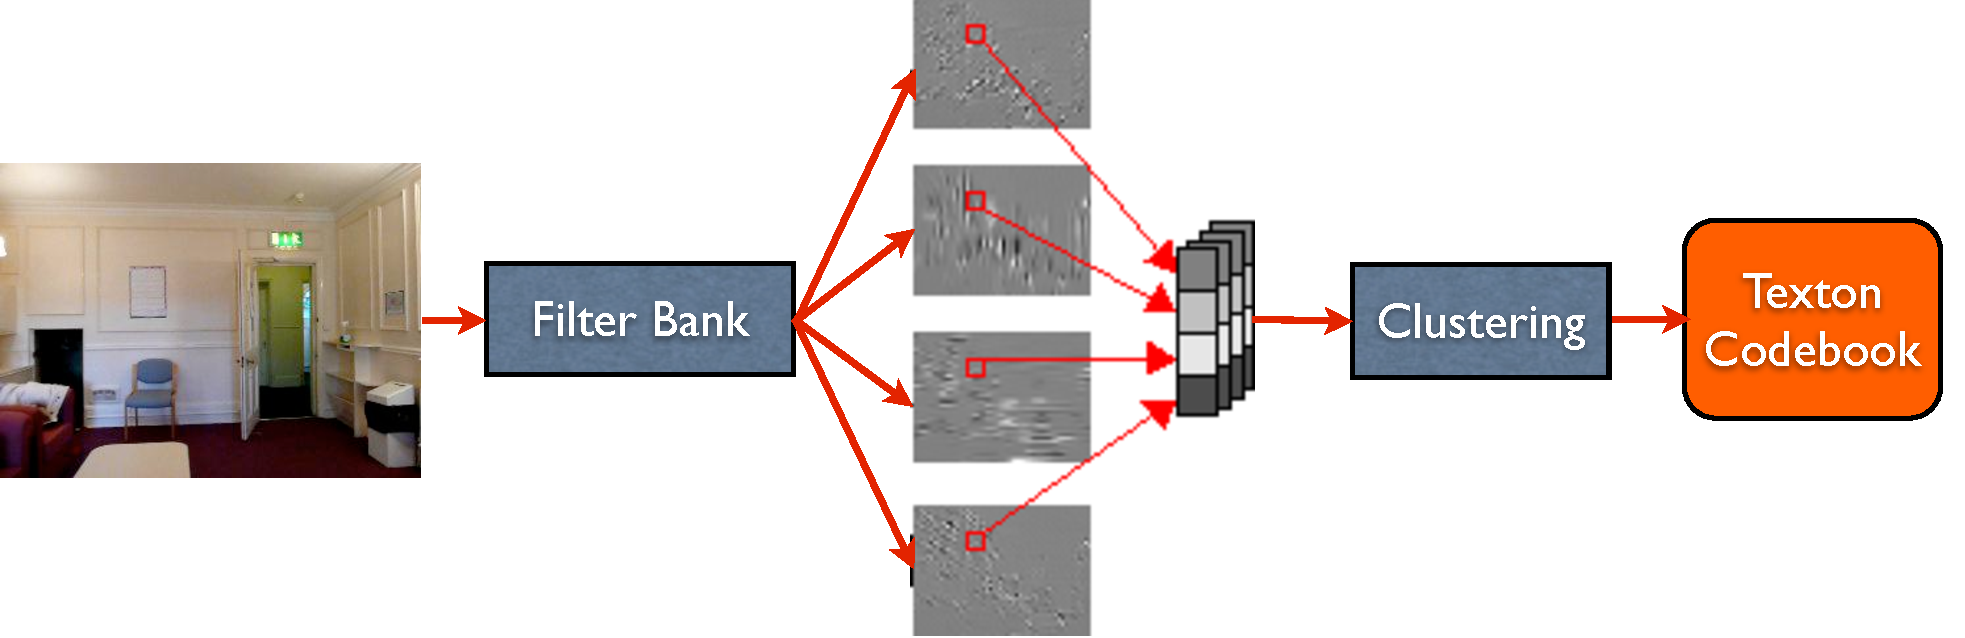
\includegraphics[width=\textwidth]{texton_process}
  \caption{The texton generation process.}
  \label{fig:texton-process}
\end{figure}

In the past textons have been successfully used to classify close--up
photos of materials such as wood, paper, and glass. Varma and
Zisserman \cite{Varma05} tackled this problem using the texton model
discussed above. After forming the texton map they proceed by counting
the occurrences of each texton, with the resultant histogram over
texton frequencies forming the model by which input images are matched
to their category. In their work, Varma and Zisserman apply a nearest
neighbour approach to classify the models, using the $\chi^2$
statistic to measure distances. Representing data by a histogram over
quantised features in this way has since become known by the
terminology ``bag--of--features'' or ``bag--of--words''.

\section{Textons for Scene Understanding}
Textons are a widely used and well--understood within the computer
vision community \cite{Zhu02,Varma05,Malik99}. However, their use has
mostly been limited to low--level image analysis tasks, such as
texture classification. We propose to use textons as the basis for
high--level reasoning tasks including scene classification. In the
remainder of this chapter we will develop a novel model by which to
utilise textons during inference. We begin in this section by
motivating the use of textons for this application.

Many place recognition systems rely upon an interest point detector
and descriptor to summarise input images
\cite{Fei-fei05,Cummins08}. This has proven effective for outdoor
environments as well as indoor environments that contain reasonably
distinctive landmarks. However, these systems are fundamentally
limited to a feature--centric view of the world in which only local
information about interest points is utilised.

We believe that there is un--leveraged information in the texture
structure within images, and that this can be used for scene
understanding tasks such as place recognition. Many images of indoor
scenes contain extremely poor visual information, particularly small,
empty environments like corridors and
foyers. \figref{low-saliency-frames} shows some examples of these. Yet
despite this information poverty, humans are capable of deducing much
from these images. For example, consider the image at the right of
\figref{low-saliency-frames}: there is barely one location here that
would yield a useful SIFT feature, yet a human can identify the part
of the environment that the image represents (a corner between wall
and ceiling), and a human familiar with the environment can easily
identify the room in which the image was captured. We think it is
clear that, in this case, humans are using a holistic understanding of
the image in which the edge structure together with the texture of the
surfaces is used to understand the image. We propose to use textons to
leverage this valuable information.

\begin{figure}[htp]
\centering
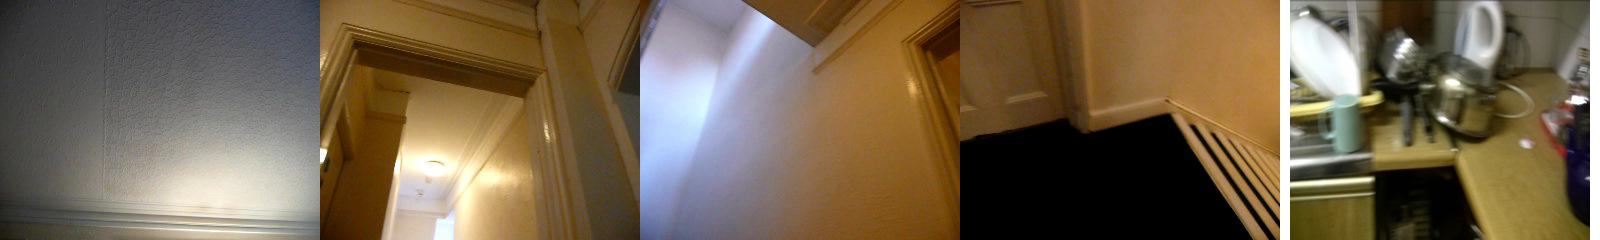
\includegraphics[width=\textwidth]{low_saliency.png}
\caption{Frames with low visual salience.}
\label{fig:low-saliency-frames}
\end{figure}

To investigate whether textons provide useful information about scene
structure, we collected video sequences of an indoor environment and
examined the textons generated by the algorithm described above. Our
dataset consisted of $10,555$ frames from $5$ rooms in a hostel. Some
qualitative findings are described in the following sections.

\subsection{Textons Select Salient Image Elements}
\figref{textons-generated} shows $25$ textons generated for this
dataset, in order of their frequency of occurrence. The first $7$
correspond to untextured regions of the image --- \ie
patches with near--uniform intensity. This is expected since the
majority of pixels lie within object or region boundaries, where
either the texture is too fine for the camera to detect (a carpet,
for example) or there simply is no texture (a white wall, for
example).

The next most frequent textons are those corresponding to edges and
bars at various orientations. Many image understanding algorithms
explicitly employ a line detector \cite{Forsyth02}, whereas in this
case the use of textons has allowed the system to learn to identify
these elements unsupervised.

At the other end of the frequency distribution, the least numerous
textons are those corresponding to image structures such as
junctions and line endpoints. These structures are also sought
explicitly in many image understanding algorithms \cite{Forsyth02},
whereas the use of textons selects these structures automatically and
unsupervised.

\begin{figure}[htp]
  \centering
  
\includegraphics[width=\textwidth]{texton_exemplars}
  \caption{\changedsinceviva{
      Textons identified for our dataset during the offline
      training stage. Each panel shows a representative image patch for
      one of the cluster identified by K--means. The patches were
      selected by identifying the feature closest to each cluster
      centre, and then extracting a small patch about the image position
      from which it arose. The textons are sorted by
      decreasing frequency from top to bottom, left to right. Image
      patches are converted to grayscale before filtering, but here we
      show them in colour to assist visualisation. The patches vary in
      size due to clipping near image boundaries (this does not affect
      clustering).
    }
  }
  \label{fig:textons-generated}
\end{figure}

\subsection{Textons Focus Attention on Salient Image Regions}
\figref{texton-freq-distr} shows the frequency of each texton within
our entire dataset. The most frequent textons at the left of the graph
account for a disproportionately large number of pixels, whereas the
textons towards the right account for a tiny minority. We have just
seen that it is precisely these minority textons that correspond to
the image elements that are most useful in image understanding, so in
this sense the use of textons has automatically focused attention on
the small fraction of pixels representing the most salient image
structures.

\begin{figure}[htp]
  \centering
  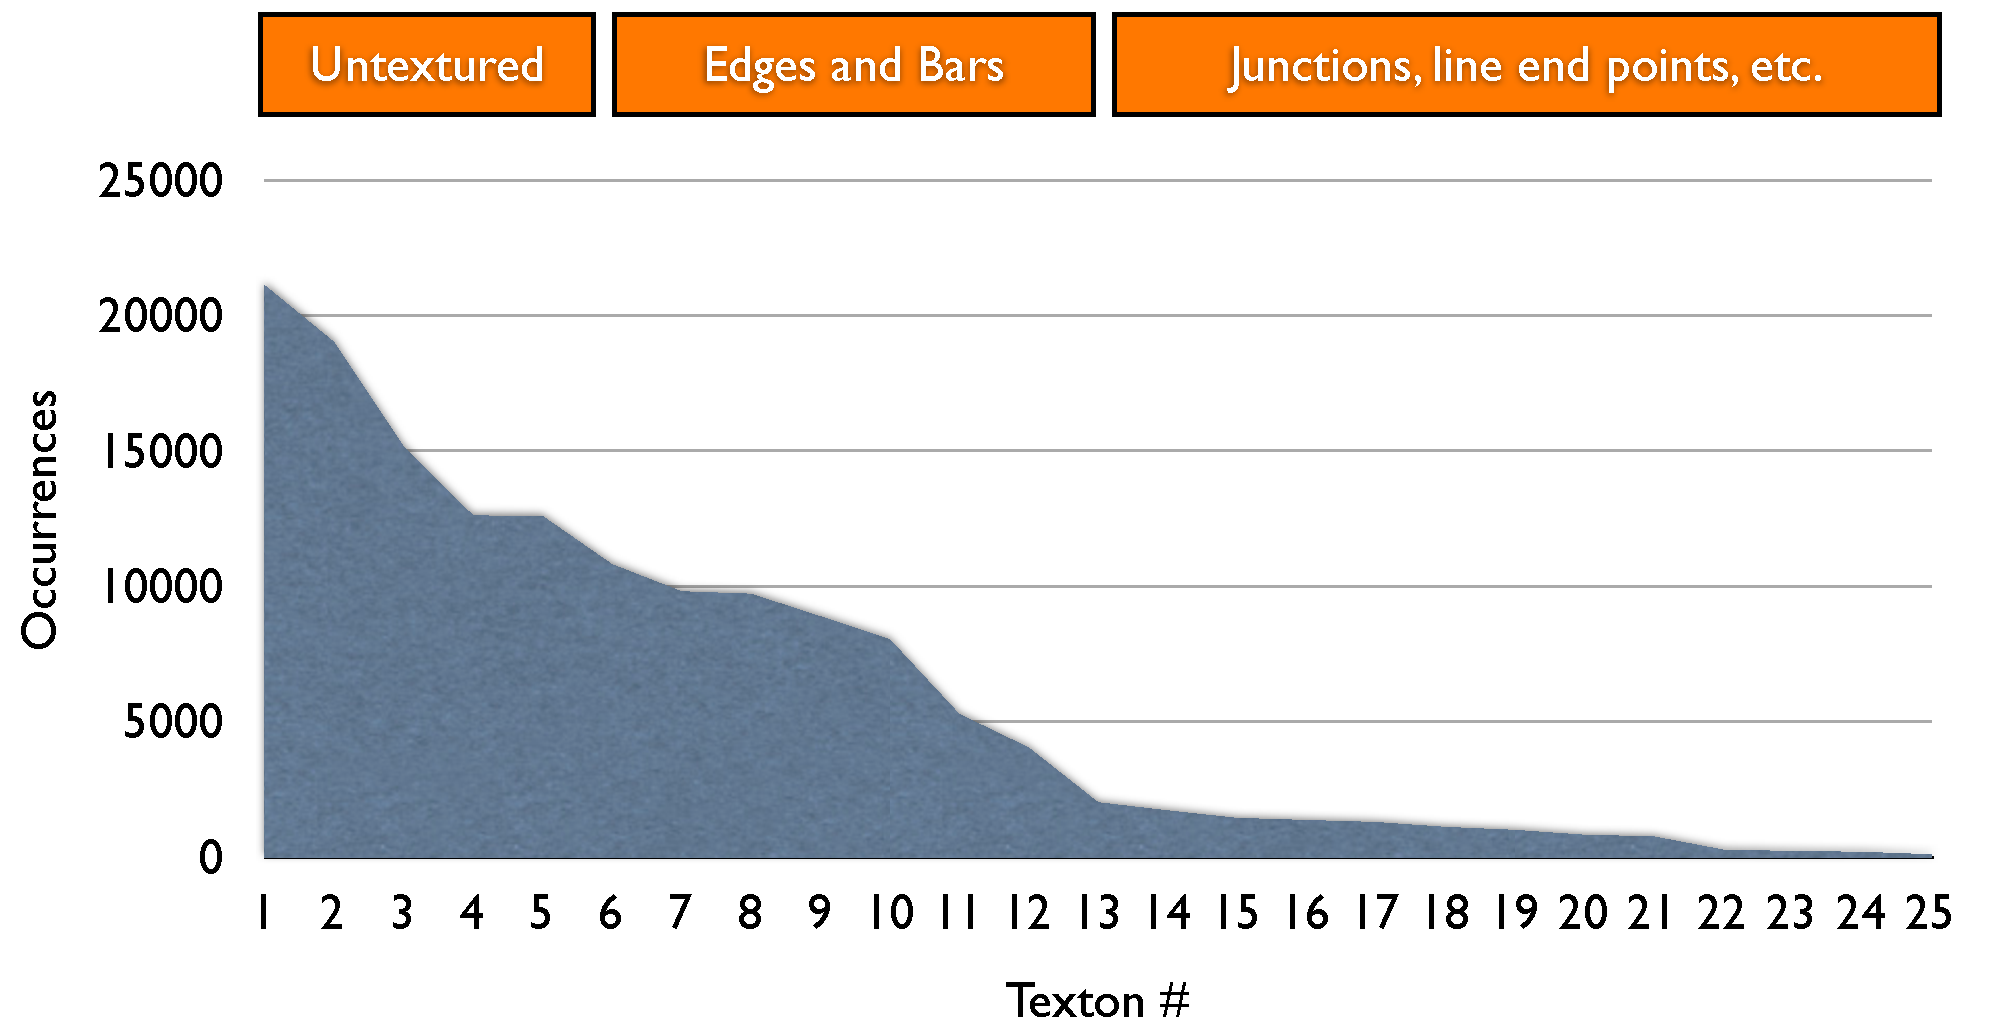
\includegraphics[width=0.8\textwidth]{texton_frequencies}
  \caption{Frequency distribution of textons. The texton generation
    process assigns more textons to describing salient but rare image
    structures such as junctions and line end points than it assigns to
    frequent but non--discriminative image regions such as textureless
    patches.}
  \label{fig:texton-freq-distr}
\end{figure}

\subsection{Textons Correlate With Scene Structure}
To further explore the relationship between textons and scene
structure we divided all frames within our dataset into three
orientation categories: ``straight'' (for which the camera's optical
axis was within $\pm 22.5\degrees$ of the horizontal), ``up'' (above
$22.5\degrees$), and ``down'' (below $22.5\degrees$). Next we computed
an average occupancy map for each texton within across each
category. Several per--texton heat--maps are shown in
\figref{eg-textons}. The first two rows show heat--maps for textons that
correspond roughly to ``floor'' and ``wall/ceiling''. We can see that
these reflect the image regions in which we would expect to find these
scene parts given the various camera orientations.

Perhaps the most instructive example of the texton/scene structure
relationship, however, is that of the textons that represent edge
elements, two of which are shown in the lower two rows of
\figref{eg-textons}. Consider the third row in this figure: The
stratification evident in the heat--map for downward--facing frames
indicates a common intersection somewhere above the image, whereas
that for the upward--facing frames indicates an intersection below the
image, and in the forward--facing frames the lines are close to
parallel. This, of course, is exactly what we would expect from our
understanding of projective camera geometry, but here our system has
automatically and without supervision captured these geometric
constraints (or at least some statistical form of them).

These illustration are simply indications that textons might provide
salient information of value for scene understanding. We describe our
model that explicitly relates these to each other in the next section.

\begin{figure*}[htp]
\centering
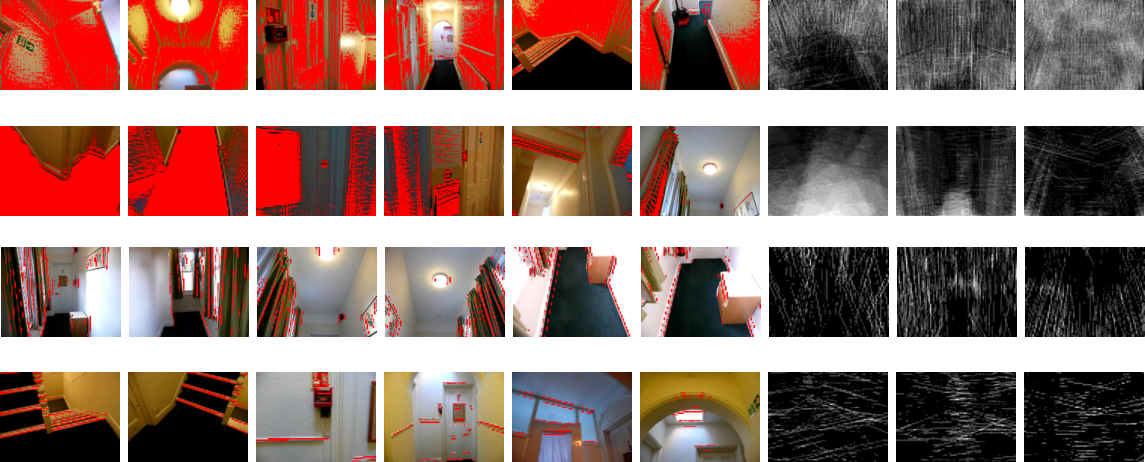
\includegraphics[width=\textwidth]{eg_textons.png}
\caption{Four example textons generated unsupervised for the camera
  orientation classification problem. From top to bottom the textons
  represent roughly ``wall or ceiling'', ``floor'', ``vertical edge'',
  and ``horizontal edge''. The six columns on the left show examples
  of where the texton was found. The three columns on the right show
  the average occupancy map over our dataset for images taken from an
  upwards--facing, horizontal, and downwards--facing camera (from left
  to right in the figure). The layout of the textons correlate
  strongly with camera orientation, which illustrates how our system
  is able to distinguish between camera orientations based on texton
  layout.}
\label{fig:eg-textons}
\end{figure*}

\section{Learning and Inference}
\label{sec:approach}
Having motivated the use of textons for image understanding we now
describe our probabilistic model that relates textons to scene
categories. For an input image $I$, we wish to discover the associated
place category $c$. For each category we are given a set of example
images at training time. We wish to model categories $c$ according
to the pixel locations in which textons appear within images
associated with each category. One popular approach is the
bag--of--features model \cite{Jebara03} but this would remove all
information about the locations of the textons, which as we have seen
is a principal source of salient information. Instead we propose a new
bag--of--texton--pairs model in which an image is represented as a
collection of observed texton pairs $\{(t_i, t_j, s_{i,j})\}$ where
$t_i$ and $t_j$ are texton labels and $s_{i,j}$ is the displacement
between the image locations at which they were observed. By
considering only displacements and not absolute pixel locations in our
model we gain some robustness to camera orientation.

For an image $I$ containing $N$ pixels there are $N^2$ such
pairwise observations. Our class--conditional likelihood is
\begin{equation}
P(I ~|~ c) = \prod_{i=0}^N \prod_{j=0}^N
P(t_i, ~ t_j, ~ s_{i,j} ~|~ c) \label{lik}
\end{equation}
where we have assumed independence between observations for
tractability. We compute the likelihood \eqref{lik} by estimating the
joint distribution $P(t_i,t_j,s_{i,j},c)$ using a histogram. We could
have used Parzen windowing \cite{Parzen62} for the continuous variable
$s_{i,j}$ but due to the very large number of samples we obtain for
each image, we found this to be unnecessary.

\changedsinceviva{
For images of reasonable size the cost of enumerating all $N^2$ texton
pairs is prohibitively expensive. We overcome this by overlaying an $M
\times M$ grid on the image and counting the occurrences of each
texton within each grid cell. We then enumerate all pairs of grid
cells and evaluate the texton pairs in aggregate. Hence for grid cells
$C_a$ and $C_b$ containing $n^a_i$ and $n^b_j$ instances of texton
$t_i$ and $t_j$ respectively, we evaluate $n^a_i n^b_j$ instances of
the observation $(t_i,t_j,s_{a,b})$ where $s_{a,b}$ is the distance
between the centres of the grid cells. We have lost some precision in
the texton locations since each texton is effectively moved to the
centre of the grid cell containing it, but our experiments show that
we are still able to capture sufficient salient information. We also
note that quantizing displacements in this way implicitly shares
information between similar displacements. One could think of this
operation as an efficient approximation to building the full joint
distribution and then smoothing along the displacement
axis.
}

During training we evaluate these aggregated observations by
multiplying the entry we make in the histogram by $n^a_i n^b_j$, and
during evaluation the aggregate observations correspond to
multiplications in the class--conditional log likelihood
\begin{eqnarray}
\log P(I ~|~ c) & = & \sum_{a=0}^{M^2} \sum_{b=0}^{M^2} \sum_{i=0}^K  \sum_{j=0}^K
 n^a_in^b_j \log P(t_i, ~ t_j, ~ s_{a,b} ~|~ c)
\end{eqnarray}
In both cases the aggregated observations can be evaluated in a single
step so the complexity is reduced from $O(N^2)$ to $O(M^4 K^2)$. In
practice we found that setting $M$$=$$8$, $K$$=$$25$ was sufficient to capture
much of the salient image information, while allowing our system to run
at video frame rate.

\section{Place Recognition}
\label{sec:place-recognition}
We applied our system to the problem of place recognition. Our data
set consisted of several video sequences captured in a hostel
using a low--quality camera with a resolution of $320 \times 240$,
which moved rapidly with the user's upper body. The sequences involved
frequent motion blur and rapid variations in camera orientation.

We labelled each frame with the place that it was captured in. There
were five labels: bedroom, kitchen, common room, garden, and
corridor. We gave all frames captured in corridors the same
label. This experiment does not correspond to place {\em category}
recognition since most of the labels included frames from only one
place instance. However, it is harder than strict landmark--style
localisation because, as shown in \figref{nonoverlapping}, many images
with the same label contain non--overlapping views of the room they
were captured in, yet the system is expected to recognise all of them
as belonging to the same place.

\begin{figure}[htp]
  \centering
  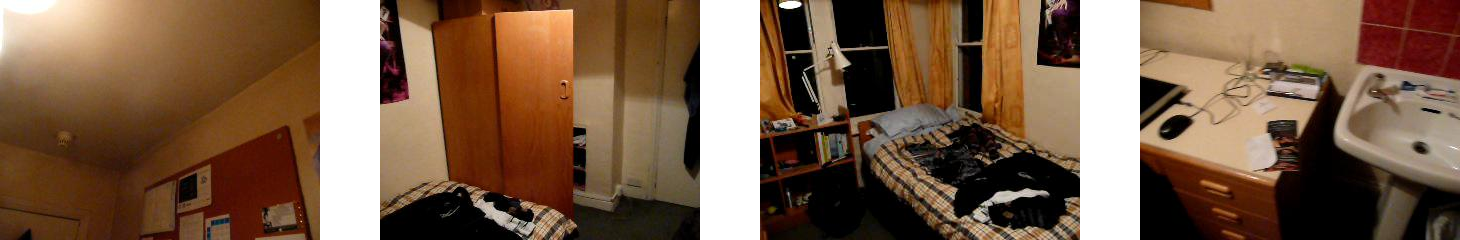
\includegraphics[width=\textwidth]{nonoverlapping.png}
  \caption{Four frames with the ``bedroom'' label. There are almost no
    overlapping scene parts but the system is required to (and did
    successfully) recognise each of them as part of the same place.}
  \label{fig:nonoverlapping}
\end{figure}

We compared our system with the gist descriptor of Torralba \etal and
a K--nearest--neighbours baseline, using vectorised grayscale images
as feature vectors for the latter. For the gist descriptor we used the
same Gabor filter bank that we used in our own system and we estimated
the class--conditional likelihood in feature space by building
Gaussian mixture models with the Gaussians constrained to be
spherical, exactly as described in \cite{Torralba03}.

Initially we used 230 frames for training and 490 frames for
evaluation (our training and evaluation sets were taken from separate
sequences). The results from this experiment are shown in the middle
row of \tableref{place-cla-results} and in
\figref{place-confusion}. Our system outperformed Torralba's by a
large margin. We suspected that the poor performance of Torralba's
system was due to the training data not sufficiently populating the
32--dimensional feature space. This exemplifies one of the major
advantages of our approach: the ability to learn from limited training
data. However, to show that this is not the \textit{only} advantage of
our approach we ran auxiliary experiments with larger and smaller
training sets. When the training set was enlarged our system
outperformed Torralba's by a significant but smaller margin, and when
the training set was decreased, the performance of our system
decreased only slightly whereas Torralba's system was unable to
estimate the Gaussian mixture due to the sparsity of training
samples. The latter case corresponds to just 20 examples per
label. These results are shown in the top and bottom rows of
\tableref{place-cla-results}.

Figures \ref{fig:pos-examples} and \ref{fig:neg-examples} show
positive and negative results from our system. Note how our system
recognises images containing disjoint views of a room as belonging to
the same place.

\begin{table}[htb]
  \centering
  \begin{tabular}{@{}p{40mm}p{30mm}p{30mm}p{40mm}@{}}
    \toprule
      No. training frames &
      This chapter &
      Torralba \etal &
      Nearest neighbours \\
    \midrule
      103 & \textbf{81\%} & --- & 45\% \\
      230 & \textbf{83\%} & 62\% & 52\% \\
      565 & \textbf{85\%} & 70\% & 55\% \\
    \bottomrule
  \end{tabular}
  \caption{Recognition rate for the place recognition problem with
    varying numbers of training examples. The reported accuracy is the
    mean over the on--diagonal elements of the confusion matrix. The
    left column reports the total number of training examples for all
    categories. For the experiment with 103 training examples we were
    unable to estimate the Gaussian mixtures required for the system
    of Torralba \etal due to the sparsity of the training
    examples. The nearest neighbours baseline was computed by resizing
    images to 64 by 64 pixels and comparing raw pixel intensities in
    the L2 sense.}
  \label{table:place-cla-results}
\end{table}

\begin{figure}[htp]
  \centering
  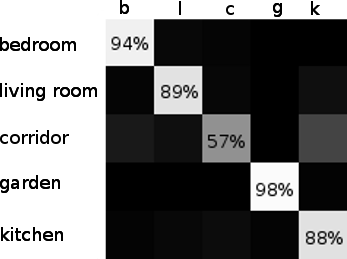
\includegraphics[width=0.4\textwidth]{place_confusion}
  \caption{Confusion matrix for place recognition. This figure
    corresponds to the bottom row of \tableref{place-cla-results}.}
  \label{fig:place-confusion}
\end{figure}

\begin{figure*}[htp]
\centering
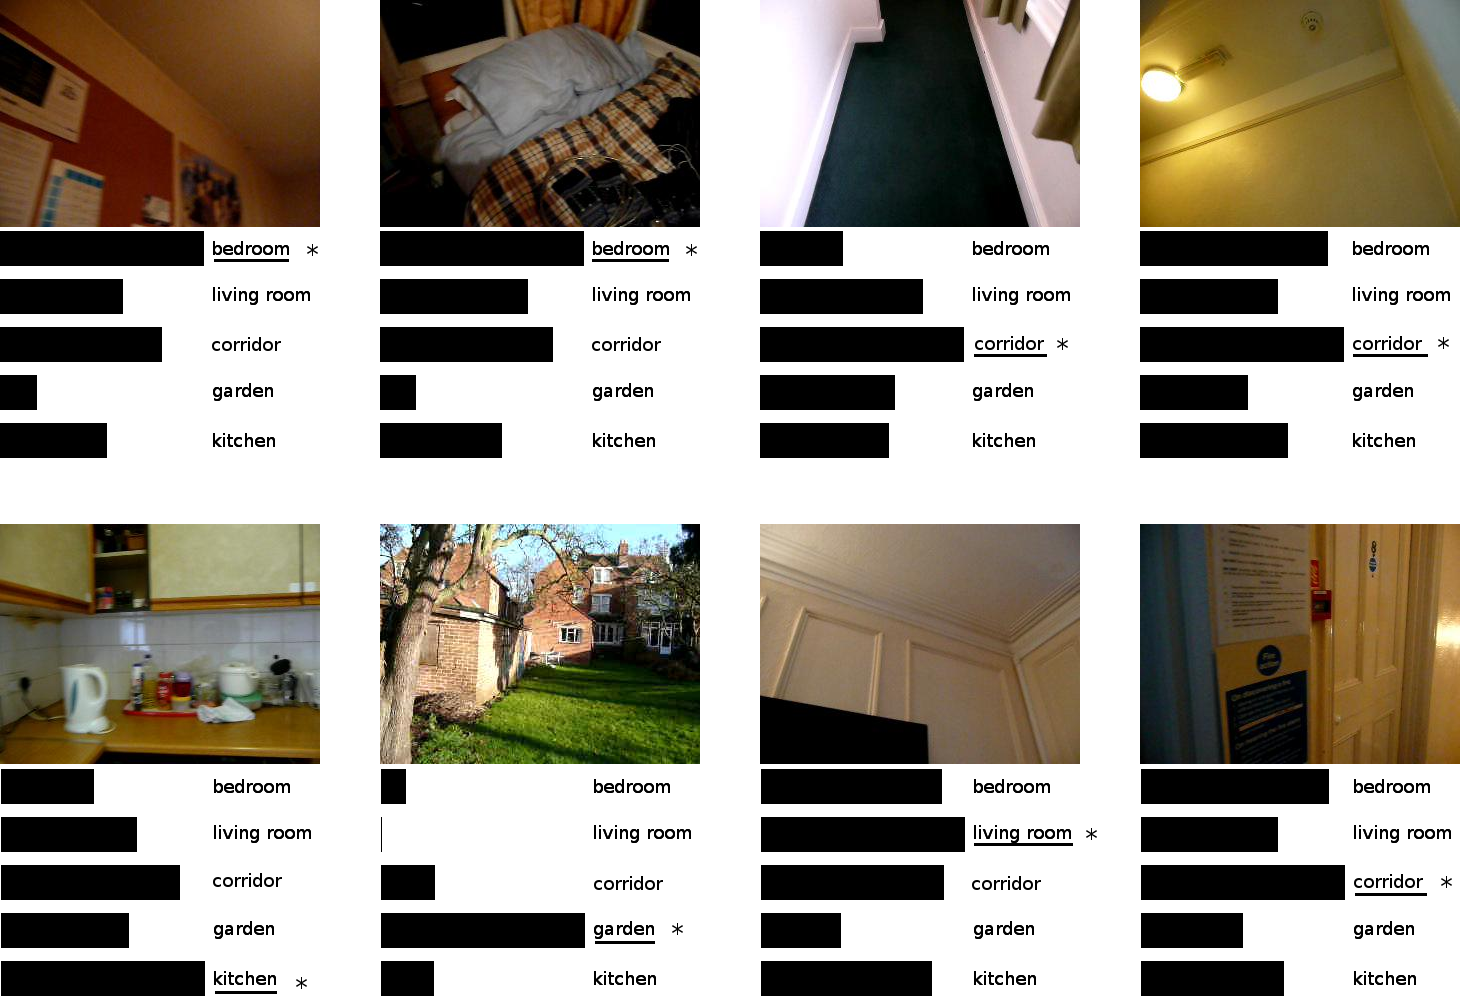
\includegraphics[width=\textwidth]{pos_examples.png}
\caption{Example frames for which our classifier produced the correct
  output. The ground truth label is underlined and the output from our
  system is starred. We show the posterior distribution over class
  labels in black. Note the variation between images with the same
  label, and the low quality of many images.}
\label{fig:pos-examples}
\end{figure*}

\begin{figure*}[htp]
\centering
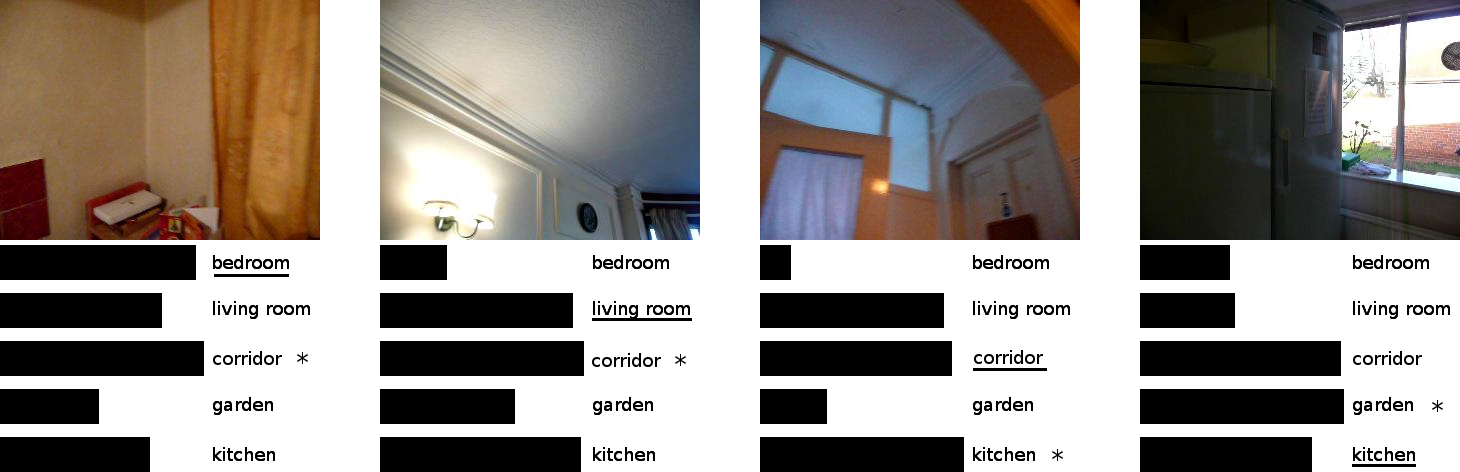
\includegraphics[width=\textwidth]{neg_examples.png}
\caption{Example frames for which our classifier failed. See caption
  of \figref{pos-examples}.}
\label{fig:neg-examples}
\end{figure*}

\section{Camera Orientation Classification}
\label{sec:camera-orientation}
In this section we show how our system can deduce a coarse camera
orientation from a single image. We are interested only in the tilt of
the camera with respect to the ground plane. Our intention is to make
a rapid but coarse estimate of camera orientation. We pose the problem
as a classification task with three labels: ``up'', ``straight'', and
``down''. The ``straight'' label represents images taken with the
camera axis parallel to the ground plane, plus or minus
$22.5^{\circ}$, and the ``up'' and ``down'' labels represent all
orientations facing further upwards or downwards respectively (see
\figref{camorients}).

\begin{figure}[htp]
  \centering
  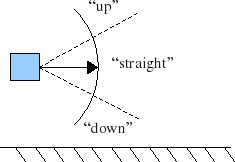
\includegraphics[width=0.4\textwidth]{camorients}
  \caption{Definition of the labels for camera orientation recognition.}
  \label{fig:camorients}
\end{figure}

We captured three sequences in which the camera orientation was fixed
within one of the above orientation ranges. We included footage from
five different places (the same rooms used in the previous section) but
we labelled the frames according to orientation only. This represents
a difficult classification task because the system must learn
properties that correlate with camera orientation but are not tied to
the appearance of a particular room. We then trained our system to
distinguish between the three orientation categories as in the
previous section.

We again compared with the ``gist'' of Torralba {\em et al.} and a KNN
baseline. We ran auxiliary experiments with an enlarged training set
as in the previous section. The results of these experiments are shown
in \tableref{orient-cla-results} and \figref{orient-confusion}. Our
system again outperformed both other classifiers by a significant
margin. Some example frames for which our system correctly identified
the camera orientation are shown in \figref{eg-orients}. Of particular
interest is our system's ability to generalise across images taken
with the same camera orientation at several different locations.

\begin{table}[htb]
  \centering
  \begin{tabular}{@{}p{40mm}p{30mm}p{30mm}p{40mm}@{}}
    \toprule
      No. training frames &
      This chapter &
      Torralba \etal &
      Nearest neighbours \\
    \midrule
      88 & \textbf{70\%} & 61\% & 59\% \\
      728 & \textbf{79\%} & 63\% & 59\% \\
    \bottomrule
  \end{tabular}
    \caption{Camera orientation classification results using small and
      large training sets. The reported accuracies are the average of
      the on--diagonal entries in the confusion matrix. In this case
      we were able to estimate the Gaussians for Torralba's system
      using only 88 training examples because there were fewer categories
      than in the place recognition problem. The nearest neighbours
      baseline was computed by resizing images to 64 by 64
      pixels and comparing raw pixel intensities in the L2 sense.}
  \label{table:orient-cla-results}
\end{table}

\begin{figure}[htp]
  \centering
  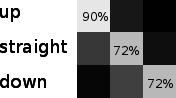
\includegraphics[width=0.25\textwidth]{orient_confusion}
  \caption{Confusion matrix for camera orientation
    classification. This figure shows results corresponding to the
    bottom row in \tableref{orient-cla-results}.}
  \label{fig:orient-confusion}
\end{figure}

\begin{figure}[htp]
\centering
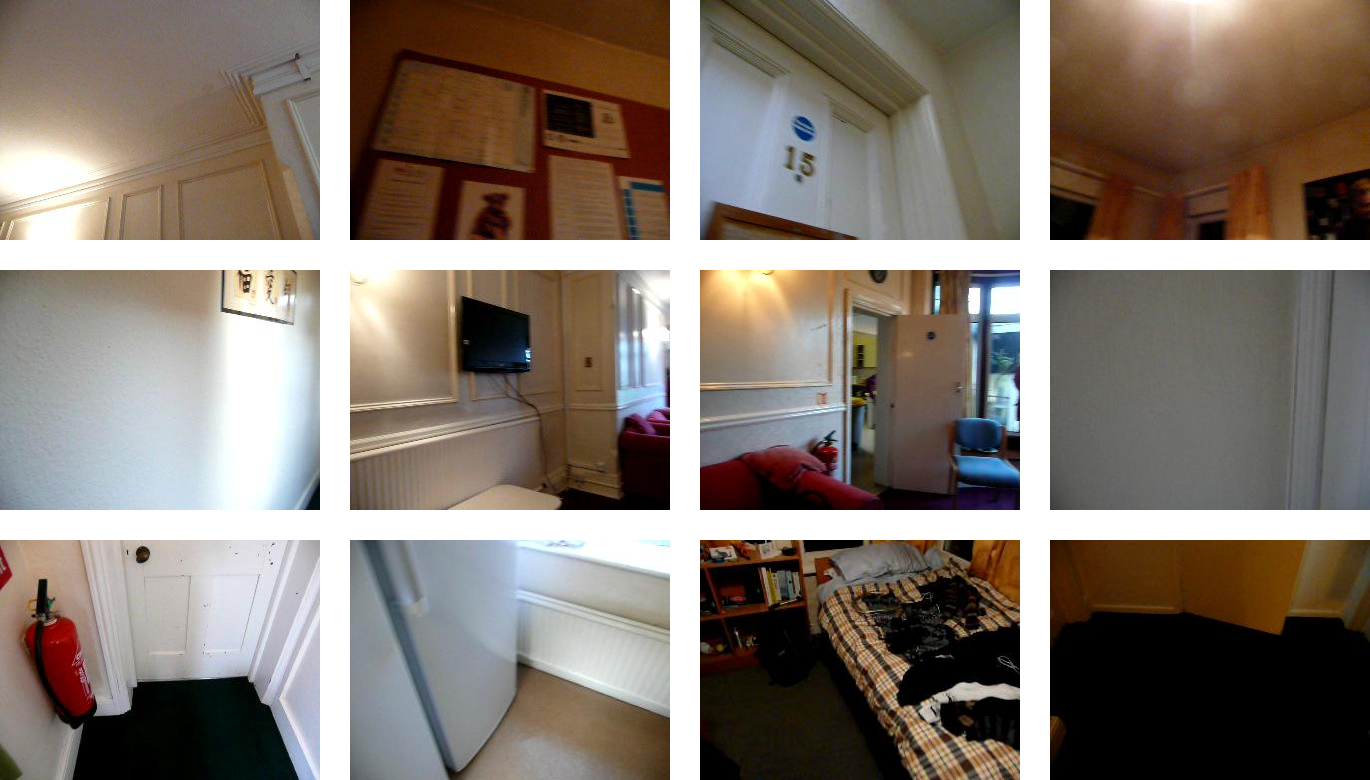
\includegraphics[width=\textwidth]{orient_egs.png}
\caption{Twelve frames for which our system correctly identified the
  camera orientation. From the top to bottom the rows contain images
  from the ``up'', ``straight'', and ``down'' classes.}
\label{fig:eg-orients}
\end{figure}


\section{Computational Concerns}
The most computationally demanding aspect of our system is the
convolutions needed to generate the pixel features. In this section we
describe several optimisations for the convolution operation. Timing
results are shown in \tableref{convolve-timing} at the end of this
section.

\subsection{Separable Kernels}
The Gabor function, which we use to generate pixel features, in its
canonical form is a complex--valued function and can be trivially
separated. However, in our work we use just the real part,
\begin{eqnarray}
  H_{real}(x,y) & = & g_2(x,y) \cos(kx\cos\theta + ky\sin\theta) ~,
\end{eqnarray}
where $g_2$ is the two--dimensional Gaussian
function. This can be written as the difference between two separable
function as
\begin{eqnarray}
  %H_{real}(x,y) & = & g_2(x,y) \cos(ax + by)\\
  %  & = & g_1(x)g_1(y) \Bigl(\cos ax\cos (by) - \sin ax \sin by
  %    \Bigr) \label{sep2}\\
   H_{real}(x,y) & = & \Bigl(g_1(x)\cos ax\Bigr) \Bigl(g_1(y)\cos by\Bigr)
      - \Bigl(g_1(x)\sin ax\Bigr)\Bigl(g_1(y)\sin by\Bigr)
\end{eqnarray}
where $g_1$ is the one--dimensional Gaussian function and we have used
the cosine expansion formula. We implement this by running two
separated convolutions and then taking their difference, which is
significantly faster than performing the original convolution.

\subsection{Parallelization over filters}
Generating the pixel features requires convolving an input image with
12 different filters. To leverage the parallelism of
modern multi--core CPUs we execute the convolutions in parallel where
possible. This approach allows parallelization within a single scale,
but requires synchronisation upon completion of each scale due to the
down--sampling operation.

\subsection{Parallelization over pixels}
Modern graphics hardware allows efficient parallelization of
small--scale computations such as per--pixel operations. This is is
well suited to performing convolutions since each output pixel is
functionally independent of all others. To leverage this we
implemented convolutions using a C--like language designed
specifically for programming graphics hardware. We note that further
improvements may be possible since under the current implementation,
much time is spent transferring data between the CPU and GPU, in
comparison to which the time spent performing the convolutions is
small. This bottleneck could be partially avoided if we performed the
texton labelling in the GPU and transferred only the final texton map
back to the CPU.

\subsection{Timing results}
Results from timing evaluations are shown in
\tableref{convolve-timing}. The GPU strategy outperforms all
others. It improves over the baseline strategy by a factor of $5$ for
the $320 \times 240$ image and by a factor of $6$ for the $640 \times
480$ image.


It is interesting to note \changedsinceviva{that when} the image is
enlarged to include four times as many pixels, the three CPU--based
strategies degrade by a factor very close to four, whereas the GPU
implementation degrades by a factor closer to three. This indicates
that this task saturates CPU performance but that a significant
overhead remains in the GPU implementation. This matches our
observation in the previous section that transmitting data between the
CPU and GPU consumes much time, and that further performance
improvements are possible.



\begin{table}[htp]
  \centering
  \begin{tabular}{@{}p{40mm}p{20mm}p{20mm}p{20mm}p{20mm}@{}}
    \toprule
      & \multicolumn{2}{c}{\textbf{320 $\times$ 240}}
      & \multicolumn{2}{c}{\textbf{640 $\times$ 480}} \\
      \textbf{Strategy} &
      \textbf{Per Frame} &
      \textbf{Frame Rate} &
      \textbf{Per Frame} &
      \textbf{Frame Rate} \\
    \midrule
      No parallelization & 115.0ms & 8.69Hz & 463.6ms & 2.16Hz \\
      Filter--parallel & 38.0ms & 26.3Hz & 148.0ms & 6.76Hz \\
      Image--parallel & 32.1ms & 31.2Hz & 125.6ms & 8.02Hz \\
      Pixel--parallel (GPU) & 23.5ms & 42.5Hz & 78.1ms & 12.80Hz \\
    \bottomrule
  \end{tabular}
  \caption{Timing results for the four parallelization strategies. Each
    strategy was evaluated for two image sizes. All strategies utilise
    separated filters. Results are averages over 10 invocations.}
  \label{table:convolve-timing}
\end{table}

\section{Conclusions}
In this chapter we have shown that texture structure can be leveraged
to deduce high--level information about image scenes. We have
motivated the use of textons for this purpose with several qualitative
examples, and have presented results from two in--depth
experiments. In both cases our system based on relative displacements
between textons obtains highly encouraging results. Furthermore, by
utilising graphics hardware our system is capable of operating at
video frame rate.

%% We also note an intruiging line of investigation in which we could
%% treat the labelling process as a classification task with the values
%% from a neighbourhood about a pixel as inputs and the texton labels as
%% output. Since the filters only use local information anyway, it seems
%% possible to build an accurate classifier to operate on raw pixel
%% values, which would avoid both the convolution and nearest--neighbour
%% matching steps. The challenge, of course, would be to build a
%% classifier fast enough that this substitution resulted in a beneficial
%% trade--off. Perhaps randomized forrests would be suitable here. We
%% intend to pursue this line of investigation only if it is necessary
%% to achieve real--time performance.

%% \section{Choice of Filter Banks}

%% The use of filter banks in computer vision long pre--dates the texton
%% literature. A wide variety of kernel functions have been proposed such
%% as difference-- and derivative--of--Gaussians (¬cite), wavelets (Gabor
%% filter are particularly popular ¬cite), steerable pyramids
%% \cite{Freeman91}, and many others. Motivations for choosing one kernel
%% over another include expressiveness, orthogonality, efficiency,
%% simplicity, invariance to image transformations such as rotations
%% (¬cite), and the ability to reconstruct the original image from its
%% filtered form.

%% Our experience indicates that, among those kernel functions in
%% widespread use today, our system is largely unaffected by the specific
%% kernel chosen. That is not to say that the choice of kernel function
%% is unimportant \textit{per se}, but rather that, for our purposes, many
%% modern kernel functions provide equal amounts of salient information
%% from which our system is capable of learning. We chose the Gabor
%% kernel because of its theoretical basis in wavelet theory, its
%% simplicity of implementation, and its separability.

%% Varma and Zisserman \cite{Varma03} have suggested that filter banks
%% may not be necessary for texture classification at all. They
%% demonstrate that filter banks can be replaced by simply using the
%% values in a 9--neighbourhood about each pixel as that pixel's feature
%% vector, in which case their texture classifier performs equally as
%% well as when filter banks are used. We have not investigated whether
%% such a strategy would is suitable for our task. We intend to
%% experiment with this idea because from an efficiency point of view
%% avoiding the need for the convolution step entirely is attractive.


%%%%%%%%%%%%%%%%%%%%%%%%%%%%%%%%%%%%%%%%%%%%%%%%%%
%
\def\localpath{Geometry}
\graphicspath{{\localpath/figures/}}
\chapter{The Geometry of Indoor Environments}
\label{chap:geometry}
% If you like chapter abstracts ...
%\begin{quote}{\em This chapter describes an application of 

The abstract text is put into Ch\#/ab\#.tex, where
\# is the chapter number.
}\end{quote}
\begin{quote}
  This chapter develops the idea that comprehensive scene
  understanding at the level of objects, actions, and surfaces
  requires at least a rudimentary understanding of the high--level
  geometry of the environment. There are many ways to capture such
  coarse geometry; here we argue that the indoor Manhattan
  representation is an excellent choice in terms of the salient
  geometric information it captures, its simplicity, and the elegant
  inference procedures it permits. This chapter focuses on analysing
  the model itself, leaving algorithms and empirical results to later
  chapters. This constitutes the first comprehensive definition and
  analysis of indoor Manhattan environments in the literature (though
  not the first account \textit{per se} \cite{Lee09}). The primary
  contributions of this chapter are a derivation of the ``vertex'' and
  ``seam'' parametrisations, and the description of several properties
  of these parametrisations that will prove crucial to the development
  of the following chapters.\footnotemark
\end{quote}

\footnotetext{
{ \setlength{\parindent}{0pt} 
  This work was published in part in:\\
  \textit{Flint, Mei, Murray, and Reid,} ``A Dynamic Programming
  Approach To Reconstruction Building Interiors'', in \textit{Proceedings
    of the 2010 European Conference on Computer Vision}\quad\cite{Flint10eccv}
}
}

\begin{figure}[tb]%
  \centering
    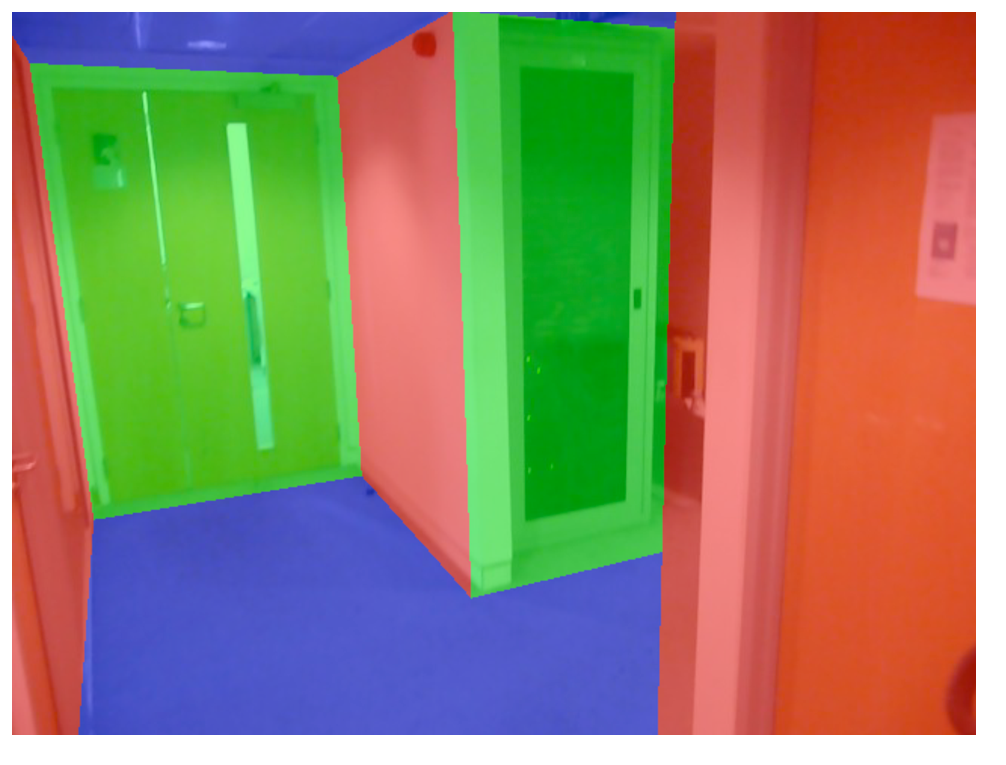
\includegraphics[width=0.45\textwidth]{manhattan-eg2}
    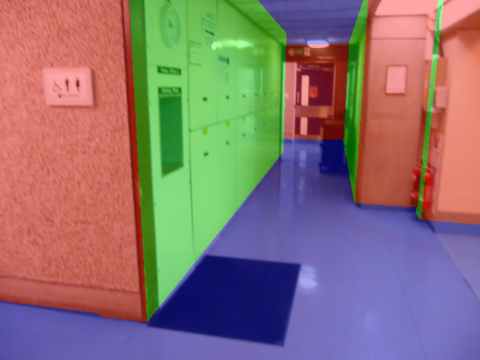
\includegraphics[width=0.45\textwidth]{manhattan-eg1.png}
    \caption{Two examples of indoor Manhattan environments.}
  \label{fig:geometry-egs}
\end{figure}

%%%%%%%%%%%%%%%%%%%%%%%%%%%%%%%%%%%%%%%%%%%%%%%%%%%%%%%%%%%%%%%%%%%%%%%%
\section{Introduction}

The preceding chapter described an approach to scene understanding in
which raw image features were connected directly to high--level
quantities such as scene categories. This chapter begins the
development of a more sophisticated model in which pixel--level
features are connected to high--level quantities via an unobserved
intermediate level representing scene geometry. We focus on recovering
this intermediate representation, leaving the application to specific
classification tasks to future work. There are a number of reasons to
see geometry as central to scene understanding. For an intuitive
demonstration, consider the information conveyed by the red, green,
and blue regions in \figref{geometry-egs}. These regions have very low
fidelity (the entire model is defined by just a handful of polygons),
yet it is clear that they convey considerable information about the
likely locations of various objects, the scale at which those objects
would appear, and how they would interact.

There are many choices for the representation of the
intermediate--level variables; the following desiderata summarise the
requirements relevant to our goals.
\begin{enumerate}
  \item{\textbf{Salience.} Of all the information present at the
    image level, the intermediate variables should capture as much of
    the information that is \textit{relevant} to inferring the
    high--level quantities of interest as possible.}
  \item{\textbf{Compression.} The intermediate representation should
    discard as much irrelevant information as possible. All else
    equal, we prefer succinct representations of the world for
    efficiency reasons. See MacKay \cite{MacKay2003} for a discussion
    of the connection between compression and learning.}
  \item{\textbf{Tractability.} All else equal, we prefer
    representations that lead to simple and efficient inference
    algorithms. A simple model for which inference is tractable
    may be preferable to a slightly more expressive model in which
    one must rely on approximate inference procedures with
    poorly--understood convergence properties.}
  \item{\textbf{Simplicity.} All else equal, we prefer representations
    consisting of quantities that are intuitive to humans.}
  \item{\textbf{Generality.} The chosen representation should be
    applicable to a wide variety of real--world environments.}
\end{enumerate}

We have chosen to work with the indoor Manhattan representation, in
which the world is built up from a floor plane, a ceiling plane, and a
sequence of vertical wall segments. This representation was originally
proposed by Lee \etal \cite{Lee09}. Indoor Manhattan environments are
a sub--class of general Manhattan environments, which simply specify
surfaces in three mutually orthogonal directions. Indoor Manhattan
scenes satisfy the desiderata above for the following reasons.
\begin{itemize}
  \item{\textbf{Compression and salience.} As described above, the
    geometric entities present in the indoor Manhattan representation
    correlate well the high--level quantities of interest for scene
    understanding. The models shown in \figref{geometry-egs} consume
    just a few hundred bytes, yet capture much of the information
    present in the original image data, which consumes three orders of
    magnitude more space. The point here is not to save disk space,
    but to demonstrate that indoor Manhattan models efficiently capture
    salient information.}
  \item{\textbf{Simplicity.} Indoor Manhattan models are composed of
    quantities that have 
    have natural semantics, being associated with entities such as the
    floor, walls, and ceiling of an environment.}
  \item{\textbf{Generality.} Indoor Manhattan models can represent
    many environments exactly or approximately; even those that do not
    conform exactly to the assumptions of the model. We expand on this later.}
  \item{\textbf{Tractability.} Indoor Manhattan scenes have special
    geometric structure that permits an elegant ``seam''
    representation. This in term leads to efficient and exact
    inference algorithms for a range of sensor models, and an
    attractive learning algorithm. This are the subject of the ensuing
    chapters.}
\end{itemize}

By adopting the indoor Manhattan representation we are \textit{not}
restricted to working with \textit{ideal} indoor Manhattan
environments --- environments free of clutter, occlusions, windows,
or other deviations from our assumptions. Rather, the point is to take
account of such deviations in the probabilistic model relating image
features to scene structure. For example, the model we present for
depth measurements in \chapref{inference} explicitly marginalises over
the possibility that a given depth measurement corresponds to a
clutter object, an object observed through a window, or an erroneous
measurement. Thus we cast the Manhattan scene geometry as a latent
variable to be inferred in the presence of noise, clutter, and
occlusions, rather than as a complete description of everything we
might observe. Empirical results in forthcoming chapters show many
examples of our system working in real--world environments that are
very far from ideal indoor Manhattan scenes, containing poor lighting
and noisy images in addition to clutter, windows, and
non--Manhattan--aligned surfaces.

However, this chapter focuses on analysing the representation itself,
and so is concerned with ideal indoor Manhattan scenes. The
contributions of this chapter are (1) the first comprehensive
definition of the indoor Manhattan assumption; (2) two novel
representations for indoor Manhattan scenes; and (3) a number of minor
results connecting these representations and providing other insights
crucial to the ensuing chapters. As mentioned above, this chapter does
not contain any experimental results, though it does provide the
conceptual infrastructure that the remainder of this thesis builds
on. We begin by defining indoor Manhattan scenes, then we discuss our
first representation in terms of floorplans, followed a description of
the ``vertex'' and ``seam'' parametrisations that will be used in
following chapters. \secref{misc-geometry} contains a number of minor
deductions of relevance to the ensuing chapters, then we close with a
brief conclusion.

%%%%%%%%%%%%%%%%%%%%%%%%%%%%%%%%%%%%%%%%%%%%%%%%%%%%%%%%%%%%%%%%%%%%%%%%
\section{Indoor Manhattan Environments}

Let a reconstruction $\Reconstruction$ consist of a set of polygons
$\Poly_i$ with vertices $\vertex_j\in\Rthree$. An \textit{indoor
  Manhattan reconstruction} is a reconstruction $\Reconstruction$ with
the following properties.
\begin{enumerate}
\item{\textit{Each polygon is oriented in one of three mutually
    orthogonal directions}. Formally, for each pair of polygons
  $\Poly_i,\Poly_j \in \Reconstruction$ with unit--length normals
  $\normal_i,\normal_j$,
  \begin{equation}
    \normal_i \cdot \normal_j \in \{0,1\}
  \end{equation}
}
\item{\textit{There is a floor plane and a ceiling plane}. Formally,
  there exists some direction $\vertnormal$ and a pair of real
  numbers $\zfloor, \zceil$ such that each polygon
  $P\in\Reconstruction$ with normal $\normal=\vertnormal$ has
  vertices $\vertex$ satisfying
  \begin{equation}
    \vertex \cdot \vertnormal \in \{\zfloor, \zceil\}
  \end{equation}
}
\item{\textit{Vertical walls extend from floor to ceiling}. Formally, if
  $\normal_i \neq \vertnormal$ then we say that $\Poly_i \in
  \Reconstruction$ is a \textit{vertical} polygon. This
  condition is satisfied if and only if each vertex $\vertex$ of
  each vertical polygon satisfies
  \begin{equation}
    \vertex \cdot \vertnormal \in \{\zfloor, \zceil\}
  \end{equation}
}
\item{\textit{The edges of walls are vertical}. Formally, if
  $\vertex\in\Poly$ and $\vertex\cdot\vertnormal=\zfloor$, then
  $\exists\othervertex\in\Poly$ such that
  \begin{equation}
    \othervertex \cdot \vertnormal = \zceil
  \end{equation}
  and
  \begin{equation}
    \othervertex = \vertex + \ScaleParam \vertnormal
  \end{equation}
  for some $\ScaleParam \in \Reals$.
}
\end{enumerate}

We assume a pinhole camera mapping homogeneous world coordinates
$\vect{X}\in\Rfour$ to homogeneous image coordinates $\vect{x}\in\Rthree$
according to
\begin{equation}
  \vect{x} = 
  \CamMatrix \begin{bmatrix} \CamR & \CamTr \end{bmatrix} \vect{X} ~,
\end{equation}
where $\CamMatrix$ is a $3 \times 3$ homography, $\CamR$ is a
3--dimensional rotation matrix, and $\CamTr$ is a 3--dimensional
translation.

We define an indoor Manhattan \textit{scene} as a reconstruction
together with a camera viewpoint, subject to the following additional
constraints.
\begin{enumerate}
  \item{The camera centre $\vect{c}$ is located between the floor
    and ceiling planes,
    \begin{equation}
      \zfloor < \vect{c} \cdot \vertnormal < \zceil
    \end{equation}
  }
  \item{The reconstruction is closed relative to the camera
    viewpoint. Formally, for each viewing direction $\vect{x}$ there
    is some polygon $\Poly\in\Reconstruction$ containing a point
    $\vect{X}$ that projects to $\vect{x}$.
  }
\end{enumerate}

In general we will assume that scenes consist only of those polygons
visible to the camera. Since reconstructions consists of a finite
number of polygons and our camera model is linear, it can be shown
that an indoor Manhattan reconstruction truncated to a view
frustum remains an indoor Manhattan reconstruction as defined
above.

%%%%%%%%%%%%%%%%%%%%%%%%%%%%%%%%%%%%%%%%%%%%%%%%%%%%%%%%%%%%%%%%%%%%%%%%
\section{Floorplans}

The polygonal representation for indoor Manhattan environments is
inconvenient for our purposes. A more useful representation is a
\textit{floorplan}, in which walls are represented as line segments
in the $XY$ plane. Formally, we define a floorplan $\Floorplan$ as a
tuple $(\SceneR,\Zs,\Polyline)$, where
\begin{itemize}
  \item{$\SceneR$ is a 3--dimensional rotation;}
  \item{$\Zs=(\zfloor,\zceil)$ is a pair of scalars defining the floor
    and ceiling planes,
    \begin{eqnarray}
      \Pfloor &=& \{ \vect{x} ~|~ \vect{x} \cdot [0~0~1] = \zfloor \}\\
      \Pceil  &=& \{ \vect{x} ~|~ \vect{x} \cdot [0~0~1] = \zceil \} ~;
    \end{eqnarray}
  }
  \item{$\Polyline=\{(\startpt_i,\enpt_i)\}_{i=0}^M$, is a set of line
    segments defining walls, $\startpt_i,\enpt_i \in \Rtwo$.}
\end{itemize}

A floorplan $\Floorplan$ is converted to a reconstruction as
follows. First, extrude each line segment vertically out of the floor
plane to meet the ceiling plane, resulting in a set of vertical
planes. Next, add polygons for the floor and ceiling planes, which may
simply be sufficiently large polygons parallel to the $XY$
plane. Finally, apply the coordinate transform $\SceneR$. Formally,
the reconstruction corresponding to a given floorplan is given by
$\Reconstruction = \{ ( \vect{p}_i, \vect{q}_i, \vect{r}_i, \vect{s}_i
) \}$ where
\begin{eqnarray}
  \vect{p}_i &=& \SceneR \begin{bmatrix} \startpt_i \\ \zfloor \end{bmatrix} \\
  \vect{q}_i &=& \SceneR \begin{bmatrix} \enpt_i \\ \zfloor \end{bmatrix} \\
  \vect{r}_i &=& \SceneR \begin{bmatrix} \enpt_i \\ \zceil \end{bmatrix} \\
  \vect{s}_i &=& \SceneR \begin{bmatrix} \startpt_i \\ \zceil \end{bmatrix}
\end{eqnarray}

For the remainder of this chapter we use the term ``corner'' to refer
to a point at which two line segments in the floorplan meet. In 3D, a
corner is therefore a vertical seam at which two walls meet. This
contrasts with the usual computer vision terminology in which a corner
corresponds to a point in 3D.

\subsection{Images of Floorplans}

\newcommand\worldpt{\vect{v}}
\newcommand\otherworldpt{\vect{u}}
\newcommand\imagept{\vect{p}}
\newcommand\otherimagept{\vect{q}}

The remainder of this thesis will be simplified considerably if we can
assume that vertical lines in the world appear vertical in image
coordinates. To that end we define the following homography:
\begin{equation}
  \label{eq:rectifier}
  \Rectifier =
  \begin{pmatrix}
    \vvpt \times \ez \\
    \vvpt \\
    \vvpt \times \ez \times \vvpt
  \end{pmatrix} ~.
\end{equation}
where $\vvpt$ is the vertical vanishing point and $\ez=[0~0~1]$.
Let $\Image'$ be the image formed by applying the homography $\Rectifier$ as a
coordinate transform to $\Image$,
\begin{equation}
  \label{eq:rectification}
  \Image'(\vect{x}) = \Image(\Rectifier \vect{x})
\end{equation}
where we are implicitly working in homogeneous coordinates. We say
that $\Image'$ is \textit{vertically rectified} in the sense that any
line containing $\vvpt$ in the original image will be mapped to a
vertical line in the output image. \changedsinceviva{To confirm this we note that
$\Rectifier$ maps $\vvpt$ to vertical infinity as the following
derivation shows.}
\begin{eqnarray}
  \Rectifier ~ \vvpt &=&   
    \begin{pmatrix}
      \vvpt \times \ez \\
      \vvpt \\
      \vvpt \times \ez \times \vvpt
    \end{pmatrix} \vvpt \\
  &=&
    \begin{pmatrix}
      0 \\ \vvpt \cdot \vvpt \\ 0
    \end{pmatrix} ~.
\end{eqnarray}

In practice the image $\Image$ is not a continuous signal but is
sampled at discrete pixel locations. As a result, the transformation
$\Rectifier$ will result in a a non--uniformly sampled image
plane. Worse, if the vertical vanishing point $\vvpt$ is within the
original image boundary, then the transformation $\Rectifier$ will
introduce a singularity at this point.

\changedsinceviva{
Thankfully, the validity of the algorithms presented in the remainder
of this thesis do not in fact depend on performing the rectification
\eqnref{rectification} --- we could perform all calculations assuming
a non--rectified image, in which case ``image columns'' would be
replaced by ``rays cast from the vertical vanishing point''. The seam
concept introduced in \sectref{seam-representation} would be replaced
by paths moving clockwise or anti--clockwise about the vertical
vanishing point depending on whether it is located above or below the
image centre}. However, it will simplify the remainder
of this thesis considerably if we assume the rectification
\eqnref{rectification} so without loss of generality we assume
throughout the remainder of this thesis that the vertical vanishing
point falls outside the image bounds and that images have been
rectified.

%%%%%%%%%%%%%%%%%%%%%%%%%%%%%%%%%%%%%%%%%%%%%%%%%%%%%%%%%%%%%%%%%%%%%%%%
\section{Parametrisation}

In this section we turn to the scene parametrisation that we will use
during learning and inference in the following chapters. We
parametrise each component of the floorplan tuple
$\Floorplan=(\SceneR,\Zs,\Polyline)$ separately. $\SceneR$ is
parametrised as a member of the Lie group $SO(3)$, which will be
discussed further in \chapref{orientation}. The remainder of this
section is concerned with the parametrisation of $\Zs$ (the floor and
ceiling position) and $\Polyline$ (the position of the walls).

\subsection{Parametrising the floor and ceiling location}

\changedsinceviva{
In the preceding sections we implicitly parametrised the floor and
ceiling planes with a pair of scalars $\zfloor,\zceil\in\Reals$. We
now switch to a different parametrisation $(\HomParam,\ScaleParam)$
where $\HomParam\in\Reals$ parametrises a planar homology relating the
images the floor and ceiling planes, and $\ScaleParam$ represents a
scale factor that cannot be observed from a single view. $\ScaleParam$
is expressed in the coordinate system that the input camera poses are
expressed in, which is typically defined by the
structure--from--motion system that recovered those poses. This allows
us to relate the entities estimated by structure--from--motion (points
and cameras) to the entities estimated during Manhattan structure
recovery.
}

The advantage of this representation is that $\HomParam$ can be
estimated from a single image and is sufficient to perform inference
in the single image context. If only one image is available then we
may simply ignore $\ScaleParam$ and the remainder of the algorithms in
this thesis go through without modification, while in the multiple
view context we may estimate $\ScaleParam$ directly.

\changedsinceviva of{We define $\ScaleParam$ as the absolute $z$
  component (in the coordinate system used by structure--from--motion)
  either the floor or ceiling plane}. To define $\HomParam$ we first
need to introduce the \textit{Manhattan correspondence}. For the
purpose of this section we will say that two image points $\FloorPt$
and $\CeilPt$ correspond if and only if the difference between their
back--projections onto the floor and ceiling plane respectively is
parallel to the $z$ axis, as illustrated in
\figref{homology}. Formally, for a camera $(\CamMatrix,\CamR,\CamTr)$,
$\FloorPt$ and $\CeilPt$ are in correspondence if and only if there
exists $\FloorVec,\CeilVec \in \Rthree$ with
\begin{eqnarray}
  \FloorPt &=& \CamMatrix (\CamR \FloorVec + \CamTr) \\
  \CeilPt &=& \CamMatrix (\CamR \CeilVec + \CamTr) \\
  \CeilVec &=& \FloorVec + r \ez ~~~~ r \in \Reals
\end{eqnarray}

\begin{figure}[tb]
  \centering
  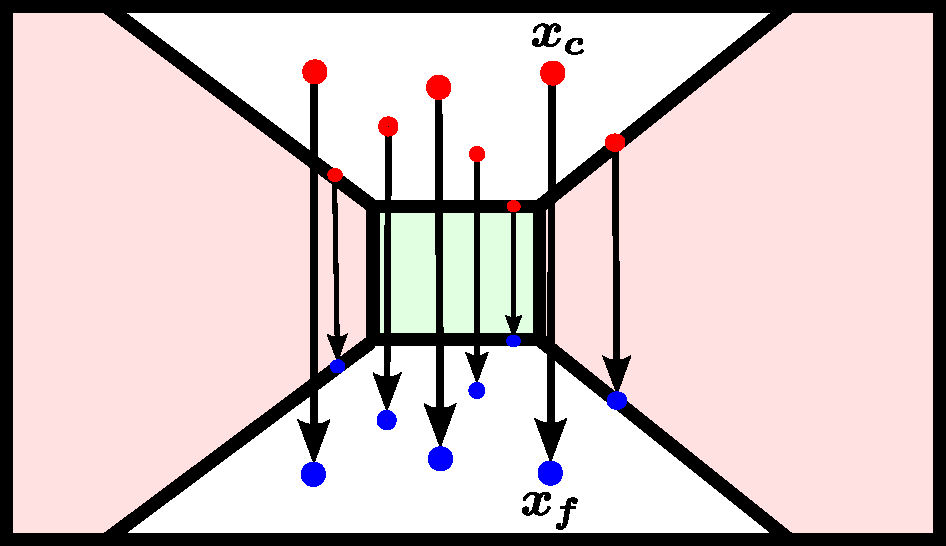
\includegraphics[width=0.5\textwidth]{manhattan_homology}
  \caption{The mapping $\Hcf$ transfers points between the ceiling
    and floor.}
  \label{fig:homology}
\end{figure}

Since the floor and ceiling planes are parallel, there is a planar
homology $\Hcf$ such that
\begin{equation}
  \FloorPt = \Hcf \CeilPt
\end{equation}
if and only if $\pfloor$ and and $\pceil$ are in correspondence
\cite{Criminisi01}. We define $\HomParam$ as the unique real number
such that
\begin{equation}
  \label{eq:manhattanhom}
  \Hcf = I + \HomParam\frac{\vvpt\horizon^T}{\vvpt \cdot \horizon}
\end{equation}
where
\begin{equation}
  \horizon = \CamMatrix\CamR\ex \cross \CamMatrix\CamR\ey
\end{equation}
is the horizon line. Given any corresponding pair
$(\FloorPt,\CeilPt)$, $\HomParam$ is given by \cite{Criminisi01}
\begin{equation}
  \HomParam = 
  \langle\vvpt,\CeilPt,\FloorPt,(\CeilPt\times\FloorPt)\times\horizon\rangle ~,
\end{equation}
where
\begin{equation}
  \langle \vect{a},\vect{b},\vect{c},\vect{d} \rangle = \frac{
    (\vect{a}-\vect{c}) \cdot (\vect{b}-\vect{d})
  }{
    (\vect{b}-\vect{c}) \cdot (\vect{a}-\vect{d})
  }
\end{equation}
is the characteristic cross ratio of $\Hcf$.

\changedsinceviva{
Note that $\HomParam$ is invariant to the camera intrinsics since the
cross ratio is a projective invariant\cite{Criminisi01}. We therefore
assume without loss of generality that $\CamMatrix$ is the identity
for the remainder of this section.
}

To complete our parametrisation of the floor and ceiling planes we
need to show how to compute $(\HomParam,\ScaleParam)$ from
$(\zfloor,\zceil)$. We may simply set $\ScaleParam$ to either
$\zfloor$ or $\zceil$. Let
\begin{eqnarray}
  \efloor = \zfloor ~ \ez \\
  \eceil = \zceil ~ \ez \\
  \pfloor = \RetProj{\efloor} \\
  \pceil = \RetProj{\eceil}
\end{eqnarray}
Then
\begin{eqnarray}
  (\pceil \cross \pfloor) \cross \horizon &=&
    \bigl((\RetProj{\efloor}) \cross (\RetProj{\eceil}\bigr))
    \cross
    \bigl(\CamR\ex \cross
          \CamR\ey \bigr)\\
  &=& \bigl( (\RetProj{\eceil}) \cross (\RetProj{\efloor}) \bigr)
      \cross
      \CamR(\ex\cross\ey) \\
  &=& \bigl( \CamR(\eceil-\efloor)\cross\CamTr \bigr)
      \cross
      \CamR\ez ~.
\end{eqnarray}
We can now write
\begin{eqnarray}
  \HomParam &=& 
    \langle\vvpt,\pceil,\pfloor,(\pceil\cross\pfloor)\cross\horizon\rangle \\
  &=& \frac{
    \bigl(\vvpt-\pfloor\bigr)^T
    \bigl(\pceil-(\pceil\cross\pfloor)\cross\horizon\bigr)
   }{
    \bigl(\pceil-\pfloor\bigr)^T
    \bigl(\vvpt-(\pceil\cross\pfloor)\cross\horizon\bigr)
   }\\
  &=& \frac{
    \bigl(\CamR\ez - (\CamR\efloor+\CamTr)\bigr)^T
    \bigl(\CamR\eceil+\CamTr-
          (\CamR(\eceil-\efloor)\cross\CamTr)\cross\CamR\ez
          \bigr)
   }{
    \bigl(\CamR\eceil+\CamTr-\CamR\efloor-\CamTr\bigr)^T
    \bigl(\CamR\ez-
          (\CamR(\eceil-\efloor)\cross\CamTr)\cross\CamR\ez
          \bigr)
   }\\
  &=& \frac{
    \bigl(\ez - \efloor - \CamR^T\CamTr\bigr)^T R^T
    \bigl(\CamR\eceil+\CamTr-
          (\CamR(\eceil-\efloor)\cross\CamTr)\cross\CamR\ez
          \bigr)
   }{
    \bigl(\eceil-\efloor\bigr)^T R^T
    \bigl(\CamR\ez-
          (\CamR(\eceil-\efloor)\cross\CamTr)\cross\CamR\ez
          \bigr)
   }\\
  &=& \frac{
    \bigl(\ez - \efloor - \CamR^T\CamTr\bigr)^T
    \bigl(\eceil + \CamR^T\CamTr -
          ((\eceil-\efloor)\cross\CamR^T\CamTr)\cross\ez
          \bigr)
   }{
    (\eceil-\efloor)^T\ez -
    (\eceil-\efloor)^T(((\eceil-\efloor)\CamR^T\CamTr)\ez)
   }\\
  &=& \frac{
    (\ez-\efloor-\CamR^T\CamTr)^T(\eceil+\CamR^T\CamTr)
    +(\zceil-\zfloor)(\|\CamTr\|^2 - (\ez^T\CamR^T\CamTr)^2)
   }{
    \zceil-\zfloor
   }\\
  &=& \frac{1}{\zceil-\zfloor}
    \Bigl( (\zceil + \zcam)(1-\zfloor-\zcam) + \zcam^2 - \|\CamTr\|^2 \Bigr)
     + \|\CamTr\|^2 - \zcam^2
\end{eqnarray}
where in the last line we substituted $\zcam =
\ez^T\CamR^T\CamTr$.

\subsection{Parametrising walls}

We choose to parametrise $\Polyline$ in image coordinates because this
will simplify the algorithms to be presented later. We first present
the image--domain parametrisation, then show that it uniquely
specifies a 3D scene.

Consider the scenes shown in \figref{example-scenes}. Following
rectification, vertical edges in the world appear vertical in each
image, including the vertical seams between adjacent wall segments, so
any line drawn vertically from the top to bottom of a rectified image
intersects exactly one wall segment. That this is true in general
follows from our assumption that walls meet at vertical seams and
extend continuously from floor to ceiling, that the camera is located
between the floor and ceiling planes, and that the environment is
closed.

\begin{figure}[tb]%
  \centering
    \begin{tabular}{ccc}
      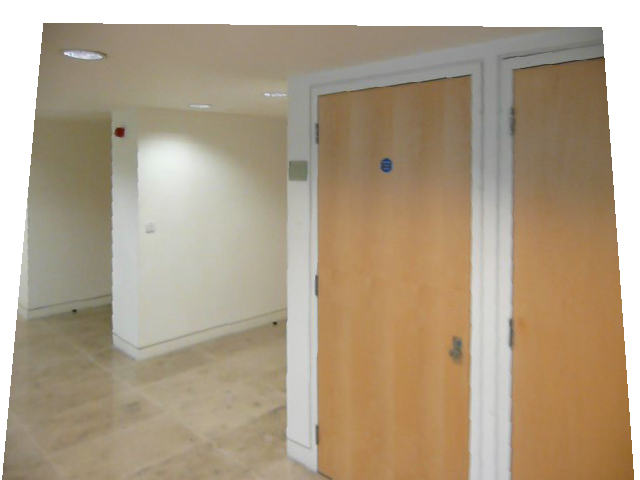
\includegraphics[width=0.3\textwidth]{true_models/lab_ground1_010_rect.png} &
      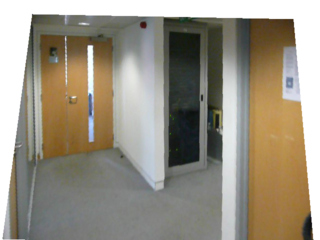
\includegraphics[width=0.3\textwidth]{true_models/lab_kitchen_030_rect.png} &
      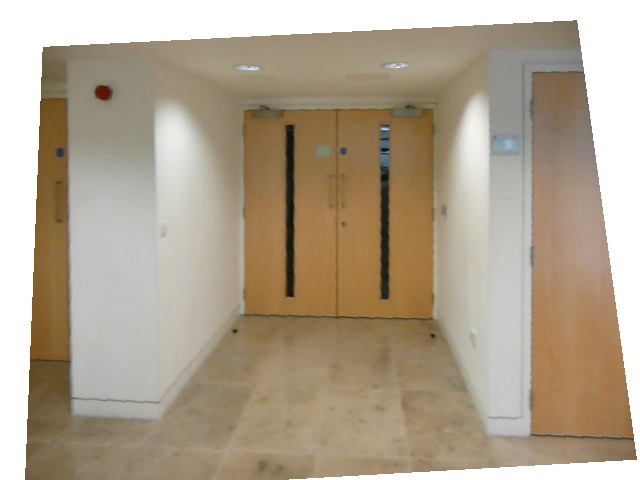
\includegraphics[width=0.3\textwidth]{true_models/lab_ground1_030_rect.png}
      \\      
      \includegraphics[width=0.3\textwidth]{true_models/lab_ground1_010} &
      \includegraphics[width=0.3\textwidth]{true_models/lab_kitchen_030} &
      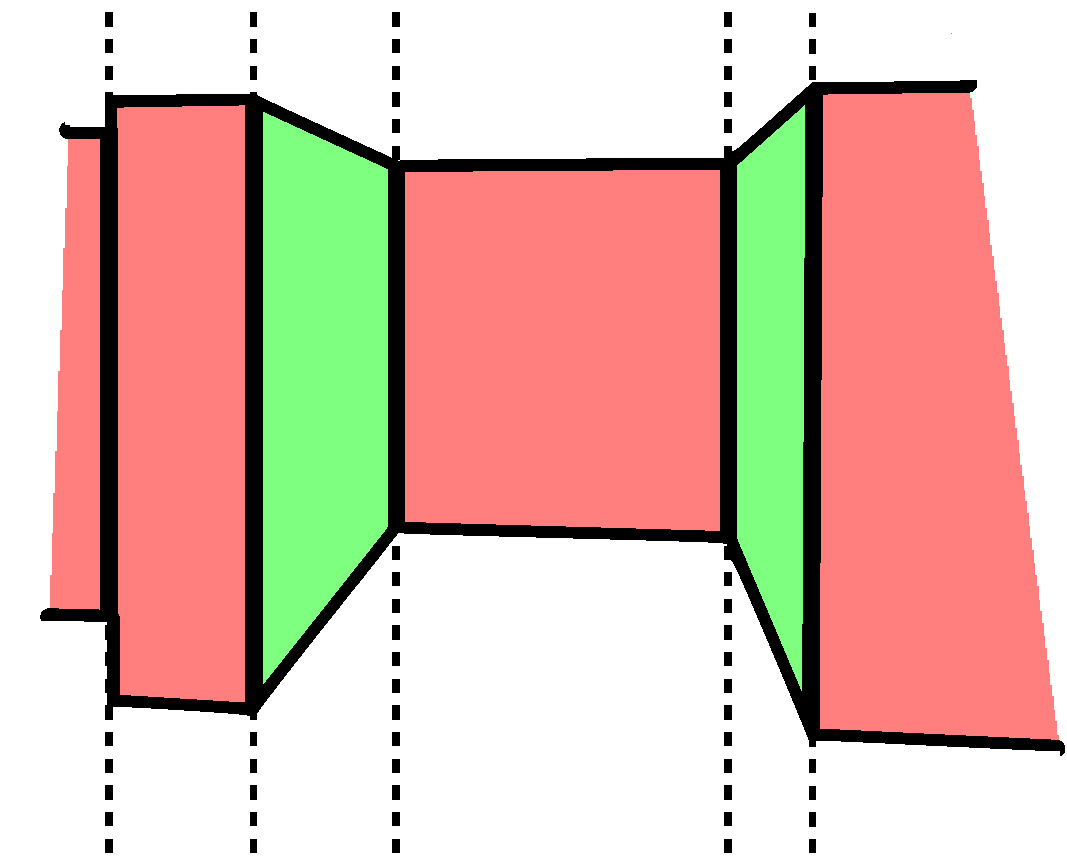
\includegraphics[width=0.3\textwidth]{true_models/lab_ground1_030}
    \end{tabular}
  \caption{Three input images and the indoor Manhattan models we
    seek. Notice how each image column intersects exactly one
    wall.}
  \label{fig:example-scenes}
\end{figure}

\changedsinceviva{
It turns out that once the vanishing points $\vpt_i$ and the Manhattan
homology $\Hcf$ are known, the quadrangle outlining a wall segment in
rectified image coordinates is fully specified by just four variables
(one binary and three scalars) 
}
\begin{equation}
  \label{eq:wall-def}
  \Wall = ( x_0, y, \WallOrient, x_1 )
\end{equation}
as illustrated in \figref{pqrs}. $x_0$ is the location of the left
edge, $x_1$ is the location of the right edge, $y$ is the
$y$--coordinate of the top--left corner, and $\WallOrient\in\{1,2\}$
is the index of the vanishing point associated with the wall. \changedsinceviva{The four
vertices of the wall are then given by}
\begin{eqnarray}
  \label{eq:pi}
  \vect{p_i} &=& \begin{bmatrix}x&y&1\end{bmatrix}^T \\
  \label{eq:qi}
  \vect{q_i} &=& \vect{p_i}\cross\vect{v_{\WallOrient_i}}\cross
               \begin{bmatrix}1&0&-x_{i+1}\end{bmatrix}^T\\
  \label{eq:ri}
  \vect{r_i} &=& \Hcf \vect{q_i}\\
  \label{eq:si}
  \vect{s_i} &=& \Hcf \vect{p_i} ~.
\end{eqnarray}

\begin{figure}[tb]%
  \centering
  \quad
  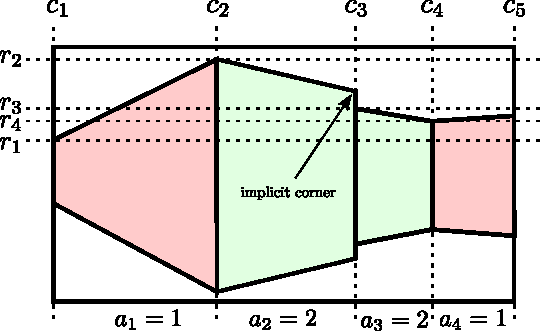
\includegraphics[width=0.5\textwidth]{new-pqrs}
  \caption{The scalars $x_i,x_{i+1},y_i,$ together with the
    vanishing point index $\WallOrient_i\in\{1,2\}$ and the homology $\Hcf$
    fully determine the four vertices of a wall.}
  \label{fig:pqrs}
\end{figure}

Since each image column intersects exactly one wall, we may think of
the scene as a sequence of walls from left to right in the image. This
observation suggests our scene parametrisation, which is simply a
sequence of wall segments (see \figref{vertex-representation}. We make
the additional observation that the right edge of a wall ($x_1$ in
equation \eqnref{wall-def}) is redundant because it is always
coincident with the left edge of the wall to its right. \changedsinceviva{A scene
therefore is fully specified by }
\begin{equation}
  \Scene =
  ( x_1,y_1,\WallOrient_1,
  ~x_2,y_2,\WallOrient_2,
  ~\ldots,
  ~x_{n-1},y_{n-1},\WallOrient_{n-1},
  ~x_n ) ~.
  \label{eq:vertex-repr}
\end{equation}
\changedsinceviva{These values are illustrated in
\figref{vertex-representation}}. Note that although
the right edge of a wall always coincides with the left edge of its
neighbour, it is not always the case that the top and bottom edges of
adjacent walls meet at a point, \ie $\vect{r_i} \neq \vect{s_{i+1}}$
in general. \changedsinceviva{For example, notice the second wall in
\figref{vertex-representation}}.

\begin{figure}[tb]
  \centering
  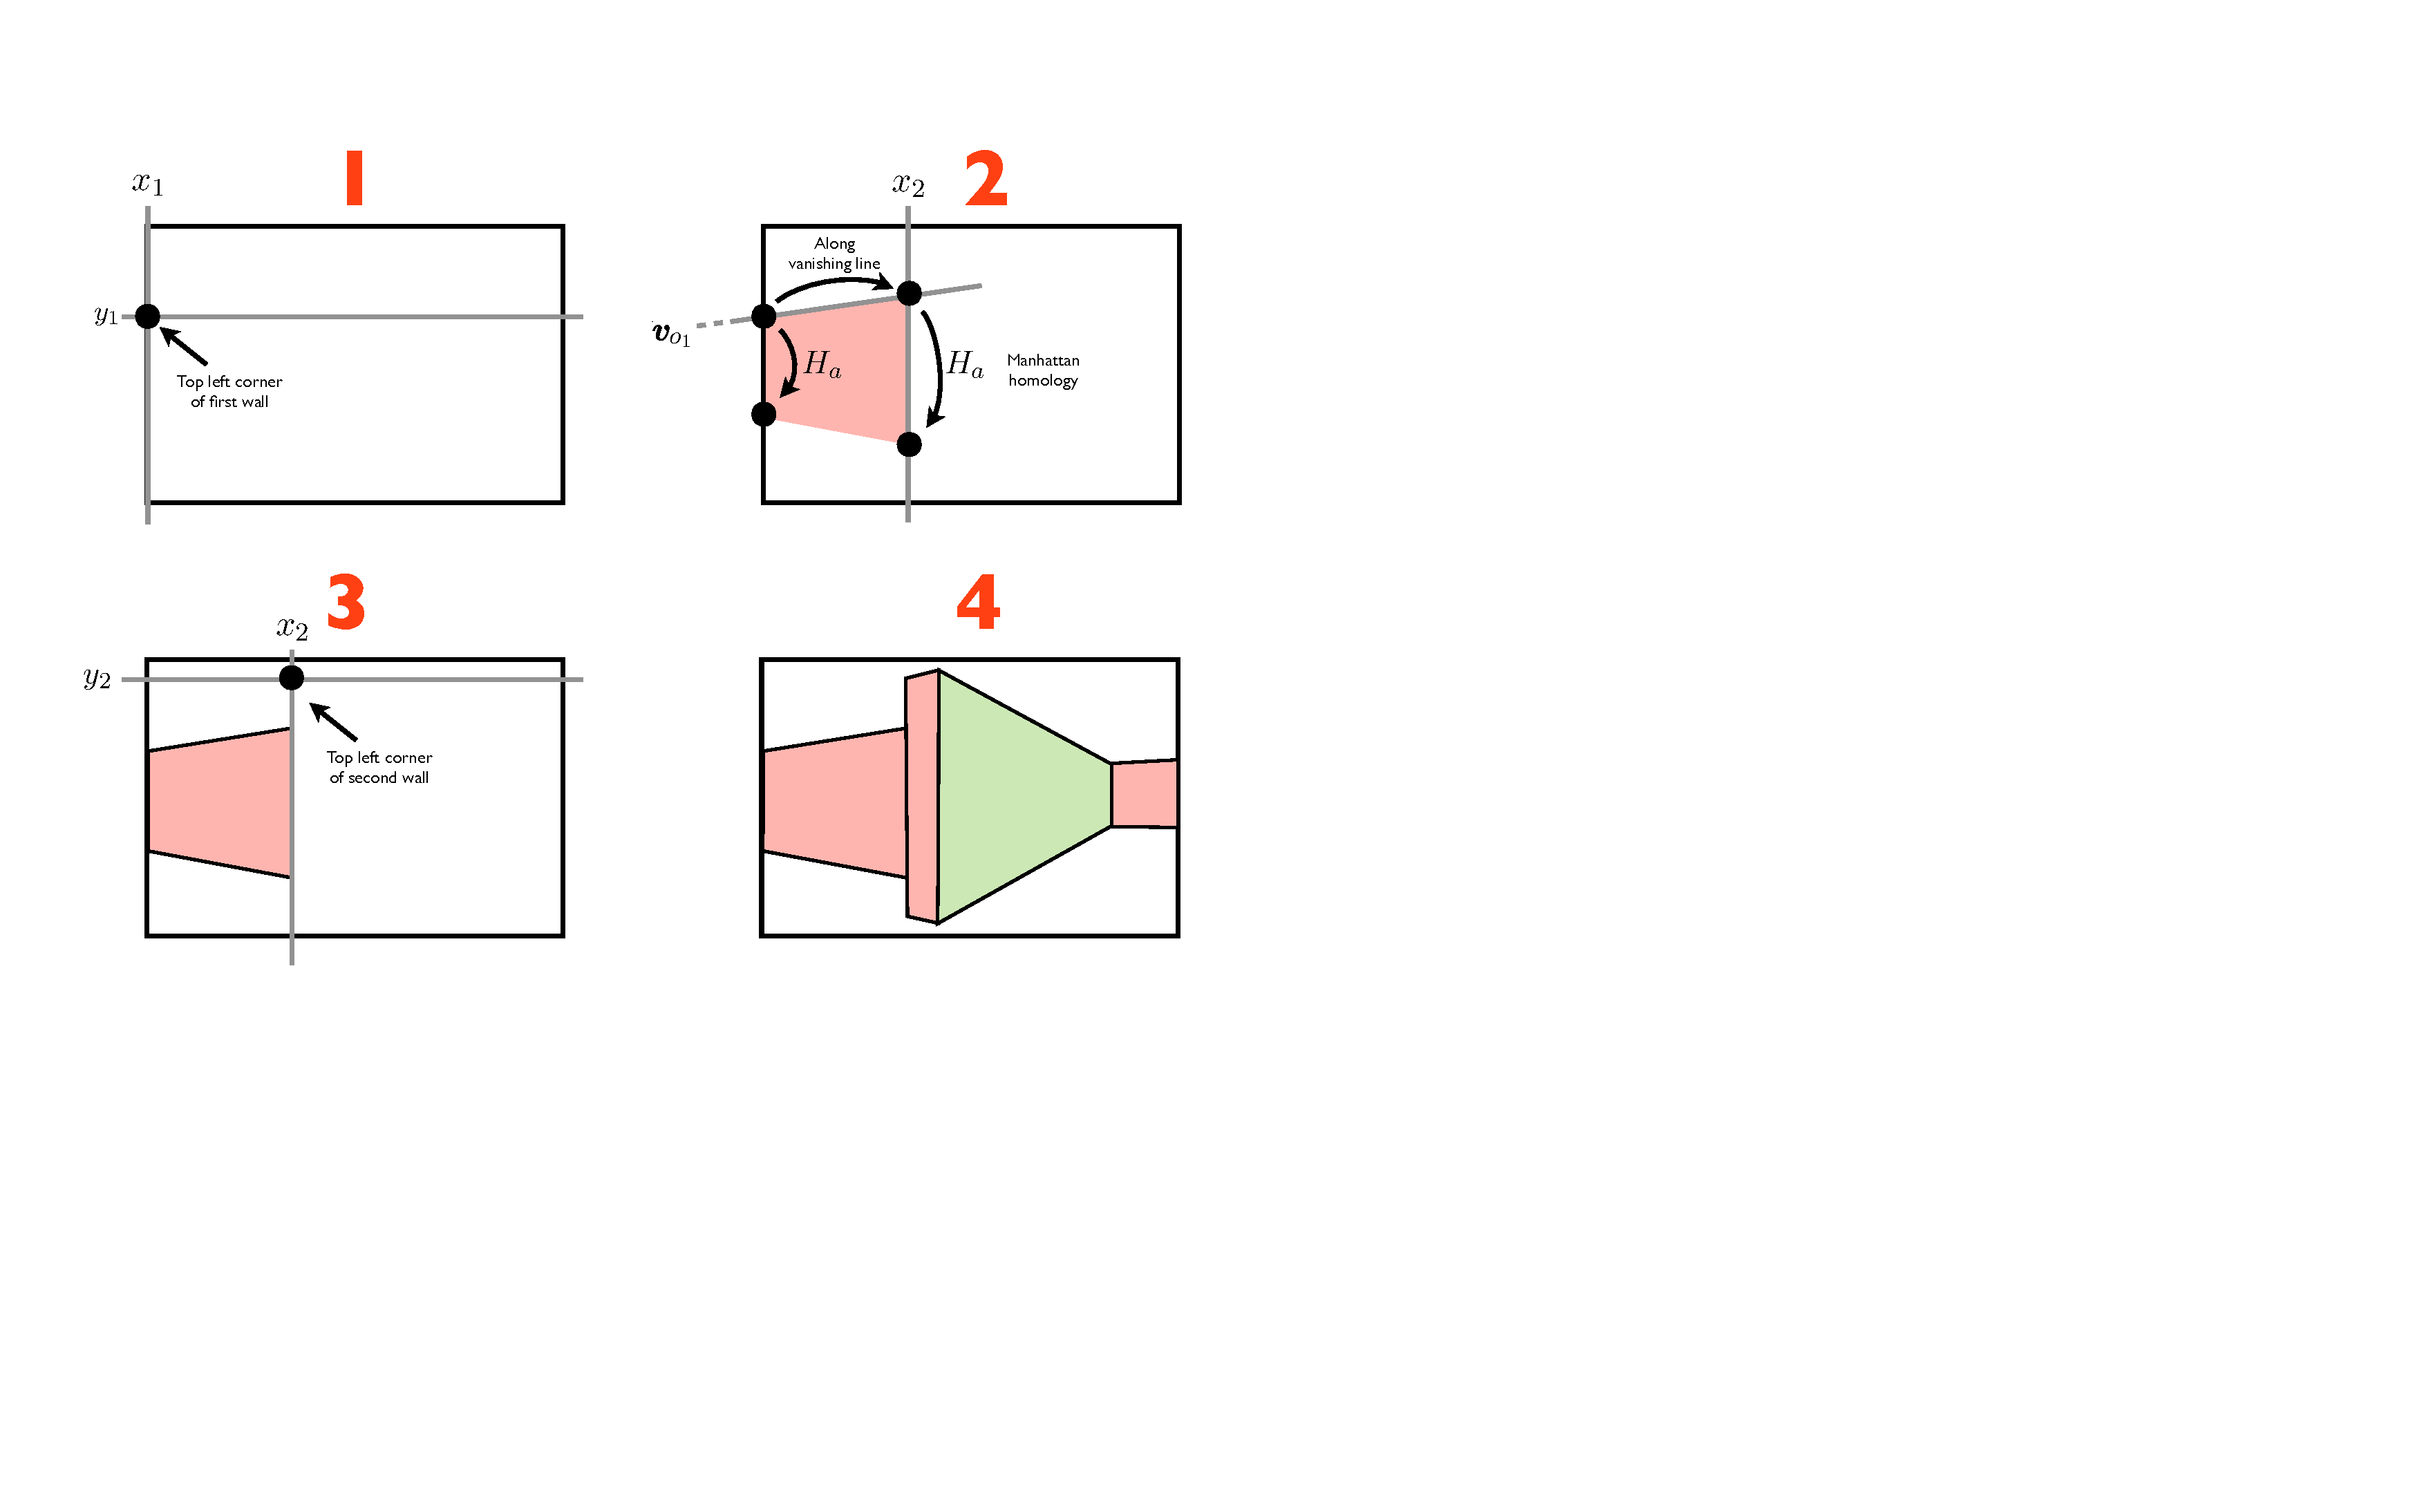
\includegraphics[width=\textwidth]{vertex-representation}
  \caption{\changedsinceviva{The meaning of the parameters in the
      vertex representation is illustrated through a constructive
      example. (1) The top--left corner of the first wall is at
      $(x_1,y_1)$. (2) The top--right corner of the first wall is
      found by intersecting the vanishing line with the line
      $x_2$. Then both points are projected through $\Hcf$, yielding
      the four corners of the first wall. (3) The top--left corner of
      the second wall is at $(x_2,y_2)$. (4) This is repeated to build
      up the entire model.}}
  \label{fig:vertex-representation}
\end{figure}

\subsubsection{Physical Feasibility}

Not all scenes $\Scene$ are physically realisable
as metric reconstructions, but those that are not can be discarded
using simple tests on the locations of walls and vanishing points as
enumerated by Lee \etal \cite{Lee09}. The reader is referred to their
paper for details; the key result for our purposes is that a model is
feasible if all of its corners are feasible, and the feasibility of a
corner is dependent only on the immediately adjoining walls. We
discuss these issues in detail during \chapref{inference}.

\subsection{The Seam Representation}
\label{sec:seam-representation}

\begin{figure}[tb]%
  \centering
  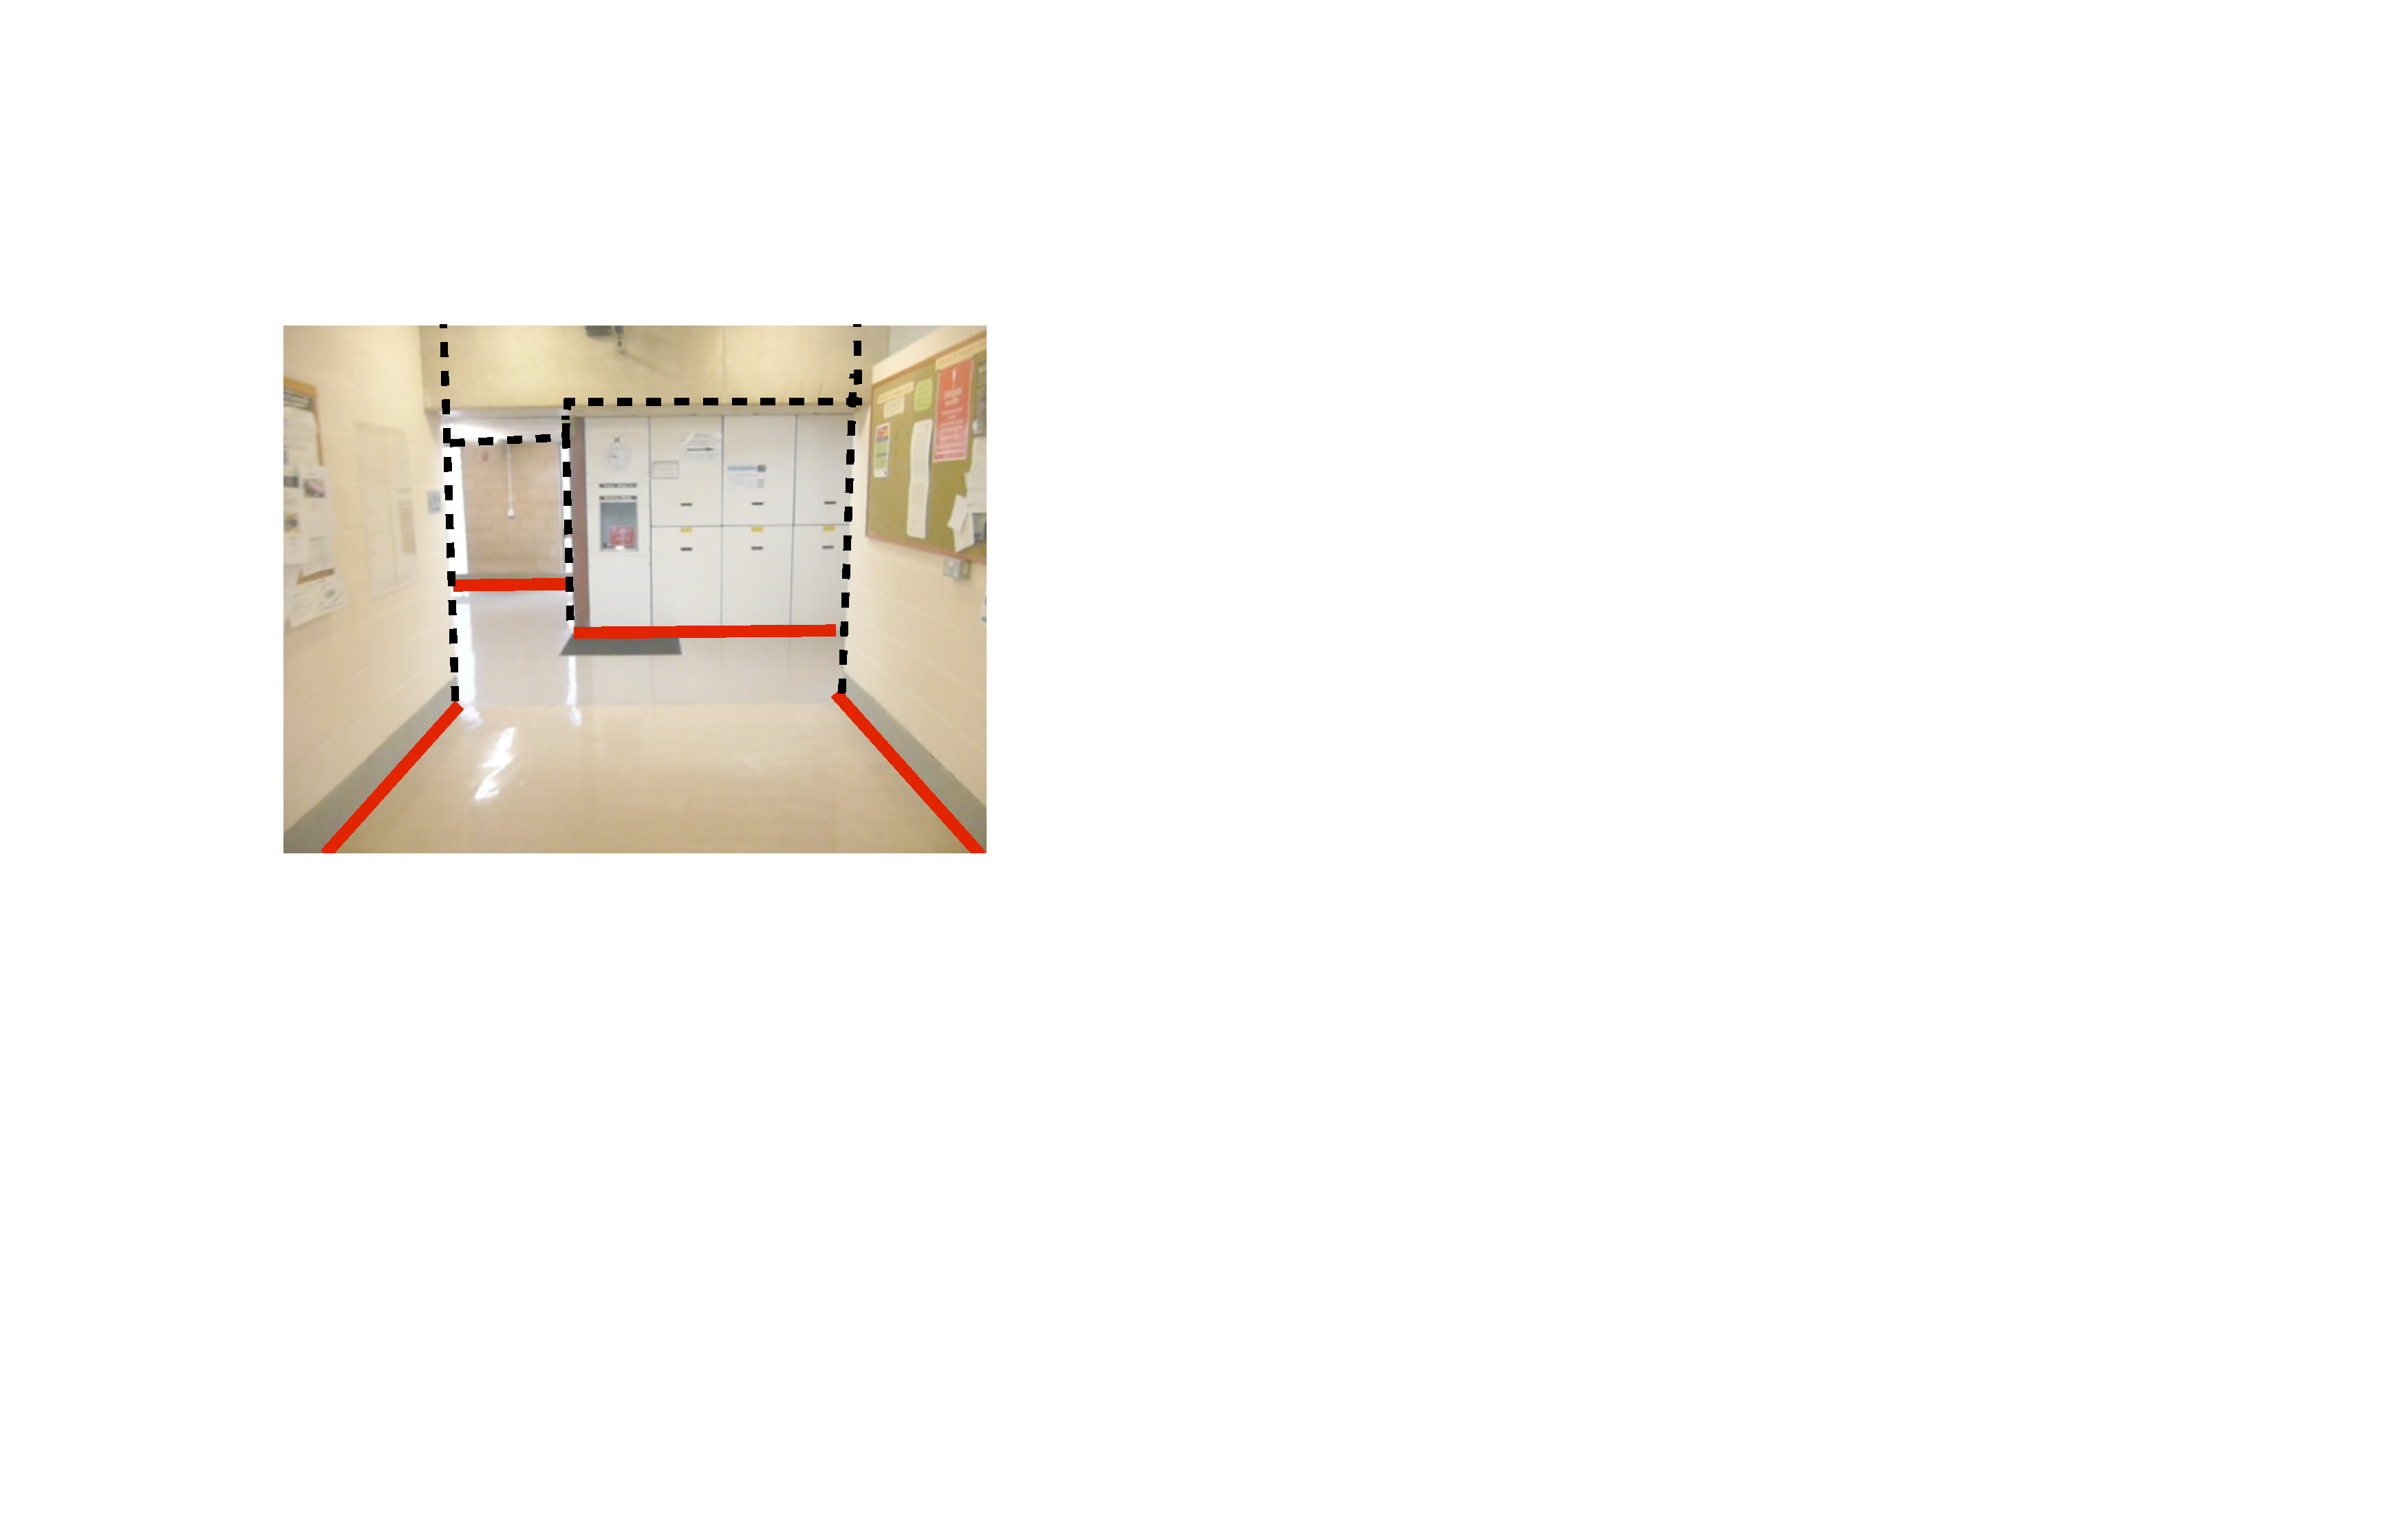
\includegraphics[width=0.6\textwidth]{seam-representation}
  \caption{\changedsinceviva{An example of an indoor Manhattan scene and its seam
    representation shown in red. The black dotted lines can be
    recovered from the seam using the Manhattan homology $\Hcf$.}}
  \label{fig:seam-example}
\end{figure}

For the purpose of the probabilistic model that we will present in
chapter \chapref{inference} we will now present an additional, slightly
different parametrisation that we will refer to as the \textit{seam}
representation of indoor Manhattan scenes. We will refer to the
parametrisation of equation \eqnref{vertex-repr} as the
\textit{vertex} representation. A scene in vertex representation
$\Scene$ uniquely determines a scene in seam $\Seam$ representation,
but the converse is not true. For this reason we will always work in
the vertex representation during inference, but to evaluate
likelihoods, priors, and posteriors for a fixed scene we will find it
notationally more convenient to work in the seam representation. Under
the seam representation a scene is represented by associating a pair of
scalars $(\seam_j,\WallOrient_j)$ to each image column $j$,
\begin{equation}
  \label{eq:seam-def}
  \Seam = \{(\seam_j,\WallOrient_j)\}_{j=0}^\Width  ~,
\end{equation}
where $\seam_j$ is the $y$--coordinate of the bottom edge of the wall
that intersects the $j$\th column, and $\WallOrient_j\in\{1,2\}$ is
the index of its associated vanishing point. Note that the size of
this representation is proportional to the image width, whereas the
size of the vertex representation is proportional to the number of
distinct wall segments. See \figref{seam-example}
for an illustration of this parametrisation.

We compute the seam representation $\Seam$ from a scene in vertex
representation $\Scene$ as follows. For each $j\in[0,\Width]$ we
identify the index of the (unique) wall segment that intersects column
$j$ by finding $x_i,x_{i+1}\in\Scene$ such that $x_i \leq j \leq
x_{i+1}$. Next we compute $\vect{s_i}$ and $\vect{r_i}$ according to
equations \eqnref{si} and \eqnref{ri}, after which the position of the
wall seam at column $j$ is given by
\begin{equation}
  \label{eq:seam-from-scene}
  \seam_j = (\vect{r_i} \cross \vect{s_i}) \cross
  \begin{bmatrix} 0 & 1 & -j \end{bmatrix}^T ~.
\end{equation}
Finally, the orientation $\WallOrient_j$ at column $j$ is equal to the
orientation of the identified wall segment, $\WallOrient_i$. The
constructive process described above shows that there is exactly one
seam $\Seam$ associated with a scene in vertex
representation. However, there is no unique mapping in the reverse
direction. In other words, the mapping from vertex representation to
seam representation is many--to--one.

%%%%%%%%%%%%%%%%%%%%%%%%%%%%%%%%%%%%%%%%%%%%%%%%%%%%%%%%%%%%%%%%%%%%%%%%
\section{Deductions}
\label{sec:misc-geometry}

In this section we make several geometric observations that are
crucial to the following chapters.

\subsection{Classification of Corners}
\label{sec:corner-categories}

\begin{figure}[tb]%
  \centering
  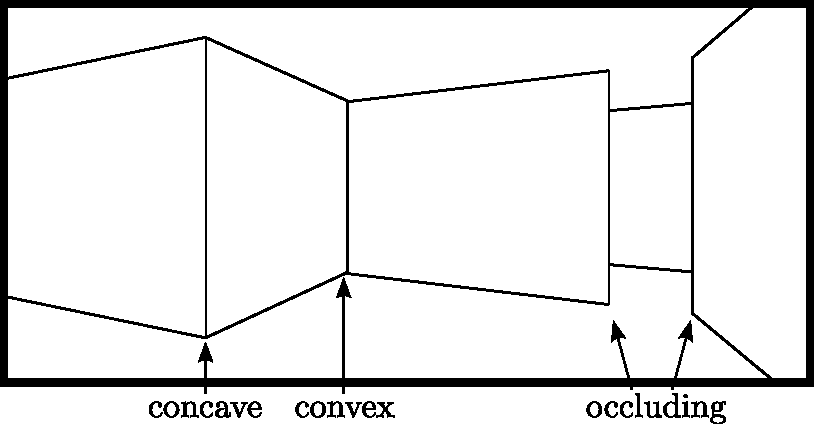
\includegraphics[width=0.6\textwidth]{corner-types}
  \caption{Each corner in an indoor Manhattan environment can be
    categorised as concave, convex, or occluding.}
  \label{fig:corner-types}
\end{figure}

Lee \etal \cite{Lee09} showed that corners between adjacent walls
can be divided into three categories as follows.
\begin{itemize}
  \item{A \textit{convex corner} occurs where two wall segments meet
    exactly and form an internal angle not greater than $180\degrees$, \ie
    \begin{eqnarray}
      \vect{r_i} &=& \vect{s_{i+1}}\\
      &\mbox{and}&\\
      \frac{(\vect{s_i}-\vect{r_i})\cdot(\vect{q_i}-\vect{r_i})}
           {\|\vect{s_i}-\vect{r_i})\|\|(\vect{q_i}-\vect{r_i}\|}
      &\leq&
      \frac{(\vect{r_{i+1}}-\vect{r_i})\cdot(\vect{q_i}-\vect{r_i})}
           {\|\vect{r_{i+1}}-\vect{r_i})\|\|(\vect{q_i}-\vect{r_i}\|} ~.
    \end{eqnarray}
  }
  \item{A \textit{concave corner} occurs where two wall segments meet
    exactly and form an internal angle greater than $180\degrees$, \ie
    \begin{eqnarray}
      \vect{r_i} &=& \vect{s_{i+1}}\\
      &\mbox{and}&\\
      \frac{(\vect{s_i}-\vect{r_i})\cdot(\vect{q_i}-\vect{r_i})}
           {\|\vect{s_i}-\vect{r_i})\|\|(\vect{q_i}-\vect{r_i}\|}
      &>&
      \frac{(\vect{r_{i+1}}-\vect{r_i})\cdot(\vect{q_i}-\vect{r_i})}
           {\|\vect{r_{i+1}}-\vect{r_i})\|\|(\vect{q_i}-\vect{r_i}\|} ~.
    \end{eqnarray}
  }
  \item{An \textit{occluding corner} occurs where two wall segments
    meet but their lower edges do not coincide, \ie
    \begin{equation}
      \vect{r_i} \neq \vect{s_{i+1}}
    \end{equation}
  }
\end{itemize}
Examples of each type of corner are shown in \figref{corner-types}.

\subsection{Recovering Metric Scene Structure}
\label{sec:metric-recovery}

We now show that once $\SceneR$ and $\Zs$ are known, a scene $\Scene$
in vertex representation uniquely specifies a 3D model. We show this
by demonstrating how to convert a scene $\Scene$ to a floorplan
$\Floorplan$, after which we may apply equations \eqnref{pi},
\eqnref{qi}, \eqnref{ri}, and \eqnref{si} to recover a polygonal
reconstruction. In the single image context, the reconstruction is
recovered up to scale (there is only a one--parameter scale
ambiguity since cameras are assumed calibrated and vanishing
directions are assumed mutually orthogonal). \changedsinceviva{In the context of multiple
views the reconstruction is recovered within the coordinate system in
which the camera poses are given to us (which is typically the
coordinate system identified by structure--from--motion).
}

Let $\backproj(\Pixel;\vect{w},\CamMatrix,\CamR,\CamTr)$ be the
back--projection of image point $\Pixel$ onto the plane
$\vect{x}\cdot\vect{w}=0$ given camera intrinsics $\CamMatrix$ and
extrinsics $\CamR,\CamTr$. To compute this we solve for $\vect{y}$ in
\begin{equation}
  P \vect{y} = \vect{0}
\end{equation}
where
\begin{equation}
  P =
  \begin{bmatrix}
    & \CamMatrix\CamR & & \CamMatrix\CamTr-\Pixel \\
    0 & 0 & 1 & -\zfloor
  \end{bmatrix}~.
\end{equation}
We will usually omit the camera parameters and simply write
$\backproj(\Pixel;\vect{w})$. Furthermore, since we will often be
back--projecting onto planes orthogonal to the $z$ axis we adopt the
short--hand
\begin{equation}
  \backproj(\Pixel;z) = \backproj(\Pixel;
    \begin{bmatrix}0 & 0 & 1 & -z\end{bmatrix}) ~.
\end{equation}

To recover a floorplan $\Floorplan$ from a scene $\Scene$ we simply
need to back--project $\vect{q_i},\vect{s_i}$ pairs onto the floor
plane. This is formalised in \algref{scene-to-recon}.

\begin{algorithm}
  \begin{algorithmic}
    \REQUIRE{$\Scene =(x_1,y_1,\WallOrient_1,\ldots,x_n)$ ~~~
      \{a scene in vertex representation\}}
    \ENSURE $\Floorplan=\{(\vect{u_i},\vect{v_i})\}$
    \STATE{$\Floorplan \leftarrow \emptyset$}
    \FOR{$i=1 \ldots n-1$}
      \STATE{$\vect{u_i}=\backproj(\vect{s_i}; \zfloor)$}
      \STATE{$\vect{u_i}=\backproj(\vect{r_i}; \zfloor)$}
      \STATE{$\Floorplan \leftarrow \Floorplan \union (\vect{u_i},\vect{v_i})$}
    \ENDFOR
  \end{algorithmic}
  \caption{\label{alg:scene-to-recon}
    Recovering a metric 3D scene from the vertex representation
    $\Scene$.}
\end{algorithm}

\subsection{Recovering Orientation and Depth}
We say that an indoor Manhattan scene $\Scene$ predicts the depth
$\Depth_{\Pixel}$ of each pixel $\Pixel$ because we can compute the
depth of each $\Pixel$ given the hypothesis $\Scene$. \changedsinceviva{All depths are
recovered within the coordinate system given to us by
structure--from--motion}. Similarly, a
scene predicts an orientation $\Orient_{\Pixel}\in\SetOfOrients$ for
each pixel, which is the orientation of the 3D surface that
projects to $\Pixel$.

To compute either the orientation $\Orient_{\Pixel}$ or depth
$\Depth_{\Pixel}$ for an image point $\Pixel$ we first need to
identify a wall that contains $\Pixel$ within its (image--domain)
outline. If there is such a wall then $\Pixel$ has the orientation of
that wall and we back--project $\Pixel$ onto the wall in 3D to recover
depth. If $\Pixel$ is not contained by any wall then $\Pixel$ must be
on the floor or ceiling and therefore has the horizontal
orientation. In this case we recover depth by back--projecting onto
the floor or ceiling plane, according to whether $\Pixel$ is above or
below the horizon respectively. This process is formalised in
\algref{computing-from-scene}.

\begin{algorithm}[tb]
  \begin{algorithmic}
    \REQUIRE{$\Scene =(x_1,y_1,\WallOrient_1,\ldots,x_n)$ ~~~ 
       \{a scene in vertex representation\}}
    \REQUIRE $\Pixel=(x,y)\in\Rtwo$
    \REQUIRE $x_1 \leq x < x_n$
    \ENSURE{$i_{\Pixel} \in [1,n],
      \Orient_{\Pixel} \in \SetOfOrients,
      \Depth_{\Pixel}>0$}
    \FOR{$i = 1 \ldots n-1$}
      \IF{$x_i \leq x < x_{i+1}$}
        \STATE\COMMENT{Compute the floor--wall and ceiling--wall
          seam in column $x$}
          % TODO: euclidean projection needed below!!
        \STATE{$\seam_f \leftarrow \ey \cdot (\vect{s_i}
          \cross \vect{r_i})
          \cross \begin{bmatrix}1&0&-x\end{bmatrix}^T$}
        \STATE{$\seam_c \leftarrow \ey \cdot (\vect{s_i}
          \cross \vect{r_i})
          \cross \begin{bmatrix}1&0&-x\end{bmatrix}^T$}
        \IF{$y < \seam_c$}
          \STATE{$\Orient_{\Pixel} \leftarrow ``vert orient''$}
          \STATE{$X_{\Pixel} \leftarrow \backproj(\Pixel; \zceil)$}
        \ELSIF{$\seam_c < y < \seam_f$}
          \STATE{$\Orient_{\Pixel} \leftarrow \WallOrient_x$}
          \STATE{$w_{\Pixel} \leftarrow
            \begin{bmatrix}
              1 & 0 & 0 & -\backproj(\vect{x_f}; \zfloor)\cdot\ex
            \end{bmatrix}^T$}
          \STATE{$X_{\Pixel} \leftarrow \backproj(\Pixel; w_{\Pixel})$}
        \ELSE
          \STATE{$\Orient_{\Pixel} \leftarrow ``vert orient''$}
          \STATE{$X_{\Pixel} \leftarrow \backproj(\Pixel; \zfloor)$}
        \ENDIF
        \STATE{$\Depth_{\Pixel} \leftarrow
          (\CamR X_{\Pixel} + \CamTr) \cdot \ez$}
        \RETURN
      \ENDIF
    \ENDFOR
  \end{algorithmic}
  \caption{\label{alg:computing-from-scene}
    Recovering orientation and depth for an image location
    $\Pixel$ under a scene hypothesis $\Scene$.}
\end{algorithm}

These calculations are considerably simpler in the seam
representation, which is why it proves useful in following
chapters. Suppose we are given a scene in seam representation $\Seam$
and an integer pixel location $\Pixel\in\Ints^2$. We first look up the
the pair $(\seam_j,\WallOrient_j)\in\Seam$ for the column $j$ in which the
pixel $\Pixel$ falls. Denote this pair
$(\seam_x,\WallOrient_x)$. Then the floor--wall seam in column
$x$ is at $\seam_f=\seam_x$ and the ceiling--wall seam
can be recovered using the Manhattan homology. From here the
orientation and depth at $\Pixel$ are obtained using the procedure
shown in \algref{seam-depth-orient}.

\begin{algorithm}[tb]
  \begin{algorithmic}
    \REQUIRE{$\Seam = \{(\seam_j,\WallOrient_j)\}$ ~~~
      \{a scene in seam representation\}}
    \REQUIRE{$\Pixel=(x,y)\in\Ints^2$ ~~~
      \{a query pixel\}}
    \ENSURE{$\Orient_{\Pixel} \in \SetOfOrients,
      \Depth_{\Pixel}>0$}
    \STATE\COMMENT{Compute the floor--wall and ceiling--wall
      seam in column $x$}
    \STATE{$\seam_f \leftarrow \seam_{x}$}
    \STATE{$\vect{x_f} \leftarrow
      \begin{bmatrix}
        x & \seam_f & 1
      \end{bmatrix}^T$}
    \STATE{$\vect{x_c} \leftarrow \Hcf \vect{x_f}$}
    \STATE{$\seam_c \leftarrow \frac{\vect{x_c}\cdot\ey}
      {\vect{x_c}\cdot\ez}$}
    \IF{$y < \seam_c$}
      \STATE{$\Orient_{\Pixel} \leftarrow ``vert orient''$}
      \STATE{$X_{\Pixel} \leftarrow \backproj(\Pixel; \zceil)$}
    \ELSIF{$\seam_c < y < \seam_f$}
      \STATE{$\Orient_{\Pixel} \leftarrow \Orient_x$}
      \STATE{$\vect{w}_{\Pixel} \leftarrow
        \begin{bmatrix}
          1 & 0 & 0 & -\backproj(\vect{x_f}; \zfloor)\cdot\ex
        \end{bmatrix}^T$}
      \STATE{$X_{\Pixel} \leftarrow \backproj(\Pixel; \vect{w}_{\Pixel})$}
    \ELSE
      \STATE{$\Orient_{\Pixel} \leftarrow ``vert orient''$}
      \STATE{$X_{\Pixel} \leftarrow \backproj(\Pixel; \zfloor)$}
    \ENDIF
    \STATE{$\Depth_{\Pixel} \leftarrow
      (\CamR X_{\Pixel} + \CamTr) \cdot \ez$}
  \end{algorithmic}
  \caption{\label{alg:seam-depth-orient}
    Recovering orientation and depth for an
    image location $\Pixel$ under the seam representation $\Seam$.}
\end{algorithm}

\subsection{Column--wise Decomposability}
\label{sec:col-decomposability}

We have so far shown that the vertex representation suffices to
recover metric scene structure up to scale, and that the depth and
orientation predicted for each pixel can be computed directly from
either the vertex or seam representation. One property of particular
significance for the algorithms to be presented in the remainder of
this thesis is that the procedure of \algref{seam-depth-orient} only
requires access to the pair $(\seam_j,\WallOrient_j)$ for the image
column $j$ that contains the query pixel. That is, the depth and
orientation predicted for a pixel $\Pixel$ are functionally
independent of the location of the floor--wall seam in columns other
than the one containing $\Pixel$.

%%%%%%%%%%%%%%%%%%%%%%%%%%%%%%%%%%%%%%%%%%%%%%%%%%%%%%%%%%%%%%%%%%%%%%%%
\section{Conclusion}

We have presented the indoor Manhattan model, in which the world is
represented by floor, ceiling, and wall planes. We have motivated this
model in terms of its salience, compactness, and the simple
parametrisations it permits. The vertex and seam representations are
the primary contributions of this chapter; their specific structure is
crucial to all following chapters. In particular, we will make
repeated use of the decomposability property described in
\secref{col-decomposability}. While this chapter has described the
geometry of ideal indoor Manhattan environments, the system that we
develop in this thesis is not restricted to such sterile conditions;
rather, the model presented in this chapter describes the scene
structure that we seek to recover \textit{despite} clutter and sensor
noise.


%%%%%%%%%%%%%%%%%%%%%%%%%%%%%%%%%%%%%%%%%%%%%%%%%%
%
\def\localpath{RecoveringOrientation}
\graphicspath{{\localpath/figures/}}
\chapter{Identifying Manhattan Orientations}
\label{chap:orientation}
% If you like chapter abstracts ...
%\begin{quote}{\em This chapter describes an application of 

The abstract text is put into Ch\#/ab\#.tex, where
\# is the chapter number.
}\end{quote}
\begin{quote}
  In order to make use of the Manhattan world assumption we must first
  discover the orientation of the Manhattan world with respect to the
  camera. This chapter focuses on estimating a 3D rotation that
  transforms the three cardinal Manhattan orientations onto the $x$,
  $y$, and $z$ axes. In contrast to much previous work, we seek to
  recover this rotation given a sequence of calibrated images, such as
  may be provided by a structure--from--motion or SLAM system. Where
  previous multiple--view approaches have focused on surface normal
  estimates derived from a reconstructed point cloud, we build upon
  ideas from single--view vanishing point detection and cast
  estimation in terms of photometric information. We develop a
  probabilistic model relating observed line segments to the 3D
  rotation we seek, and solve maximum--likelihood inference using an
  Expectation--Maximisation algorithm. Our likelihoods are derived
  from principled error models, and estimation is performed as a
  single optimisation.  We show that our approach substantially
  out--performs a state--of--the--art approach based on surface
  normals, while providing much greater robustness than single--view
  vanishing point estimation.\footnotemark
\end{quote}

\footnotetext{This work was published in part in:

{ \setlength{\parindent}{0pt} 
  \textit{Flint, Mei, Murray, and Reid,} ``Growing Semantically
  Meaningful Models For Visual SLAM'', in \textit{Proceedings of the
    2010 Conference on Computer Vision and Pattern
    Recognition}\cite{Flint10cvpr} 
} 
}

\section{Introduction}

Many man--made environments contain numerous surfaces oriented in
three mutually orthogonal directions. In order to leverage the special
structure of these Manhattan scenes we must identify these three
canonical directions. Since these directions are assumed to be
orthogonal to one another, identifying them is equivalent to finding a
3--dimensional rotation $\SceneR$ that maps them onto the $x$, $y$,
and $z$ axes.

We assume that an estimate of the camera pose for each frame is
available, such as might be provided by a structure--from--motion
system. We will not use any point cloud generated from
structure--from--motion in this chapter. We assume that the provided
camera poses are measured in a fixed but arbitrary coordinate
frame. Determining $\SceneR$ in the context of a single
image is equivalent to detecting vanishing points since three
vanishing points and a calibrated camera are sufficient to recover
$\SceneR$. However, in the multiple view context it makes sense to
estimate $\SceneR$ jointly using all available information, rather
than to merge single--view estimates post--hoc. One view of the
contribution of this chapter is therefore as a generalisation of
vanishing point detection to multiple calibrated views.

We estimate $\SceneR$ using the assumption that a significant number
of the observed line segments correspond to one of three Manhattan
orientations. We present a graphical model relating line segments to
$\SceneR$, then we present an Expectation--Maximisation algorithm for
inference within this model. Our likelihoods are derived from a
well--defined model of image formation, and we optimise jointly with
respect to all line segments in all views in a single
optimisation. Our approach parallels ideas presented in the
context of single--view vanishing point detection, particularly those
of Andrew Zisserman \cite{Hartley04} and Frank Dellaert
\cite{Schindler2004}. Our contribution is a principled way to
incorporate multiple calibrated views into a single optimisation, and
an empirical demonstration that doing so significantly out--performs
both single--view vanishing point estimation and
surface--normal--based estimators.

\section{Background}

Vanishing point detection has a long history in the computer vision
literature, beginning with the seminal work of
Barnard \etal \cite{BARNARD1983}. In this section we survey key
contributions within this literature and discuss their relationship to
our work.

\subsection{Single View Approaches}

Several approaches to single--image vanishing point detection have
been proposed in the literature
\cite{BARNARD1983,Zhang02,Shufelt99}. Common among all such approaches
is the use of line segments as the fundamental observation from which
inference is performed. The vanishing points under consideration are
assumed to generate several associated line segments, all of which
meet at the vanishing point (modulo measurement errors). The
estimation of vanishing points is approached in various ways. The
classic approach due to Barnard \cite{BARNARD1983} was to project
images onto the Gaussian sphere and use the Hough transform to
identify vanishing points. Several authors have proposed similar
voting schemes under different parametrisations of the accumulator
space that improve statistical robustness.

Shufelt \cite{Shufelt99} introduced explicit error models for observed
line segments, but retained the voting--based estimation
strategy. Hartley and Zisserman \cite{Hartley04} first proposed a
generative model relating vanishing point to line segments and cast
maximum likelihood estimation as a non--linear estimation problem. We
make similar modelling assumptions in the present
work. Kanatani \cite{Kanatani93} minimised the algebraic deviation of
vanishing points from observed line segments, which leads to an
efficient linear least--squares solution at the cost of a less precise
error model. Schinder and Dellaert \cite{Schindler2004} laid out an
integrated Bayesian approach to the estimation of multiple vanishing
points.

The approaches discussed thus far estimate vanishing points
independently, using K--means clustering or the expectation
maximisation algorithm to resolve the assignment of line segments to
vanishing points. Coughlan and Yuille \cite{Coughlan99} observed that
under the Manhattan world assumption the three cardinal vanishing
points are mutually orthogonal and hence their locations in the image
plane are highly correlated. Rather than estimating three independent
vanishing points, the authors cast the estimation problems in terms of
Euler angles corresponding to $\SceneR$, resulting in a three--DoF
estimation problem in place of the 6 for independent vanishing point
estimation. Koseck\`{a} and Zhang \cite{Zhang02} showed that the
Manhattan world assumption can be exploited even in the case of an
uncalibrated camera. Their approach used a prior on camera intrinsics
to condition the estimation process, though the estimation of three
vanishing points was not explicitly coupled after this stage.

Denis \etal \cite{Denis2008} took this a step further by
exploiting a prior on the rotation $\SceneR$ learned from training
data. Whereas Coughlan and Yuille used a discretisation of the space
of rotations to identify $\SceneR$, they showed how to exploit the
Manhattan world assumption under the more principled
Expectation--Maximisation approach of Schindler and Dellaert
\cite{Schindler2004}. The M--step in their approach is a non--linear
optimisation over rotations, leveraging the maximum likelihood
reprojection error of Hartley and Zisserman\cite{Hartley04}.

\changedsinceviva{
Sinha \etal \cite{Sinha2008} show how vanishing points in different
views can be optimised jointly with structure and motion inside a
single bundle adjustment. Their approach fixes the
line/vanishing--point associations using multi--hypothesis RANSAC in
individual views. Structure, motion, and vanishing directions are then
optimised jointly while holding the data associations fixed. Our approach
differs from theirs in that (1) we optimise the data association
variables linking lines to vanishing points jointly with the vanishing
point locations; and (2) we do not refine structure and motion using
the vanishing points.
}

Mirzaei and Roumeliotis \cite{Mirzaei2011} showed that
minimising the algebraic error for three mutually orthogonal vanishing
points can be solved globally using a polynomial solver. Their
approach assumes the algebraic error; it is not clear whether the
reprojection error leads to a likelihood that is amenable to a
polynomial solution.

\changedsinceviva{
Bazin \etal \cite{Bazin2012} recently proposed a novel
globally--optimal vanishing point algorithm based on
branch--and--bound. They search over partitions of the observed
line segments, constrained by the requirement that each partition must
be consistent with some vanishing point to a tolerance $\tau$. This
approach is attractive because it is guaranteed to find the global
optimum. The authors optimise an objective function based on the
number of consistent line segments, whereas most previous approaches
optimise a log--likelihood.
}

\subsection{Multiple View Approaches}

The literature concerning vanishing point estimation from multiple
views is sparse, and generally involves non--photometric approaches to
recover $\SceneR$. Furukawa and Curless \cite{Furukawa09} use
multiple--view stereo to recover a dense point cloud, then estimate
$\SceneR$ by clustering surface normals on the unit hemisphere. Werner
and Zisserman \cite{Werner2002} identify vanishing points
independently in several uncalibrated views, then resolve associations
between views using a combinatorial search.

\section{Overview of Proposed Approach}

Reliable vanishing point detection from single images is fundamentally
challenging in environments in which axis--oriented edges are rare, or
in which one or two cardinal orientations have very few associated
edges. Both scenarios are common in video sequences of indoor
environments since the camera often views only a small portion of the
scene. On the other hand, obtaining a dense reconstruction is a
complex and computationally expensive pre--requisite for a
three--parameter estimation problem. Furthermore, the point cloud
provided by on--line structure--from--motion is too sparse to obtain
accurate surface normal estimates.

We overcome these difficulties by reasoning in terms of line
segments and integrating observations from many frames into the
estimation. Since $\SceneR$ is fixed for all frames it makes sense to
leverage all available data during estimation. Whereas previous
approaches often estimate vanishing points as a precursor to
reconstructing camera poses \cite{Zhang02,Werner2002}, we prefer to rely
on the structure--from--motion system to provide camera poses,
then recover vanishing points afterwards. Under this problem setup we
can relate line segments in all views directly to $\SceneR$ and
therefore incorporate all available evidence into a joint
estimation. We show that this is both computationally efficient and
avoids the fragile single--view estimation scenario.

\changedsinceviva{
The structure--from--motion system we have chosen to work with is the
parallel tracking and mapping (PTAM) approach of Klein and Murray
\cite{Klein07}. This approach is suitable for online experiments,
although this comes at the cost of reduced accuracy compared to global
bundle adjustment. Importantly, PTAM can encounter scale and
orientation drift, so the maps it builds may not be perfectly
metric. While our results with this system are promising, we do notice
small vanishing point inconsistencies between frames, which can lead
to errors in our reconstructions. When operating offline, this could
be alleviated by running global bundle adjustment prior to executing
our system.
}

\section{Generative Model}

\begin{figure}[tb]
  \centering
  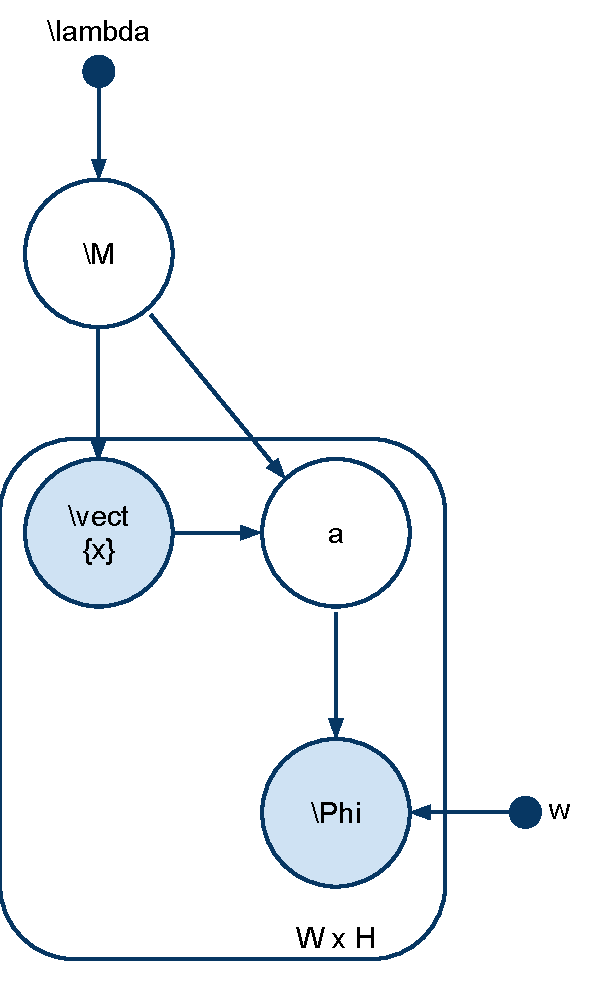
\includegraphics[width=0.5\textwidth]{graphical-model}
  \caption{A graphical model relating line segments to vanishing
    points.}
  \label{fig:R-graphical}
\end{figure}

\begin{figure}[tb]
  \centering
  \subfloat[Error model for line observations.]{
    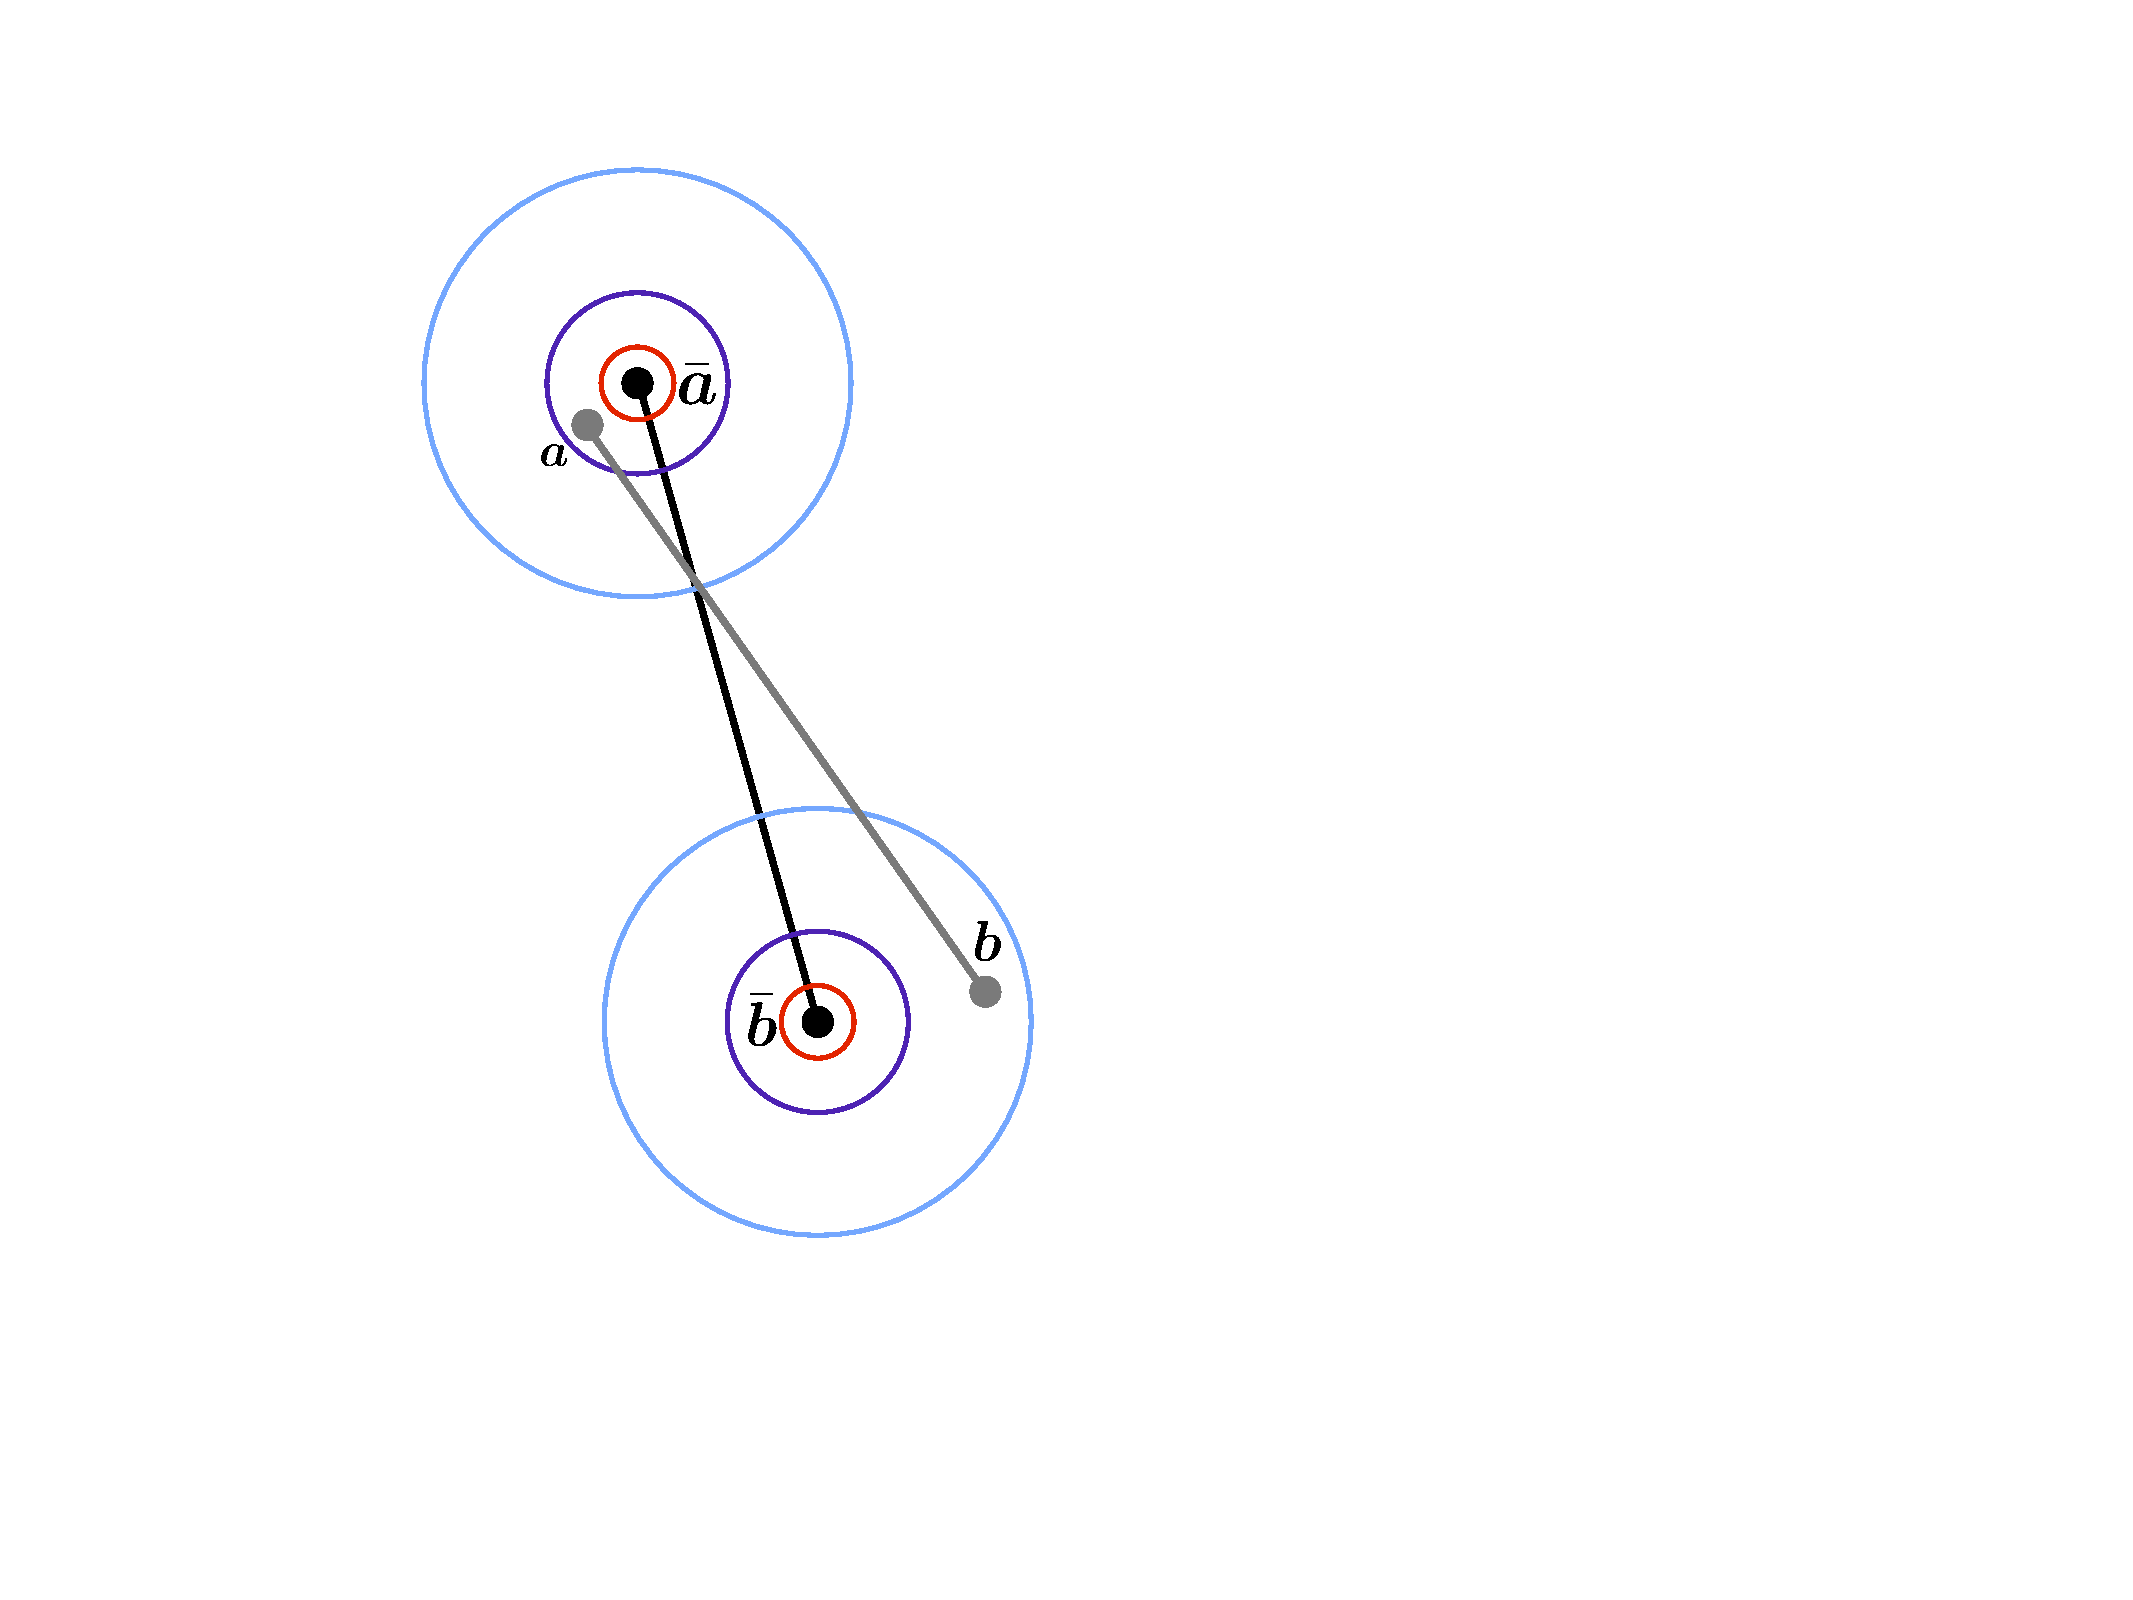
\includegraphics[width=0.4\textwidth]{error-model}
  }
  \qquad
  \subfloat[The reprojection error, $d$.]{
    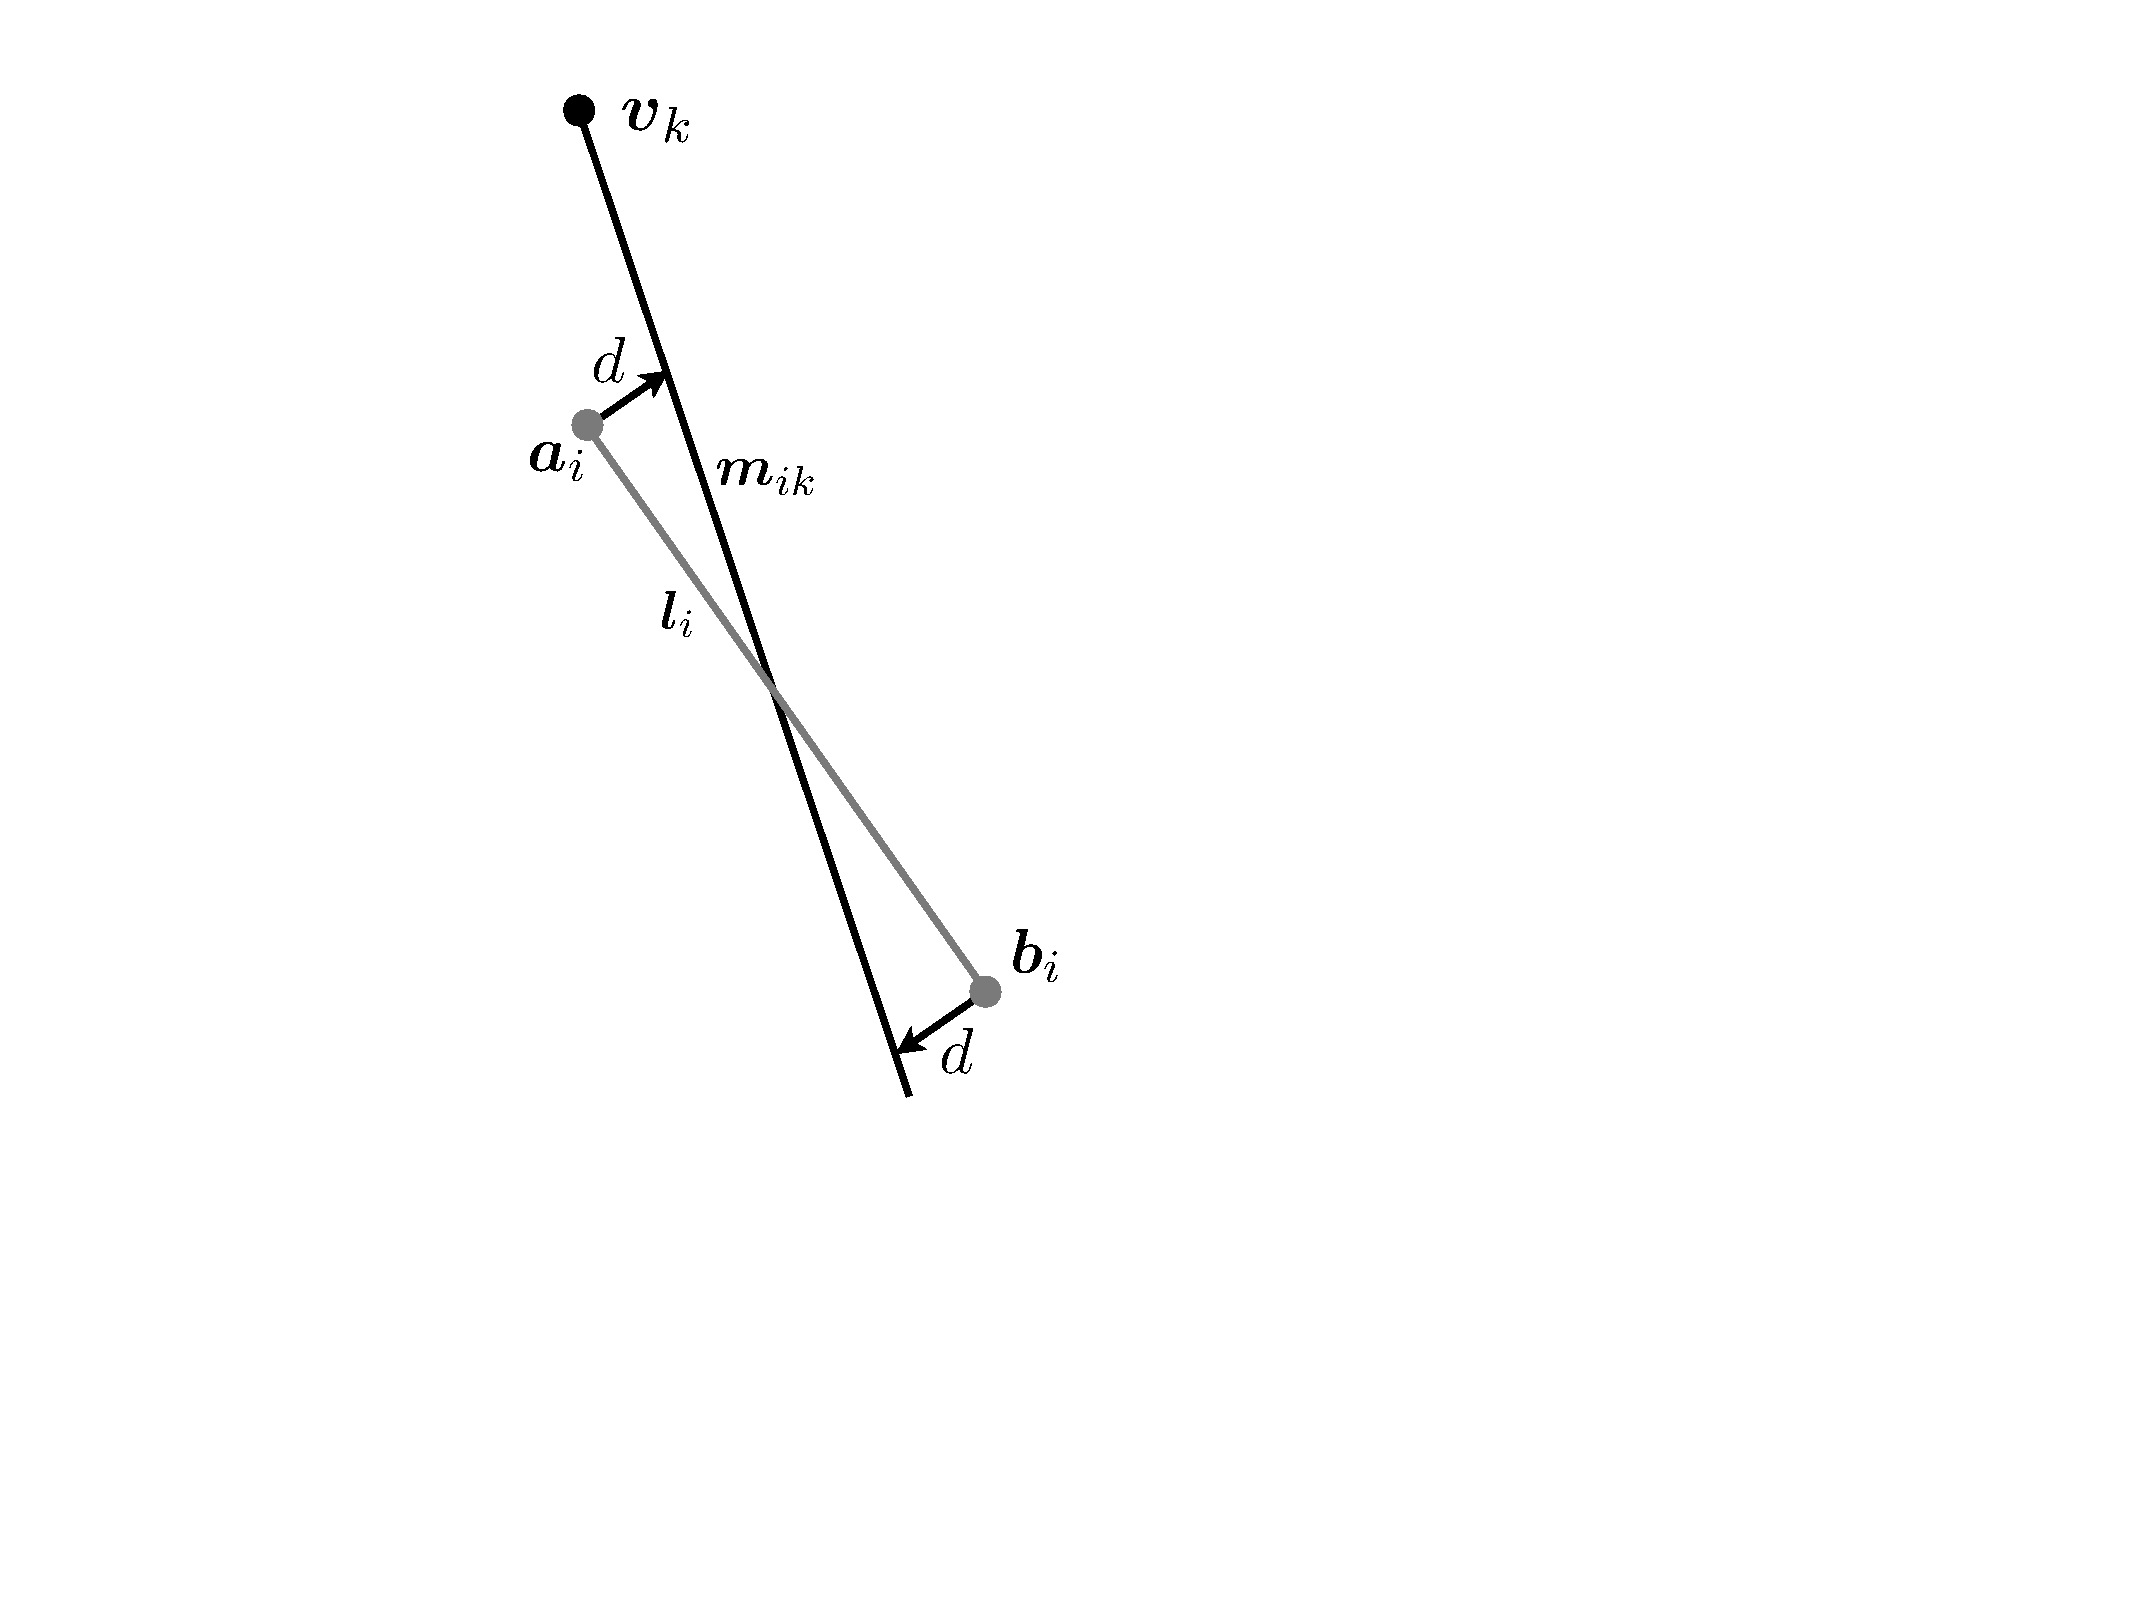
\includegraphics[width=0.4\textwidth]{reproj-dist}
  }  
  \caption{\changedsinceviva{Illustration of our error model and various geometric
    quantities involved in the derivations in the main text.}}
  \label{fig:line-model}
\end{figure}

We assume the graphical model shown in \figref{R-graphical}. The
generative process operates as follows. First we sample a scene
orientation $\SceneR$ and the rotation component of the camera pose,
$\CamR_j$ for each frame. (Camera translation plays no part when
reasoning about vanishing points.) Next we sample a discrete variable
$\Indicator_i$ from a categorical distribution with mixing parameters
$\Mixing$. The variable $\Indicator_i$ is a binary vector of length 4
indicating which vanishing point each line segment is associated
with. Exactly one element is set to 1, the other three are 0. The
first three elements correspond to the three vanishing points, the
fourth to a spurious observation not associated
with any of the three Manhattan directions. We denote the (binary)
value of the $k$\th element $\Indicator_{ik}$, but we will also write
$\Indicator_i=k$ as shorthand for the event that $\Indicator_i$ is the
binary vector with the $k$\th element set to 1. For clarity we write
$\Indicator_i=\Spurious$ in place of $\Indicator_i=4$. If
$\Indicator_i=\Spurious$ then the line segment $\TrueSeg_i$ is
sampled uniformly from the image. Otherwise, $\TrueSeg_i$ is
associated with the vanishing point $\vpt_{\Indicator_i}$ and is
sampled as follows.

The vanishing point corresponding to $\Indicator_i$ is
\begin{equation}
  \vpt_{\Indicator_i} = \CamR_j \SceneR \ebasis_{\Indicator_i} ~.
\end{equation}
We sample a ray through $\vpt$, then sample a line segment $\TrueSeg =
(\TrueStartPt,\TrueEndPt)$ along the ray. We add isotropic Gaussian
noise to arrive at the measured line segment
$\LineSeg=(\StartPt,\EndPt)$:
\begin{eqnarray}
  \StartPt &\sim& \NormalDistr(\TrueStartPt, \Sigma) \\
  \EndPt &\sim& \NormalDistr(\TrueEndPt, \Sigma) ~.
\end{eqnarray}
This process is illustrated by the graphical model in \figref{R-graphical}.

The likelihood for line segments is
\begin{equation}
  P(\LineSeg_i ~|~ \Indicator_i,\SceneR) =
  \NormalDistr(\dist(\LineSeg_i,\vpt_{\Indicator_i}); 0, \sigma)
\end{equation}
where $\dist(\LineSeg,\vpt)$ is the reprojection error illustrated in
\figref{line-model}. $\dist$ is computed as follows. First,
draw a line between the vanishing point $\vpt$ and the mid--point of
the line segment $\LineSeg$,
\begin{equation}
  \ReprojLine_{ik} =
  \vpt_k \cross \frac{\StartPt_i+\EndPt_i}{2}
\end{equation}
Now, $\dist$ is the distance between the line $\ReprojLine$ and either
of the two end points of $\LineSeg$ (the two quantities are equal, as
evident by inspecting \figref{line-model}). So
\begin{eqnarray}
  \dist(\LineSeg_i,\vpt_k) &=& 
  \frac
      {\StartPt_i \cdot \ReprojLine_{ik}}
      {(\StartPt_{i}\cdot\ez) \eta_{ik}}\\
      \eta_{ik} &=&
      \sqrt{(\ReprojLine_{ik} \cdot \ex)^2 +
        (\ReprojLine_{ik} \cdot \ey)^2}
      ~.
\end{eqnarray}

\section{Estimating the Manhattan Coordinate Frame}

We now turn to the inference algorithm that we use to find the
maximum--likelihood estimate of $\SceneR$ under the probabilistic
assumptions described in the previous section. We begin by running the
Canny edge detector \cite{Canny1986}, followed by an edge linking
algorithm \cite{Zhang02} to identify a set of straight line segments
$\LineSeg_j = \{\Pixel : \LineSeg_j\cdot\Pixel = 0\}$.

Under the model presented in the previous section, the
likelihood of $\SceneR$ is
\begin{equation}
  P(\LineSegs ~|~ \SceneR,\{\CamR_i\}) =
  \int P(\LineSegs,\Indicators ~|~ \SceneR,\{\CamR_i\})
  ~\intd\Indicators ~.
\end{equation}
For brevity we will omit the camera poses $\{\CamR_i\}$ in the
remainder of this section; it may be assumed that all probabilities
to follow are conditioned on $\{\CamR_i\}$.

The indicators $\Indicators$ are latent variables over which we need
to marginalise in order to perform inference on $\SceneR$. Integrating
explicitly is intractable so we turn to the
expectation--maximisation (EM) algorithm, which alternately refines
estimates of the posterior on $\Indicators$ (the ``E--step'') and
$\SceneR$ (the ``M--step'').

Due to the iterative nature of the EM algorithm we adopt superscript
notation for the scene rotation and indicators to make clear the
dependence between successive time steps. $\SceneR^t$ is the estimate
of the scene rotation at time $t$ and $\PosteriorEst^t$ is the
estimate for the posterior on $\Indicators$ at time $t$. Note that the
former is an estimate of a variable but the latter is an estimate of a
distribution. For notational convenience we will treat $\PosteriorEst$
as a continuous function, though of course in practice we really just
store sufficient statistics for $\PosteriorEst$. Also note that we
never actually store or estimate the values of the indicators
$\Indicators$, so we have no need for superscripts on this
variable. Although $\Indicators$ does appear in the derivations to
follow, in every equation we are either marginalising it out, or
defining a function over it.

\subsection{Complete Data Likelihood}

In sections to follow we will need to deal with the complete data
likelihood,
\begin{equation}
  P(\LineSegs,\Indicators ~|~ \SceneR) =
  \prod_i P(\LineSeg_i,\Indicator_i ~|~ \SceneR)
\end{equation}

The likelihood terms $P(\LineSeg_i,\Indicator_i ~|~ \SceneR)$ depend
on $\Indicator_i$ in a complicated way, since $\LineSeg_i$ is
drawn from a different distribution depending on $\Indicator_i$:
\begin{eqnarray}
  P(\LineSeg_i,\Indicator_i ~|~ \SceneR) &=&
  P(\Indicator_i ~|~ \SceneR)~
  P(\LineSeg_i, ~|~ \Indicator_i, \SceneR)\\
  &=&
  \begin{cases}
    \Mixing_1 
    \NormalDistr\bigr(\dist(\LineSeg_i, \CamR_i\SceneR\ex\bigl); 0,\sigma),
    & \mbox{if } \Indicator_i = 1 \\
    \Mixing_2
    \NormalDistr\bigr(\dist(\LineSeg_i, \CamR_i\SceneR\ey\bigl); 0,\sigma),
    & \mbox{if } \Indicator_i = 2 \\
    \Mixing_3
    \NormalDistr\bigr(\dist(\LineSeg_i, \CamR_i\SceneR\ez\bigl); 0,\sigma),
    & \mbox{if } \Indicator_i = 3 \\
    \Mixing_{\Spurious}
    \frac{1}{Z_\Spurious},
    & \mbox{if } \Indicator_i = \Spurious ~.
  \end{cases}
\end{eqnarray}
Due to our definition of $\Indicator_i$ as a binary vector we can
express this likelihood in the following analytic form,
\begin{equation}
  \label{eq:complete-likelihood}
  P(\LineSeg_i,\Indicator_i ~|~ \SceneR) =
  \prod_{k=1}^4 \Bigl( 
  P(\LineSeg_i ~|~ \Indicator_i=k,\SceneR)
  P(\Indicator_i=k ~|~ \SceneR)
  \Bigr)^{\Indicator_{ik}} ~.
\end{equation}

\subsection{The E--step}

During this phase we compute sufficient statistics for the posterior on
the indicators given a fixed estimate of $\SceneR$. This posterior
is
\begin{eqnarray}
  \PosteriorEst^t(\Indicators) &=&
  P(\Indicators ~|~ \LineSegs,\SceneR^t) \\
  \label{eq:posterior-est}
  &=&
  \frac{
    \prod_i P(\LineSeg_i,\Indicator_i ~|~\SceneR^t)
  }{
    \int \prod_i P(\LineSeg_i,\Indicator_i ~|~ \SceneR^t)
    ~\intd\Indicators
  }
\end{eqnarray}
Consider the term on the top line,
\begin{equation}
  P(\LineSeg_i,\Indicator_i ~|~\SceneR^t)
  =
  P(\LineSeg_i ~|~ \Indicator_i,\SceneR^t)
  P(\Indicator_i ~|~ \SceneR^t) ~.
\end{equation}
As a function of $\Indicator_i$ this is simply a categorical
distribution: $\Indicator_i$ can take on 3 possible values, and we can
compute each explicitly since $\SceneR^t$ and $\LineSeg_i$ are
fixed. Now since equation \eqnref{posterior-est} is a
normalised concatenation of categorical distributions, it is
itself a categorical distribution, meaning that the sufficient
statistics for $\PosteriorEst^t$ are the
expectations
\begin{eqnarray}
  \Expected_{\PosteriorEst^t}\bigl[ \Indicator_{ik} \bigr]
  &=& 
  \int \Indicator_{ik} \PosteriorEst^t(\Indicators) ~\intd\Indicators \\
  &=& 
  \sum_{\Indicator_{ik}\in\{0,1\}}
  \Indicator_{ik} P(\Indicator_{ik} ~|~ \LineSeg_i, \SceneR^t)\\
  &=&
  P(\Indicator_i=k ~|~ \LineSeg_i, \SceneR^t)\\
  &=&
  \label{eq:expected-zik}
  \frac
      {P( \LineSeg_i, \Indicator_i=k ~|~ \SceneR^t)}
      {\sum_{j=0}^4 P(\LineSeg_i, \Indicator_i=j ~|~ \SceneR^t)}
\end{eqnarray}
where in the third line we have expanded the sum over the two possible
values for $\Indicator_{ik}$ and cancelled the one in which
$\Indicator_{ik}$ is 0. Substituting the specific forms for the the
complete data likelihood \eqnref{complete-likelihood},
\begin{eqnarray}
  \Expected_{\PosteriorEst^t}\bigl[ \Indicator_{ik} \bigr] 
  &=&
  \frac{
    \prod_{k=1}^4\limits \Bigl( 
    P(\LineSeg_i ~|~ \Indicator_i=k,\SceneR^t)
    P(\Indicator_i=k ~|~ \SceneR^t)
    \Bigr)^{\Indicator_{ik}}
  }{
    \sum_{\Indicator_i=1}^4\limits
    \prod_{k=1}^4\limits \Bigl( 
    P(\LineSeg_i ~|~ \Indicator_i=k,\SceneR^t)
    P(\Indicator_i=k ~|~ \SceneR^t)
    \Bigr)^{\Indicator_{ik}}
  }\\
  \label{eq:big-expectation}
  &=&
  \frac{
    \Bigl(
    \Mixing_{\Spurious}
    P(\LineSeg_i ~|~ \Indicator_i=\Spurious,\SceneR^t)
    \Bigr)^{\Indicator_{ik}}
    \prod_{k=1}^3\limits \Bigl(
    \Mixing_k
    P(\LineSeg_i ~|~ \Indicator_i=k,\SceneR^t)
    \Bigr)^{\Indicator_{ik}}
  }{
    \sum_{\Indicator_i=1}^4\limits \Biggl[
      \Bigl(
      \Mixing_{\Spurious}
      P(\LineSeg_i ~|~ \Indicator_i=\Spurious,\SceneR^t)
      \Bigr)^{\Indicator_{ik}}
      \prod_{k=1}^3\limits \Bigl( 
      \Mixing_k
      P(\LineSeg_i ~|~ \Indicator_i=k,\SceneR^t)
      \Bigr)^{\Indicator_{ik}}
      \Biggr]
  }~.
\end{eqnarray}
We now define
\begin{eqnarray}
  \SpurJoint_i &=& 
  \Mixing_{\Spurious}
  P(\LineSeg_i ~|~ \Indicator_i=\Spurious,\SceneR^t) \\
  \SpurIndicator_i &=&
  \begin{cases}
    1, & \mbox{if } \Indicator_i = \Spurious \\
    0, & \mbox{otherwise}
  \end{cases}
\end{eqnarray}
and substituting into \eqnref{big-expectation} we have
\begin{eqnarray}
  \Expected_{\PosteriorEst^t}\bigl[ \Indicator_{ik} \bigr]
  &=&
  \frac{
    \SpurJoint_i^{\SpurIndicator_i}
    \Bigl(
    \Mixing_{\Indicator_i}
    \NormalDistr(\dist(\LineSeg,\CamR_i\SceneR^t\ebasis_k); 0, \sigma)
    \Bigr)^{1-\SpurIndicator_i}
  }{
    \sum_{\Indicator_i=1}^4\limits
    \SpurJoint_i^{\SpurIndicator_i}
    \Bigl(
    \Mixing_{\Indicator_i}
    \NormalDistr(\dist(\LineSeg,\CamR_i\SceneR^t\ebasis_{\Indicator_i}); 0, \sigma)
    \Bigr)^{1-\SpurIndicator_i}
  }\\
  &=&
  \frac{
    \SpurJoint_i^{\SpurIndicator_i}
    \Bigl(
    \Mixing_{\Indicator_i}
    \NormalDistr(\dist(\LineSeg,\CamR_i\SceneR^t\ebasis_k); 0, \sigma)
    \Bigr)^{1-\SpurIndicator_i}
  }{
    \SpurJoint_i +
    \sum_{\Indicator_i=1}^3\limits
    \Bigl(
    \Mixing_{\Indicator_i}
    \NormalDistr(\dist(\LineSeg,\CamR_i\SceneR^t\ebasis_{\Indicator_i}); 0, \sigma)
    \Bigr)
  }~.
  \label{eq:final-estep}
\end{eqnarray}
The E--step therefore consists of computing the expectations for
each indicator according to \eqnref{final-estep}, which are sufficient
statistics for the posterior on $\Indicators$. The expression
above can be evaluated for each indicator in constant time, leading to
a complexity for the E--step linear in the number of observed line
segments.

\subsection{M--step}
\label{sect:mstep}

During this phase we compute $\SceneR^{t+1}$ as the maximiser of the
expectation of the complete data log--likelihood under the (fixed)
distribution $\PosteriorEst^t$. The logarithm of the complete data
log--likelihood \eqnref{complete-likelihood} is
\begin{eqnarray}
  \log P(\LineSegs,\Indicators ~|~ \SceneR) 
  &=&
  \sum_i \sum_{k=1}^4 \Indicator_{ik} \Bigl(
  \log P(\LineSeg_i ~|~ \Indicator_i=k, \SceneR)
  + \log P(\Indicator_i=k ~|~ \SceneR)
  \Bigr)\\
  &=&
  \sum_i \sum_{k=1}^4 \Indicator_{ik} 
  \Bigl(
  \log \NormalDistr(\dist(\LineSeg_i, \CamR_i\SceneR\ebasis_k);0,\sigma)
  + \log \Mixing_k
  \Bigr)\\
  &=&
  \sum_i \sum_{k=1}^4 \Indicator_{ik} 
  \Bigl(
  \frac{-\dist(\LineSeg_i, \CamR_i\SceneR\ebasis_k)^2}{2\sigma^2}
  + \log \Mixing_k
  \Bigr) + c
\end{eqnarray}
where $c$ is a constant arising from the logarithm of the normal
distribution, which we now drop since it plays no part in the
maximisation to follow. The expectation of the above with respect to
the distribution $\PosteriorEst^t$ is
\begin{eqnarray}
  \Expected_{\PosteriorEst^t}\Bigl[
    \log P(\LineSegs,\Indicators ~|~ \SceneR) 
    \Bigr]
  &=&
  \sum_i \sum_{k=1}^4
  \Expected_{\PosteriorEst^t} \bigl[ \Indicator_{ik} \bigr]
  \Bigl(
  \frac{-\dist(\LineSeg_i, \CamR_i\SceneR\ebasis_k)^2}{2\sigma^2}
  + \log \Mixing_k
  \Bigr)\\
  &=&
  \label{eq:expected-lik}
  \sum_i \sum_{k=1}^4
  \Resp_{ik}^t
  \Bigl(
  \frac{-\dist(\LineSeg_i, \CamR_i\SceneR\ebasis_k)^2}{2\sigma^2}
  + \log \Mixing_k
  \Bigr)
\end{eqnarray}
where in the last line we have defined and substituted
\begin{equation}
  \Resp_{ik}^t = 
  \Expected_{\PosteriorEst^t} \bigl[ \Indicator_{ik} \bigr] ~.
\end{equation}

The maximisation we wish to perform is
\begin{equation}
  \label{eq:R-argmax}
  \SceneR^{t+1} = \argmax_{\SceneR}\limits
  \Expected_{\PosteriorEst^t}\Bigl[
    \log P(\LineSegs,\Indicators ~|~ \SceneR) 
    \Bigr] ~.
\end{equation}
It is worth examining the expression being maximised and noting which
variables it is and is not a function of. During each M--step, the
distribution $\PosteriorEst^t$, as represented by the sufficient
statistics computed in the E--step, is held fixed. The expectation is
over all possible values of the indicators $\Indicators$, each
weighted according to $\PosteriorEst^t$, which was computed from the
previous estimate $\SceneR^t$ but does not depend on the quantity
$\SceneR$ being maximised in this step. Hence the expression being
maximised in \eqnref{R-argmax} is a function of $\SceneR$ alone. Substituting
\eqnref{expected-lik},
\begin{eqnarray}
  \SceneR^{t+1} &=& \argmax_{\SceneR}\limits \ErrorFunc(\SceneR) \\
  \ErrorFunc(\SceneR) 
  &=&
  \label{eq:R-error}
  \sum_i \sum_{k=1}^4
  \Resp_{ik}^t
  \Bigl(
  \frac{-\dist(\LineSeg_i, \CamR_i\SceneR\ebasis_k)^2}{2\sigma^2}
  + \log \Mixing_k
  \Bigr)~.
\end{eqnarray}
Importantly, note that $\Resp_{ik}^t$ is a constant with respect to
$\SceneR$ in the above. We perform the maximisation
\eqnref{R-argmax} by gradient descent. Differentiating
\eqnref{R-error} with respect to $\SceneR$,
\begin{eqnarray}
  \Deriv{\ErrorFunc}{\SceneR}
  &=&
  \sum_i \sum_{k=1}^4
  \Resp_{ik}^t
  \Bigl(
  \frac{-\dist_{ik}}{\sigma^2}
  \Deriv{\dist_{ik}}{\SceneR} 
  \Bigr)\\
  \Deriv{\dist_{ik}}{\SceneR} &=&
  \frac{1}{\StartPt_i \cdot \ez} 
  \Biggl(
  % THIS NEGATION is swapped from some of the equations in my
  % notebook because the cross product matrix term at the end is negative
  \frac
      {(\ReprojLine_{ik})_1\ex + (\ReprojLine_{ik})_2\ey}
      {{\eta_{ik}}^3}
      (\ReprojLine_{ik} \cdot \StartPt_i)
      -
      \frac{\StartPt_i}{\eta_{ik}}
      \Biggr)
      \Bigl[ \frac{\StartPt_i+\EndPt_i}{2} \Bigr]_{\cross}
      \Deriv{\vpt_k}{\SceneR}
\end{eqnarray} 
where
\begin{eqnarray}
  \dist_{ik} &=& \dist(\LineSeg_i, \CamR_i\SceneR\ebasis_k)\\
  \eta_{ik} &=&
  \sqrt{(\ReprojLine_{ik} \cdot \ex)^2 +
    (\ReprojLine_{ik} \cdot \ey)^2}
\end{eqnarray}
and
\begin{equation}
  \bigl[ \vect{x} \bigr]_{\!\cross} = 
  \begin{bmatrix}
    0 & -x_3 & x_2 \\
    x_3 & 0 & -x_1 \\
    -x_2 & x_1 & 0
  \end{bmatrix}
\end{equation}
is the matrix form for the cross product.

For the purpose of optimisation we write $\SceneR$ as the product of a
fixed part $R_0$ and a variable part $R_{\delta}$, the latter of which
is represented in the Lie algebra for the special orthogonal group
$SO(3)$, so
\begin{eqnarray}
  \SceneR &=& R_0 R_{\delta} \\
  R_{\delta} &=& \exp\Bigl(\sum \LieM_i \Gen_i\Bigr)
\end{eqnarray}
where the $\Gen_i$ are the generator matrices for $SO(3)$ and the
$\LieM_i$ provide a minimal representation for the 3D rotation matrix
group. The advantage of using this representation is that after each
gradient step we are guaranteed that $\SceneR$ remains a pure
rotation, unlike under other representations such as optimising the
elements of the $3 \times 3$ rotation matrix directly. Differentiating
$\vpt$ with respect to $\LieMs$ yields
\begin{equation}
  \Deriv{\vpt_k}{\LieMs} = \CamR_i \Deriv{\SceneR}{\LieMs} \ebasis_k ~.
\end{equation}
The division of $\SceneR$ into fixed and variable parts allows us to
evaluate the gradient at $\LieMs=0$ without loss of generality. In
this case,
\begin{equation}
  \Deriv{\vpt_k}{\LieMs} \EvalAt{\LieMs=0} =
  \begin{bmatrix}
    \CamR_i R_0 \Gen_1 \ebasis_k &
    \CamR_i R_0 \Gen_2 \ebasis_k &
    \CamR_i R_0 \Gen_3 \ebasis_k
  \end{bmatrix}~.
\end{equation}

This completes the derivation of the gradient of the error function
$\ErrorFunc$ with respect to the parametrisation $\LieMs$. We proceed as
normal with gradient steps of the form
\begin{equation}
  \LieMs^{t+1} = \LieMs^t - \gamma \Deriv{\ErrorFunc}{\LieMs} ~.
\end{equation}

Due to the low dimensionality of the search space and relatively low
curvature of the error function we found that a simple instantiation
of the gradient descent algorithm converged quickly and robustly. Our
algorithm initialises the step size $\gamma$ to a fixed constant
$\gamma_0$ at the beginning of each M--step, then divides $\gamma$ by
2 each time that an update leads to an increase in the error
function. Convergence is detected when $\gamma<\epsilon_1$ and the
value of the error function decreases by less than $\epsilon_2$ in any
one update.

\subsection{Initialisation}

\changedsinceviva{
We initialise our EM algorithm using the clustering approach described
by Koseck\`{a} and Zhang \cite{Zhang02}. This process begins by
clustering observed line segments according to their orientation in
the image plane, the basis for this being that Manhattan environments
often contain Manhattan--oriented lines that are close to one another
(relative to the distance to the vanishing point), and hence appear
almost parallel. We run K--means clustering on all line segments in
each image separately (with $K=5$) then we estimate a least--squares
vanishing point for each cluster that has at least 5 associated line
segments. Finally we project vanishing points from all frames onto the
plane at infinity and pick three that are close to mutually orthogonal
(by enumerating all combinations). We initialise the EM algorithm with
an (orthonormalized) rotation matrix containing the chosen vanishing
points as columns.
}

\subsection{Summary}
To obtain $\SceneR$ we iterate between updating $\PosteriorEst$ (the
E--step) and optimising $\SceneR$ (the M--step). Each M step consists
of a gradient descent in the Lie group $SO(3)$. In practice we find
that our system converged in around 25 iterations of the EM algorithm,
and that approximately 10 steps were required for each gradient
descent.

\section{Results}

We evaluated our approach using a dataset of 18 video sequences of 8
unique places, which we collected in indoor environments such as homes
and office spaces. We ran \changedsinceviva{an} off--the--shelf bundle
adjuster on each sequence to yield calibrated views, then transformed
each sequence by a random 3D rotation to eliminate any bias in the
initial conditions for our optimisation that might have been
introduced by structure--from--motion. We manually provided the ground
truth scene orientation $\SceneR$ for each sequence. We sampled frames
at regular intervals of approximately one second, then divided all
sequences into successive 7--frame blocks. Each such block is a single
``evaluation instance'' in our dataset.

We compared four approaches including our own. First, the
surface--normal--based approach of \cite{Furukawa09} described at the
beginning of this chapter, which we refer to by symbol ``NRM''. For
each evaluation instance, this algorithm received as input all
reconstructed 3D points that were visible in any of the 7 views in
that instance. We were generous to this approach here since the
reconstruction of some of these points may have relied upon data from
other frames. Second, we tested a system identical
to ours but in which the reconstruction error was replaced by the
algebraic error --- we refer to this system as ``ALG'' below. Finally, we
evaluated our own system using both a single input view (``SIN''), and
all 7 views (``MUL''). The former approach is hence similar to that of
Schindler and Dellaert \cite{Schindler2004}.

The metric we used to compare the estimated and ground truth
rotations was
\begin{equation}
  \| R_1^T R_2 - I \|_{\mathcal{F}} ~.
  \label{eq:rotation-metric}
\end{equation}
where $\|\cdot\|_{\mathcal{F}}$ denotes the Frobenius norm. We chose
this metric because it was shown by Huynh \cite{Huynh2009} to be
iso--equivalent to many 3D rotation metrics in common usage within
the computer vision literature, including quaternion norms and inner
products, and metrics based on Euler angles and the Lie algebra
$so(3)$.

\tableref{rot-performance} summarises the performance of each
algorithm. Unsurprisingly, the surface normal approach fails under the
sparse structure--from--motion point clouds --- it was proposed in the
context of dense reconstructions. Strikingly, the multiple--view
algebraic minimiser performs consistently worse than single--image
estimation. \changedsinceviva{Our investigations suggest that this is because the
algebraic error is an even poorer approximation to the reprojection
error in the multiple view context than in the single--view context,
since among many frames there is a high likelihood of observing a
vanishing point close to infinity. As a vanishing point moves towards
infinity, the algebraic error diverges from the reprojection error,
and the error terms for vanishing points near infinity to dominate the
objective function. This leads to poorly reconstructed vanishing
points since the optimisation focuses almost exclusively on these
very large error terms, ignoring the majority of the image evidence.
}

We ran a separate experiment to explore the relationship between the
number of frames used for estimation and the quality of the estimated
rotation; these results are shown in \figref{error-vs-nframes}. As the
number of frames used for estimation increases, the quality of the
estimator described in this chapter improves as expected. However, it
is interesting to note that the algebraic minimiser actually degrades
for more than 5 input frames. This supports our hypothesis above that
the algebraic error is an even poorer choice in the multiple--view
context than for single images.

Our third experiment explored the convergence properties of the
gradient descent component of our optimisation. Starting from an
initial rotation a specified distance from the ground truth, we
plotted the progress of our algorithm after each gradient step
(\figref{rotation-convergence}). In this experiment the indicators
$\Indicators$ were assumed known. Progress was measured both in terms
of the log--likelihood, which the optimiser itself has access to
(lower figure), and distance to ground truth, which the optimiser
obviously does not have access to (upper figure). This experiment
shows two things. First, that the basin of attraction is very wide ---
convergence is robust for distances up to $1.0$, which is a large
distance in the metric \eqnref{rotation-metric}. Second, that the
log-likelihood accurately tracks the ground truth error in practice,
since the runs that did not converge to the ground truth also
terminated at much lower log--likelihoods.

Finally, examples of the output from the four systems described above
are shown in Figures \ref{fig:vpt-example1}, \ref{fig:vpt-example2},
and \ref{fig:vpt-example3}.


%\figref{bathroom-vpts} shows the vanishing points identified in one of
%our sequences. Since each frame is informed by the entire sequence we
%are able to identify a globally consistent coordinate frame where
%single--image vanishing point detection fails. \figref{vpt-comparison}
%shows a side--by--side comparison with the single--image vanishing
%point detector of \cite{Zhang02}. Recently proposed improvements to
%the single--image approach \cite{Tardif09} may improve slightly on
%these, but we found that in cases where the single--image approach
%fails there is often simply not enough information available in
%individual frames to identify the appropriate coordinate frame, so any
%single--image approach will necessarily fail.

\begin{table}[tb]
  \centering
  \begin{tabular}{@{}p{2cm}p{3cm}p{3cm}p{3cm}p{3cm}@{}}
    \toprule
    Sequence & Error for NRM & Error for ALG & Error for SIN & Error
    for MUL \\
    \midrule
    \tt{Kitchen}  & 0.53   & 0.59   & 0.037  & \textbf{0.019} \\
    \tt{Foyer 1}   & 0.72   & 0.77   & 0.054  & \textbf{0.039} \\
    \tt{Foyer 2}  & 0.81   & 0.75   & 0.070  & \textbf{0.021} \\
    \tt{Bursary}  & 0.50   & 0.53   & 0.067  & \textbf{0.030} \\
    \tt{Ground}   & 0.90   & 0.68   & \textbf{0.55}   & 0.66 \\
    \tt{Atrium}   & 0.84   & 1.00   & 0.31  & \textbf{0.16} \\
    \tt{MCR}      & 0.56   & 0.56   & 0.06  & \textbf{0.04} \\
    \tt{Corridor} & 0.58   & 0.78   & \textbf{0.20}  & 0.21 \\
    \bottomrule
  \end{tabular}
  \vspace{0.2cm}
  \caption{Distance between estimated and ground truth rotation for
    four algorithms. Each cell shows the average error over all frames
    within a given sequence. From left to right the algorithms are
    the point--cloud procedure of \cite{Furukawa09} (NRM),
    Expectation--Maximisation using the algebraic error (ALG),
    Expectation--Maximisation using the geometric error applied to
    single (SIN) and multiple (MUL) images. All algorithms other than
    SIN were given 7 input frames in this experiment.}
  \label{table:rot-performance}
\end{table}

\begin{figure}[p]
  \centering
  \subfloat[Estimation error versus number of input frames.]{
    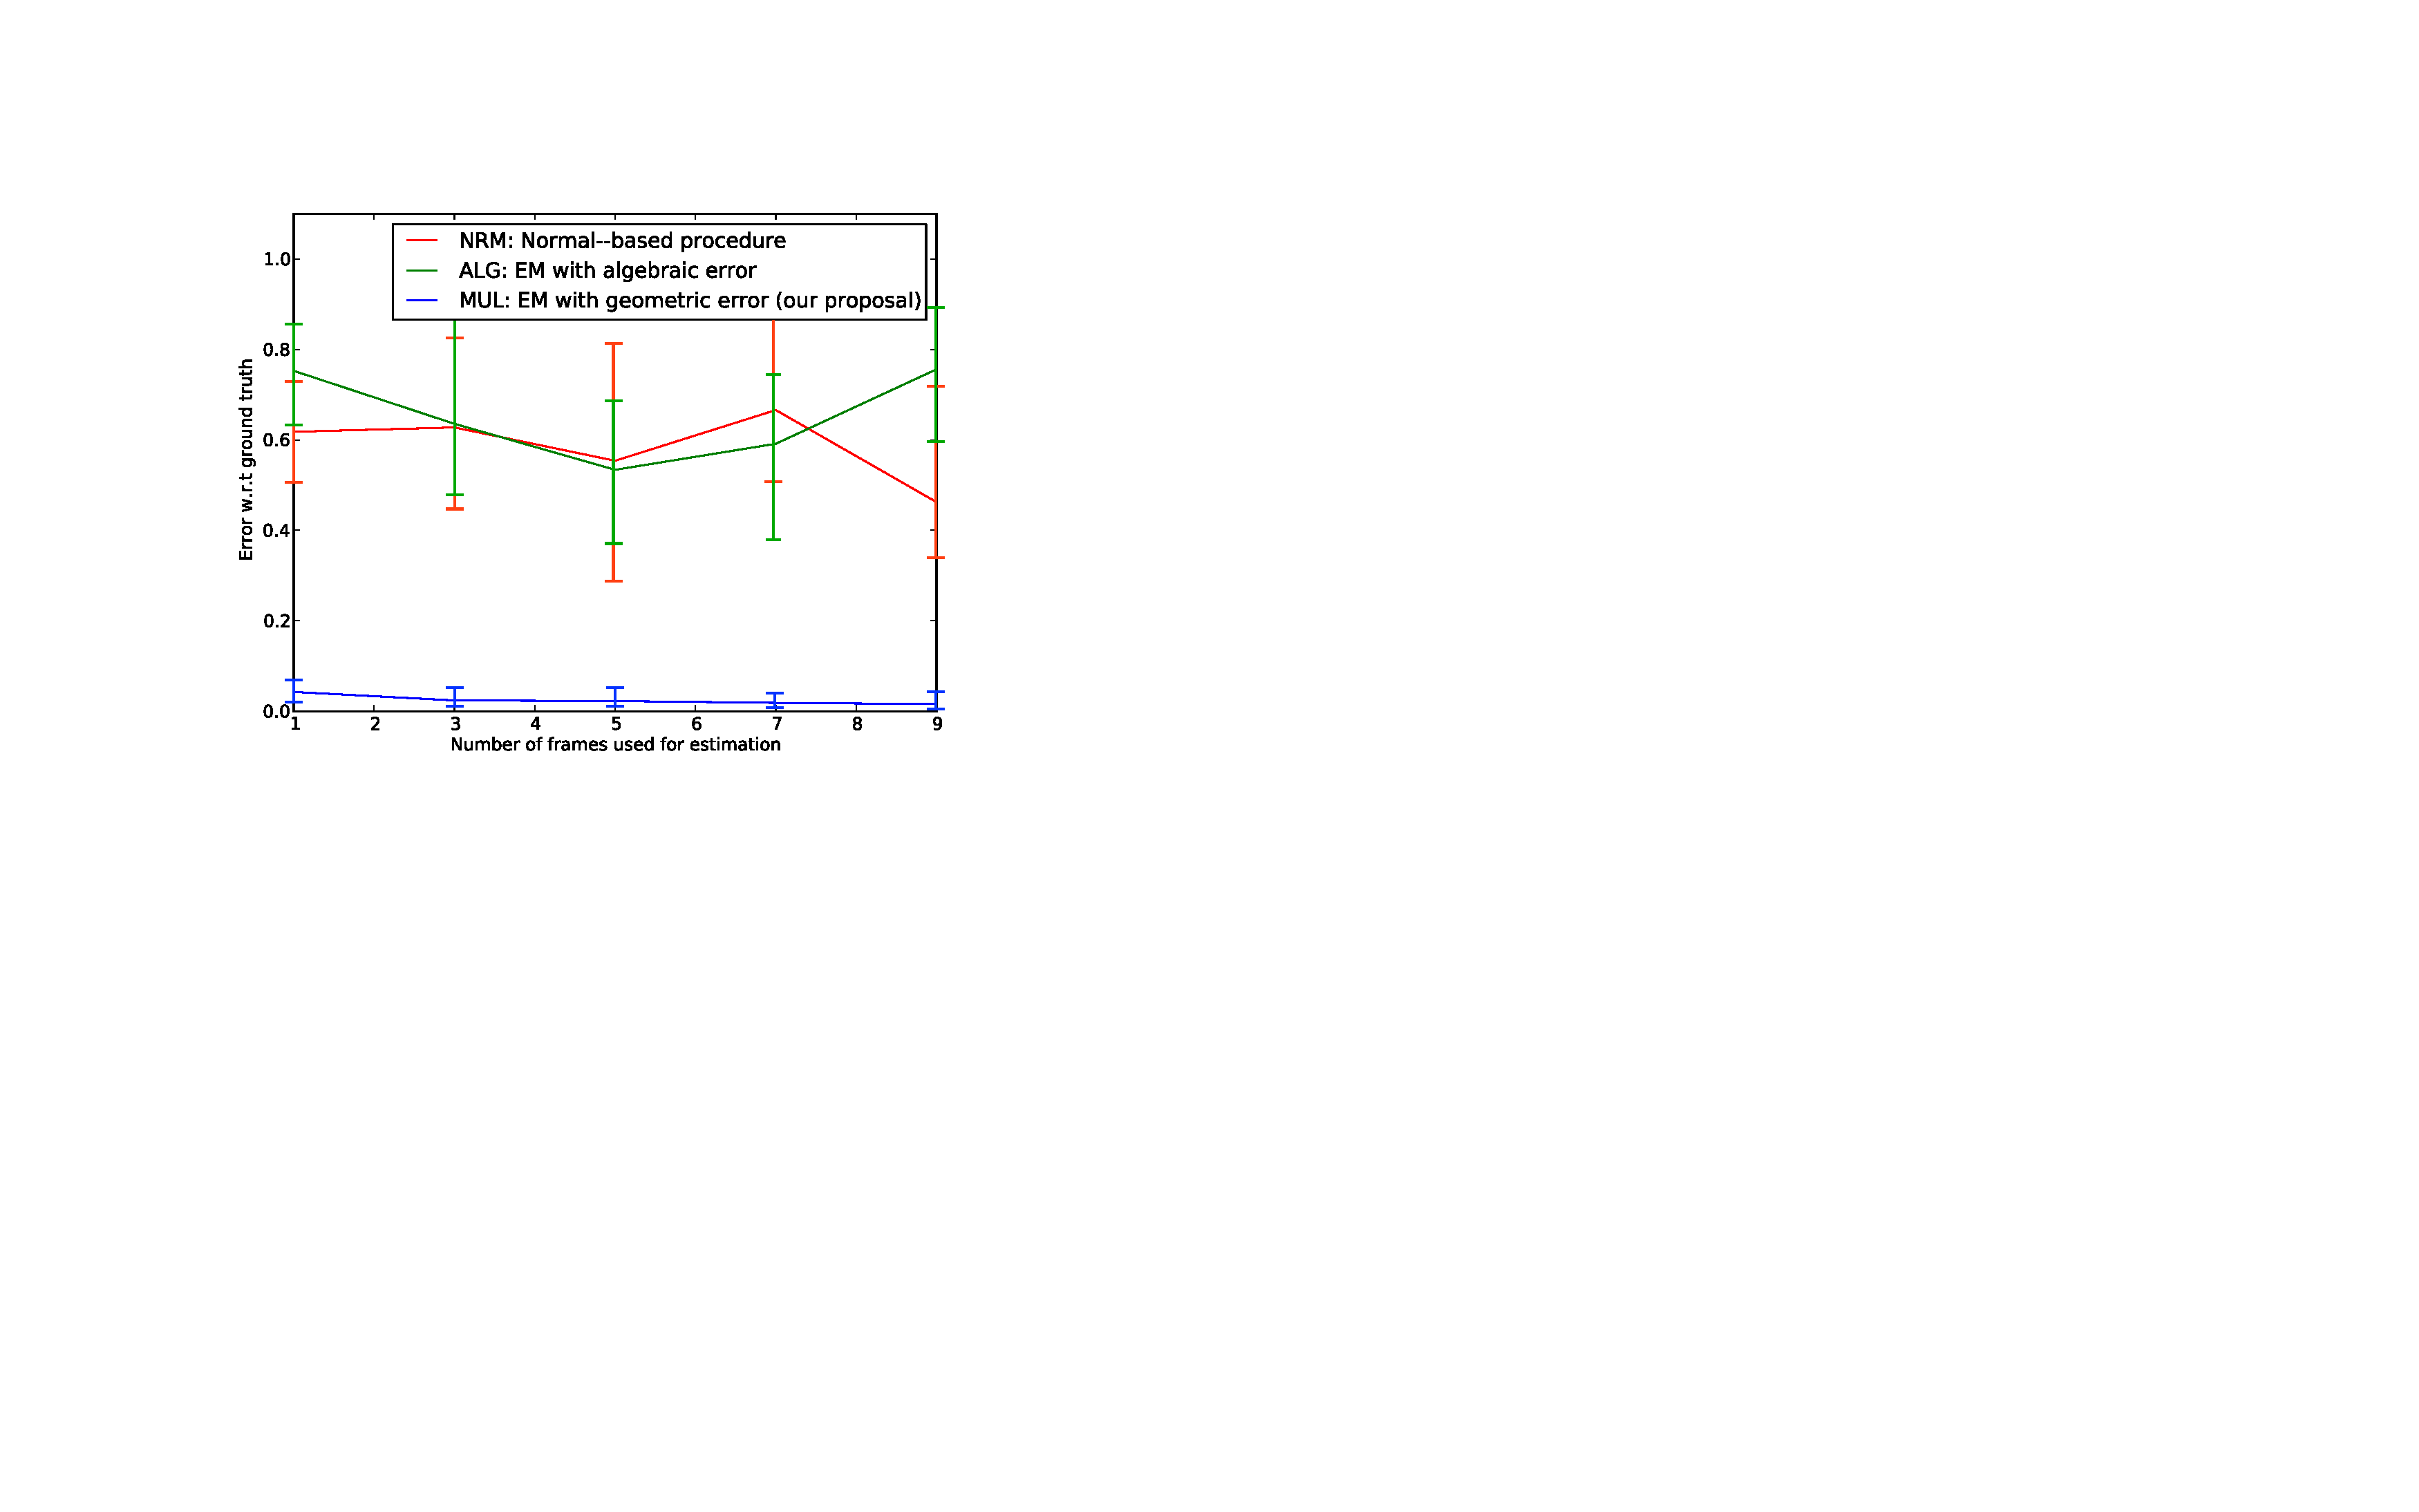
\includegraphics[width=0.65\textwidth]{plots/error_vs_nframes_with_errorbars}
  }
  \\
  \subfloat[A magnification of the third series above.]{
    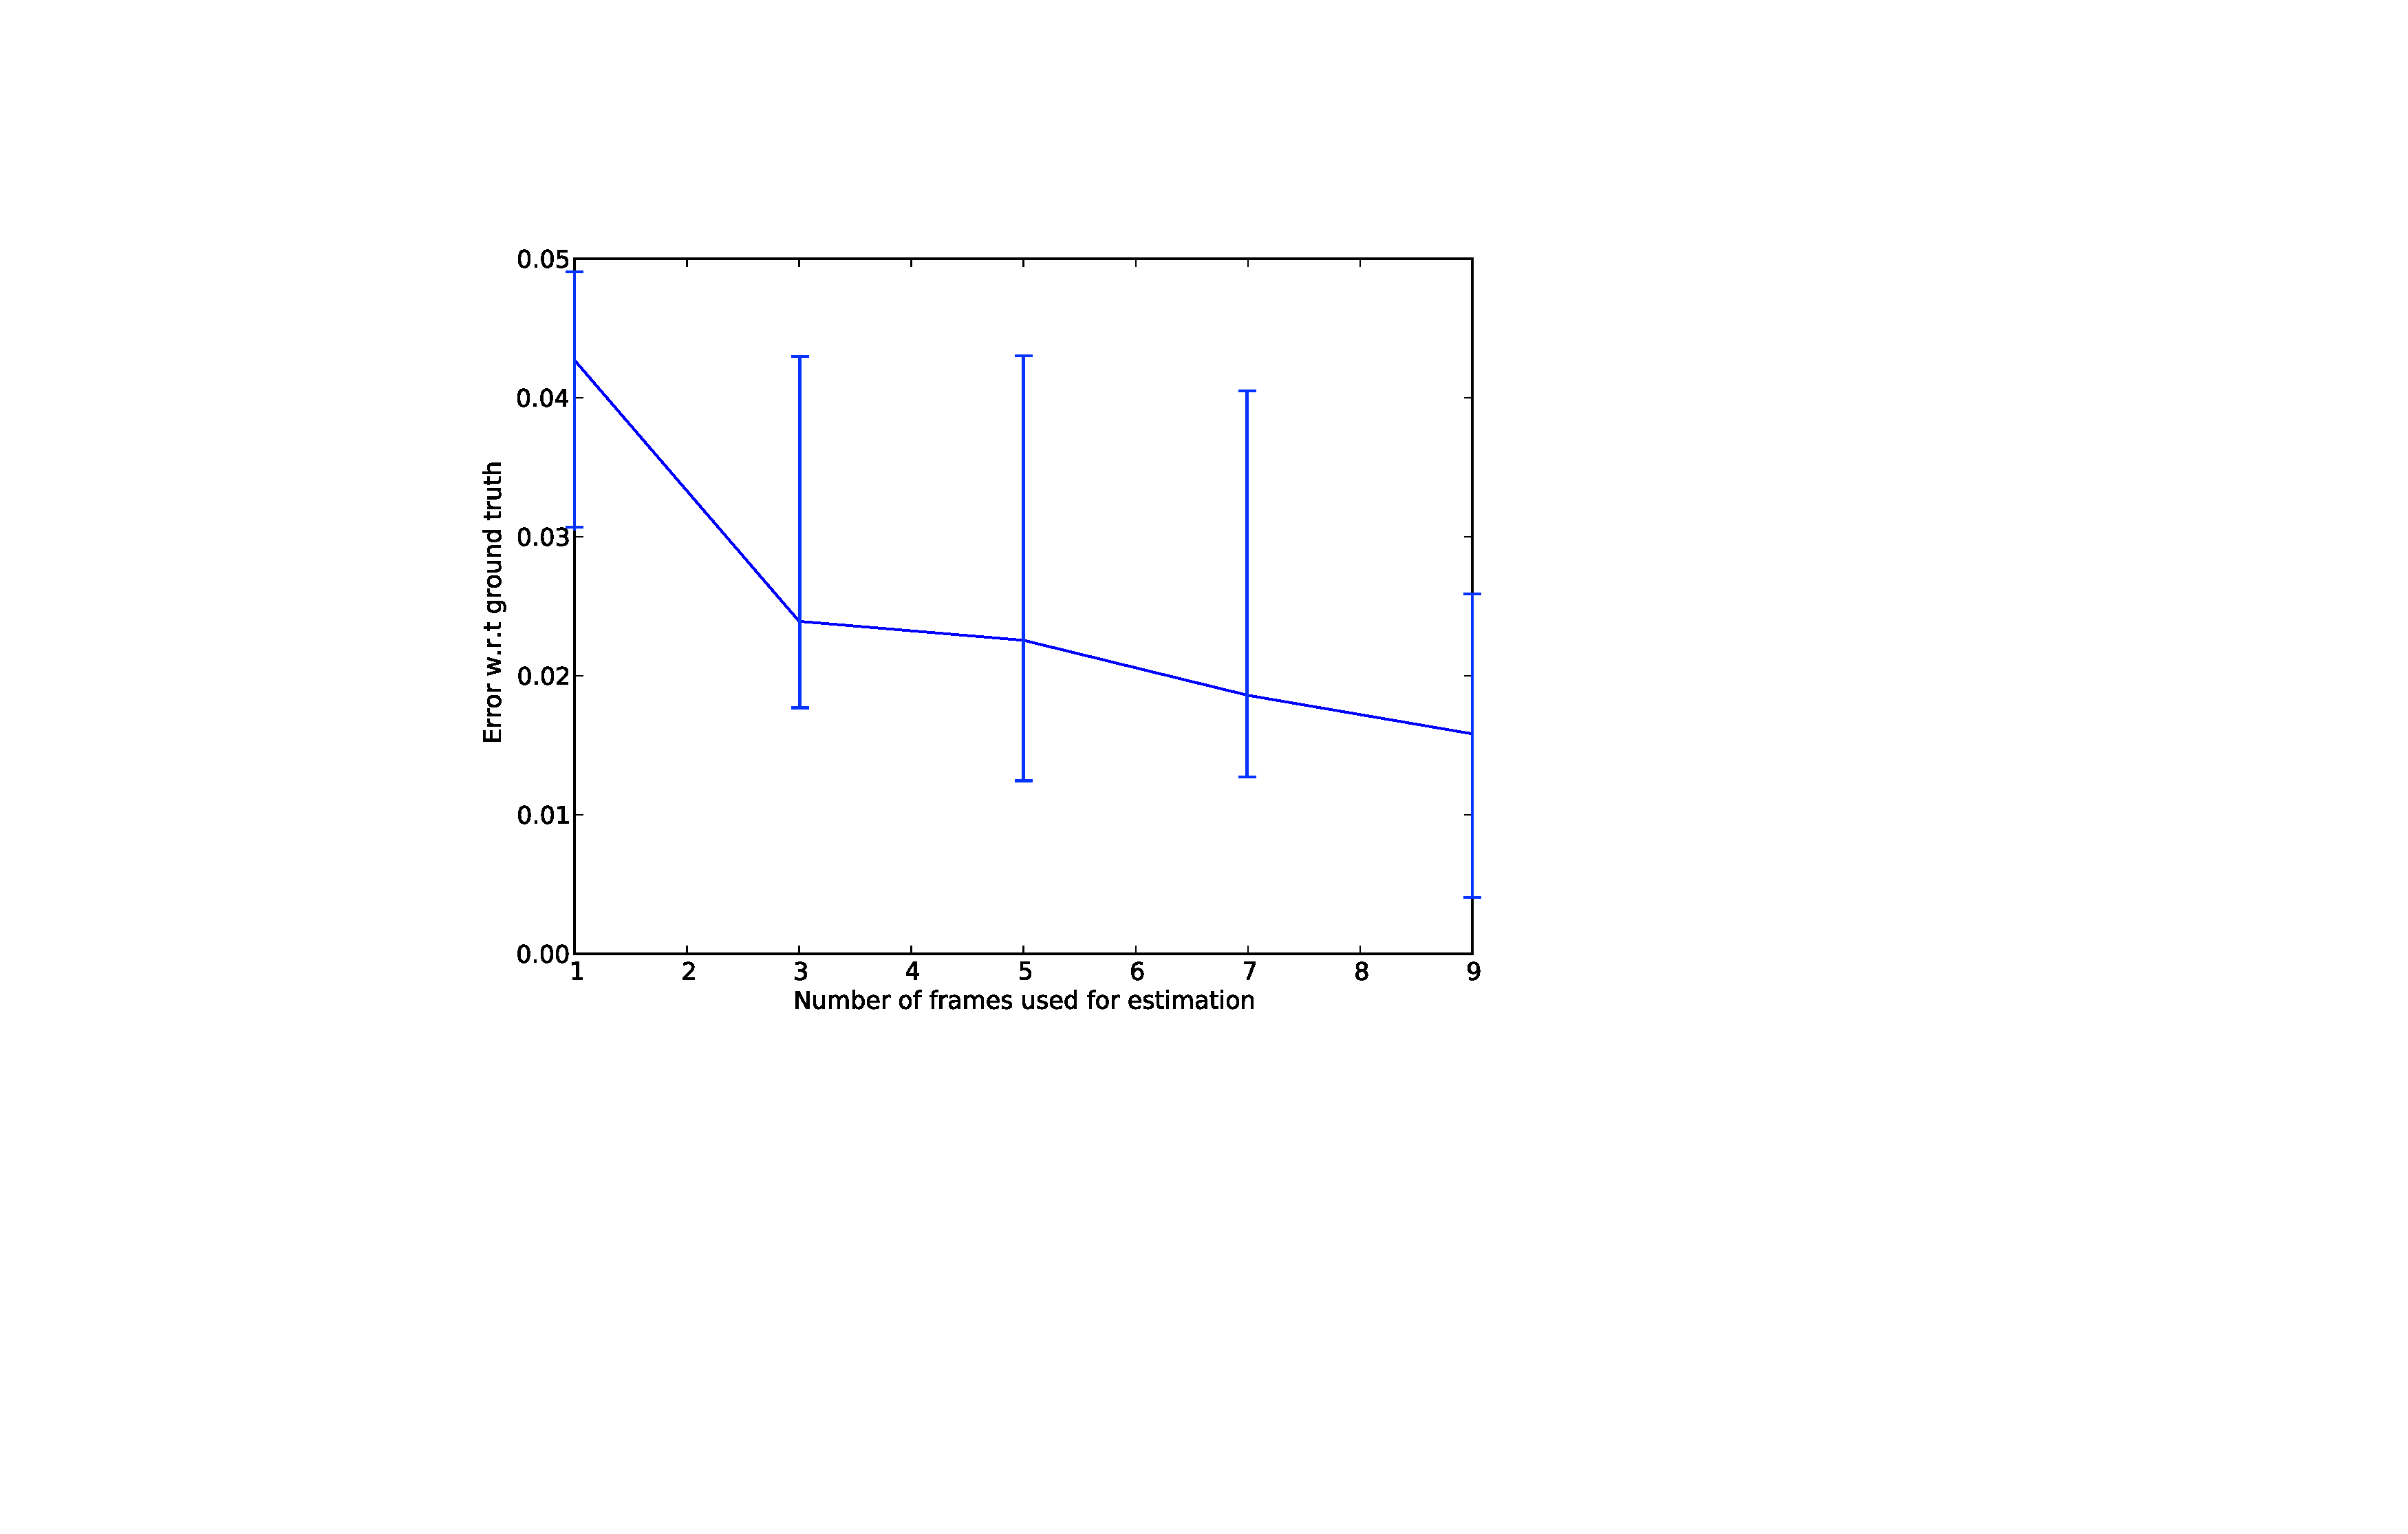
\includegraphics[width=0.65\textwidth]{plots/error_vs_nframes_oursonly_with_errorbars}
  }
  \caption{\changedsinceviva{Plots showing the performance of three algorithms as the
    number of input frames is increased. We compute each data point by
    executing the relevant algorithm on sets of $n$ consecutive frames
    drawn from our dataset, where $n$ is the value shown on the
    $x$--axis. The $y$--axis shows the average distance between the
    estimated and ground truth rotation, with error bars showing 90\%
    confidence intervals for the observed error distributions.}}
  \label{fig:error-vs-nframes}
\end{figure}


\begin{figure}[tb]
  \centering
  \subfloat[Convergence of error (with respect to ground truth)]{
    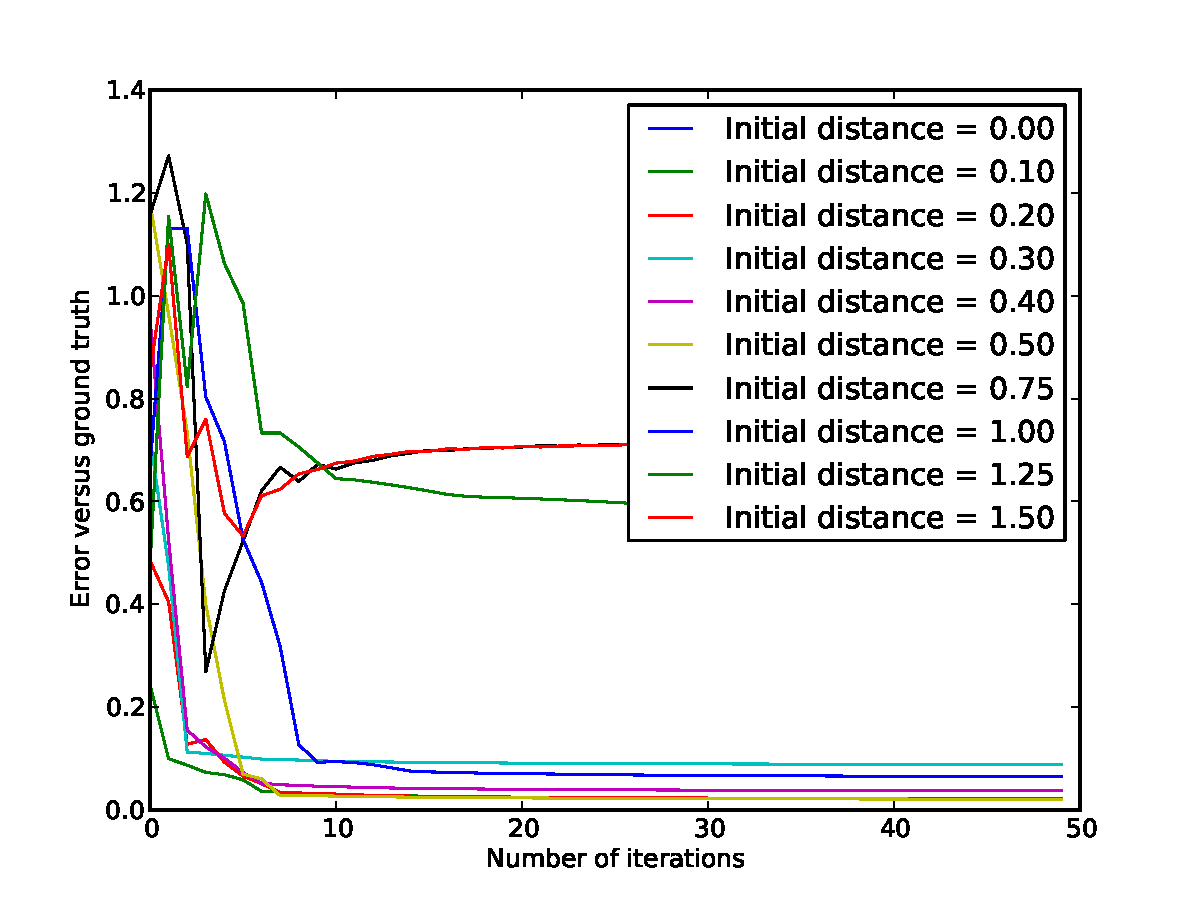
\includegraphics[width=0.65\textwidth]{plots/rotation_convergence_gterror}
  }
  \\
  \subfloat[Convergence of log--likelihood]{
    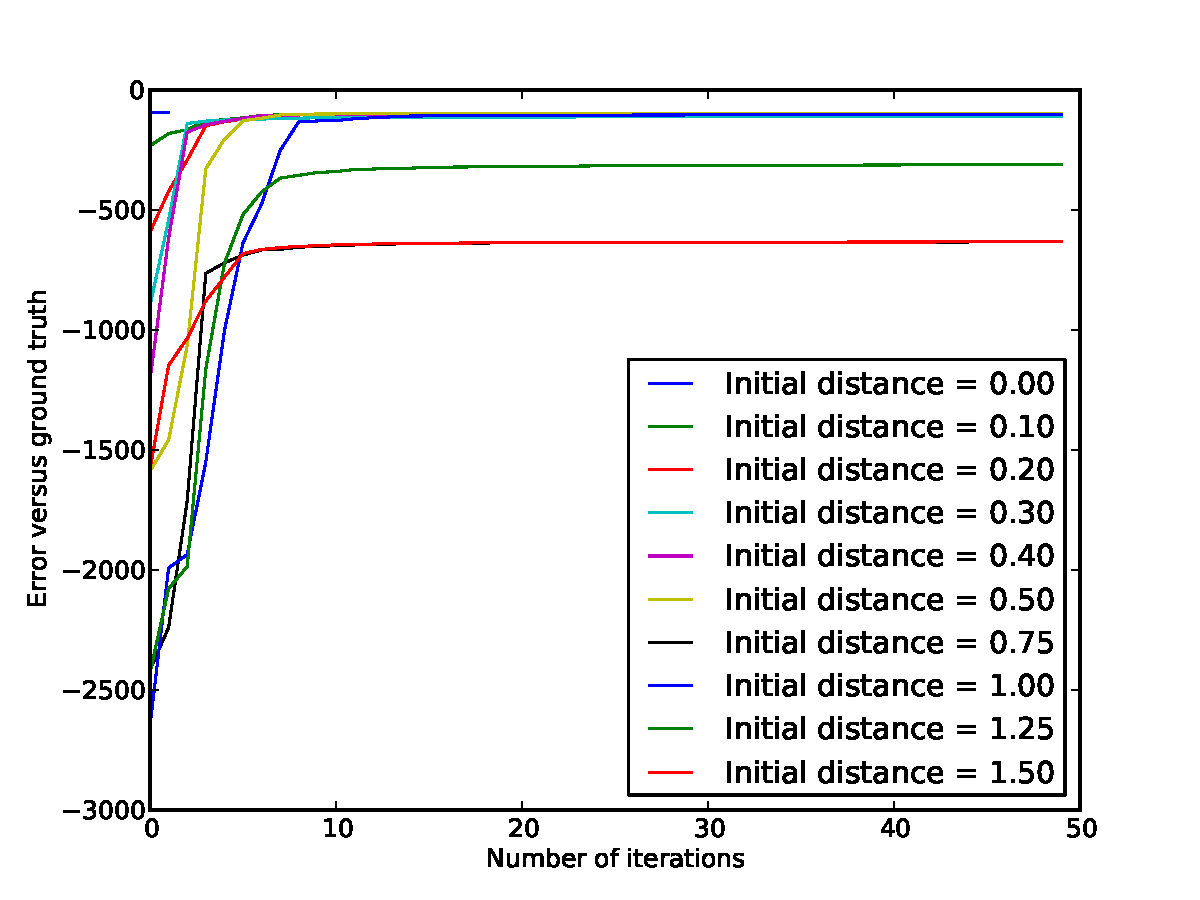
\includegraphics[width=0.65\textwidth]{plots/rotation_convergence_likelihood}
  }
  \caption{Illustration of the convergence properties of our gradient
    descent algorithm. We measure the distance from the estimated
    rotation to the ground truth after each gradient step. Each series
    above shows this evolution when our algorithm is initialised a
    particular distance from the ground truth. We see that for
    distances less than 1 convergence is robust. This corresponds to a
    large offset under the metric \eqnref{rotation-metric}, indicating
    that the optima has a wide basin of attraction. Note that for this
    experiment the labels $\Indicators$ are assumed known.}
  \label{fig:rotation-convergence}
\end{figure}

\begin{figure}[p]
  \centering
  \subfloat[Algebraic Estimate]{
    \includegraphics[width=0.46\textwidth]{new_vpt_comparison/exeter_bursary_frame23_vpts_algebraic}
  }\quad
  \subfloat[Normal--based Estimate]{
    \includegraphics[width=0.46\textwidth]{new_vpt_comparison/exeter_bursary_frame23_vpts_normals}
  }\\
  \subfloat[Single Image Estimate]{
    \includegraphics[width=0.46\textwidth]{new_vpt_comparison/exeter_bursary_frame23_vpts_singleimage}
  }\quad
  \subfloat[Geometric (Proposed) Estimate]{
    \includegraphics[width=0.46\textwidth]{new_vpt_comparison/exeter_bursary_frame23_vpts_geometric}
  }
  \caption{Comparison of rotation estimation algorithms for an example
    drawn from the ``Bursary'' sequence. Though only one frame is
    shown here, each algorithm other than (c) was provided with 7
    input frames.}
  \label{fig:vpt-example1}
\end{figure}

\begin{figure}[p]
  \centering
  \subfloat[Algebraic Estimate]{
    \includegraphics[width=0.46\textwidth]{new_vpt_comparison/exeter_mcr1_frame45_vpts_algebraic}
  }\quad
  \subfloat[Normal--based Estimate]{
    \includegraphics[width=0.46\textwidth]{new_vpt_comparison/exeter_mcr1_frame45_vpts_normals}
  }\\
  \subfloat[Single Image Estimate]{
    \includegraphics[width=0.46\textwidth]{new_vpt_comparison/exeter_mcr1_frame45_vpts_singleimage}
  }\quad
  \subfloat[Geometric (Proposed) Estimate]{
    \includegraphics[width=0.46\textwidth]{new_vpt_comparison/exeter_mcr1_frame45_vpts_geometric}
  }
  \caption{Comparison of rotation estimation algorithms for an example
    drawn from the ``MCR'' sequence. Though only one frame is
    shown here, each algorithm other than (c) was provided with 7
    input frames.}
  \label{fig:vpt-example2}
\end{figure}

\begin{figure}[p]
  \centering
  \subfloat[Algebraic Estimate]{
    \includegraphics[width=0.46\textwidth]{new_vpt_comparison/lab_ground1_frame21_vpts_algebraic}
  }\quad
  \subfloat[Normal--based Estimate]{
    \includegraphics[width=0.46\textwidth]{new_vpt_comparison/lab_ground1_frame21_vpts_normals}
  }\\
  \subfloat[Single Image Estimate]{
    \includegraphics[width=0.46\textwidth]{new_vpt_comparison/lab_ground1_frame21_vpts_singleimage}
  }\quad
  \subfloat[Geometric (Proposed) Estimate]{
    \includegraphics[width=0.46\textwidth]{new_vpt_comparison/lab_ground1_frame21_vpts_geometric}
  }
  \caption{Comparison of rotation estimation algorithms for an example
    drawn from the ``Ground1'' sequence. Though only one frame is
    shown here, each algorithm other than (c) was provided with 7
    input frames.}
  \label{fig:vpt-example3}
\end{figure}

%%%%%%%%%%%%%%%%%%%%%%%%%%%%%%%%%%%%%%%%%%%%%%%%%%%%%%%%%%%%%%%%%%%%%%
\section{Identifying The Vertical Direction}
Of the three dominant directions defined by $\SceneR$, two correspond to
horizontal directions and the third to the vertical direction. The
latter is semantically distinct since it defines the orientation of
the ground and ceiling planes, as well as the direction in which
gravity operates. It is easy to identify the vertical axis since
humans necessarily move over the ground plane when capturing video
sequences, and have limited scope for moving the camera in the
up--down direction. We therefore set the vertical axis to that over
which camera positions range the least. Having identified $\SceneR$ there
are only three possible choices, and we found this heuristic to work
correctly in all of our evaluation sequences.

%%%%%%%%%%%%%%%%%%%%%%%%%%%%%%%%%%%%%%%%%%%%%%%%%%%%%%%%%%%%%%%%%%%%%%
\section{Identifying The Floor And Ceiling Planes}
\label{sect:fcmap}

\begin{figure}[tb]
  \centering
  \subfloat[]{
    \includegraphics[width=0.4\textwidth]{manhattan-homology}
  }\quad
  \subfloat[]{
    \includegraphics[width=0.4\textwidth]{manhattan-homology-realworld}
  }
  \caption{\changedsinceviva{The mapping $\Hcf$ transfers points between the ceiling and
    floor in the image domain. $\Hcf$ is a planar homology.}}
  \label{fig:fcmap}
\end{figure}

An indoor Manhattan scene has exactly one floor and one ceiling plane,
both with normal $\vvpt$. It will be useful in the following chapters
to have available the mapping $\Hcf$ between the image locations of
ceiling points the floor points that are vertically below them (see
\figref{fcmap}). $\Hcf$ is a planar homology with axis
$\horizon=\lvpt\cross\rvpt$ and vertex $\vvpt$ \cite{Criminisi01} and
can be recovered given the image location of any pair of corresponding
floor/ceiling points $(\FloorPt,\CeilPt)$ as
\begin{equation}
  \Hcf = I + \mu\frac{\vvpt\horizon^T}{\vvpt \cdot \horizon} ~,
\end{equation}
where
\begin{equation}
  \mu = \bigl\langle\vvpt,\CeilPt,\FloorPt,
  \CeilPt\times\FloorPt\times\horizon\bigr\rangle
\end{equation}
is the characteristic cross ratio of $\Hcf$. Although we do not have
\textit{a priori} any such pair $(\FloorPt,\CeilPt)$, we can recover
$\Hcf$ using the following sampling algorithm. First we identify edges
in the image using one of the many available edge detection
algorithms. Next we sample one edge pixel $\vect{\hat{x}_c}$ from the
region above the horizon, then we sample a second point
$\vect{\hat{x}_f}$ collinear with the first and $\vvpt$ from the
region below the horizon. We then compute a hypothesis for $\Hcfhat$
as described above, and then assign a score by counting the number of
edge pixels that $\Hcfhat$ maps onto other edge pixels. After
repeating this for a fixed number of iterations we return the
hypothesis with greatest score.

Many images contain either no view of the floor or no view of the
ceiling. In such cases $\Hcf$ is unimportant since there are no
corresponding points in the image. If the best $\Hcf$ output from the
sampling process has a score below a threshold $k_t$ then we set $\mu$
to a large value that will transfer all pixels outside the image
bounds. $\Hcf$ will then have no impact on the estimated model.

In the context of multiple views we resolve scale by identifying
$\ScaleParam$ with either the maximum or minimum $z$ component of any
point in the point cloud reconstructed by structure--from--motion.

%% \subsection{Identifying the floor and ceiling planes.}
%% An indoor Manhattan scene has exactly one floor and one ceiling plane,
%% both with normal direction $\vvpt$. It will be useful in the following
%% sections to have available the mapping $\Hcf$ between the image
%% locations of ceiling points and the image locations of the floor
%% points that are vertically below them (see \figref{fcmap}). $\Hcf$ is
%% a planar homology with axis $\vect{h}=\lvpt\times\rvpt$ and vertex
%% $\vvpt$ \cite{Criminisi01} and can be recovered given the image
%% location of any pair of corresponding floor/ceiling points
%% $(\vect{x_f},\vect{x_c})$ as
%% \begin{equation}
%%   \Hcf = I + \mu\frac{\vvpt\vect{h}^T}{\vvpt \cdot \vect{h}} ~,
%% \end{equation}
%% where $\mu = \langle\vvpt,\vect{x_c},\vect{x_f},
%% \vect{x_c}\times\vect{x_f}\times\vect{h}\rangle$ is the characteristic cross
%% ratio of $\Hcf$.

%% Although we do not have \textit{a priori} any such pair
%% $(\vect{x_f},\vect{x_c})$, we can recover $\Hcf$ using the following
%% RANSAC algorithm. First, we sample one point $\vect{\hat{x}_c}$ from
%% the region above the horizon in the Canny edge map, then we sample a
%% second point $\vect{\hat{x}_f}$ collinear with the first and
%% $\vvpt$ from the region below the horizon. We compute the
%% hypothesis map $\Hcfhat$ as described above, which we then score by
%% the number of edge pixels that $\Hcfhat$ maps onto other edge pixels
%% (according to the Canny edge map). After repeating this for a fixed
%% number of iterations we return the hypothesis with greatest score.

%% Many images contain either no view of the floor or no view of the
%% ceiling. In such cases $\Hcf$ is unimportant since there are no
%% corresponding points in the image. If the best $\Hcf$ output from the
%% RANSAC process has a score below a threshold $k_t$ then we set $\mu$
%% to a large value that will transfer all pixels outside the image
%% bounds. $\Hcf$ will then have no impact on the estimated model.

\section{Extension: Relaxing The Manhattan World Assumption}
The strong Manhattan assumption states that any pair of surfaces of
interest are either parallel or orthogonal to one another. One common
deviation from this is scenes with walls that are orthogonal to the
floor and ceiling but not to one another. We define the weak Manhattan
assumption as ``the environment consists of a horizontal ground plane
and corresponding ceiling plane, and a set of vertical wall segments
extending continuously between them.'' Weakly Manhattan environments
contain much of the regularity of strongly Manhattan environments, and
here we discuss how to extending the approach taken in chapter to such
scenes. We have not implemented this approach; we discuss these ideas
as inspiration for future work.

We can deal with the weak Manhattan assumption as follows. First, we
run the EM algorithm described above to obtain $\SceneR$. Next, for
each line $\LineSeg_j$ marked as spurious by the EM algorithm we find
its intersection with the horizon,
\begin{equation}
  \vect{u}_j = \SceneR^{-T} R_i^{-T} \LineSeg_j \times \ez ~,
\end{equation}
which would be its vanishing point if it were horizontal in the
world. Vertical surfaces of a given orientation will generate
identical $\vect{u}_j$ (modulo measurement error), so we may identify
additional vertical orientations by clustering the intersections
$\{\vect{u}_j\}$. This should be possible even with few such
intersections, since the fact that all intersections are on the
horizon reduces this to a one--dimensional estimation problem.

%% We adopt a voting algorithm in which we parametrise
%% $\vect{u}_j$ in terms of the angle $\theta_j$ about the $z$ axis
%% \begin{equation}
%%   \theta_{j} = \mbox{atan}
%%   ({\ey}^T\vect{u}_j,~ {\ex}^T\vect{u}_j) ~.
%% \end{equation}
%% We accumulate the $\theta_j$ into histogram bins and identify any
%% local maxima $\theta_i^*$ above a threshold $k$. Each $\theta_i^*$
%% represents a cluster of line segments corresponding to an additional
%% vertical orientation. Finally, we re--estimate the vanishing point for
%% each cluster by minimising the likelihood \eqref{line-lik} via
%% least--squares.

\section{Conclusion}

We have proposed a principled approach to discovering the dominant
Manhattan directions given multiple calibrated views. Our likelihoods
are derived from a well--defined model of image generation, and we
solve inference as a single optimisation. Our work is strongly
influenced by the literature on vanishing point detection and our
approach parallels ideas previously proposed in the single--view
context. Our contribution is a principled way to incorporate multiple
calibrated views into a single optimisation, and an empirical
demonstration that doing so significantly out--performs both
single--view vanishing point estimation and surface--normal--based
estimators.


%%%%%%%%%%%%%%%%%%%%%%%%%%%%%%%%%%%%%%%%%%%%%%%%%%
%
\def\localpath{Inference}
\graphicspath{{\localpath/figures/}}
\chapter{Inference From Single and Multiple Views}
\label{chap:inference}
% If you like chapter abstracts ...
%\begin{quote}{\em This chapter describes an application of 

The abstract text is put into Ch\#/ab\#.tex, where
\# is the chapter number.
}\end{quote}
\begin{quote}
  This chapter addresses the recovery of indoor Manhattan models in
  the context of single and multiple views of a scene. We describe a
  Bayesian approach to reasoning about indoor Manhattan models in the
  face of ambiguous image evidence. To achieve this we present a
  graphical model that relates photometric cues, stereo
  photo--consistency, and depth cues to the scene model discussed in
  previous chapters. We show how to solve MAP inference using dynamic
  programming, allowing exact, global inference in $\sim$$100$ ms
  without using specialised hardware. Our approach is applicable to
  both the single-- and multiple--view settings by selecting various
  combinations of sensor models. Experiments show our system
  out--performing the state--of--the--art in the domain of indoor
  Manhattan reconstruction.\footnotemark
\end{quote}

\footnotetext{This work was published in part in:

{ \setlength{\parindent}{0pt} 
  \textit{Flint, Mei, Murray, and Reid,} ``A Dynamic Programming
  Approach To Reconstruction Building Interiors'', in \textit{Proceedings
    of the 2010 European Conference on Computer Vision}\cite{Flint10eccv}

  \textit{Flint, Murray, and Reid,} ``Manhattan Scene Understanding
  Using Monocular, Stereo, and 3D Features'', in \textit{Proceedings
    of the 2011 International Conference on Computer Vision}\cite{Flint11}
}
}

%%%%%%%%%%%%%%%%%%%%%%%%%%%%%%%%%%%%%%%%%%%%%%%%%%%%%%%%%%%%%%%%%%%%%%
\begin{figure}[tb]%
  \centering
    \includegraphics[width=0.45\textwidth]{firstpage/lab_foyer2_frame041_dp.jpg}
    \includegraphics[width=0.45\textwidth]{firstpage/exeter_mcr1_frame032_dp.jpg}
    \caption{Scene structure recovered by the system described in
      this chapter.}
  \label{fig:recovered-egs}
\end{figure}

\section{Introduction}
Over the past decade, computer vision researchers working with
monocular images have pursued substantially different research
agendas to those working with multiple views. The focus for
monocular images has increasingly been to infer high--level facts
about the world, such as the locations of and interactions between
objects, semantic scene categories, and the spatial layout of the
environment. In contrast, much of the work concerning multiple views
has focused on reconstructing metric scene structure and camera poses
using techniques such as structure--from--motion, stereo, and
multiple--view stereo.

In this chapter we leverage multiple view geometry for image
understanding purposes. We assume a moving camera with a
structure--from--motion system estimating its trajectory, and show how
to infer semantically meaningful models of the environment. We focus
on the \textit{indoor Manhattan
  representation}\cite{Lee09,Flint10eccv} that we described in
\chapref{geometry}.

Our approach is to define a probabilistic model that relates the
unknown scene layout to three types of observations: photometric image
features, stereo photo--consistency, and 3D point clouds. These three
quantities are commonly available in a moving camera setup, but our
system can be used unchanged with any combination of the three,
including a single--view setting. The second part of this chapter then
focuses on finding the most likely explanation for a set of
observations given the assumptions made by our model. A major focus of
this chapter is the development of an efficient and exact dynamic
programming that solves both maximum--aposteriori (MAP) and
maximum--likelihood (ML) inference in our model.

To present these two components (model and inference algorithm)
clearly, we begin by describing a class of optimisation problem that
we call the payoff formulation. This optimisation problem
provides the connection between the model we present first and
the inference algorithm we present second. In particular, we will show
during the development of the probabilistic model that MAP inference
can be written as an optimisation problem in payoff form. After we
have presented our model, we will thereafter be interested only in
solving general payoff--form problems, which allows us to decouple the
development of our dynamic programming algorithm from the specifics of
our probabilistic model --- we will simply show that we can solve all
optimisation problems in the payoff formulation. A further advantage
is that other sensor models that can be similarly reduced to payoff
form will also be amenable to our dynamic programming
algorithm. Although the presentation of an abstract class of
optimisation problem may seem an abstruse way to begin this chapter,
we believe that it leads to the clearest presentation overall.

%%%%%%%%%%%%%%%%%%%%%%%%%%%%%%%%%%%%%%%%%%%%%%%%%%%%%%%%%%%%%%%%%%%%%%
\section{The Payoff Formulation}

In this section we describe a class of optimisation problems that we
will refer to as the \textit{payoff formulation}. Throughout the
remainder of this chapter it will become clear that a range of
inference problems in the context of indoor Manhattan scenes can be
expressed in this form, and that this particular formulation permits a
general and efficient dynamic programming solution.

Let $\SetOfScenes$ be the set of indoor Manhattan scenes in vertex
representation. Let $\Scene\in\SetOfScenes$ be a scene in vertex
representation and let $\Seam$ be the corresponding scene in
seam representation. 

A payoff function $\PixelPayoff: \Dom\cross\SetOfOrientations
\Mapto\Reals$ maps integer pixel coordinates $\Pixel\in\Dom$ together
with orientations $\Orient\in\SetOfOrientations$ to real numbers. The
payoff for a scene $\Scene$ is defined in terms of the seam
representation,
\begin{equation}
  \label{eq:scene-payoff}
  \ScenePayoff(\Scene) = 
  \ScenePayoff(\Seam) =
  \sum_{j=1}^{\Width} \PixelPayoff(j,\seam_j,\WallOrient_j)
\end{equation}
where $\Seam = \{(\seam_j,\WallOrient_j)\}$. This sum consists of one
term for each image column. It is computed by adding together the
value of the payoff function at each pixel along the floor/wall seam
in $\Scene$. The form of the payoff function is problem--specific; all
we require is that it is a function of $j$, $\seam_j$, and
$\WallOrient_j$. Later we will describe specific payoff functions
$\PixelPayoff$ for the likelihoods in our model. In cases where the
payoff function is independent of $\WallOrient_j$ we will write
\begin{equation}
  \PixelPayoff(\Pixel) = \PixelPayoff(x,y,\cdot)
\end{equation}

Note that the value of $\PixelPayoff(\Pixel)$ is \textit{not}
restricted in any way to dependence on the image evidence at pixel
$\Pixel$, nor even to a local region about $\Pixel$; indeed, the
payoff functions described in the following sections incorporate image
evidence from widely separated image regions.

A penalty function $\ScenePenalty:\SetOfScenes\Mapto\Reals$ maps
scenes in the vertex representation to real numbers and takes the form,
\begin{equation}
  \label{eq:scene-penalty}
  \ScenePenalty(\Scene) = 
  \sum_{i=0}^{\NumWalls-1} \CornerPenalty(i;\Scene)
\end{equation}
where $\NumWalls$ is the number of walls contained in $\Scene$ and
$\CornerPenalty$ may be interpreted as a regulariser related to the
meeting between the $i$\th wall in $\Scene$ and its successor. Once
again, we have not defined any particular $\CornerPenalty$; any that
takes the the form \eqnref{scene-penalty} is suitable for the
optimisation problem to follow. Later we will describe specific forms
for $\CornerPenalty$ corresponding to particular choices of prior in
our model.

Given any such $\ScenePayoff$ and $\ScenePenalty$, the associated
optimisation problem is as follows. Let
\begin{eqnarray}
  \label{eq:scene-objective}
  \Objective(\Scene) &=&
  \ScenePayoff(\Scene) - \ScenePenalty(\Scene)\\
  &=&
  \sum_{j=1}^{\Width} \PixelPayoff(j,\seam_j,\WallOrient_j) -
  \sum_{i=0}^{\NumWalls-1} \CornerPenalty(i;\Scene) ~.
\end{eqnarray}
then we seek
\begin{equation}
  \label{eq:opt-scene}
  \OptimalScene = \argmax_{\Scene\in\SetOfScenes}\limits \Objective(\Scene) ~.
\end{equation}

Note that the objective $\Objective$ is defined partially in the scene
representation and partially in the vertex representation. This poses
no difficulty to evaluating $\Objective$ in the vertex representation
since we can readily obtain the seam representation via equation
\eqnref{seam-from-scene}. However, as discussed in
\secref{seam-representation}, the mapping from the vertex
representation to seam representation is not invertible, so the
objective above cannot be evaluated in the seam representation. For
this reason we will work in the vertex representation for the
presentation of the optimisation algorithm, but for convenience we
will work in seam representation to define  $\ScenePayoff$.

%%%%%%%%%%%%%%%%%%%%%%%%%%%%%%%%%%%%%%%%%%%%%%%%%%%%%%%%%%%%%%%%%%%%%%
\section{Probabilistic Model}

In this section we develop a probabilistic model for estimating indoor
Manhattan scenes from observations. We assume that three types of
observations are available: photometric image features, calibrated
stereo image pairs, and 3D point clouds. These quantities might be
acquired, for example, as the output of a SLAM or
structure--from--motion system. We now describe probabilistic
relationships between each type of observation and the indoor
Manhattan scene structure that we wish to infer.

%%%%%%%%%%%%%%%%%%%%%%%%%%%%%%%%%%%%%
\subsection{Scene Prior}

We turn first to the prior on scenes, $P(\Scene~|~\Penalties)$, which
is governed by a set of hyper--parameters $\Penalties$. As discussed in
\secref{corner-categories}, corners between successive walls can be
classified as concave, convex, or occluding. Let $n_1, n_2,$ and $n_3$
be the number of corners in $\Scene$ of each category
respectively. \changedsinceviva{Our prior on scenes is a geometric distribution in
$\vect{n}=(n_1,n_2,n_3)$,}
\begin{eqnarray}
  \label{eq:scene-prior}
  P(\Scene ~|~ \Penalties) &=& \frac{1}{Z}
    {\PenaltyConc}^{n_1} {\PenaltyConv}^{n_2} {\PenaltyOccl}^{n_3}~,
%  Z &=& \frac{\mu(n_1,n_2,n_3)}{(1-\PenaltyConc)(1-\PenaltyConv)(1-\PenaltyOccl)}~,
\end{eqnarray}
where $Z$ is a normalising term that we will not need to compute in
order to perform maximisation. Our choice of \eqnref{scene-prior} is
motivated by the desire to penalise scenes for additional complexity,
where we measure complexity by the number of distinct walls. We
discuss other priors, and some of the problems they raise in
\secref{other-priors}.

Taking logarithms yields
\begin{equation}
  \label{eq:log-scene-prior}
  \log P(\Scene ~|~ \Penalties) =
    -\log Z +
    n_1\log\PenaltyConc + 
    n_2\log\PenaltyConv + 
    n_3\log\PenaltyOccl~.
\end{equation}
Comparison with \eqnref{scene-penalty} suggests the following
penalty function:
\begin{equation}
  \label{eq:corner-penalty}
  \CornerPenalty(i;\Scene) = 
  \begin{cases}
    \log \PenaltyConc, &
      \mbox{if the $i$\th corner in $\Scene$ is concave} \\
    \log \PenaltyConv, &
      \mbox{if the $i$\th corner in $\Scene$ is convex} \\
    \log \PenaltyOccl, &
      \mbox{if the $i$\th corner in $\Scene$ is occluding} \\
  \end{cases}
\end{equation}
The cases above can be decided by the algorithm described in
\secref{corner-categories}. Substituting \eqnref{corner-penalty} into
\eqnref{scene-penalty} yields
\begin{equation}
  \ScenePenalty(\Scene) = \log P(\Scene ~|~ \Penalties) + \log Z~.
\end{equation}
We can safely ignore the constant term since our ultimate goal is the
optimisation expressed in \eqnref{opt-scene}.

%%%%%%%%%%%%%%%%%%%%%%%%%%%%%%%%%%%%%
\subsection{Photometric Sensor Model}

We now introduce a model relating indoor Manhattan scenes to observed
image features. We begin with the single--view scenario in which we
observe a feature $\Feature\in\Reals^n$ at each pixel $\Pixel$.

\begin{figure}[tb]
  \centering
  \includegraphics[width=0.6\textwidth]{monocular-gm}
  \caption{The graphical model relating scenes $\Scene$ to monocular
    image features $\Feature$. $\Pixel=(x,y)$ is a pixel location and
    $a$ is the orientation predicted (deterministically) by $\Scene$
    at $\Pixel$.}
  \label{fig:photometric-gm}
\end{figure}

We assume the graphical model shown in \figref{photometric-gm}. The
generative process begins by sampling a scene $\Scene$, then samples
pixels $\Pixel$ and computes their orientation
$\Orient\in\Orientations$ (\cf
\algref{computing-from-scene}), which is deterministic given $\Scene$
and is included in the graphical model for notational convenience
only. Finally a feature $\Feature$ is sampled from a distribution that
is conditionally independent of $\Scene$ given $\Orient$. \changedsinceviva{In practice
we use the following features: three RGB colour components,
three HSV colour components, two binary line sweep features described
by Lee \etal \cite{Lee09}, and twelve Gabor responses (three scales,
four orientations). In \chapref{learning} we drop the
Gabor responses for efficiency reasons.
}

We assume a exponential--family likelihood for pixel features,
\begin{equation}
  \label{eq:pixel-likelihood}
  P(\Feature ~|~ \Orient) \propto
    \exp(\PixelModel_\Orient \cdot \Feature) ~.
\end{equation}

Denoting the set of all observed pixel
features $\Features$, pixels $\Pixels$, and orientations $\Orients$,
the joint distribution is
\begin{equation}
  P(\Features, \Pixels, \Orients, \Scene, \Penalties, \PixelModel) =
    P(\Scene ~|~ \Penalties) 
    \prod P(\Pixel_i)
          P(\Orient_i ~|~ \Scene, \Pixel_i)
          P(\Feature_i ~|~ \Orient_i, \PixelModel) ~.
\end{equation}
We do not model the distribution $P(\Pixel_i)$ and for the remainder
of this section it may be assumed that all probabilities are
conditioned on this quantity.

We now derive MAP inference. The likelihood for $\Scene$ is
\begin{equation}
  \label{eq:photometric-lik-full}
  P(\Features ~|~ \Scene) \propto 
  \int
    \prod_i P(\Feature_i ~|~ \Orient_i) 
            P(\Orient_i ~|~ \Scene)
  \intd \Orients ~.
\end{equation}
In the integration over the latent variables, the only
non--zero term is the one for which all $\Orient_i$ are equal to that
predicted by \algref{computing-from-scene}. Therefore, denoting by
$\PredictedOrient_i$ the orientation output by
\algref{computing-from-scene} for pixel $\Pixel_i$ under $\Scene$ we
have
\begin{equation}
  \label{eq:photometric-lik}
  P(\Features ~|~ \Scene) \propto
    \prod_i P(\Feature_i ~|~ \PredictedOrient_i) ~.
\end{equation}
Taking logarithms gives
\begin{equation}
  \label{eq:photometric-loglik}
  \log P(\Features ~|~ \Scene) =
    \sum_i \log P(\Feature_i ~|~ \Orient_i^*) + c
\end{equation}
where $c$ corresponds to the constant of proportionality in
\eqnref{photometric-lik}, which we henceforth drop since it makes no
difference to the optimisation to come. 

At this point we use the crucial observation of
\secref{col-decomposability} that the orientation
$\PredictedOrient_i$ is functionally dependent only on the pair
$(\seam_j,\WallOrient_j)$ for the column $j$ containing
$\Pixel_i$. Let $\ComputedOrient(x,y;\seam_j,\WallOrient_j)$ be the
orientation output by \algref{computing-from-scene} for pixel $(x,y)$
under the hypothesis $(\seam_j,\WallOrient_j)$. We define
\begin{equation}
  \label{eq:mono-payoffs}
  \MonoPayoff(x,y,\WallOrient) = \sum_{r=0}^H \log 
    P(\Feature_{xr} ~|~ \ComputedOrient(x,r;y,\WallOrient)~)
\end{equation}
where the double--subscript in $\Feature_{xr}$ is a result of
separately indexing rows and columns in \eqnref{mono-payoffs}. 

Now consider the scene payoff,
\begin{eqnarray}
  \ScenePayoff(\Scene) &=& 
    \sum_{j=0}^W \MonoPayoff(j, \seam_j, \WallOrient_j) \\
  &=& 
    \sum_{j=0}^W \sum_{r=0}^H \log
      P(\Feature_{jr} ~|~ \ComputedOrient(j,r;\seam_j,\WallOrient_j)~)\\
  &=&
    \log P(\Features ~|~ \Scene) + O(1)  ~.
    \label{eq:photometric-in-scene-payoff}
\end{eqnarray}
This is simply the log--likelihood \eqnref{photometric-loglik} up to a
constant, so maximising \eqnref{photometric-in-scene-payoff} is
equivalent to maximising \eqnref{photometric-loglik}. In this sense we
have placed our model in the payoff formulation outlined in the
previous section since by substituting the particular payoff function
$\MonoPayoff$ into \eqnref{opt-scene} we obtain an optimisation
problem in payoff formulation that is equivalent to
maximum--likelihood inference under the graphical model of
\figref{photometric-gm}. (Later we will show that this result extends
easily to MAP inference also.)

%%%%%%%%%%%%%%%%%%%%%%%%%%%%%%%%%%%%%
\subsection{Multiple--View Sensor Model}

\begin{figure}[tb]
  \centering \includegraphics[width=0.8\textwidth]{backproject}
  \caption{Pixel correspondences across multiple views are computed by
    back--projection onto the model $\Scene$ followed by re--projection into
    auxiliary views.}
  \label{fig:backproject}
\end{figure}
We now formulate the payoff function $\StereoPayoff$ for the case that
multiple views of the scene are available. We assume \changedsinceviva{that one}
image is identified as the base view $\Image_0$; the remaining
$\NumViews$ images are denoted
$\Image_1,\ldots,\Image_{\NumViews}$. All images have size
$\Width\times\Height$. We assume that all cameras are calibrated with
the action of the $i$\th camera on a 3D point $X$ being
\begin{equation}
  \CamMatrix_i (\CamR_i X + \CamTr_i) ~.
\end{equation}

Intuitively, we treat inference in this settings as follows. We
consider models $\Scene$ in terms of their projection into
$\Image_0$. We explained in \secref{model} that models parametrised in
image coordinates specify unique 3D models. Any model hypothesised in
$\Image_0$ can therefore be re--projected into the auxiliary views,
giving pixel--wise correspondences between frames (\cf
\figref{backproject}). From this we compute a photo--consistency
measure $\pc(\cdot)$, which provides the likelihood $P(\StereoData ~|~
\Scene)$.

Optimising over photo--consistency has been standard in the stereo
literature for several decades \cite{Scharstein01}; our contribution
is to show that (i) in the particular case of indoor Manhattan models,
photo--consistency can be expressed as a payoff matrix; (ii) that we
can therefore perform efficient and exact global optimisation; and
(iii) that this fits naturally within a Bayesian framework alongside
monocular and 3D features. \changedsinceviva{Our approach also bears some similarity to
Cornelis \etal \cite{Cornells2006}, who reconstruct building facades
from a moving vehicle by analysing a related cost function derived
from stereo pairs. Like us, they employ dynamic programing, although
they do not constrain the arrangement of the vertical facades.
}

In \secref{metric-recovery} we showed how to convert a scene in vertex
representation to a 3D reconstruction. Since all cameras are
calibrated we can use this reconstruction to re--project any pixel
$\Pixel$ from the base view into all auxiliary views, as illustrated in
\figref{backproject}. Let $\AuxPixel_k(\Pixel;\Scene)$ be the
re--projection of $\Pixel$ into view $k$ via the scene hypothesis
$\Scene$. Let each pixel $\Pixel_i$ in the base image be associated
with a feature vector $\Feature_i\in\Reals^n$ and let each pixel
$\AuxPixel_{ki}$ in the $k$\th auxiliary view be similarly associated
with a feature $\AuxFeature_{ki}\in\Reals^n$. Let $\Features$ be the
set of all features in the base view and let $\AuxFeatures_k$ be the
set of all features in the $k$\th auxiliary view. Finally, let
\begin{equation}
  \ComputedAuxFeature_k(\Pixel_i;\Scene) =
  \AuxFeature(\AuxPixel_k(\Pixel_i;\Scene))
\end{equation}
be the feature associated with the reprojection of $\Pixel_i$ into the
$k$\th auxiliary view under the scene hypothesis $\Scene$. Then the
likelihood for $\Scene$ under our model is
\begin{equation}
  P(\Features,\AuxFeatures_1,\ldots,\AuxFeatures_K ~|~ \Scene) =
    \prod_i \prod_{k=0}^{\NumViews} 
      P(\Feature_i, \ComputedAuxFeature_k(\Pixel_i;\Scene) ~|~
      \StereoCov)~.
  \label{eq:stereo-likelihood}
\end{equation}
and following the standard approach \cite{Scharstein01}, the feature
likelihood is a zero--mean Gaussian:
\begin{equation}
  P(\Feature_i, \ComputedAuxFeature_k(\Pixel_i;\Scene) ~|~ \StereoCov)
   = \NormalDistr(\Feature_i-\ComputedAuxFeature_k(\Pixel_i;\Scene); \StereoCov)
\end{equation}

Taking logarithms we recognise a simple sum over pixel--wise
photo--consistency terms,
\begin{equation}
  \label{eq:stereo-loglik}
  \log P(\Features,\AuxFeatures_1,\ldots,\AuxFeatures_{\NumViews}
            ~|~ \Scene) =
  \sum_i \sum_{k=0}^{\NumViews} 
    \|\Feature_i-\ComputedAuxFeature_k(\Pixel_i;\Scene)\|_{\StereoCov}
   +c
\end{equation}

\begin{figure}[tb]
  \centering \includegraphics[width=0.8\textwidth]{reprojected-columns}
  \caption{Two hypotheses for the location of the seam and the
    reprojections they imply for each image column in an auxiliary
    image. The blue dot happens to be a correct hypothesis (unbeknown
    to the system), while the red dot is incorrect. As a result, the
    blue line corresponds to the same set of 3D locations in both
    images but the red line does not.}
  \label{fig:reprojected-columns}
\end{figure}

We now write equation \eqnref{stereo-loglik} in payoff form. To this
end we leverage the observation made in \secref{col-decomposability}
that the depth of a pixel $\Pixel$ under a scene hypothesis $\Scene$
is functionally dependent only on the pair $(\seam_j,\WallOrient_j)$
for the column $j$ containing $\Pixel$. Let
$\ComputedDepth(\Pixel;\seam_j)$ be the depth of $\Pixel$ under
the hypothesis $\seam_j$, as output by \algref{seam-depth-orient}.

Furthermore, re--projecting a pixel into an auxiliary view requires
only the depth at that pixel. Therefore we can identify all
correspondences for any pixel $\Pixel$ from the value $\seam_j$
alone. Specifically, the re--projection of $\Pixel$ into the $k$\th
view under the hypothesis $\seam_j$ is
\begin{equation}
  \AuxPixel_k(\Pixel;\seam_j) = \CamMatrix_k (\CamR_k X_i + \CamTr_k)
\end{equation}
where
\begin{equation}
  X_i = 
  \CamR_0^{-1} \bigl(
    \bar{\Depth}(\Pixel;\seam_j) \CamMatrix_0^{-1} \Pixel - \CamTr_0
  \bigr) ~.
\end{equation}
We can now re--write the correspondence function
$\ComputedAuxFeature_{ki}$ in terms of $\seam_j$ alone,
\begin{equation}
  \ComputedAuxFeature_k(\Pixel;\seam_j) = 
    \AuxFeature(\AuxPixel_k(\Pixel;\seam_j)) ~.
\end{equation}
Finally, the payoff function is
\begin{equation}
  \label{eq:stereo-payoffs}
  \StereoPayoff(x,y) = \sum_{r=0}^H \sum_{k=1}^{\NumViews}
    \| \Feature_{xr} - \ComputedAuxFeature_k([x,r]^T;y) \|_\Sigma
\end{equation}
where as in \eqnref{mono-payoffs} we have switched to a separate
indexing scheme for rows and columns, so $\Feature_{xy}$ is the
feature for the pixel at $(x,y)$ and $\ComputedAuxFeature_k(x,r;y)$
the the feature for the reprojection of $(x,r)$ into the $k$\th view
under the hypothesis $\seam_j=y$. Substituting \eqnref{stereo-payoffs}
into \eqnref{scene-payoff},
\begin{eqnarray}
  \ScenePayoff(\Scene) &=& 
    \sum_{j=0}^W \StereoPayoff(j,\seam_j)\\
  &=&
    \sum_{j=0}^W \sum_{r=0}^H \sum_{k=1}^{\NumViews}
    \| \Feature_{jr} - \ComputedAuxFeature_k([j,r]^T;\seam_j) \|_\Sigma\\
  &=&
    \log P(\Features,\AuxFeatures_1,\ldots,\AuxFeatures_{\NumViews}
             ~|~ \Scene) - c
\end{eqnarray}

The completes the reduction of the stereo sensor model to payoff form,
since we have shown that maximising the likelihood
\eqnref{stereo-likelihood} is equivalent to the payoff optimisation
problem \eqnref{opt-scene} for a particular instantiation of the payoff
function $\PixelPayoff$.

\subsubsection{A Different View}

Our approach could also be cast as solving the general stereo problem
in terms of disparity maps, where in place of priors based on
pixel--wise smoothness constraints, our prior is \eqnref{scene-prior}
for those disparity maps that correspond to valid indoor Manhattan
reconstructions, and zero for others. Inference under this model would
be intractable if cast directly in terms of disparity maps because
determining whether a given disparity map corresponds to some indoor
Manhattan reconstruction is difficult. Nevertheless, our approach
shows that by re--parametrising in the vertex representation the
problem becomes tractable.

Note that the column--wise decomposition \eqnref{stereo-payoffs}
neither commits us to optimising over columns independently, nor to
ignoring interactions between columns. By inspecting
\eqnref{stereo-likelihood} one sees immediately that our model assumes
no independence between image columns (only conditional independence
given $\Scene$), and indeed correlations do come into effect when we
optimise over the full payoff matrix later in this chapter.  Our
results will show that widely separated image regions often interact
strongly. The derivations in this section follow deductively from the
indoor Manhattan assumption; the only approximation is that concerning
occlusions, which we discuss below.

\subsubsection{Occlusions}

We have ignored self--occlusions in \eqnref{stereo-likelihood}. For
short baselines, such as frames sampled over a few seconds from a
moving camera, this is unproblematic since indoor environments tend to
be mostly convex from any single point of view. Even in highly
non--convex environments our system achieves excellent results by
integrating 3D and monocular features, and enforcing strong global
consistency, as will be shown in our experimental section. Further
discussion of this issue is in the final section of this chapter.

%%%%%%%%%%%%%%%%%%%%%%%%%%%%%%%%%%%%
\subsection{Point Cloud Sensor Model}

\begin{figure}[tb]
  \centering
  \includegraphics[width=0.6\textwidth]{3d-gm}
  \caption{The graphical model relating indoor Manhattan models to 3D
    points. The hidden variable $t$ indicates whether the point is
    inside, outside, or coincident with the model.}
  \label{fig:3d-gm}
\end{figure}

In this section we explore the context in which a 3D point cloud is
available during inference. The point clouds generated by
structure--from--motion systems are typically too sparse for direct
reconstruction, but can provide useful cues alongside monocular and
stereo data.

\begin{figure}[tb]
  \centering \includegraphics[width=0.8\textwidth]{point-projs}
  \caption{Depth measurements $d_i$ might be generated by a surface in
    our model (represented by $t_i=\ON$) or by an object inside or
    outside the environment (in which case $t_i=\IN,\OUT$
    respectively).}
  \label{fig:point-projs}
\end{figure}


%For each pixel $\Pixel_i$ a depth measurement $d_i$ is made. The
%relationship between $d$ and the model $M$ is determined by a hidden
%variable $t\in\{\textsf{IN},\textsf{ON},\textsf{OUT}\}$, which is
%interpreted as follows. Let $\DepthAtPGivenModel$ be the true depth of
%the model $\Scene$ in the direction $\Pixel$. If $t=\textsf{IN}$ then
%$\Depth$ corresponds to an object inside the room,

Our graphical model for 3D data is depicted in \figref{3d-gm}. The
model $\Scene$ is sampled according to the prior \eqnref{scene-prior},
then depth measurements $d_i$ are generated for pixels
$\Pixel_i$. Many such measurements will correspond to clutter or
measurement errors, rather than to the walls represented by
$\Scene$. Our model captures this uncertainty explicitly through
the latent variable $t_i$, which has the following interpretation. If
$t_i=\ON$ then $d_i$ corresponds to some surface represented
explicitly in $\Scene$. Otherwise, either $t_i=\IN$, meaning some
clutter object within the room was measured, or $t_i=\OUT$, in which
case an object outside the room was measured, such as through a
window. The likelihoods we use are
\begin{align}
  \label{eq:x-inside}
  P(\Depth~|~\Pixel,\Ind=\textsf{IN},\Scene) &=
  \begin{cases}
    \alpha, & \mbox{if } 0 < \Depth < \DepthAtPGivenModel \\
    0, & \mbox{otherwise} \\
  \end{cases} \\
  \label{eq:x-outside}
  P(d~|~\Pixel,\Ind=\textsf{OUT},\Scene) &=
  \begin{cases}
    \beta, & \mbox{if } \DepthAtPGivenModel < \Depth < \Dmax \\
    0, & \mbox{otherwise} \\
  \end{cases} \\
  P(\Depth ~|~ \Pixel,\Ind=\textsf{ON},\Scene) &=
  \NormalDistr(\Depth~;~\DepthAtPGivenModel,\sigma) ~.
\end{align}
where $\alpha$ and $\beta$ are determined by the requirement that the
probabilities sum to $1$ and $\DepthAtPGivenModel$ denotes the depth
predicted by $\Scene$ at $\Pixel$. We compute likelihoods on $\Depth$ by
marginalising over $\Ind$,
\begin{align}
  \label{eq:3d-likelihood}
  P(\Depth~|~\Pixel,\Scene,\IndModel) &=
   \sum_{\Ind} P(\Depth~|~\Pixel,\Scene,\Ind) P(\Ind~|~\IndModel)
  ~.
\end{align}
where $P(\Ind~|~\IndModel)$ is a categorical distribution with
parameters $\tIN$, $\tOUT$, and $\tON$. Equation
\eqnref{3d-likelihood} can be readily evaluated for any $\Depth$ and
$\Pixel$ since the sum is over just the three possible values for
$\Ind$. Denoting the set of all depth measurements $\Depths$, the full
likelihood for $\Scene$ is
\begin{eqnarray}
  \label{eq:depth-loglik}
  P(\Depths ~|~ \Pixels,\Scene) &=&
    \prod_i P(\Depth_i ~|~ \Pixel_i,\Scene)\\
  \log P(\Depths ~|~ \Pixels,\Scene) &=&
    \sum_i \log P(\Depth_i ~|~ \Pixel_i,\Scene)
\end{eqnarray}
We now utilise the same observation as we did in the previous section,
namely that the depth at $\Pixel$ is functionally dependent only on
the seam pair in the column containing $\Pixel$. Retaining the
notation under which $\ComputedDepth(\Pixel;\seam_j)$ is the depth at
$\Pixel$ computed by \algref{seam-depth-orient} for $\Scene$, we
define the payoff function
\begin{equation}
  \label{eq:depth-payoffs}
  \DepthPayoff(x,y) = 
  \sum_{i\in\Depths_x} \log P(\Depth_i~|~\Pixel_i,\ComputedDepth(\Pixel_i;y))
\end{equation}
where $\Depths_x$ contains indices for all depth measurements in
column $x$. We verify that \eqnref{depth-payoffs} does in fact
correspond to the log--likelihood \eqnref{depth-loglik} by
substituting the above into \eqnref{scene-payoff}, giving
\begin{eqnarray}
  \ScenePayoff(\Scene) &=& 
    \sum_{j=0}^W \DepthPayoff(j,\seam_j)\\
  &=&
    \sum_{j=0}^W \sum_{i\in\Depths_j} 
    \log P(\Depth_i~|~\Pixel_i,\ComputedDepth(\Pixel_i;\seam_j)~)\\
  &=&
    \log P(\Depths ~|~ \Pixels, \Scene)~.
\end{eqnarray}

%%%%%%%%%%%%%%%%%%%%%%%%%%%%%%%%%%%%
\subsection{Joint Model}
We combine photometric, stereo, and 3D data into a joint model by
assuming conditional independence given $\Scene$,
\begin{equation}
  P(\Observations_{\textsf{mono}}, \Observations_{\textsf{stereo}}, \Observations_{\textsf{3D}} ~|~ \Scene)
  =
    P(\Observations_{\textsf{mono}} ~|~ \Scene)
    P(\Observations_{\textsf{stereo}} ~|~ \Scene)
    P(\Observations_{\textsf{3D}} ~|~ \Scene) ~.
  \label{eq:full-posterior}
\end{equation}
Taking logarithms leads to summation over payoffs,
\begin{equation}
  \log P(\Observations_{\textsf{mono}}, \Observations_{\textsf{stereo}}, \Observations_{\textsf{3D}} ~|~ \Scene)
  = \ScenePayoff_{\textsf{joint}}(\Scene)
\end{equation}
where
\begin{equation}
  \JointPayoff(\Pixel) =
  \MonoPayoff(\Pixel) + 
  \StereoPayoff(\Pixel) +
  \DepthPayoff(\Pixel) ~.
\end{equation}
Finally, the log posterior is
\begin{equation}
  \begin{split}
    \log P(\Scene ~|~
           \Observations_{\textsf{mono}},
           \Observations_{\textsf{stereo}},
           \Observations_{\textsf{3D}})
    & \propto
      \log P(\Observations_{\textsf{mono}} ~|~ \Scene)
      +\log P(\Observations_{\textsf{stereo}} ~|~ \Scene) \\
    & \qquad + \log P(\Observations_{\textsf{3D}} ~|~ \Scene) + \log P(\Scene)\\
    & \propto \ScenePayoff_{\textsf{joint}}(\Scene) - \ScenePenalty(\Scene)~.
  \end{split}
  \label{eq:joint-posterior}
\end{equation}
The relation above is a proportionality rather than an equality
because we have omitted the evidence $P(\Observations)$. For the
purpose of maximisation this term is irrelevant since it is
independent of the quantity that we are maximising. We can now cast
maximum--likelihood and maximum--aposteriori inference in the form
\eqnref{scene-objective},
\begin{eqnarray}
  \OptimalScene_{\mbox{\tt ML}} &=& 
    \argmax_{\Scene\in\SetOfScenes}\limits~
    \ScenePayoff_{\textsf{joint}}(\Scene)\\
  \OptimalScene_{\mbox{\tt MAP}} &=& 
    \argmax_{\Scene\in\SetOfScenes}\limits~
    \ScenePayoff_{\textsf{joint}}(\Scene) - \ScenePenalty(\Scene) ~.
\end{eqnarray}

This completes the task of writing inference for our model in payoff
form. In particular, the above derivations show that for any set of
observations (photometric, stereo, depth, or any combination thereof),
there is a particular payoff function $\ScenePayoff$ and penalty
function $\ScenePenalty$ such that solving \eqnref{opt-scene} is
equivalent to solving MAP (or ML) inference under our model. In
practice we only need to evaluate $\ScenePayoff$ at integer pixel
coordinates, so we represent it as a 2D array. The remainder of this
chapter focuses on solving optimisation problems of the form
\eqnref{opt-scene}.


%%%%%%%%%%%%%%%%%%%%%%%%%%%%%%%%%%%%%%%%%%%%%%%%%%%%%%%%%%%%%%%%%%%%%%
\section{MAP Inference Using Dynamic Programming}

In this section we solve the optimisation problem
\eqnref{opt-scene}. That is, given some $\PixelPayoff$ and
$\CornerPenalty$, we wish to identify the maximiser $\OptimalScene$ of
\begin{equation}
  \Objective(\Scene) =
    \sum_{j=1}^{\Width} \PixelPayoff(j,\seam_j,\WallOrient_j) -
    \sum_{i=0}^{\NumWalls-1} \CornerPenalty(i;\Scene) ~,
\end{equation}
where
\begin{equation}
  \Scene =
  ( x_1,y_1,\WallOrient_1,
   ~x_2,y_2,\WallOrient_2,
   ~\ldots,
   ~x_{n-1},y_{n-1},\WallOrient_{n-1}, ~x_n )
\end{equation}
is an indoor Manhattan scene in vertex representation.

We assume that the scene rotation $\SceneR$ as well as the Manhattan
homology $\Hcf$ have been recovered as discussed in
previous chapters. We further assume that all images are rectified
as in \eqnref{rectification}. The algorithms presented in this section
are valid without the rectification step, but assuming rectification
considerably simplifies their presentation. Our solution uses dynamic
programming to efficiently solve the maximisation
\eqnref{opt-scene}. We develop the algorithm conceptually before
formalising it.

In the optimisation \eqnref{opt-scene}, we wish to constrain solutions
to valid indoor Manhattan scenes. In terms of individual pixel labels,
such a constraint introduces complicated dependencies between large
groups of pixels, since assigning a particular label to any one pixel
restricts which labels can be assigned to other pixels in the same
column. We therefore cast the optimisation directly in terms of the
vertex representation introduced in \chapref{geometry}.

We present our solution by first describing a simple but inefficient
version, followed by three refinements that lead to an $O(N)$
algorithm (where $N$ is the number of pixels). At each stage we
describe our algorithm conceptually before formalising it.

\subsection{Basic Algorithm}
\label{sec:basic-alg}

We have already seen that every indoor Manhattan scene can be
represented as a left--to--right sequence of wall segments. Our
approach is based on the construction of a graph over all possible
indoor Manhattan scenes. This nodes in this graph represent pixels and
the edges represent vanishing lines. Each path in this graph
corresponds to a different indoor Manhattan scene, and by assigning
certain weights to the edges we reduce the optimisation problem
\eqnref{opt-scene} to a graph search problem, which we solve using
dynamic programming. The graph is depicted informally in
\figref{dp-search-graph}. In dynamic programming parlance, nodes are
called states and the adjacency matrix is called the feasible set. We
now describe the construction of this graph.

\textbf{State space.} Our state space contains two states for each
pixel. Each state corresponds to a sub--problem of the form,
\textit{``What is the optimal indoor Manhattan scenes spanning the
  part of the image to the left of pixel $\Pixel$?''}. There is
one state for each pixel and each for of the two vertical
orientations, giving the $2N$ state space. We write states as pairs,
as in $\State=(\Pixel,\WallOrient)$.

\textbf{Feasible set.} The feasible set describes the connections
between states. There is a separate feasible set
$\FeasibleSet(\State)$ for each state and
$\OtherState\in\FeasibleSet(\State)$ if and only if there is an edge
from $\State$ to $\OtherState$. In our first algorithm the feasible
set for a state $\State=(\Pixel,\WallOrient)$ consists of all pixels
to the left of $\Pixel$ that fall on the vanishing line connecting
$\Pixel$ and $\vpt_{\WallOrient}$, as depicted in
\figref{dp-search-graph}. This leads to a search graph in which each
path corresponds to an indoor Manhattan scene, as shown in
\figref{path-correspondence}.

\textbf{Value function.} The value function describes the quantity
being optimised at each state. Our value function maps \textit{paths
  through the graph} to real numbers. That is, the domain of our value
function is the set of paths from any pixel $\Pixel$ to the left edge
of the image. We define the value of such a path to be the sum of the
entries in the payoff matrix along the path minus the penalty for the
corners along the path, \ie
\begin{equation}
  \Objective(\PartialScene) = \sum
    \PixelPayoff(j,\seam_j,\WallOrient_j) -
    \sum_{i=0}^{\SceneLen} \CornerPenalty(i;\PartialScene) ~.
  \label{eq:scene-value}
\end{equation}
\figref{partial-seam} shows one such path and the elements of the
payoff matrix that are summed to compute its value. The motivation for
choosing this particular value function is that for pixels on the
right edge of the image it is equal to the full objective function
\eqnref{opt-scene}.

\begin{figure}[tb]
  \centering
  \includegraphics[width=0.35\textwidth]{path-correspondence}
  \caption{A path through the search graph and the indoor Manhattan
    scene that it corresponds to. The black dots are states, the red
    arrows are edges, and the rest is for illustration only.}
  \label{fig:path-correspondence}
\end{figure}

\begin{figure}[tb]
  \centering
  \includegraphics[width=0.5\textwidth]{dp-search-graph}
  \caption{The search graph corresponding to the first version of our
    dynamic programming algorithm. This figure identifies one node
    (red circle) and shows all neighbours to which it is connected via
    outgoing edges (grey circle).}
  \label{fig:dp-search-graph}
\end{figure}

\begin{figure}[tb]
  \centering
  \includegraphics[width=0.35\textwidth]{partial-seam}
  \caption{A path from the left edge of the image to a particular
    state $\State$. The value of this path is the sum of all entries
    in the payoff matrix along the path highlighted in red.}
  \label{fig:partial-seam}
\end{figure}

\textbf{Optimisation step.} We now show how to maximise the value
function at each state. This is best explained by considering a single
state $\State$ and assuming that we already know the solutions for all
preceding states --- that is, for each state $\OtherState$ to
the left of $\State$, let us assume that we already know the
optimal\footnote{Optimality here means the path that maximises the
  value function described above.}
path from $\OtherState$ to the left edge of the image, and also the
value of that path. We denote this quantity
\begin{equation}
  \label{eq:bestvalue-def}
  \bestvalue(\OtherState) = \argmax \Objective(\Scene)
\end{equation}
where the maximisation is over paths terminating at $\OtherState$. Our
task is to use the known solutions to the preceding states to
discover the optimal path for the state $\State$ under
consideration. We accomplish this as follows.
\begin{enumerate}
  \item{Enumerate all states $\OtherState$ that are connected to
    $\State$; \ie all $\OtherState\in\FeasibleSet(\State)$.
  }
  \item{For each, compute
    \begin{equation}
      \label{eq:optimisation-step}
      \bestvalue(\OtherState)+\edgevalue(\OtherState,\State) ~,
    \end{equation}
    where
    \begin{equation}
      \label{eq:edge-value-basic}
      \edgevalue(\OtherState,\State) =
        \sum \PixelPayoff(x_i,y_i,\WallOrient_i) - \CornerPenalty
    \end{equation}
    is the sum of payoffs along the line segment between
    $\OtherState$ and $\State$, and $\Penalty$ is the penalty
    associated with the new corner at $\OtherState$ (see
    \figref{recurrence-value}). $\edgevalue$ can be thought of as the
    marginal value for the wall segment added between $\OtherState$
    and $\State$.
  }
  \item{Set $\bestvalue(\State)$ to the maximum over the terms
    computed in step 2. We summarise this in the following recurrence
    relation.
    \begin{equation}
      \bestvalue(\State) = 
      \max_{\OtherState \in \FeasibleSet(\State)}\limits
      \bestvalue(\OtherState) + \edgevalue(\OtherState,\State)
    \end{equation}
  }
\end{enumerate}

\begin{figure}[tb]
  \centering
  \includegraphics[width=0.35\textwidth]{recurrence-value}
  \caption{The computation of the value function at $\State$. This
    figure shows just one term in the maximisation
    $\eqnref{optimisation-step}$; computing $\bestvalue(\State)$
    involves maximisation over all possible states $\OtherState$.}
  \label{fig:recurrence-value}
\end{figure}

\textbf{Full algorithm.} We are now ready to describe our first
algorithm that solves the optimisation problem \eqnref{opt-scene}. The
basic idea is to recursively apply the procedure above to compute the
value $\bestvalue(\State)$ for all states. We start at the pixels on
the right edge of the image and begin executing the procedure
above. During step 2 we will encounter some states $\OtherState$ for
which we do not know the value of $\bestvalue(\OtherState)$. At this
point we recursively apply the procedure to that state, and so on each
time we need to evaluate $\bestvalue(\OtherState)$ for any state not
yet encountered. The recursion terminates when we encounter a pixel on
the left edge of the image since for these states $\bestvalue(\State)$
is always zero. There are no circular dependencies because our search
graph is acyclic by construction. Each time we complete the
computation of some $\bestvalue(\OtherState)$, we cache the result in
a lookup table for re--use next time the same state is
encountered \footnote{Far from being a minor optimisation, the caching
  of intermediate results makes the difference between an exponential
  and polynomial--time algorithm.}. After applying this procedure
recursively we will have computed the the value of the optimal path
for every state. The final solution to our optimisation problem \changedsinceviva{is
obtained} by identifying the largest value among all states on the
right edge of the image. Back--tracking allows us to recover the
optimal path through the graph, which is precisely the vertex
representation for the indoor Manhattan scene maximising
\eqnref{opt-scene}. We formalise and prove the correctness of this
algorithm in a section below.

\textbf{Complexity.} Analysing the complexity of dynamic programming
algorithms is trivial because computation is bounded by the product of
(1) the number of states and (2) the amount of computation per
state\footnote{excluding computation associated with recursive
  evaluations of $\bestvalue$ to avoid double--counting}. For an image
of size $L \times L$ the algorithm described above consists of $2L^2$
states and each state involves a maximisation over $O(L)$ preceding
states. Each term in the maximisation costs $O(L)$ to compute, giving
an overall complexity of $O(L^4)$.

\textbf{Limitations.} The algorithm described thus far does not
consider occluding corners, so if the true indoor Manhattan scene
contains occluding corners, this algorithm will not find it. We
rectify this in the following section.

\subsection{First Refinement: Occluding Corners}
\label{sec:amended-alg}

In order to account for occluding corners we need to amend both the
feasible set and the optimisation step from \sectref{basic-alg}.

\begin{figure}[tb]
  \centering
  \includegraphics[width=\textwidth]{occluding-path-correspondence}
  \caption{Three paths through the search graph after making the
    changes described in \sectref{amended-alg} to permit occluding
    corners. The two right--most scenes cannot be represented in the
    previous search graph. Note that there is a state at the
    bottom--right of each wall segment.}
  \label{fig:occluding-path-correspondence}
\end{figure}

\begin{figure}[tb]
  \centering
  \includegraphics[width=0.5\textwidth]{occluding-feasible-set}
  \caption{The search graph corresponding to the second version of our
    dynamic programming algorithm (\sectref{amended-alg}). Here we
    have highlighted a single node (red circle), which has outgoing
    edges to every pixel to its left (grey circles). One neighbouring
    state (black dot) is singled out to show that the edges between
    states represents displacement along a vanishing direction
    followed by displacement in the vertical direction.}
  \label{fig:occluding-feasible-set}
\end{figure}

\textbf{Feasible set.} The feasible $\FeasibleSet(\State)$ set
described in the previous section consisted of the set of states along
the vanishing line associated with $\State$. Here we revise the
feasible set to include \textit{all} states to the left of $\State$,
where for states $\OtherState$ not on the vanishing line, stepping
from $\State$ to $\OtherState$ corresponds to moving first along the
vanishing and then vertically up or down to $\OtherState$, as shown in
\figref{occluding-feasible-set} and
\figref{occluding-path-correspondence}.

\textbf{Optimisation step.} Our optimisation step remains very similar
to that described in \sectref{basic-alg}. For each state $\State$ we
consider all preceding states $\OtherState$. We add the value for
$\OtherState$ to the value associated with the edge between
$\OtherState$ and $\State$, which is now computed by summing entries
from the payoff matrix along the vanishing line from $\State$ to the
column containing $\OtherState$.

The introduction of occluding corners means that our algorithm can now
generate configurations that are physically impossible. We detect and
exclude such configurations by checking each state in the feasible set
against the rules described by Lee \etal \cite{Lee09}, and, if
violated, excluding that state from the feasible set. The revised
optimisation routine is therefore:
\begin{enumerate}
  \item{Enumerate all states $\OtherState$ in the feasible set for
    $\State$.}
  \item{For each $\OtherState$, check whether connecting $\State$ to $\OtherState$
    would yield a physically unrealisable configuration.}
  \item{If not, compute
    \begin{equation}
      \label{eq:optimisation-step-occluding}
      \bestvalue(\OtherState)+\edgevalue(\OtherState,\State) ~,
    \end{equation}
    where $\edgevalue$ is the sum over the payoff function along the
    vanishing line from $\State$ to the column containing
    $\OtherState$ minus the penalty associated with the new corner at
    $\OtherState$ (see \figref{occluding-feasible-set}).}
  \item{Set $\bestvalue(\State)$ to the maximum value computed in
    step 3.}
\end{enumerate}

\textbf{Algorithmic complexity.} The only change introduced in this
section that is relevant to computational complexity is the expansion
of the feasible set by a factor of $O(L)$, meaning that the
maximisation in step 4 is now over $O(L^2)$ terms. The physical
realisability conditions can be evaluated in constant time so do not
affect computational complexity. This brings the computation
complexity of the revised algorithm to $O(L^5)$.

\subsection{Correctness of \sectref{amended-alg}}

We now pause to prove the correctness of the algorithm presented thus
far. All dynamic programming algorithms are associated with an optimal
substructure property of the underlying optimisation problem. Here we
prove the optimal substructure property corresponding to the
inference of indoor Manhattan scenes.

\subsubsection{Preliminaries}

We begin by formalising several concepts introduced in the preceding
sections. What we have heretofore called a ``path from the left edge
of the image to $\State$'' will henceforth be called a \textit{partial
  scene}. In vertex representation, a partial scene is identical to an
ordinary scene except that the last $x$--coordinate might be smaller
than the image width. Partial scenes have a seam representation
mirroring that for full scenes.

The \textit{truncation} of the partial scene $\PartialScene$ is
obtained by removing the right--most wall from $\PartialScene$, for
which we will write $\PartialScene_{-1}$. The \textit{concatenation}
of $\PartialScene$ with the wall $(x_a,y,\WallOrient,x_b)$ is defined
if and only if $\PartialScene$ terminates at column $x_a$ and equals
\begin{equation}
  \PartialScene \concat \Wall = 
  ( x_1,y_1,\WallOrient_1,
  \ldots,
  ~x_{n-1},y_{n-1},\WallOrient_{n-1},
  ~x_a, y, \WallOrient, ~ x_b )
\end{equation}

We will also refer to the \textit{terminating state} of a scene, which
is the state for the lower--right corner of the rightmost wall (the
black dot in \figref{partial-seam}, for example).

The correctness of our algorithm depends in part on the structure of
the physical realisability constraints described by Lee \etal
\cite{Lee09}. We do not wish to repeat their work here, but for
completeness we re--state some properties of the conditions they
derived.

\begin{lemma}
  \label{def:feasible-corners}
  The realisability of the $i$\th corner of the scene $\Scene$
  is a function of the four values:
  \begin{equation}
    y,~\WallOrient_i,~x_{i+1},~y_{i+1},~\WallOrient_{i+1}
  \end{equation}
  where the $i$\th wall in $\Scene$ terminates at
  $(x_{i+1},y,\WallOrient_i)$.
\end{lemma}
\begin{proof}
  See \cite{Lee09}
\end{proof}

\begin{lemma}
  \label{def:feasible-scenes}
  $\Scene$ is realisable if and only if all corners in
  $\Scene$ are realisable.
\end{lemma}
\begin{proof}
  See \cite{Lee09}
\end{proof}

\begin{lemma}
  \label{lemma:trunc-feasibility}
  Let $\Scene$ be a realisable scene. Then its truncation $\Scene_{-1}$ is
  realisable.
\end{lemma}
\begin{proof}
  The truncation $\Scene_{-1}$ consists of a subset of the corners in
  $\Scene$, all of which are realisable by assumption.
\end{proof}

\begin{lemma}
  \label{lemma:concat-feasibility}
  Let $\Wall=(x_b,y_b,\WallOrient_b,x_c)$ be a wall and let $\Scene$ and
  $\OtherScene$ be feasible scenes terminating at
  $(x_b,y_a,\WallOrient_a)$. Then $\Scene\concat\Wall$ is realisable if
  and only if $\OtherScene\concat\Wall$ is realisable.
\end{lemma}
\begin{proof}
  Suppose $\Scene\concat\Wall$ is realisable. Then we need to show that
  each corner in $\OtherScene\concat\Wall$ is realisable. By assumption
  the first $\Length{\OtherScene}$ corners are realisable. According to
  Definition \ref{def:feasible-corners}, the feasibility of the last corner
  is a function of the values
  \begin{equation}
    y_a,~\WallOrient_a,~x_b,~y_b,~\WallOrient_b,
  \end{equation}
  But these values are identical to the last corner in
  $\Scene\concat\Wall$, which is realisable by assumption, so
  $\OtherScene\concat\Wall$ is realisable. The other
  direction of implication is obtained by a symmetric argument.
\end{proof}

%%%%%%%%%%%%%%%%%%%%%%%%%%%%%%%%%%%%%%%%%%%%%%%%%%%%%%%%%%%%%%%%%%%%%%
\subsubsection{Optimal Substructure}

Proving that our algorithm solves the optimisation problem
\eqnref{opt-scene} hinges on an optimal substructure property of
indoor Manhattan scenes. Roughly, this property states that if a
particular hypothesis is optimal for a particular sub--problem, then its
``predecessors'' (truncations) are each optimal for their
corresponding sub--problems. We formalise this below.

\begin{definition}
  \label{def:sub-problem-in}
  Let the sub--problem $\SubProb$ be defined as follows.

  A scene $\Scene$ \textit{satisfies} $\SubProb(x,y,\WallOrient)$ if
  $\Scene$ is realisable and $\Scene$ terminates at $(x,y,\WallOrient)$.
  A scene $\Scene$ \textit{solves} the sub--problem
  $\SubProb(x,y,\WallOrient)$ if it satisfies
  $\SubProb(x,y,\WallOrient)$ and there is no other scene satisfying
  $\SubProb(x,y,\WallOrient)$ that obtains a greater value.
\end{definition}

\Figref{subproblem-examples} shows three scenes satisfying one
sub--problem.

\begin{figure}[tb]
  \centering
  \includegraphics[width=\textwidth]{subproblem-examples}
  \caption{Three models satisfying the sub--problem
    $\SubProb(x,y,\WallOrient)$.}
  \label{fig:subproblem-examples}
\end{figure}

We now turn to the optimal substructure theorem, which is the central
theorem of this chapter. \figref{proof-sketch} gives a graphical
sketch of the proof.

\begin{theorem}
  Let $\Scene$ be a scene terminating at $(x,y,\WallOrient)$. Let
  $\TruncScene$ be the 1--truncation of $\Scene$ and let
  $(x',y',\WallOrient')$ be the terminating state of
  $\TruncScene$. If $\Scene$ solves $\SubProb(x,y,\WallOrient)$
  then $\TruncScene$ solves $\SubProb(x',y,'\WallOrient')$.
  \label{thm:substructure}
\end{theorem}
\begin{proof}
  First note that $\TruncScene$ satisfies
  $\SubProb(x',y',\WallOrient')$ since it terminates at
  $(x',y',\WallOrient')$ and is realisable by Lemma
  \ref{lemma:trunc-feasibility}.

  We show that $\TruncScene$ solves $\SubProb(x',y',\WallOrient')$
  by appeal to \textit{reductio}. If $\TruncScene$ does not solve
  $\SubProb(x',y',\WallOrient')$ then there exists a scene
  $\CfTruncScene$ satisfying $\SubProb(x',y',\WallOrient')$ such
  that
  \begin{equation}
    \label{eq:cf-value}
    \Objective(\CfTruncScene) > \Objective(\TruncScene) ~.
  \end{equation}
  Let $\Wall$ be the right--most wall in $\Scene$ and let $\CfScene =
  \CfTruncScene \concat \Wall$. We have that $\CfScene$ satisfies
  $\SubProb(x,y,\WallOrient)$ because:
  \begin{enumerate}
    \item{$\CfScene$ terminates at $(x,y,\WallOrient)$ since its
      right--most wall is $\Wall$, which terminates at
      $(x,y,\WallOrient)$ by assumption.}
    \item{$\CfScene$ is realisable by Lemma
      \ref{lemma:concat-feasibility}.}
  \end{enumerate}
  Next we use  expand the values
  obtained by $\Scene$ and $\CfScene$,
  \begin{equation}
  \begin{split}
    \label{eq:concat-values}
    \Objective(\Scene) &=
      \Objective(\TruncScene) + \edgevalue(\TruncScene,\Scene)\\
    \Objective(\CfScene) &=
      \Objective(\CfTruncScene) + \edgevalue(\CfTruncScene,\CfScene)
  \end{split}
  \end{equation}
  But by an analogous argument to the proof of Lemma
  \ref{lemma:concat-feasibility}, the corner produced by appending
  $\Wall$ to $\TruncScene$ is the same as that produced by appending
  $\Wall$ to $\CfTruncScene$ since $\TruncScene$ and $\CfTruncScene$
  terminate at the same state. Therefore
  \begin{equation}
    \label{eq:equal-penalties}
    \edgevalue(\TruncScene,\Scene) =
    \edgevalue(\CfTruncScene,\CfScene) ~.
  \end{equation}
  Combining \eqnref{cf-value}, \eqnref{concat-values}, and
  \eqnref{equal-penalties}, we have
  \begin{equation}
    \Objective(\CfScene) > \Objective(\Scene) ~,
  \end{equation}
  but this contradicts the assumption of $\Scene$ as a solution to
  $\SubProb(x,y,\WallOrient)$.
\end{proof}

\begin{figure}[tb]
  \centering
  \includegraphics[width=0.75\textwidth]{proof-sketch}
  \caption{A graphical sketch of the proof of Theorem
    \ref{thm:substructure}. The proof proceeds counter--clockwise from top
    left. First we let $\Scene$ be an optimal scene for some
    sub--problem, then (1) define $\TruncScene$ to be its
    truncation. We then (2) postulate some $\CfTruncScene$ with value
    greater than $\TruncScene$, and then from this we (3,4) construct
    $\CfScene$. The contradiction follows by (5) comparing $\Scene$
    and $\CfScene$.}
  \label{fig:proof-sketch}
\end{figure}


%% Theorem \ref{thm:substructure} is the main result in the construction
%% of the dynamic programming solution to \eqnref{opt-scene}. Our first
%% recurrence relation is provided by corollary
%% \ref{cor:first-recurrence} below, but first we need to formalise the
%% feasible set,
%% \begin{definition}
%%   A state $\State$ is a tuple $(x,y,\WallOrient)$. The state space
%%   $\StateSpace$ is the set of all states,
%%   \begin{equation}
%%     \StateSpace = [1,\Width] \cross [1,\Height] \cross \{1,2\} ~.
%%   \end{equation}
%%   The realisable set $\FeasibleSet(\State) \subset \StateSpace$ for
%%   $\State$ is the set of states $\State'$ such that the scene
%%   \begin{equation}
%%     \Scene = \Scene' \concat \Wall
%%   \end{equation}
%%   is physically realisable, where $\Scene'$ is any realisable model
%%   terminating at $\State'$ and $\Wall=(x',y',\WallOrient,x)$.
%% \end{definition}

%% Our first recurrence relation is a corollary to theorem
%% \ref{thm:substructure} as follows.
%% \begin{corollary}
%%   \label{cor:first-recurrence}
%%   Let $\State=(x,y,\WallOrient)\in\StateSpace$ be a state with
%%   $x>1$. Then
%%   \begin{equation}
%%     \label{eq:first-recurrence}
%%     \SubProbIN(\State) = 
%%     \max_{\State'\in\FeasibleSet(\State)}\limits
%%     \Bigl( 
%%       \SubProbIN(\State') + \WallPayoff(\Wall) - \CornerPenalty(\State',\Wall)
%%     \Bigr) ~,
%%   \end{equation}
%%   where
%%   \begin{equation}
%%     \label{eq:wall-def2}
%%     \Wall=(x',y',\WallOrient,x) ~.
%%   \end{equation}
%%   Further,
%%   \begin{equation}
%%     \label{eq:first-boundary}
%%     \SubProbIN(1,y,\WallOrient) = 0 \quad\quad \forall y,\WallOrient ~.
%%   \end{equation}
%% \end{corollary}
%% \begin{proof}
%%   Let $\Scene$ be a solution to $\SubProbIN(\State)$. We first show
%%   that the left side of \eqnref{first-recurrence} is greater than or
%%   equal to the right side. We then show that the inequality is an
%%   equality.

%%   The inequality is established as follows. Let $\Scene'$ be a
%%   solution to $\SubProbIN(\State')$ for
%%   $\State'\in\FeasibleSet(\State)$. Let $\Wall$ be as defined in
%%   \eqnref{wall-def2}. We have that
%%   \begin{enumerate}
%%     \item{$\Scene'\concat\Wall$ is realisable by the definition of the
%%       realisable set; and}
%%     \item{$\Scene'\concat\Wall$ terminates at $\State$ by the definition
%%       of $\Wall$.}
%%   \end{enumerate}
%%   So $\Scene'\concat\Wall$ satisfies $\SubProbIN(\State)$. By the
%%   assumption of $\Scene$ as the solution to $\SubProbIN(\State)$ we
%%   therefore have
%%   \begin{eqnarray}
%%     \Objective(\Scene)
%%       &\geq&
%%     \Objective(\Scene'\concat\Wall)\\
%%       &\geq&
%%     \Objective(\Scene') + \WallPayoff(\Wall) -
%%     \CornerPenalty(\State',\Wall)\\
%%     \SubProbIN(\State)
%%       &\geq&
%%     \SubProbIN(\State') + \WallPayoff(\Wall) -
%%     \CornerPenalty(\State',\Wall) ~,
%%   \end{eqnarray}
%%   thus giving the desired inequality.

%%   The equality is obtained by noting that theorem
%%   \ref{thm:substructure} guarantees that there is at least one state
%%   $\State^*\in\FeasibleSet(\State)$ such that a solution to
%%   $\SubProbIN(\State^*)$ concatenated with $\Wall$ is a solution to
%%   $\SubProbIN(\State)$. The boundary condition
%%   \eqnref{first-boundary} follows from the fact that a scene that
%%   terminates at column $1$ does not span any part of the image.
%% \end{proof}

%% Finally, the value of the solution to \eqnref{opt-scene} is
%% \begin{equation}
%%   \label{eq:opt-entry-point}
%%   \Objective(\OptimalScene) = 
%%   \max_{y,\WallOrient} \SubProb(\Width,y,\WallOrient) ~,
%% \end{equation}
%% which is precisely the optimisation step
%% \eqnref{optimisation-step-occluding} described informally
%% above.

\algref{first-solution} formalises the procedure that we described
informally in \sectref{amended-alg}.

\begin{algorithm}
  \newcommand\ProcSolve{Solve}
  \newcommand\Cache{{\tt cache}}
  \newcommand\Ptr{{\tt source}}
  \begin{algorithmic}
    \REQUIRE{$\ScenePayoff$ is a payoff function}
    \REQUIRE{$\CornerPenalty$ is a penalty function}
    \ENSURE{$\Scene^*$ is the solution to \eqnref{opt-scene}}
    \STATE{$\mbox{\Cache} = \emptyset$}
    \STATE{$\mbox{\Ptr} = \emptyset$}
    \STATE{$\Objective^* = -\infty$}
    \FOR{$y=1$ to $H$}
      \FOR{$\WallOrient \in \{1,2\}$}
        \STATE{$\Objective_{cur} \leftarrow\mbox{\ProcSolve}(W,y,\WallOrient)$}
        \IF{$\Objective_{cur}>\Objective^*$}
          \STATE{$\Objective^* \leftarrow \Objective_{cur}$}
          \STATE{$\State^* \leftarrow \{W,y,\WallOrient\}$}
        \ENDIF
      \ENDFOR
    \ENDFOR
    \STATE{$\Scene^* \leftarrow (W)$}
    \WHILE{$\State^* \neq \emptyset$}
      \STATE{$\Scene^* \leftarrow
        (\State^*_x,\State^*_y,\State^*_{\WallOrient}) \concat
        \Scene^*$}
      \STATE{$\State^* \leftarrow \mbox{\Ptr}[\State^*]$}
    \ENDWHILE
  \end{algorithmic}

  \vspace{4mm}\hrule\vspace{1mm}
  \textbf{Subprocedure} \ProcSolve:
  \vspace{1mm}\hrule\vspace{2mm}
  \begin{algorithmic}
    \REQUIRE{$\State=(x,y,\WallOrient)\in\StateSpace$}
    \ENSURE{$\mbox{\Cache}[\State]=\SubProbIN(\State)$}
    \IF{$\State\notin\mbox{\Cache}$}
      \IF{$x = 0$}
        \STATE{$\mbox{\Cache}[\State] \leftarrow 0$}
        \STATE{$\mbox{\Ptr}[\State] \leftarrow \emptyset$}
      \ELSE
        \FORALL{$\State' \in \FeasibleSet(\State)$}
          \STATE{$\Wall\leftarrow(\State_x',\State_y,\State_{\WallOrient},\State_y)$}
          \STATE{$\Objective_{cur} \leftarrow
            \mbox{\ProcSolve}(\State') 
            + \WallPayoff(\Wall) 
            - \CornerPenalty(\State',\Wall)$}
          \IF{$\Objective_{cur}>\mbox{\Cache}[\State]$}
            \STATE{$\mbox{\Cache}[\State] \leftarrow \Objective_{cur}$}
            \STATE{$\mbox{\Ptr}[\State] \leftarrow \State'$}
          \ENDIF
        \ENDFOR
      \ENDIF
    \ENDIF
    \RETURN{$\mbox{\Cache}[\State]$}
  \end{algorithmic}

  \caption{Solution to \eqnref{opt-scene} [version 1]}
  \label{alg:first-solution}
\end{algorithm}

\subsection{Second Refinement: Auxiliary Sub--problems}
\label{sec:aux-alg}

The basic algorithm described thus far iterates over all pixels to
the left of $\State$ for each state $\State$. In this section \changedsinceviva{we show
how to reduce} this $O(L^2)$ operation to $O(L)$. Our approach is to
expand the state space in a way that allows us to reduce the number of
connections between states. It will be shown that with only a constant
factor increase in the number of states, we can decrease the size of
the realisable set by a factor of $O(L)$, which leads to a corresponding
speedup of the optimisation step. In the previous section we enforced
physical realisability by explicitly testing each $\OtherState$ and
omitting any that lead to an impossible scene. In this section we show
that by introducing auxiliary states we can deal with realisability
constraints while avoiding the expensive optimisation over $O(L^2)$
terms.

\textbf{State space.} The new state space contains four states for each
state in the old state space (\sectref{basic-alg}), giving a total of 8
states per pixel. We identify the new states with the labels
$(\INlabel,\UPlabel,\DOWNlabel,\OUTlabel)$, which are depicted in
\figref{aux-feasible-sets} and have the following meanings:
\begin{itemize}
  \item{States of the form $(\Pixel,\WallOrient,\INlabel)$ correspond
    to the set of scenes that terminate at $\Pixel$ with orientation
    $\WallOrient$, just as in \sectref{basic-alg}.}
  \item{States of the form $(\Pixel,\WallOrient,\UPlabel)$ correspond
    to the set of scenes that terminate at or above $\Pixel$ with
    orientation $\WallOrient$.}
  \item{States of the form $(\Pixel,\WallOrient,\DOWNlabel)$
    correspond to the set of scenes that terminate at or below
    $\Pixel$ with orientation $\WallOrient$.}
  \item{States of the form $(\Pixel,\WallOrient,\OUTlabel)$ correspond
    to the set of scenes such that appending a wall starting at
    $\Pixel$ with orientation $\WallOrient$ would not contradict any
    physical realisability constraints.}
\end{itemize}

\textbf{Feasible set.} The revised feasible sets are shown graphically
in \figref{aux-feasible-sets}.
\begin{itemize}
  \item{States of the form $(\Pixel,\WallOrient,\INlabel)$ are
    connected to states labelled $\OUTlabel$ that lie along the
    vanishing direction $\WallOrient$ to the left of $\Pixel$. This
    closely mirrors the situation in \sectref{basic-alg}.}
  \item{States of the form $(\Pixel,\WallOrient,\UPlabel)$ are
    connected to exactly two other states: the $\INlabel$ state for
    pixel $\Pixel$ and the $\UPlabel$ state for the pixel immediately
    above $\Pixel$. If $\Pixel$ is at the top of the image then the
    latter connection is omitted.}
  \item{States of the form $(\Pixel,\WallOrient,\DOWNlabel)$ are
    connected to exactly two other states: the $\INlabel$ state for
    pixel $\Pixel$ and the $\DOWNlabel$ state for the pixel
    immediately below $\Pixel$. If $\Pixel$ is at the bottom of the
    image then the latter connection is omitted.}
  \item{States of the form $(\Pixel,\WallOrient,\OUTlabel)$ are
    connected to exactly three other states: the $\INlabel$,
    $\UPlabel$, and $\DOWNlabel$ states for $\Pixel$.}
\end{itemize}

The motivation for this arrangement of states and feasible sets is
that it allows us to solve per--state optimisation problems in terms
of the solutions to preceding states. Furthermore, three of the four
states now have just a constant number of outgoing edges, while the
fourth (states labelled $\INlabel$) have $O(L)$ outgoing edges. In
comparison, the feasible sets described in \sectref{amended-alg}
contained $O(L^2)$ states. The value function remains unchanged from
the previous sections; all that remains to describe is the per--state
optimisation step.

\textbf{Optimisation step.} Let us once again select a particular
state $\State$ and assume that all preceding states $\OtherState$ are
already solved --- that is, for each $\OtherState$ to the left of
$\State$, we know which indoor Manhattan scene maximises the value
function at $\OtherState$ and we have also have the output of the
value function for that scene (this value will once again be written
$\SubProb(\OtherState)$). The procedure for computing
$\SubProb(\State)$ is as follows:
\begin{itemize}
  \item{If $\State$ is labelled $\UPlabel$ or $\DOWNlabel$ then the
    optimisation step consists simply of taking the maximum of the
    value at the two connected states, as depicted in
    \figref{aux-feasible-sets}.}
  \item{If $\State$ is labelled $\INlabel$ then the maximisation is
    over states along one of the vanishing directions, with an edge
    cost added. This is identical to the procedure of
    \sectref{basic-alg} except that at each pixel we take the value
    from the state labelled $\OUTlabel$.}
  \item{For states $(\Pixel,\WallOrient,\OUTlabel)$, the maximisation
    is over three predecessor states:
    \begin{eqnarray*}
      (\Pixel,\WallOrient,\INlabel) \\
      (\Pixel,\WallOrient,\UPlabel) \\
      (\Pixel,\WallOrient,\DOWNlabel)
    \end{eqnarray*}
    One or more of these may be omitted if the physical
    realisability rules indicate that such a connection would generate
    a physically impossible wall segment.}
\end{itemize}

\textbf{Full algorithm.} Now that the states, feasible sets, and
optimisation steps have been specified, the complete procedure for
finding the indoor Manhattan scene maximising \eqnref{opt-scene} is
as follows. As in \secref{amended-alg} we begin at the right edge of the
image (specifically with states labelled \INlabel). At each state we
compute $\SubProb(\State)$ using the procedure described above. Each
time we need the value for a state that has not yet been evaluated we
recursively apply the procedure to that state, terminating this
recursive process when we reach the left edge of the image. The only
difference between this procedure and that of \secref{amended-alg} is
that the structure of the state space has changed.

\textbf{Algorithmic complexity.} By introducing auxiliary
sub--problems we have increased the total number of sub--problems by a
factor of 4. However, the sub--problems $\UPlabel$, $\DOWNlabel$, and
$\OUTlabel$ have $O(1)$ complexity and the maximisation for $\INlabel$
states is now over $O(L)$ terms. Furthermore, the edge costs can now
be computed incrementally in constant time. The number of states
remains $O(L^2)$ so the complexity of the algorithm presented here is
$O(L^3)$.

\begin{figure}
  \centering
  \subfloat[Feasible set for $\UPlabel$ nodes]{
    \includegraphics[width=0.45\textwidth]{aux-feasible-set-up}
  }
  \quad
  \subfloat[Feasible set for $\DOWNlabel$ nodes]{
    \includegraphics[width=0.45\textwidth]{aux-feasible-set-down}
  }
  \\
  \subfloat[Feasible set for $\OUTlabel$ nodes]{
    \includegraphics[width=0.45\textwidth]{aux-feasible-set-out}
  }
  \quad
  \subfloat[Feasible set for $\INlabel$ nodes]{
    \includegraphics[width=0.45\textwidth]{aux-feasible-set-in}
  }
  \caption{The feasible sets for each of the four new node labels
    introduced in \secref{aux-alg}. Each panel highlights one
    node and shows the outgoing edges for just that node. These are
    repeated for every pixel and orientation.}
  \label{fig:aux-feasible-sets}
\end{figure}


%% \subsection{Correctness of \secref{aux-alg}}
%% TODO

%%  We introduce three new sub--problems as follows.
%% \begin{definition}
%%   \label{def:aux-sub-problems}
%%   Let $\Scene$ be a scene terminating at $(x_b,y_b,\WallOrient_b)$ and
%%   let $\State=(x,y,\WallOrient)$ be a state. Then
%%   \begin{itemize}
%%     \item{$\Scene$ satisfies $\SubProbUP(\State)$ iff $\Scene$
%%       is realisable and $x_b=x$ and $\WallOrient_b=\WallOrient$ and $y_b \leq y$;}
%%     \item{$\Scene$ satisfies $\SubProbDOWN(\State)$ iff
%%       $\Scene$ is realisable and $x_b=x$ and $\WallOrient_b=\WallOrient$ and $y_b \geq y$;}
%%     \item{$\Scene$ satisfies $\SubProbOUT(\State)$ iff
%%       $\Scene$ is realisable and $x_b=x$ and $\Scene\concat(x,y,\WallOrient,x+1)$ is
%%       realisable.}
%%   \end{itemize}
%% \end{definition}

%% Intuitively, the scenes satisfying $\SubProbUP$ and $\SubProbDOWN$ are
%% those that terminate directly above $(x,y)$ and directly below
%% $(x,y)$, respectively. The scenes that satisfy $\SubProbOUT$ are those
%% to which a wall with lower--left corner $(x,y)$ and orientation
%% $\WallOrient$ could feasibly be added. The purpose of introducing
%% auxiliary sub--problems is to permit a series of more efficient
%% recurrence relations, which we introduce below.

%% \begin{corollary}
%%   \label{cor:fupdown-recurrence}
%%   Let $\State=(x,y,\WallOrient)\in\StateSpace$ be a state. Then
%%   \begin{eqnarray}
%%     \label{eq:fup-recurrence}
%%     \SubProbUP(x,y,\WallOrient) &=& 
%%     \begin{cases}
%%       \max \Bigl(\SubProbIN(x,y,\WallOrient),
%%       \SubProbUP(x,y-1,\WallOrient) \Bigr), &
%%       \mbox{if } y > 1 \\
%%       \SubProbIN(x,y,\WallOrient), & \mbox{if } y=1
%%     \end{cases}\\
%%     \label{eq:fdown-recurrence}
%%     \SubProbDOWN(x,y,\WallOrient) &=& 
%%     \begin{cases}
%%       \max \Bigl(\SubProbIN(x,y,\WallOrient),
%%       \SubProbDOWN(x,y+1,\WallOrient) \Bigr), &
%%       \mbox{if } y < H \\
%%       \SubProbIN(x,y,\WallOrient), & \mbox{if } y=H
%%     \end{cases}
%%   \end{eqnarray}
%% \end{corollary}
%% \begin{proof}
%%   We prove \eqnref{fup-recurrence} only; the proof of
%%   \eqnref{fdown-recurrence} is identical.

%%   Let $\Scene$ be a solution to $\SubProbUP(x,y,\WallOrient)$ and let
%%   its terminating state be $(x_b,y_b,\WallOrient_b)$. Consider first
%%   the case that $y=1$. By the definition of $\SubProbUP$ it must be
%%   that $\Scene$ terminates at $(x,y,\WallOrient)$, in which case the
%%   conditions on $\Scene$ now exactly match those for $\SubProbIN$
%%   given in definition \ref{def:sub-problem-in}.

%%   Now suppose $y>1$. Then either $y_b=y$ or $y_b \leq y-1$, with the
%%   former corresponding again to the sub--problem $\SubProbIN(x,y,\WallOrient)$
%%   and the latter to the sub--problem $\SubProbUP(x,y-1,\WallOrient)$. Therefore,
%%   we may simply maximise over those two cases.
%% \end{proof}  

%% \begin{corollary}
%%   \label{cor:fout-recurrence}
%%   Let $\State=(x,y,\WallOrient)\in\StateSpace$ be a state. Then
%%   \begin{equation}
%%     \begin{split}
%%       \label{eq:fout-recurrence}
%%       \SubProbOUT(x,y,\WallOrient) = 
%%       \max_{\WallOrient'\in\{l,r\}} \max \Bigl(
%%       &\SubProbUP(x,y-1,\WallOrient')
%%       - \CornerPenalty(x,\WallOrient',\WallOrient,-1),\\
%%       &\SubProbIN(x,y,\WallOrient')
%%       - \CornerPenalty(x,\WallOrient',\WallOrient,0),\\
%%       &\SubProbDOWN(x,y+1,\WallOrient')
%%       - \CornerPenalty(x,\WallOrient',\WallOrient,+1),
%%       \Bigr)
%%     \end{split}
%%   \end{equation}
%% \end{corollary}
%% \begin{proof}
%%   Omitted. The main result is Theorem \ref{thm:substructure}; this proof
%%   closely mirrors that of Corollary \ref{cor:fupdown-recurrence} above.
%% \end{proof}

%% Finally we re--write \eqnref{first-recurrence} in terms of the new
%% sub--problems as follows.

%% \begin{corollary}
%%   \label{cor:fin-recurrence-second}
%%   Let $\State=(x,y,\WallOrient)\in\StateSpace$ be a state with
%%   $x>1$. Let $Y_{\State}(x')$ be the intersection of column $x'$ with
%%   the line through $\vpt_{\WallOrient}$ and $(x,y)$ (see
%%   \figref{line-jump}). Then
%%   \begin{equation}
%%     \label{eq:fin-recurrence-second}
%%     \SubProbIN(x,y,\WallOrient) =
%%     \max_{x'<x}\limits
%%     \Bigl(
%%     \SubProbOUT(x',Y_{\State}(x'),\WallOrient) + \WallPayoff(\Wall)
%%     \Bigr) ~,
%%   \end{equation}
%%   where $\State'=(x,Y_{\State}(x'),\WallOrient)$ and
%%   $\Wall=(x',Y_{\State}(x'),\WallOrient,x)$ is a wall.
%% \end{corollary}
%% \begin{proof}
%%   Omitted. The main result is Theorem \ref{thm:substructure}; this proof
%%   closely mirrors that of Corollary \ref{cor:fupdown-recurrence} above.
%% \end{proof}

%% The dependencies between the sub--problems are illustrated as an
%% evaluation graph in \figref{aux-feasible-sets}.


\subsection{Third Refinement: From $O(L^3)$ to $O(L^2)$}
\label{sec:line-jump}

Evaluating states labelled $\INlabel$ remains an $O(L)$ operation
because the associated feasible set contains $O(L)$ states. In this
section we reduce this to $O(1)$. We will make an approximation in
which, as we walk along vanishing lines, we will permit non--integer
pixel locations to be replaced by nearby integer pixel locations
if the round--off error is smaller than a parameter $\RoundoffEps$. We
will show that for any $\RoundoffEps>0$, we only ever have to consider at
most $R$ pixels along the vanishing line before encountering one with
a sufficiently small round--off error (where $R$ is a function of
$\RoundoffEps$). When we do encounter such a pixel we may terminate the
line search, delegating instead to a related sub--problem. Figure
\figref{line-jump-schematic} depicts this modification
schematically. After this modification the feasible set for each
$\INlabel$ state contains a bounded number of states, giving the
desired $O(1)$ complexity.

To explain this modification, we will first describe how it is that we
terminate the line search and which sub--problem we delegate to. We
then show that there is an upper bound on the number of steps we must
take before finding a state satisfying the termination criteria.

\subsubsection{The line search can be terminated}

\begin{figure}
   \centering
   \includegraphics[width=0.5\textwidth]{pixel-residuals}
   \caption{Each time we evaluate an $\INlabel$ node we walk along a
     vanishing line from some state $\vect{x}$ to a vanishing point
     $\vpt$ (green line), examining each state we encounter (green
     dots). The approximation described in \secref{line-jump} permits
     us to terminate this search when we first encounter a node within
     a threshold distance of the line (blue asterisk).}
   \label{fig:line-jump-schematic}
 \end{figure}

Let us first review the algorithm as presented in
\secref{aux-alg}. There is one $\INlabel$ node for each pixel in the
image. Each time such a node is evaluated, we walk from that node to the
left edge of the image along a vanishing line, identifying at each
column the closest $\OUTlabel$ node as depicted in
\figref{line-jump-schematic} and \figref{aux-feasible-sets}. In the worst
case, the number of steps equals the width of the image so this is an
$O(L)$ operation.

Suppose we are evaluating $\SubProb(\vect{x},\WallOrient,\INlabel)$
where $\vect{x}$ is the node at the top right of
\figref{line-jump-schematic}. This evaluation involves walking along
the vanishing line shown in green. Consider the node marked with a
blue asterisk. If this node lay precisely on the vanishing line then
we could make the following substitution. When we reach this node,
rather than continuing to walk along the line evaluating
$\SubProb(\Pixel,\WallOrient,\OUTlabel)$ at each column, we could
instead make a single call to
$\SubProb(\Pixel^*,\WallOrient,\INlabel)$ where $\Pixel^*$ is the node
marked with the asterisk. This substitution is valid for the following
reason. The sub--problem $\SubProb(\Pixel^*,\WallOrient,\INlabel)$
consists of a maximisation over all nodes along the vanishing line to
its left, but these nodes are precisely the nodes that we would have
enumerated had we continued the original line search. Hence the
substitution replaces a maximisation over $O(L)$ nodes with a single
evaluation --- an $O(1)$ operation.

Now in actuality the node marked with an asterisk in
\figref{line-jump-schematic} does not lie precisely on the vanishing
line and in general we cannot expect to find integer--valued pixels
that do. Hence we introduce the following approximation. Whenever a
pixel falls within a distance $\RoundoffEps$ of a vanishing line we
treat it as though it fell precisely on the vanishing line and apply
the substitution described above. How many steps might we have to take
before encountering a sufficiently close pixel? We show below that
there is a global upper bound on the number of steps that we ever have
to take. In our experiments we found that even a threshold as small as
$\RoundoffEps=0.01$ produced a significant speedup.

%% Consider recurrence relation \eqnref{fin-recurrence-second}. The
%% maximisation is over columns $x-1,x-2,\ldots,1$. Suppose we pick
%% some $z$ and divide the columns into two sets,
%% $Z_+=\{x-1,x-2,\ldots,z\}$ and $Z_-=\{z-1,z-2,\ldots,1\}$. Then
%% expanding the maximisation of \eqnref{fin-recurrence-second} we have
%% \begin{equation}
%%   \label{eq:fin-split}
%%   \begin{split}
%%     \SubProbIN(x,y,\WallOrient) =
%%     \max\Bigl\{
%%       &\max_{\State'\in Z_+}\limits \bigl(~
%%         \SubProbOUT(\State',\WallOrient)
%%         + \WallPayoff(\Wall) - \CornerPenalty(\State',\Wall)~
%%       \bigr),\\
%%       &\max_{\State'\in Z_-}\limits \bigl(~
%%         \SubProbOUT(\State',\WallOrient)
%%         + \WallPayoff(\Wall) - \CornerPenalty(\State',\Wall)~
%%       \bigr)
%%     \Bigr\} ~.
%%   \end{split}
%% \end{equation}
%% Now compare the maximisation over $Z_-$ in \eqnref{fin-split} with the
%% sub--problem $\SubProbIN(z,\tilde{y},o)$, where $\tilde{y}$ equals
%% $Y_{\State}(z)$ rounded to the nearest integer ($Y_{\State}(z)$ was
%% defined in Corollary \ref{cor:fin-recurrence-second}). Both
%% maximizations are over columns $z-1 \ldots 1$; the only difference is
%% that in \eqnref{fin-split} the $y$--coordinates at each column are
%% $Y_{\State}(x)$ whereas in $\SubProbIN(z,\tilde{y},o)$ they are
%% $Y_{\OtherState}(x)$ where $\OtherState=(z,\tilde{y},o)$. If we accept
%% the latter as an approximation to the former then we could set $z=x-1$
%% and replace the $O(W)$ maximisation over $Z_-$ with a single call to
%% $\SubProbIN(z,\tilde{y},\WallOrient)$, giving an $O(1)$ expression for
%% $\SubProbIN$. Unfortunately this is a very poor approximation because
%% the quantities $Y_{\State}(x)$ and $Y_{\OtherState}(x)$ may differ
%% substantially, since a small vertical offset at one point may
%% correspond to a large offset at another image column. Furthermore,
%% repeatedly making this approximation in recursive evaluations of
%% $\SubProbIN$ compounds the errors. Instead, we proceed as follows.

%% Consider the sub--problem $\SubProbIN(x,y,\WallOrient)$ as formulated
%% in \eqnref{fin-recurrence-second}. Evaluating $\SubProbIN$ is like
%% walking along each column $x-1,x-2,...,1$ and considering two
%% possibilities at each step: insert a corner or continue walking. The
%% former corresponds to evaluating $\SubProbOUT(x',y',\WallOrient)$; the
%% latter to $\SubProbIN(x',y',\WallOrient)$. But $y'$ is computed by
%% intersecting two lines, so in general is not an integer. While it
%% is sufficient to round $y'$ to the nearest integer $\tilde{y}=\lfloor
%% y'+0.5 \rfloor$ when evaluating $\SubProbOUT$, doing the same for
%% $\SubProbIN$ would produce a bend in the wall as shown in
%% \figref{line-jump}. In \eqnref{fin-recurrence-second} we avoided this
%% by evaluating $\SubProbOUT$ for all $x'<x$, but this is unnecessarily
%% wasteful.

%% We now introduce a parameter $\RoundoffEps>0$ and allow
%% $\OtherState=(z,\tilde{y},\WallOrient)$ to replace
%% $\State=(x,y,\WallOrient)$ whenever
%% \begin{equation}
%%   |y-\tilde{y}| < \RoundoffEps ~.
%%   \label{eq:eps}
%% \end{equation}
%% To evaluate $\SubProbIN(x,y,\WallOrient)$ we find the largest integer
%% $z<x$ satisfying the above. We do this by enumerating  each $z$
%% from $x-1$ to $0$. We cannot do better with a more efficient search
%% strategy since we must evaluate $\SubProbOUT$ for each column between
%% the $z$ that we do eventually identify and $x-1$. Finally, the
%% recurrence relation for $\SubProbIN$ is
%% \begin{equation}
%%   \label{eq:fin-recurrence-final}
%%   \begin{split}
%%     \SubProbIN(x,y,\WallOrient) = 
%%     \max \Biggl\{&
%%       \max_{x'\in[z,x-1]}\limits \Bigl(
%%         \SubProbOUT(x',Y_{\State}(x'),\WallOrient) 
%%         + \ScenePayoff(\Wall) 
%%         - \CornerPenalty(\State', \Wall)
%%       \Bigr),\\
%%       & \SubProbIN(z, Y_{\State}(z), \WallOrient)
%%       + \ScenePayoff(\Wall) 
%%       - \CornerPenalty(\State', \Wall)
%%     \Biggr\} ~.
%%   \end{split}
%% \end{equation}
%% where
%% \begin{equation}
%%   z = \max \Bigl\{x'\in\Ints : x'<x \wedge
%%     \bigl|Y_{\State}(x') - \bigl\lfloor Y_{\State}(x') + 0.5 \bigr\rfloor\bigr|
%%     \leq \RoundoffEps \Bigr\}
%% \end{equation}

\subsubsection{The feasible set contains a bounded number of states.}

A bound on number of steps that we might have to take when evaluating
an $\INlabel$ node is provided by the following lemma.
\newcommand\xa{p}
\newcommand\ya{q}
\begin{lemma}
  For all $\RoundoffEps>0$ there exists $R>0$ such that for any
  $(x,y)\in\Ints^2$ and any $(v_x,v_y)\in\Reals^2$ there is some
  $(\xa,\ya)\in\Ints^2$ with $x-R\leq\xa<x$ such that
  \begin{equation}
    \frac{|(v_y-y)(\xa-x) - (v_x-x)(\ya-y)|}
         {\sqrt{(v_x-x)^2+(v_y-y)^2}}
    \leq \RoundoffEps
  \end{equation}
  Further, the above holds for
  \begin{equation}
    R = \RoundoffEps\sqrt{2} + \frac{1}{\RoundoffEps}
  \end{equation}
\end{lemma}
\begin{proof}
  First we substitute $r=\xa-x, s=\ya-y, a =
  \frac{v_y-y}{\sqrt{(v_y-y)^2+(v_y-y)^2}}$, and $b =
  \frac{v_x-x}{\sqrt{(v_x-x)^2+(v_y-y)^2}}$,
  \begin{equation}
    |ar - bs| < \RoundoffEps
  \end{equation}
  Next, noting that $[a,b]$ is a unit vector and without loss of
  generality letting $a \geq b$ we have
  \begin{equation}
    \Bigl|\frac{b}{a}s - r\Bigr| \leq \frac{\RoundoffEps}{a} 
      \leq \RoundoffEps \sqrt{2} ~.
  \end{equation}
  Dirichlet's theorem \cite{Dirichlet1863} guarantees the existence of a pair $(r,s)$
  with $1 \leq s\leq\frac{1}{\RoundoffEps}$. Rearranging the above we get
  \begin{eqnarray}
    |r| &\leq& \RoundoffEps\sqrt{2} + \Bigl|\frac{b}{a}s\Bigr|\\
    &\leq& \RoundoffEps\sqrt{2} + \frac{1}{\RoundoffEps}~.
  \end{eqnarray}
  Without loss of generality we assume $r<0$ (since we may multiply
  both $r$ and $s$ by $-1$), yielding
  \begin{eqnarray}
    -\RoundoffEps\sqrt{2} - \frac{1}{\RoundoffEps} \leq &r& < 0\\
    -\RoundoffEps\sqrt{2} - \frac{1}{\RoundoffEps} \leq &p-x& < 0\\
    x-R \leq &p& < x ~.
  \end{eqnarray}
  where $R = \RoundoffEps\sqrt{2}+\frac{1}{\RoundoffEps}$.
\end{proof}

\subsubsection{Algorithmic Complexity}

For fixed $\RoundoffEps$, the number of terms required to evaluate a
$\INlabel$ node is bounded by a constant independent of the problem
size. Since the other three sub--problems are unchanged, all
sub--problems are now $O(1)$ operations and the overall complexity of
the algorithm is given by the total number of unique sub--problems,
which is $O(L^2)$.

%%%%%%%%%%%%%%%%%%%%%%%%%%%%%%%%%%%%%%%%%%%%%%%%%%%%%%%%%%%%%%%%%%%%%%
\section{Results}
\label{sec:results}
Our data--set consists of 18 manually annotated video sequences of 8
unique indoor locations averaging 59 seconds in duration. We sample
frames at one second intervals and divide frames into consecutive
blocks of 3 (one base frame and two auxiliary frames). Our evaluation
set consists of 150 such triplets generated from 8 different
sequences.

To acquire ground truth data we reconstructed camera trajectories
using structure--from--motion software, then manually specify the
ground truth floor--plan. Recall that we seek to recover the
\textit{boundaries} of the environment, whether or not they are
visible at every pixel. When our algorithm ignores clutter within a
room, we consider that a \textit{success}.

The monocular features $\Feature_i$ consist of 3 RGB channels, 3 HSV
channels, 24 Gabor filters (4 scales, 6 orientations), and 3 binary
line sweep features \cite{Lee09}. For stereo we use patches of size
$5 \times 5$ and when computing photoconsistency terms we normalise
all images to zero mean and unit variance.

For these experiments, we fixed the various hyper--parameters using a
simple bootstrapping algorithm evaluated on a separate training
set. This approach is discussed in a published paper \cite{Flint11};
we omit it here because it is superseded by the more principled and
effective learning algorithm described in the following chapter, and
because in later experiments we found that it did not substantially
improve upon manually chosen values. Qualitatively, the discriminative
power of our model comes from the strong geometric feasibility
constraints, the global inference algorithm, and the Bayesian sensor
models.

We compute two error metrics: the labelling accuracy, which is the
proportion of all pixels that were labelled with the correct surface
orientation, and the mean relative depth error, computed per--pixel
with respect to ground truth. While the latter better captures
similarity to the ground truth, one of the systems we compared with
did not have a direct 3D interpretation, so we compared on labelling
accuracy.

To the best of our knowledge, there is no previously published work
other than our own on precisely this problem (indoor--Manhattan
reasoning from multiple views), so we compare with three different
systems, though neither comparison is ideal. Our first comparison is
with the approach of Brostow \etal \cite{Brostow08}, who performed
semantic segmentation by training a per--pixel classifier on
structure--from--motion cues. Our implementation of their system uses
exactly the features they describe, with classes corresponding to the
three Manhattan orientations. While they trained a randomised forest,
we trained a multi--class SVM because a reliable SVM library was more
readily available to us. Given the margin between our results it is
unlikely that a different classifier would significantly change the
outcome. The second comparison is with the monocular approach of Lee
\etal \cite{Lee09}. One would of course expect a multiple view
approach to outperform a monocular approach, but as one of the very
few previous approaches to have explicitly leveraged the indoor
Manhattan assumption we feel this comparison is important to
demonstrate the benefit of a Bayesian framework and integration of
stereo and 3D cues.

\changedsinceviva{Our third comparison is with the stereo approach of Zeisl \etal
\cite{Zeisl2011}, which leverages a ``vertical structure'' prior that
is similar to our own indoor Manhattan assumption. Their payoff
function is identical to our stereo payoff function, but they employ a
different prior, and hence a different optimisation algorithm. Like
the indoor Manhattan assumption, their prior insists on a floor and
ceiling plane with vertical surfaces extending continuously between
them. Unlike the indoor Manhattan assumption, they allow surfaces at
any vertical orientation and they allow these surfaces to bend and
curve arbitrarily (although they do penalise changes in orientation
and depth with pair--wise potentials). The assumption of a floor and
ceiling plane allows the authors to adopt a column--wise labelling
scheme similar to the seam representation we described in
\chapref{geometry}. The relationship between their dynamic programming
formulation and our own is that we reason in terms of discrete wall
segments in the vertex representation (and hence our regularisation is
in terms of discrete wall segments), while they reason directly in the
seam representation and restrict themselves to regularisation
potentials defined over neighbouring image columns. We implemented the
first extension described in their paper (``slope based smoothness terms'') but
not the second (``model selection'') since the latter permits
non--Manhattan structure yet all ground truth data in our dataset
contains only Manhattan structure.
}

The performance of each system is shown in
\figref{inf-performance}. Even when restricted to monocular features,
our system outperforms \cite{Brostow08}, which has access to 3D
cues. This reflects the utility of global consistency and the indoor
Manhattan representation in our approach. The initialisation procedure
of \cite{Lee09} fails for 31\% of our training images, so at the
bottom of \figref{inf-performance} we show results for their system
after excluding these images. Labelling accuracy increases to within
3\% of our monocular--only results, though on the depth error metric a
margin of 10\% remains. \Figref{inf-performance} also shows that joint
estimation is superior to using any one sensor modality
alone. Anecdotally we find that using 3D cues alone often fails within
large textureless regions in which the structure--from--motion system
failed to track any points, whereas stereo or monocular cues alone
often perform better in such regions but can lack precision at corners
and boundaries.

\changedsinceviva{
We found that the the system of Zeisl \etal was most likely to produce
incorrect reconstructions at image columns where multiple vertical
surface were observed, such as when looking through a window or
doorway, or when cabinets or other box--structured furniture was
visible. The vertical surfaces on these objects are strong attractors
for the stereo likelihood and often caused this system to mistake, for
example, the front of a cabinet for a wall. A similar observation was
made by Zeisl \etal of their own system \cite{Zeisl2011}. Our own
stereo--only experiments showed similar errors, though the addition of
3D and monocular features often resolved these ambiguities. We note
that even when restricted to stereo clues alone, in which case the
systems are differentiated only by their priors, our system
out--performed that of Zeisl \etal. One thing to note here is that our
ground truth data always considers room boundaries to be the correct
reconstruction, even when a wall is completely occluded by a piece of
furniture. This reflects our goal of extracting simple and meaningful
geometric summaries from images, and means that our system (which
explicitly models floorplans) has an advantage on this dataset. In
contrast, for robot navigation, which is one of the goals stated by
Zeisl \etal, it may instead be more important to identify all vertical
surfaces in the scene, whether walls or objects. 
}

\changedsinceviva{
We have noticed that one source of errors is vanishing points that are
slightly mis--estimated, which is often due to errors in the
underlying reconstruction provided by structure--from--motion. When
vanishing points deviate slightly from their true position, our
reconstruction system inserts very narrow wall segments to ``correct''
for the mis--localisation, forming small zig--zags in order to track
the observed image gradients. Examples of this phenomenon are shown in
rows 6 and 7 of \tableref{showcase}. Although this does not pose a
major concern for our system, one way to correct for it would be to
jointly refine structure, motion, and vanishing points, as in
\cite{Sinha2008}. 
}

\Figref{timing} shows timing results for our system. For each triplet
of frames, our system requires on average less than one second to
compute features for all three frames and less than 100 milliseconds to perform
optimisation. 

\begin{table}[tb]
  \centering
  \begin{tabular}{@{}p{40mm}p{40mm}p{40mm}@{}}
    \toprule
    Algorithm & Mean depth error (\%) & Labelling accuracy (\%) \\
    \midrule
    Our approach (full) & \textbf{14.5} & \textbf{75.5} \\
    \hspace{1mm} Stereo only & 17.4 & 69.5 \\
    \hspace{1mm} 3D only & 15.2 & 71.1 \\
    \hspace{1mm} Monocular only & 24.8 & 69.2 \\
    Brostow \etal \cite{Brostow08} && 40.6  \\  % Tue_Brostow_NoNormals_mcSVM
    Zeisl \etal \cite{Zeisl2011} & 18.0 &  \\
    Lee \etal \cite{Lee09} & 79.8 & 45.5 \\
    \hspace{1mm}excluding failures\footnotemark & 34.1 & 66.2 \\
    \bottomrule
  \end{tabular}
  \vspace{0.2cm}
  \caption{Performance on our data--set. Labelling accuracy is the
    percentage of correctly labelled pixels over the data--set, and
    depth error is the mean relative depth error. There is no depth
    error in row 5 because that system does not generate 3D models,
    and there is no labelling error in row 6 because that system
    does constrain surfaces to the three Manhattan orientations.}
  \label{fig:inf-performance}
\end{table}
\footnotetext{This row excludes cases for which \cite{Lee09}
  was unable to find overlapping lines during initialisation.}


\begin{figure}[tb]
  \centering
  \includegraphics[width=0.4\textwidth]{timing}
  \caption{Processing time for feature computation and
    inference in our system, averaged over all evaluation
    instances. The mean total processing time was 997ms.}
  \label{fig:timing}
\end{figure}


\newcommand{\Res}[4]{
  \includegraphics[width=0.14\textwidth]
                  {full_results/#1/#2_#3_frame#4_dp.png}}
\newcommand{\TopRes}[3]{\Res{top}{#1}{#2}{#3}}
\newcommand{\MedRes}[3]{\Res{median}{#1}{#2}{#3}}
\newcommand{\FailRes}[3]{\Res{fail}{#1}{#2}{#3}}

\begin{figure*}[tb]%
  \centering
  \begin{tabular}{ccc}
    \textbf{Results above 90th percentile} &
    \textbf{Results near median} &
    \textbf{Failures (below 10th percentile)} \\

    \TopRes{lab}{foyer2}{046}
    \TopRes{lab}{foyer1}{005} &

    \MedRes{exeter}{bursary}{008}
    \MedRes{exeter}{mcr1}{015} &

    \FailRes{exeter}{bursary}{021}
    \FailRes{exeter}{mcr1}{029} \\

    \TopRes{exeter}{mcr1}{024}
    \TopRes{lab}{foyer2}{001} &

    \MedRes{exeter}{mcr1}{021}
    \MedRes{exeter}{mcr1}{042} &

    \FailRes{exeter}{mcr1}{039}
    \FailRes{lab}{kitchen1}{017} \\

    \TopRes{lab}{foyer2}{035}
    \TopRes{som}{corr1}{013} &

    \MedRes{lab}{kitchen1}{091}
    \MedRes{exeter}{mcr1}{049} &

    \FailRes{lab}{kitchen1}{089}
    \FailRes{som}{corr1}{006} \\
  \end{tabular}
  \caption{Scenes output from our system. The left column shows
  results above the 90th percentile of performance (relative depth
  error), the middle column shows results near median performance, and
  the right column shows failure cases.}
  \label{fig:results-pics}
\end{figure*}
%\end{comment}


\newcommand{\ResultIm}[7]{\includegraphics[width=#1\textwidth]{further/#2/#3_#4_frame#5_#6.#7}}
\newcommand{\ShowcaseIm}[4]{\ResultIm{0.23}{inferred}{#1}{#2}{#3}{#4}{jpg}}
\newcommand{\AuxIm}[4]{\ResultIm{0.1}{aux_frames}{#1}{#2}{#3}{#4}{jpg}}
\newcommand{\ShowcaseRow}[3]{
        \ShowcaseIm{#1}{#2}{#3}{orig} &
        \AuxIm{#1}{#2}{#3}{aux0}
        \AuxIm{#1}{#2}{#3}{aux1} &
        \ShowcaseIm{#1}{#2}{#3}{dp}
}
\newcommand{\ShowcaseRowLast}[3]{  % contains no next auxiliary image
        \ShowcaseIm{#1}{#2}{#3}{orig} &
        \AuxIm{#1}{#2}{#3}{aux0}
        \AuxIm{#1}{#2}{#3}{aux0} &
        \ShowcaseIm{#1}{#2}{#3}{dp}
}
\newcommand{\ShowcaseRowFirst}[3]{  % contains no previous auxiliary image
        \ShowcaseIm{#1}{#2}{#3}{orig} &
        \AuxIm{#1}{#2}{#3}{aux1}
        \AuxIm{#1}{#2}{#3}{aux1} &
        \ShowcaseIm{#1}{#2}{#3}{dp}
}

\newcommand\ColHeadings{Base input view & Auxiliary input views & Output of our system}


\begin{centering}
  \begin{longtable}{ccc}
    \caption{Here we show further examples of scenes inferred by our
      system. In the table below, the left panel shows the base input
      view, the middle panel shows the two auxiliary views used for
      photo--consistency calculations, and the right panel shows the
      MAP scene $\Scene$ inferred by our system.}\\
    \label{table:showcase}

    \ColHeadings
    \endfirsthead

    \ColHeadings
    \endhead

    \multicolumn{3}{r}{Continued on next page} \\
    \endfoot
    \endlastfoot

    \ShowcaseRow{exeter}{bursary}{006} \\
    %\ShowcaseRow{exeter}{bursary}{026} \\
    \ShowcaseRow{exeter}{bursary}{028} \\
    \ShowcaseRow{exeter}{mcr1}{012} \\
    \ShowcaseRow{lab}{kitchen1}{044} \\
    \ShowcaseRow{lab}{kitchen1}{078} \\
    %\ShowcaseRowFirst{som}{corr1}{001} \\
    \ShowcaseRow{som}{corr1}{012} \\
    \ShowcaseRow{som}{corr1}{015} \\
    %\ShowcaseRow{som}{corr1}{018} \\
    \ShowcaseRow{som}{corr1}{020} \\
    \ShowcaseRow{exeter}{mcr1}{014} \\
    %\ShowcaseRow{exeter}{mcr1}{015} \\
    \ShowcaseRow{exeter}{mcr1}{019} \\
    %\ShowcaseRow{exeter}{mcr1}{025} \\
    \ShowcaseRow{exeter}{mcr1}{044} \\
    %\ShowcaseRow{exeter}{mcr1}{051} \\
    \ShowcaseRowLast{exeter}{mcr1}{054} \\
    \ShowcaseRow{lab}{atrium2}{009} \\
    %\ShowcaseRow{lab}{foyer1}{008} \\
    \ShowcaseRow{lab}{foyer1}{015} \\
    %\ShowcaseRow{lab}{foyer1}{015} \\
    \ShowcaseRow{lab}{foyer1}{021} \\
    %\ShowcaseRow{lab}{foyer1}{040} \\
    \ShowcaseRow{lab}{foyer2}{002} \\
    \ShowcaseRow{lab}{foyer2}{006} \\
    %\ShowcaseRow{lab}{foyer2}{014} \\
    \ShowcaseRow{lab}{foyer2}{017} \\
    \ShowcaseRow{lab}{foyer2}{036} \\
    \ShowcaseRow{lab}{foyer2}{041} \\
    %\ShowcaseRow{lab}{foyer2}{042} \\
    \ShowcaseRow{lab}{ground1}{008} \\
    \ShowcaseRow{lab}{ground1}{011} \\
    \ShowcaseRow{lab}{ground1}{020} \\
    \ShowcaseRow{lab}{ground1}{025} \\
    \ShowcaseRow{lab}{ground1}{032} \\
    \ShowcaseRow{lab}{ground1}{039} \\
    \ShowcaseRow{lab}{kitchen1}{004} \\
    \ShowcaseRow{lab}{kitchen1}{030}
  \end{longtable}
\end{centering}

\subsection{Payoff Matrices}

In this section we provide some visualisations of the payoff matrices
discussed above in order to give extra insight into the structure of
each sensor modality.

\newcommand\FooPayoffImg[2]{
        \parbox[c]{1em}{
                \includegraphics[width=0.3\textwidth]{further/lab_foyer2_frame#1_#2.png}}}
\newcommand\PayoffImg[1]{\FooPayoffImg{010}{#1}}

\newcolumntype{I}{>{\arraybackslash} m{.3\linewidth} }
\newcolumntype{N}{>{\arraybackslash} m{.3\linewidth} }
\newcolumntype{T}{>{\arraybackslash} m{.6\linewidth} }

%\begin{tabular}{lp{0.6\textwidth}}
\begin{tabular}{IT}
  \PayoffImg{orig} &
  The raw image provided as input to our system. \\
\end{tabular}
\qquad

\begin{tabular}{IT}
  \PayoffImg{gt} &
  The ground truth segmentation for this image. Horizontal surfaces
  are shaded blue. Vertical surfaces are shaded red and green. We will
  refer to these as the ``red'' and ``green'' orientations.\\
\end{tabular}
\qquad

\begin{tabular}{IT}
  \PayoffImg{dp} &
  The MAP indoor manhattan model $\Model$ output by our system for
  this input. \\
\end{tabular}
\qquad

\begin{tabular}{IT}
  \PayoffImg{monopayoffs0} &
  Payoffs $\MonoPayoff$ derived from monocular image features, for the
  ``green'' orientation. Pixels of higher intensity correspond to
  larger values in the payoff matrix. The MAP model is shown in
  wireframe using red lines. Intuitively, the optimisation over models
  can be thought of as finding the minimal cost path through the
  payoff matrix, where higher intensity pixels correspond to lower
  costs. This is only a rough picture, however; the real optimisation
  situation is more complex since models are penalised for each
  additional corner. \\
\end{tabular}
\qquad

\begin{tabular}{IT}
  \PayoffImg{monopayoffs1} &
  As above, for the ``red'' surface orientation. \\
\end{tabular}
\qquad

\begin{tabular}{IIN}
  \FooPayoffImg{009}{orig} &
  \FooPayoffImg{011}{orig} &
  Auxiliary images used for stereo photo--consistency. In our
  experiments we used two image auxiliary images for each base image,
  which were sampled one second before and one second after the base
  image in the video sequence.
\end{tabular}
\qquad

\begin{tabular}{IIN}
  \PayoffImg{stereopayoffs_aux0} &
  \PayoffImg{stereopayoffs_aux1} &
  Payoffs $\StereoPayoff$ corresponding to the auxiliary images
  above. Each pixel represents the photo--consistency score for a wall
  segment with floor/wall (or ceiling/wall) intersection that point
  at that pixel. Notice the repeated ``pizza slice'' patterns in which
  one tip of the triangle is located at the floor/wall intersection. \\
\end{tabular}
\qquad

\begin{tabular}{IT}
  \PayoffImg{points} &
  Here we show the structure--from--motion point cloud. The points are
  shown projected into the image, but the system has access to their
  3D locations. Notice how the points are not uniformly distributed in
  the image.
\end{tabular}
\qquad

\begin{tabular}{IT}
  \PayoffImg{projs} &
  Here we show the structure--from--motion point cloud projected onto
  the floor and ceiling planes, which were recovered as a separate
  step as described in the main paper. The red dots show the original
  3D point cloud and the blue dots show the projections onto the floor
  and ceiling.\\
\end{tabular}
\qquad

\begin{tabular}{IT}
  \PayoffImg{3dpayoffs_agree} &
  This shows the component of the payoffs $\DepthPayoff$ intended to
  provide a bias towards models that explain the observed 3D
  points. This is the component corresponding to $t=\ON$. Each bright
  spot corresponds to the projection of a 3D point onto the floor or
  ceiling plane.
\end{tabular}
\qquad

\begin{tabular}{IT}
  \PayoffImg{3dpayoffs_occl} &
  This shows the component of the payoffs $\DepthPayoff$ intended to
  penalise walls that occlude observed 3D points. This corresponds to
  the case that $t\in\{\IN,\OUT\}$. Notice that for each 3D point,
  payoffs are assigned to walls that pass between the floor and
  ceiling projection of that point. Such walls are precisely those
  which do \textit{not} occlude the point.\\
\end{tabular}
\qquad

\begin{tabular}{IT}
  \PayoffImg{payoffs0} &
  Joint payoff matrix $\JointPayoff$. \\
\end{tabular}

\section{Other Approaches}

In this section we briefly discuss the conceptual differences between
our algorithm and two related approaches.

\subsection{Branch and Bound}
Lee \etal \cite{Lee09} proposed a branch--and--bound solution to a
similar inference problem to that considered in this chapter. Their
approach identifies straight lines in the image and then searches over
all possible combinations, generating from each combination a scene
hypothesis. The hypotheses are evaluated using a cost function similar
to \eqnref{scene-value}. Whereas the algorithmic complexity of their
algorithm is exponential in the number of lines used to generate scene
hypotheses, our approach is \textit{independent} of scene complexity;
yet our hypothesis class is a strict superset of theirs.

Their approach also differs from ours in that they only allow wall
boundaries to occur where lines are observed in the image. We have
found this to be unnecessary because the objective
\eqnref{scene-objective} already incorporates this
information. Furthermore, our system avoids dependence on edge
detection, whereas Lee \etal are unable to find the correct model if
one or more structurally important edges are missed by the edge
detector.

\subsection{Graph Cuts}
Many pixel--labelling problems can been solved using graph
cuts. Kolmogorov and Zabih \cite{Kolmogorov02} showed that only
regular functions (a subset of sub--modular functions) can be
minimised via graph cuts. Interpreted as an energy,
\eqnref{scene-objective} is not regular because implicit in the
optimisation is the hard constraint that labellings must form an
indoor Manhattan model, which induces complicated dependencies between
the pixels in each column. For example, if we were to optimise
directly within a labelling representation then if some pixel $\Pixel$
were assigned label $\Orient$ then $\OtherPixel=\Hcf\Pixel$ must be
assigned the same label, even though the two may be arbitrarily far
from one another in the image. Further, if $\Orient$ were either of
the vertical orientations then no pixel in the same column can be
assigned the opposing vertical orientation, leading to cliques of size
equal to the height of the image. These constraints only
capture a fraction of the full feasibility requirements.

Even if an appropriate relaxation of this constraint yielded a regular
cost function, applying graph cuts would entail using a technique such
as $\alpha$--expansion \cite{Kolmogorov02}, which is both approximate
and non--deterministic. In contrast, our approach is exact,
deterministic, and highly efficient.

\section{Discussion}

In this section we discuss a possible generalisation of our model to
relax the constraint on priors.

\subsection{Non--memoryless Scene Priors}
\label{sec:other-priors}

Recall that our prior on scenes \eqnref{scene-prior} is
\begin{equation}
  \label{eq:scene-prior-2}
  P(\Scene ~|~ \Penalties) = \frac{1}{Z} 
    {\PenaltyConc}^{n_1} {\PenaltyConv}^{n_2} {\PenaltyOccl}^{n_3}
\end{equation}
This prior is memoryless because it corresponds to the outcome of a
series of independent trials. Intuitively, memorylessness means that
the marginal probability of each additional wall is independent of the
number of walls already added to a model. Formally, memorylessness is
defined by the necessary and sufficient condition
\begin{equation}
  P(n_i = k+m ~|~ n_i \geq k, \Penalties) = P(n_i = m ~|~ \Penalties) ~.
\end{equation}
This property is important for the algorithm presented above because
the logarithm of a memoryless prior is linear in the
hyper--parameters, which we used to write the prior as a sum over
independent penalties for each corner category in
\eqnref{corner-penalty}. On this basis we defined sub--problems
independently of the number of corners and were able to incorporate
penalties as additive terms in our algorithm. With a
non--memoryless prior this is impossible because the marginal
probability of an additional corner is no longer independent of the
number of corners already added.

How well does \eqnref{scene-prior-2} reflect our actual prior
expectations for scenes? Certainly the provision that complex scenes
are apriori less likely than simple scenes matches our intuition, but
the assertion that a scene composed of just one wall is more likely
than a scene with two or three walls seems less justified. Here we
show how one could incorporate any prior that can be written as a
function of $n_1,n_2,n_3$ (memoryless or not), at the cost of
introducing extra dimensions to the state space and a corresponding
increase in the computational complexity of the algorithm. We have not
implemented this algorithm.

Let $\Counts=[n_1,~n_2,~n_3]$ be a vector containing three
integers. First we redefine the state space to incorporate $\Counts$,
\begin{eqnarray}
  \StateSpace &=& \{(x,y,\WallOrient,\Counts)\}\\
  \StateSpace &=& [1,\Width] \cross [1,\Height] \cross \{1,2\} \cross \Ints^3
\end{eqnarray}
Next we refine the sub--problem definitions as follows. 
\begin{definition}
  A scene $\Scene$ satisfies $\SubProbIN(x,y,\WallOrient,n_1,n_2,n_3)$
  iff it terminates at $(x,y,\WallOrient)$ and contains exactly $n_1$
  concave corners, $n_2$ convex corners, and $n_3$ occluding
  corners.
\end{definition}
The other three sub--problems are redefined similarly.

Let $\CategoryFunc$ be a function identifying the
category of the corner resulting from concatenating a wall
$\Wall=(x_0,y_0,\WallOrient_0,x_1)$ to a scene $\Scene$ terminating at
$(x_b,y_b,\WallOrient_b)$. By Definition \ref{def:feasible-corners},
$\CategoryFunc$ is functionally dependent only on the values
\begin{equation}
  x_b, \WallOrient_b, ~\WallOrient_0, ~\sign(y_0-y_b)
\end{equation}
so we write
\begin{equation}
  \CategoryFunc(x,\WallOrient_1,\WallOrient_2,s) =
  \begin{cases}
    [1 ~ 0 ~ 0], & \mbox{for concave corners}\\
    [0 ~ 1 ~ 0], & \mbox{for convex corners}\\
    [0 ~ 0 ~ 1], & \mbox{for occluding corners}\\
  \end{cases}~.
\end{equation}

The only recurrence relation we need to update is
that for nodes labelled $\OUTlabel$, which becomes
\begin{equation}
  \begin{split}
    \label{eq:fout-recurrence-aug}
    \SubProb(x,y,\WallOrient,\Counts,\OUTlabel) = 
    \max_{\WallOrient'\in\{l,r\}} \max \Bigl(
      &\SubProb(x,y-1,\WallOrient', 
        \Counts-\CategoryFunc(x,\WallOrient',\WallOrient,-1), \UPlabel),\\
      &\SubProb(x,y,\WallOrient',
        \Counts-\CategoryFunc(x,\WallOrient',\WallOrient,0), \INlabel),\\
      &\SubProb(x,y+1,\WallOrient',
        \Counts-\CategoryFunc(x,\WallOrient',\WallOrient,+1), \DOWNlabel)~
    \Bigr)
  \end{split}
\end{equation}
Comparison with the previous algorithm shows that we have replaced
the penalty term with a transition from $\Counts$ to
$\Counts'=\Counts-\CategoryFunc(\cdot)$. This means our sub--problems
no longer incorporate penalties at all, instead we have expanded our
state space to incorporate that information in a different form. In
order to solve for the optimal scene we will need to enumerate many
terminating states:
\begin{equation}
  \label{eq:opt-entry-point2}
  \Objective(\OptimalScene) = 
  \max_{y,\WallOrient,\Counts}
    \SubProbIN(\Width,y,\WallOrient,\Counts) -
    P(\Counts~|~\Penalties)
  ~.
\end{equation}

At the cost of a substantial expansion of the state space we are
now able to optimise with respect to a larger class of priors.

%\subsection{Upper--bounds}

%Can upper-bound the payoff for any model with >= k walls by the
%maximum payoff for each column minus k*(the minimum penalty for any
%wall category). By enumerating k=1... this upper bound will eventually
%be less than the best model found so far, so can stop.

%\subsection{Computing expectations}

%Can compute expectations and max--expectations over functions that
%decompose column--wise.

%\subsection{Computing more general expectations}

%Sampling from $P(\Scene ~|~ X)$ using perturb--and--map.

%\subsection{No constraints}

%Experiment: remove physical realisability constraint, evaluate on
%complete dataset.

%Experiment: remove all manhattan constraints, just do Viterbi
%decoding, evaluate on dataset.

%Lighting invariants and normalisation for stereo

%Joint multiple view models - joint gaussian?

%using orientation information for stereo

%EM for Occlusion Resolution

%%%%%%%%%%%%%%%%%%%%%%%%%%%%%%%%%%%%%%%%%%%%%%%%%%%%%%%%%%%%%%%%%%%%%%
\subsection{Conclusion}
We have presented a Bayesian framework for scene understanding in the
context of a moving camera. Our approach draws on the indoor Manhattan
assumption introduced for reasoning from single views and we have
shown that techniques from monocular and stereo vision can be
integrated with geometric observations in a coherent Bayesian
framework. We have connected inference in our model to a class of
optimisation problems that we labelled the payoff formulation, and we
have presented an efficient and exact solution in the form of a
dynamic programming algorithm. Our approach is able to model complex
scenes, which would be intractable for previous methods that involved
combinatorial searches in the space of models. Experiments show
our system out--performing two similar systems for both single-- and
multiple--view inference.


%%%%%%%%%%%%%%%%%%%%%%%%%%%%%%%%%%%%%%%%%%%%%%%%%%
%
\def\localpath{Learning}
\graphicspath{{\localpath/figures/}}
\chapter{Learning to Construct Indoor Manhattan Models}
\label{chap:learning}
% If you like chapter abstracts ...
%\begin{quote}{\em This chapter describes an application of 

The abstract text is put into Ch\#/ab\#.tex, where
\# is the chapter number.
}\end{quote}
\begin{quote}
  We develop a structured prediction approach to reconstructing 3D
  polygonal models from single and multiple images of a
  scene. Building on recent advances in single view reconstruction we
  adopt the indoor Manhattan hypothesis class --- one of the most
  complicated output spaces (in terms of internal constraints) yet
  considered within a structured prediction framework. Our approach
  can learn in both the single-- and multiple--view contexts. We
  show that the chosen hypothesis class permits optimising a variety
  of high--level loss functions, such as the relative depth error. Our
  results out--perform the state--of--the--art, including an
  improvement of more than $50\%$ on one metric.\footnotemark
\end{quote}

\footnotetext{At the time of publishing, part of the work presented in
  this chapter was under review for the 2012 European Conference on
  Computer Vision.}

\section{Introduction}
\label{sec:introduction}

Previous chapters cast scene understanding as a fixed inference
problem, with each input instance considered separately. Such systems
have no capacity to improve their accuracy over time based on feedback
from past predictions, since there is no information carried over from
one inference task to the next. This chapter considers the task of
learning to recover indoor Manhattan models based on labelled training
examples. We are given a series of input images together with ground
truth reconstructions, and the goal is to discover a rule to recover
the correct scene structure from future images.

We adopt the standard approach in machine learning of distinguishing a
learning phase --- a one--off computation performed ahead of time ---
from the inference phase --- in which the results of the learning
phase are used to label incoming training examples. This chapter
focuses on the learning phase; we will show that under the learning
scheme we propose, inference reduces to exactly the algorithm
presented in the previous chapter. As a result, the approach described
in this chapter is strictly complimentary to the inference algorithm
described in \chapref{inference}.

In this chapter we emphasise a learning--based approach to recovering
scene structure. Traditionally, neither the single-- nor
multiple--view reconstruction literature places learning at the heart
of the reconstruction problem. Within single--view reconstruction, for
example, few authors cast learning as a single optimisation with
respect to a clearly defined loss function
\cite{Hoiem05,Saxena09,Lee09,Flint11}. On the other hand,
multiple--view reconstruction techniques rarely learn from training
data at all. In contrast, this chapter casts reconstruction
fundamentally as a learning problem, with the goal being to learn a
prediction function $\Predictor$ mapping observed image features to
indoor Manhattan reconstructions.

Using indoor Manhattan reconstructions as the hypothesis class brings
a variety of attractive features such as a simple parametrisation,
efficient and exact inference, and a balance between expressiveness
and robustness, as has been discussed in preceding chapters. In this
chapter we show that this hypothesis class also leads to a convenient
decomposition of loss functions mirroring the likelihood decomposition
described in \chapref{inference}, which permits efficient optimisation of
several popular image--level losses.

For learning we employ the tools of structured prediction --- in
particular, the structured support vector machine
\cite{Tsochantaridis04}. The use of these tools is part of a long
trend within computer vision towards statistically rigorous,
well--understood convex optimisation
techniques. \changedsinceviva{Recent successfully applications of the
  structured SVM include detection \cite{blaschko2008learning},
  segmentation \cite{Szummer2008,taskar2004max}, and scene
  classification \cite{Yang2010}}. In the domain of reconstruction,
structured prediction ideas have been applied to several simple model
classes such as stereo disparities \cite{li2008learning} and cuboids
\cite{Hedau09}.

The application of structured prediction to the indoor Manhattan class
of models constitutes one of the most complex output spaces yet
considered within this framework. The indoor Manhattan model enforces
hard geometric constraints that lack simple expressions in terms of
individual pixel labels. These constraints are time--varying,
being tied to quantities such as camera rotation and the location of
vanishing points. We have learnt several valuable lessons of general
relevance from this complex prediction task, to which we dedicate the
final section of this chapter.

The contributions of this chapter are thus (i) a unified learning
framework for single-- and multiple--view reconstruction, utilising
the indoor Manhattan model and the tools of structured prediction;
(ii) the reduction of two image--level loss functions to a form
amenable to efficient optimisation; (iii) an efficient separation
procedure for identify the ``most--violated constraint'' during
learning, (iv) an empirical demonstration of structured prediction in
perhaps the most complex output space yet considered within this
framework; and (v) a series of practical observations concerning the
application of structured prediction techniques to complicated output
spaces.

\section{Background}

\newcommand\inp{\vect{x}}
\newcommand\outp{\vect{y}}

The approach to learning adopted in this chapter has roots in the
structural risk minimisation framework developed by Vapnik and
Chervonenkis \cite{Vapnik1998}. On this view, learning is framed in
terms of a predictor $\Predictor$, which maps from an input space
$\mathcal{X}$ to an output space $\mathcal{Y}$. Learning consists of
minimising the expected loss
\begin{equation}
  \label{eq:expected-utility-maximization}
  \Expected\bigl[ \Loss(f(\inp),\outp) \bigr] 
  =
  \int \Loss\bigl(\Predictor(\inp),\outp\bigr) ~ \intd P(\inp,\outp)
\end{equation}
with respect to the predictor $\Predictor$, where $\Loss$ is a loss
function. \changedsinceviva{Given training samples
$(\inp_i,\outp_i)\in\mathcal{X}\cross\mathcal{Y}$, the integral above
is approximated by}
\begin{equation}
  \label{eq:erm}
  \sum_i \Loss\bigl(\Predictor(\inp_i),\outp_i\bigr)~.
\end{equation}
\changedsinceviva{Structural risk minimisation techniques add a regulariser
$\mathcal{R}$:}
\begin{equation}
  \label{eq:srm}
  \mathcal{R}(\Predictor) + \sum_i \Loss\bigl(\Predictor(\inp_i),\outp_i\bigr)
\end{equation}
Structural risk minimisation does not specify any particular form for
the input space, output space, predictor class, or loss function. Many
machine learning algorithms can be viewed as instantiations of
structural risk minimisation for particular predictor classes and loss
functions. For example, the classic support vector machine (SVM)
\cite{Cortes1995} is defined for Hilbert input spaces, binary output
spaces, the hypothesis class of linear predictors, and the Hinge loss
function. In this case equation \eqnref{srm} becomes
\begin{equation}
  \|\Model\|^2 + \sum h(\outp_i, \Model \cdot \inp_i))
\end{equation}
where $h$ is the hinge loss, and learning consists of minimisation
with respect to $\Model$. Rewriting the hinge loss as a penalised
linear constraint leads to the well--known quadratic programming
formulation for the SVM \cite{Cortes1995}.

Extending binary classification to more general output spaces is a
major research programme within machine learning; an excellent
introduction to recent advances is given by Bakir \etal
\cite{Bakir07}. One recently successful approach is the structured
support vector machine proposed by Tsochantaridis \etal
\cite{Tsochantaridis04}, which reduces learning in non--binary
(``structured'') output spaces to a ranking problem. The structured
SVM makes use of a joint feature space $\JointFtr(\inp,\outp)$ mapping
input/output pairs to real vectors. The hypothesis class consists of
predictors of the form
\begin{equation}
  \Predictor(\inp;\Model) 
  = 
  \argmax_{\outp}\limits 
  \bigl\langle \Model, \JointFtr(\inp,\outp) \bigr\rangle
  \label{eq:linear-max}
\end{equation}
where $\Model$ is a parameter vector and $\langle\cdot,\cdot\rangle$
denotes an inner product. As in the classic SVM, the hinge loss is
used to define the objective function,
\begin{equation}
  \label{eq:first-ssvm}
  \|\Model\|^2 + \sum h(\outp_i, \Predictor(\inp_i)) ~.
\end{equation}
In order to optimise with respect to $\Model$, Toschantaridis \etal
showed how to write \eqnref{first-ssvm} as a constrained optimisation
problem parallelling the classic SVM:
\begin{equation}
  \begin{split}
    \min_{\Model,\Slacks} &
      \hspace{2mm} 
    \frac{1}{2} \|\Model\|^2 +
      C \sum_{i=1}^n \Slack_i\\
    s.t. & \hspace{2mm} 
      \forall k, \outp \neq \outp_i:~
        \bigl\langle\Model, \JointFtr(\inp_i,\outp_i)\bigr\rangle -
        \bigl\langle\Model, \JointFtr(\inp_i,\outp)\bigr\rangle
      \geq
        \Loss(\outp,\outp_i) - \Slack_i ~.
  \end{split}
  \label{eq:ssvm}
\end{equation}
Unfortunately the number of constraints in \eqnref{ssvm} is in general
very large since there is a constraint for every element of the output
space. Tsochantaridis \etal \cite{Tsochantaridis04} showed how to
overcome this by exploiting the sparsity structure of support vector
machines. Their algorithm iteratively adds constraints beginning with
zero constraints, and they showed that only a polynomial number of
constraints need ever be added in order to achieve an
$\epsilon$--accurate solution. The remainder of this chapter shows how
to use the structured SVM to learn to reconstruct indoor Manhattan
models.

\section{Model}
\label{sec:model}

In this section we describe three components of the model that we are
trying to learn (and, at test time, infer): a hypothesis class, a
feature space, and a loss function. In our setup these are,
respectively, the class of indoor Manhattan models, a log--linear
Bayesian likelihood, and either the relative depth error or a
labelling error (we describe both).

\subsection{Hypothesis Class}

This chapter is concerned with the output space consisting of indoor
Manhattan reconstructions as described in \chapref{geometry}. For
consistency with preceding chapters we use the following notation:
our input space consists of observed image features denoted
$\Features$, and the output space consists of indoor Manhattan
reconstructions in the seam representation denoted $\Seam$. A training
sample is then a set of pairs $\{(\Features_i,\Seam_i)\}$.

\subsection{Feature Space}

In order to learn to reconstruct indoor Manhattan models we must
define a family of prediction functions $\Predictor$ mapping image
features to indoor Manhattan models. Building on \chapref{inference},
we would like each predictor to implement MAP inference for some
value of the hyper--parameters, \ie we are interested in predictors of
the form
\begin{equation}
  \label{eq:map-predictor}
  \Predictor(\Features) = 
  \argmax_{\Seam}\limits P(\Seam ~|~ \Features,\Model)
\end{equation}
for various $\Model\in\Reals^n$. In other words, we would like to
optimise over the set
\begin{equation}
  \Bigl\{ 
    \Predictor ~\bigl|~
    \Predictor: \Features \longmapsto 
    \argmax_{\Seam}\limits P(\Seam ~|~ \Features,\Model), \Model\in\Reals^n
  \Bigr\}
\end{equation}
consisting of MAP inference predictors for all possible
hyper--parameter values, which we have grouped into the parameter
$\Model$. In order to employ the structured SVM we need to write
$\Predictor$ in the form \eqnref{linear-max}, or equivalently, we need
to write the logarithm of the posterior on scene structure in the form
\begin{equation}
  \log P(\Seam ~|~ \Features,\Model)
  =
  \bigl\langle \Model, \JointFtr(\Features,\Seam) \bigr\rangle ~.
\end{equation}
That is, we need to show that the posterior described in the previous
chapter is log--linear. The remainder of this section is devoted to
defining a joint feature map $\JointFtr$ permitting such a
representation. We now examine each term in the posterior
\eqnref{full-posterior}, our goal being to show that each is
log--linear in the relevant hyper--parameters.

\subsubsection{Prior}
Recall the log--prior \eqnref{log-scene-prior}, which is repeated
below.
\begin{equation}
  \label{eq:log-scene-prior2}
  \log P(\Seam ~|~ \Penalties) =
    -\log Z +
    n_1\log\PenaltyConc + 
    n_2\log\PenaltyConv + 
    n_3\log\PenaltyOccl~.
\end{equation}
Defining $\Counts=\begin{bmatrix}n_1&n_2&n_3\end{bmatrix}$ we have
\begin{equation}
  \label{eq:linear-prior}
  \log P(\Seam ~|~ \Penalties) 
  =
  \bigl\langle \Penalties, \Counts \bigr\rangle ~~ + O(1) ~.
\end{equation}

\subsubsection{Photometric Likelihood}
Combining \eqnref{photometric-loglik} and \eqnref{pixel-likelihood},
the log likelihood for photometric features that was described in
\chapref{inference} is
\begin{equation}
  \log P(\Features ~|~ \Seam) 
  =
  \sum_i \PixelModel_{\PredictedOrient_i} \cdot \Feature_i ~~ + O(1) ~.
\end{equation}
where the sum is over pixels, and, as defined in \chapref{inference},
$\PredictedOrient_i$ is the orientation predicted by $\Seam$ for pixel
$i$, $\PixelModel_\Orient$ is the model for photometric features given
orientation $\Orient$, and $\Feature_i$ is the feature observed at
pixel $i$. We define
\begin{align}
  \PixelModel =
  \begin{bmatrix}
    \PixelModel_1 \\
    \PixelModel_2 \\
    \PixelModel_3
  \end{bmatrix}
  & \quad &  
  \JointFtr_{\textsf{mono}}(\Features,\Seam) =
  \begin{bmatrix}
    \sum_{i:\PredictedOrient_i=1}\limits \Feature_i \vspace{1mm} \\
    \sum_{i:\PredictedOrient_i=2}\limits \Feature_i \vspace{1mm} \\
    \sum_{i:\PredictedOrient_i=3}\limits \Feature_i
  \end{bmatrix}~.
\end{align}
Finally we can write
\begin{equation}
  \label{eq:linear-photometric-model}
  \log P(\Features ~|~ \Seam) 
  =
  \bigl\langle \PixelModel, \JointFtr_{\textsf{mono}}(\Features,\Seam)
  \bigr\rangle ~~ + O(1) ~.
\end{equation}

\subsubsection{Photo--consistency Likelihood}
The log likelihood for photo--consistency features given by equation
\eqnref{stereo-loglik} is
\begin{equation}
  \label{eq:stereo-loglik2}
  \log P(\Features,\AuxFeatures_1,\ldots,\AuxFeatures_{\NumViews}
            ~|~ \Seam) 
  =
  \sum_i \sum_{k=0}^{\NumViews} 
    \|\Feature_i-\ComputedAuxFeature_k(\Pixel_i;\Seam)\|_{\StereoCov} ~.
\end{equation}
Here we assume that
\begin{equation}
  \StereoCov^{-1} = \diag(\StereoCoef_1,\ldots,\StereoCoef_2) ~.
\end{equation}
It follows that by defining
\begin{align}
  \StereoModel =
  \begin{bmatrix}
    \StereoCoef_1 \\
    \vdots \\
    \StereoCoef_m
  \end{bmatrix}
  & \quad &  
  \JointFtr_{\textsf{stereo}}(\Features,\Seam) =
  \begin{bmatrix}
    \sum_i \sum_{k=1}^K \bigl(
      (\Feature_i)_1 - (\ComputedAuxFeature_k(\Pixel_i;\Seam))_1
    \bigr)^2\\
    \vdots \\
    \sum_i \sum_{k=1}^K \bigl(
      (\Feature_i)_m - (\ComputedAuxFeature_k(\Pixel_i;\Seam))_m
    \bigr)^2
  \end{bmatrix}
\end{align}
we can write the log likelihood \eqnref{stereo-loglik2} in the form
\begin{equation}
  \label{eq:linear-stereo-model}
  \log P(\Features,\AuxFeatures_1,\ldots,\AuxFeatures_{\NumViews})
  =
  \bigl\langle
    \StereoModel, \JointFtr_{\textsf{stereo}}(\Features,\Seam)
  \bigr\rangle ~~ + O(1) ~.
\end{equation}

\subsubsection{Point Cloud Likelihood}

The log--likelihood for point cloud features \eqnref{3d-likelihood} is
non--linear so for the purpose of learning we approximate it by a
first order Taylor expansion about $\IndModelo$ as follows.
\begin{eqnarray}
  \log P(\Depth~|~\Seam,\IndModel)
  &\approx&
  \frac
      {\sum_{\Ind} P(\Depth~|~\Seam,\Ind) P(\Ind~|~\IndModel)}
      {\sum_{\Ind} P(\Depth~|~\Seam,\Ind) P(\Ind~|~\IndModelo)} + O(1)\\
  \log P(\Depths~|~\Seam,\IndModel)
  &\approx&
  \sum_i \sum_{\Ind} \frac
      {P(\Depth_i~|~\Seam,\Ind) P(\Ind~|~\IndModel)}
      {\sum_{\Ind} P(\Depth_i~|~\Seam,\Ind_i) P(\Ind~|~\IndModelo)} + O(1) ~.
\end{eqnarray}
\changedsinceviva{In our experiments we linearize about
$\IndModelo=(\frac{1}{3},\frac{1}{3},\frac{1}{3})$}. By
defining
\begin{equation}
  \JointFtr_{\textsf{3D}}(\Depths,\Seam) =
  \frac{1}{\sum_{\Ind} P(\Depth_i~|~\Seam,\Ind) P(\Ind~|~\IndModelo)}
  \begin{bmatrix}
    \sum_i P(\Depth_i~|~\Seam,\Ind=\IN) P(\Ind=\IN~|~\IndModel) \\
    \sum_i P(\Depth_i~|~\Seam,\Ind=\OUT) P(\Ind=\OUT~|~\IndModel) \\
    \sum_i P(\Depth_i~|~\Seam,\Ind=\ON) P(\Ind=\ON~|~\IndModel)
  \end{bmatrix}~.
\end{equation}
we can write
\begin{equation}
  \label{eq:linear-pt-model}
  \log P(\Depths~|~\Seam,\IndModel)
  =
  \bigl\langle
    \IndModel, \JointFtr_{\textsf{3D}}(\Depths,\Seam)
  \bigr\rangle ~~ + O(1) ~.
\end{equation}

\subsubsection{Posterior}

We have now shown that the likelihoods we defined in \chapref{inference}
for each sensor modality are log--linear in the respective
hyper--parameters. Combining equations \eqnref{linear-prior},
\eqnref{linear-photometric-model}, \eqnref{linear-stereo-model},
and \eqnref{linear-pt-model} we have the following linear form for
the log--posterior,
\begin{equation}
  \log P(\Seam ~|~ X, \Model)
  =
  \bigl\langle
    \Model, \JointFtr(\Observations,\Seam)
  \bigr\rangle
  \label{eq:log-linear-posterior}
\end{equation}
where $\Observations$ denotes all observations from all sensor
modalities and we have defined
\begin{align}
  \Model = \begin{bmatrix}
    \Penalties \\
    \PixelModel \\
    \StereoModel \\
    \IndModel
  \end{bmatrix}
  & \quad &
  \JointFtr(\Observations,\Seam) = \begin{bmatrix}
    \Counts \\
    \JointFtr_{\textsf{mono}} \\
    \JointFtr_{\textsf{stereo}} \\
    \JointFtr_{\textsf{3D}}
  \end{bmatrix}~.
\end{align}

\subsubsection{Discussion}

We have shown in the derivations above that the posterior from
\chapref{inference} is log--linear (or can be approximated as such),
so substituting \eqnref{log-linear-posterior} into
\eqnref{map-predictor} we are now interested in predictors of the form
\begin{equation}
  \label{eq:linear-predictor}
  \Predictor(\Features) = 
  \argmax_{\Seam}\limits
  \bigl\langle
    \Model, \JointFtr(\Observations,\Seam)
  \bigr\rangle~.
\end{equation}

One view of this result is that it is a convenient property of our
chosen likelihoods that allows us to efficiently optimise the
hyper--parameters in the graphical models of \chapref{inference} using
learning algorithm that we describe below. However, an alternative
view is that the joint feature map is simply an arbitrary feature
space with no special interpretation attached to any element. Each
element of the feature space simply expands the range of predictors
that can be expressed in the form \eqnref{linear-predictor}, and we
may add whichever features we believe will be helpful for
reconstruction. The fact that our features are derived from a
graphical model is suggestive of their relevance but not absolutely
necessary.

Both views lead to the same learning objective, which is to optimise
$\Model$ with respect to an expected loss over a training set.

\subsubsection{Features}

The precise make--up of the feature space depends on the available
sensor modalities. For our experiments we define separate feature
spaces for the single-- and multiple--view contexts; these are
summarised in \figref{featurespace}.

\begin{table}[tb]
  \centering
  \begin{tabular}{@{}lllll@{}}
    \toprule
    Feature & Dimensionality & Multi--view? & Single--view? & Reference \\
    \midrule
    Stereo photo--consistency & 4 & yes & no & \\
    Point cloud & 2 & yes & no & \\
    Line sweeps & 1 & yes & yes & Lee \etal \cite{Lee09}\\
    RGB+HSV & 6 & no & yes & \\
    Gabor responses\footnotemark & 12 & no & yes & \\
    \bottomrule
  \end{tabular}
  \caption{The composition of our single-- and multiple--view feature
    space. We omit colour and Gabor features from the multiple--view
    feature space for training efficiency.}
  \label{fig:featurespace}
\end{table}

\footnotetext{4 orientations, 3 scales}

\subsection{Loss Functions}

In this section we define a loss function $\Delta(\Seam,\EstSeam)$
measuring the cost of predicting some reconstruction $\EstSeam$ when
in fact the true reconstruction is $\Seam$. In the context of learning
one often faces a trade--off between choosing a loss that leads to
tractable optimisation, and choosing a loss that measures the quantity
that one ``really'' cares about. For example, Hoiem \etal
\cite{Hoiem05} learn a per--segment orientation classifier, then pass
this as input to a separate 3D reconstruction system
\cite{Hoiem2005}. However, what one ``really'' cares about is some
loss defined on the output of the entire system rather than the output
of individual components. This is not a criticism of those authors'
choice, but an illustration of the trade--off faced when choosing a
loss function. In this chapter we show how to learn efficiently with
respect to loss functions defined on the final reconstruction.

The relative depth error has been the gold standard within the
reconstruction community for more than a decade \cite{Hartley04}, and
measures the average deviation between reconstructed and ground truth
depths. In our notation,
\begin{equation}
  \label{eq:depth-loss}
  \DepthLoss(\Seam,\EstSeam)
  =
  \frac{1}{N}
  \sum_{\Pixel}
  \frac
      {\abs{\Depth(\Pixel;\EstSeam) - \Depth(\Pixel;\Seam)}}
      {\Depth(\Pixel;\Seam)} ~,
\end{equation}
where $N$ is the number of pixels. Another reasonable choice is the
labelling error, used widely within the semantic segmentation
literature,
\begin{equation}
  \label{eq:label-loss}
  \LblLoss(\EstSeam,\Seam)
  =
  \frac{1}{N}
  \sum_{\Pixel}
  \bigl[~\Orient(\Pixel;\EstSeam) \neq \Orient(\Pixel;\Seam)~\bigr] ~,
\end{equation}
where $[p]$ is 1 if $p$ is true and 0 otherwise. An attractive
characteristic of the indoor Manhattan class is that \textit{both of
  these losses can be optimised exactly}. The algorithmic details are
left to \sectref{learning}; the key result we establish here is that
$\DepthLoss$ and $\LblLoss$ can be written in a form resembling the
payoff formulation \eqnref{scene-payoff} for the feature likelihoods.

First we invoke the independence between columns established in
\secref{col-decomposability}:
\begin{equation}
  \DepthLoss(\EstSeam,\Seam)
  =
  \frac{1}{N}
  \sum_{x=1}^{\Width}
  \sum_{y=1}^{\Height}
  \frac
      {\abs{\tilde{\Depth}(x,y;\hat{\seam}_x) - \Depth(x,y;\Seam)}}
      {\Depth(x,y;\Seam)} ~.
\end{equation}
Defining a real matrix $\LossMat_{\Seam}$,
\begin{equation}
  \LossMat_{\Seam}(x,j) =
  \frac{1}{N}
  \sum_{y=1}^H
  \frac
      {\abs{\tilde{\Depth}(x,y;j) - \Depth(x,y;\Seam)}}
      {\Depth(x,y;\Seam)} ~,
\end{equation}
we see that we can write $\DepthLoss$ in the form
\begin{equation}
  \DepthLoss(\EstSeam,\Seam)
  =
  \sum_{x=1}^{\Width} \LossMat_{\Seam}(x,\hat{\seam}_x) ~.
  \label{eq:depth-loss-matrix}
\end{equation}
There is a similar form for $\LblLoss$, which we omit here because it
follows almost identically to the derivations above.

\subsubsection{Choosing a Loss Function}

Neither of the above losses (relative depth or labelling error) is
unequivocally the ``correct'' loss; the choice will depend on the
application at hand. One might expect a strong correlation between the
losses, and indeed one can show analytically that
\begin{equation}
  \DepthLoss(\EstSeam,\Seam) = 0
  \iff
  \LblLoss(\EstSeam,\Seam) = 0 ~.
\end{equation}
However, in our experiments we found only a weak correlation between
these losses away from the origin. For example, the scatter plot shown
in figure \figref{comparative-scatter} shows a significant number of
outliers that score very well on $\DepthLoss$ but poorly on
$\LblLoss$, and vice versa. This underscores the importance of
choosing a loss function suitable for the problem at hand, and
highlights the advantages of a learning scheme that can incorporate
widely--used loss functions such as the two discussed above.

\section{Learning Algorithm}
\label{sec:learning}

We turn now to the problem of learning within the model described
above. Our learning task is to identify a prediction function
$\Predictor$ mapping observed features $\Features$ to reconstructions
$\Seam$. We seek the loss minimiser
\begin{equation}
  \OptPredictor = 
  \argmin_{\Predictor}\limits
  \Expected \Bigl[ 
    \Loss\bigl(\Predictor(\Features),\Seam\bigr)
    \Bigr] ~,
\end{equation}
which we approximate in the framework of structural risk minimisation as
\begin{equation}
  \OptPredictor = 
  \argmin_{\Predictor}\limits 
    \mathcal{R}(\Predictor) + \sum_k
      \Loss\bigl(\Predictor(\Features_k),\Seam_k\bigr) ~,
\end{equation}
where $k$ indexes a training set and $\mathcal{R}$ is a
regulariser. To perform this optimisation we turn to the tools of
structured prediction \cite{Bakir07}, and in particular the structured
SVM \cite{Tsochantaridis04}. Following \cite{Tsochantaridis04} we cast
the learning problem as a constrained optimisation problem,
\begin{equation}
  \begin{split}
    \min_{\Model,\Slacks} &
      \hspace{2mm} 
    \frac{1}{2} \|\Model\|^2 +
      C \sum_{k=1}^n \Slack_k\\
    s.t. & \hspace{2mm} \forall k, \Seam \neq \Seam_k:~
      \bigl\langle\Model, \JointFtr(\Features_k,\Seam_k)\bigr\rangle -
      \bigl\langle\Model, \JointFtr(\Features_k,\Seam)\bigr\rangle
      \geq
      \Loss(\Seam,\Seam_k) - \Slack_k ~.
  \end{split}
  \label{eq:svm-problem}
\end{equation}
where $C$ is a user--specified parameter that trades off between
prediction accuracy and model complexity. Tsochantaridis \etal
\cite{Tsochantaridis04} described an algorithm for solving this
minimisation that is now used extensively within machine learning and
computer vision. To apply this algorithm here we must solve two
inference problems:
\begin{enumerate}
  \item{\textit{Prediction.} This is the maximisation described in
    \eqnref{linear-predictor}.}
  \item{\textit{Separation.} The algorithm described in
    \cite{Tsochantaridis04} requires a user--supplied procedure to
    find the ``most--violated constraint'' at each iteration. That is,
    \begin{equation}
      \argmax_{\Seam}\limits
        \bigl\langle\Model, \JointFtr(\Features_k,\Seam)\bigr\rangle
        + \Loss(\Seam,\Seam_k) ~.
        \label{eq:separation-problem}
    \end{equation}
  }
\end{enumerate}

Our solutions to both of the above build on the dynamic programming
algorithm presented in \chapref{inference}, which solves problems of
the form
\begin{equation}
  \argmax_{\Seam}\limits
    \sum_x \PixelPayoff(x,\seam_x) - \sum_j \CornerPenalty(j;\Seam) ~.
  \label{eq:inference-problem}
\end{equation}

\subsection{Inference (Prediction)}

We showed in \secref{model} that \eqnref{inference-problem} can be
written in the form \eqnref{linear-predictor}, so the prediction
problem is a straightforward application of the inference algorithm of
\chapref{inference}. This is as expected since, as we have already
remarked, \eqnref{linear-predictor} is equivalent to MAP inference on
indoor Manhattan reconstructions, which was precisely the subject of
\chapref{inference}.

\subsection{Loss--Augmented Inference (Separation)}

The separation problem can also be solved using the
dynamic programming algorithm from \chapref{inference}, as the
following proposition shows.

\begin{proposition}
  Let $(\Features_k,\Seam_k)$ be a training instance with payoff
  matrices $\{\PixelPayoff_i\}$ as defined in \chapref{inference}.
  Let
  \begin{equation}
    \AugPayoff = \LossMat_{\Seam_k} + \sum_i \PixelPayoff_i ~.
    \label{eq:aug-payoff}
  \end{equation}
  Then the solution to \eqnref{inference-problem} with
  $\PixelPayoff=\AugPayoff$ is identical to the solution to
  \eqnref{separation-problem}.
\end{proposition}
\begin{proof}
  Direct equivalence of the expressions to be maximised. First
  substitute \eqnref{log-linear-posterior} and
  \eqnref{depth-loss-matrix} into \eqnref{separation-problem}:
  \begin{equation}
    \log P(\Seam ~|~ \Features) +
    \sum_{x=1}^{\Width} \LossMat_{\Seam_k}(x,\seam_x) ~
  \end{equation}
  Further substituting \eqnref{joint-posterior} and defining
  $\CornerPenalty$ as in \chapref{inference} gives
  \begin{equation}
    \sum_i \sum_{x=1}^{\Width} \PixelPayoff_i(x,\seam_x) - 
    \sum_j \CornerPenalty(j;\Seam) +
    \sum_{x=1}^{\Width} \LossMat_{\Seam_k}(x,\seam_x) ~.
  \end{equation}
  Finally we see that substituting \eqnref{aug-payoff} gives
  \begin{equation}
    \sum_{x=1}^{\Width} \AugPayoff(x,\seam_x) - 
    \sum_j \CornerPenalty(j;\Seam)~.
  \end{equation}
  which is precisely \eqnref{inference-problem} under the desired
  substitution $\PixelPayoff=\AugPayoff$.
\end{proof}

\section{Multiple View Results}
\label{sec:mv-results}

\newcommand\Fsviewdepth{f^{\textsf{sview}}_{\textsf{depth}}}
\newcommand\Fsviewlbl{f^{\textsf{sview}}_{\textsf{labelling}}}
\newcommand\Fmviewdepth{f^{\textsf{mview}}_{\textsf{depth}}}
\newcommand\Fmviewlbl{f^{\textsf{mview}}_{\textsf{labelling}}}

We evaluated our approach on the same data--set used in \chapref{inference},
which consists of 18 sequences of six environments averaging 59
seconds in duration. We sampled key--frames at regular intervals. Each
``instance'' in our training and hold--out sets consists of one base
frame together with four auxiliary frames.

\changedsinceviva{
Ground truth for this dataset was acquired by reconstructing the
camera trajectory using a SLAM system (we worked with PTAM
\cite{Klein07}). This system is designed for real--time operation and
as such its reconstructs are not always perfect, so some errors in the
training set arise from errors in the underlying structure from motion
system. Furthermore, some environments in our dataset are not ideal
indoor Manhattan scenes, and so there is some ambiguity in how we
should construct the ground--truth floorplans. For example, there is a
stairwell at the end of one sequence, which is shown near the bottom
of \tableref{learned-showcase}. It is hard to define any sensible
indoor Manhattan model for this environment, but rather than
eliminating it from the dataset, we leave it in to understand the
performance of our system in adverse conditions.}

We compared with the bootstrapping approach described in
\cite{Flint11} and outlined in the preceding chapter. Our metrics
differ from those of the previous chapter in two ways. Firstly, the
previous chapter computed relative depth error using the maximum of
the ground truth and estimated depths in the denominator, whereas we
always use the ground truth in the denominator. These metrics are
separated by at most a monotonic transform but we must use the latter
here in order to represent the loss function in the form
\eqnref{depth-loss-matrix}. Secondly, when we compute labelling error
we differentiate vertical and horizontal surfaces only, whereas the
previous chapter also differentiate the two vertical orientations. The
latter approach makes a side--by--side comparison difficult because
the two vertical orientations are symmetric and their labels can
always be interchanged.

We described two loss functions above: the relative depth error and
the labelling error. We also described two feature spaces: one
containing exclusively single view features and one containing
multiple view features. In total we trained four predictors,
corresponding to all combinations of feature spaces and loss
functions. For clarity we will use the following notation throughout
this section.

\begin{tabular}{p{20mm}l}
  &\\
  $\Fsviewdepth$ & Trained with respect to
  $\DepthLoss$ in the single view feature space \vspace{2mm} \\
  $\Fsviewlbl$ & Trained with respect to
  $\LblLoss$ in the single view feature space \vspace{2mm} \\
  $\Fmviewdepth$ & Trained with respect to
  $\DepthLoss$ in the multiple view feature space \vspace{2mm} \\
  $\Fmviewlbl$ & Trained with respect to
  $\LblLoss$ in the multiple view feature space \vspace{2mm} 
\end{tabular}

The performance of all predictors are summarised in
\tableref{learning-performance}. Our approach significantly
out--performs the approach of the previous chapter. Anecdotally we
noticed that much of the improvement resulted from a reduction in
catastrophic failures. This makes sense because we would expect the
learning algorithm to concentrate on reducing those mistakes that
result in the largest loss. Some example predictions in the
multiple--view feature space are shown in \figref{mview-outputs}.

\figref{psi-evolution} shows the evolution of the weight vector
$\Model$ during training for each of the four predictors. The primary
conclusion to draw from this figure is that the weights do in fact
converge, and that the single--view scenario is, as expected, the more
difficult learning problem. Finally,
\figref{comparative-scatter} compares the error distribution on two
error metrics for the two multiple--view predictors. The fact that the
distributions are skewed along opposite axes shows that training
with respect to different loss functions has indeed resulted in
different prediction rules, which correctly minimise their respective
losses on held--out instances.

\begin{table}[h]
  \centering

  \subfloat[Relative depth error]{
    \begin{tabular}{@{}p{20mm}rrrrrr@{}}
      \toprule
        & \multicolumn{3}{c}{Multiple--view\vspace{1mm}}
        & \multicolumn{3}{c}{Single--view\vspace{1mm}}\\
        Sequence & 
        $\Fmviewdepth$ &
        \hspace{3mm} $\Fmviewlbl$ &
        \hspace{3mm} \chapref{inference}\footnotemark[1] &
        \hspace{3mm} $\Fsviewdepth$ &
        \hspace{3mm} $\Fsviewlbl$ &
        \hspace{3mm} \chapref{inference}\footnotemark[2] \\
      \midrule
        \tt{ground}     &   4.9 &   5.5 &  24.5 &  17.3 &  28.0 &  66.6 \\
        \tt{foyer1}     &   6.1 &   4.5 &  31.0 &  25.1 &  29.2 &  6.6 \\
        \tt{foyer2}     &   4.3 &   4.9 &  30.1 &  29.1 &  28.5 &  5.4 \\
        \tt{corridor}   &  14.6 &  15.0 &  33.6 &  31.7 &  32.7 &  52.9 \\
        \tt{mcr}        &  34.0 &  37.3 &  45.9 &  70.1 &  58.6 &  67.6 \\
        \tt{kitchen}    &  16.8 &  19.3 &  26.2 &  25.1 &  25.8 &  23.6 \\
      \midrule
        Average         &  \textbf{13.4} & 14.4 & 31.9 & 33.1 & 33.8 & 37.1 \\
      \bottomrule
    \end{tabular}
  }
  \\
  \subfloat[Labelling error]{
    \begin{tabular}{@{}p{20mm}rrrrrr@{}}
      \toprule
        & \multicolumn{3}{c}{Multiple--view\vspace{1mm}}
        & \multicolumn{3}{c}{Single--view\vspace{1mm}}\\
        Sequence & 
        $\Fmviewdepth$ &
        \hspace{3mm} $\Fmviewlbl$ &
        \hspace{3mm} \chapref{inference}\footnotemark[1] &
        \hspace{3mm} $\Fsviewdepth$ &
        \hspace{3mm} $\Fsviewlbl$ &
        \hspace{3mm} \chapref{inference}\footnotemark[2] \\
      \midrule
        \tt{ground}     &   2.8 &   2.9 &  10.4 &  14.8 &   7.8 &  12.4 \\
        \tt{foyer1}     &   3.6 &   3.1 &   3.1 &  20.3 &  15.1 &  22.2 \\
        \tt{foyer2}     &   3.3 &   3.7 &   4.0 &  18.6 &  15.9 &  18.6 \\
        \tt{corridor}   &  11.4 &   9.5 &  19.2 &  23.7 &  19.3 &  24.8 \\
        \tt{mcr}        &  15.4 &  15.8 &  16.2 &  24.5 &  26.7 &  20.8 \\
        \tt{kitchen}    &   5.3 &   5.2 &   6.1 &  11.0 &   7.7 &  11.9 \\
      \midrule
        Average         &   7.0 &  \textbf{6.7} &   9.8 &  18.8 &  15.4 &  18.4 \\
      \bottomrule
    \end{tabular}
  }

  \caption{Performance for each predictor, for each sequence, and for
    each error metric. The six predictors under comparison are listed
    in the top row of each table --- see the main text for details on
    these symbols. Note that even when a predictor is trained with
    respect to a particular loss function, we may still evaluate it
    with respect to a different metric (though as expected the
    predictors perform best when evaluated by the same error metric
    that they were trained for).}
  \label{table:learning-performance}
\end{table}

\footnotetext[1]{This column corresponds to using all sensor modalities}
\footnotetext[2]{This column corresponds to using photometric features
alone}



%% \begin{figure}[tb]
%%   \centering
%%   \begin{tabular}{@{}p{20mm}p{30mm}p{20mm}p{30mm}p{20mm}@{}}
%%     \toprule
%%      & \multicolumn{2}{c}{Depth Error (\%)}
%%      & \multicolumn{2}{c}{Labelling Error (\%)} \\
%%     \midrule
%%     Sequence & This chapter\footnotemark[2] & Flint \etal 
%%              & This chapter\footnotemark[3] & Flint \etal \\
%%     \midrule
%%     \tt{ground}   & 4.9    & 66.6    & 2.9    & 10.4  \\
%%     \tt{foyer1}   & 6.1    & 6.6     & 3.1    & 3.1   \\
%%     \tt{foyer2}   & 4.3    & 5.4     & 3.7    & 4.0   \\
%%     \tt{corridor} & 14.6   & 52.9    & 9.5    & 19.2  \\
%%     \tt{mcr}      & 34.0   & 67.6    & 15.    & 16.2  \\
%%     \tt{kitchen}  & 16.8   & 23.6    & 5.2    & 6.1   \\
%%     \midrule
%%     Average       & \textbf{13.4} & 37.1 & \textbf{6.7} & 9.8   \\
%%     \bottomrule
%%   \end{tabular}
%%   \caption{Multiple--view reconstruction performance on held--out
%%     data, comparing with Flint \etal \cite{Flint11}. For unavoidable
%%     reasons we use slightly different metrics so our figures differ
%%     from those published in \cite{Flint11}. See main text for
%%     explanation.}
%%   \label{fig:mv-performance}
%% \end{figure}

%% \begin{figure}[tb]
%%   \centering
%%   \begin{tabular}{@{}p{20mm}p{30mm}p{20mm}p{30mm}p{20mm}@{}}
%%     \toprule
%%      & \multicolumn{2}{c}{Depth Error (\%)}
%%      & \multicolumn{2}{c}{Labelling Error (\%)} \\
%%     \midrule
%%     Sequence & This chapter\footnotemark[2] & Flint \etal 
%%              & This chapter\footnotemark[3] & Flint \etal \\
%%     \midrule
%%     \tt{ground}   & 17.3   & 24.5    & 7.8    & 12.2  \\
%%     \tt{foyer1}   & 25.1   & 31.0    & 15.1   & 22.2  \\
%%     \tt{foyer2}   & 29.1   & 30.1    & 15.9   & 18.6  \\
%%     \tt{corridor} & 31.7   & 33.6    & 19.3   & 24.8  \\
%%     \tt{mcr}      & 70.1   & 45.9    & 26.7   & 20.8  \\
%%     \tt{kitchen}  & 25.1   & 26.2    & 7.7    & 11.9  \\
%%     \midrule
%%     Average       & 33.1   & \textbf{31.9} & \textbf{15.4} & 18.4   \\
%%     \bottomrule
%%   \end{tabular}
%%   \caption{Single--view reconstruction performance on held--out data,
%%     comparing with Flint \etal \cite{Flint10eccv}.}
%%   \label{fig:sv-performance}
%% \end{figure}


\begin{figure}[tb]%
  \centering
  \includegraphics[width=0.6\textwidth]{comparative_scatter}
  \caption{The effect of the loss function on training. We train two
    predictors, one with respect to $\DepthLoss$ and one with respect
    to $\LblLoss$, then evaluate both on all held--out instances. Each
    data point shows the error obtained by one predictor on one held--out
    instance. The differing distribution of errors shows that the two
    predictors trade off errors as expected.}
  \label{fig:comparative-scatter}
\end{figure}

\begin{figure}[tb]
  \centering
  \subfloat[Evolution of $\Fmviewdepth$ during training]{
    \includegraphics[width=0.8\textwidth]{psi_evolution_mview_depth}
  }
  \\
  \subfloat[Evolution of $\Fmviewlbl$ during training]{
    \includegraphics[width=0.8\textwidth]{psi_evolution_mview_lbl}
  }
  \\
  \subfloat[Evolution of $\Fsviewdepth$ during training (selected
    features only)]{
    \includegraphics[width=0.8\textwidth]{psi_evolution_sview_depth}
  }
  \\
  \subfloat[Evolution of $\Fsviewlbl$ during training (selected
    features only)]{
    \includegraphics[width=0.8\textwidth]{psi_evolution_sview_lbl}
  }
  \caption{Evolution of model weights $\Model$ during training of each
    predictor. See main text for description of the four predictors we
    trained.}
  \label{fig:psi-evolution}
\end{figure}

\begin{figure}[tb]
  \centering
  \subfloat[Weight vector learned for single view features]{
    \includegraphics[width=0.8\textwidth]{weights-singleview}
  }
  \\
  \subfloat[Weight vector learned for multiple view features]{
    \includegraphics[width=0.8\textwidth]{weights-multiview}
  }
  \caption{\changedsinceviva{Final weight vector that was learned for
      the single-- and multiple--view feature spaces. The two figures
      each show the weights learned when minimizing the labelling loss
      and when minimising the depth loss.}}
  \label{fig:learned-weights}
\end{figure}

\section{Single View Results}
\label{sec:sv-results}

We evaluated our system for single--view reconstruction using the same
data--set described in the previous section. We used the single--view
features summarised in \figref{featurespace}. We compared our approach
to the single--view approach described in the previous chapter and in
\cite{Flint10eccv}, which uses only line--sweep features.

Performance for each algorithm is summarised in
\tableref{learning-performance}. When measured by labelling error, our
approach out--performs the comparison system, but on the depth error
metric our approach is inferior. While investigating this result we
found that our learning algorithm assigns small weights to all but the
line--sweep features, which are the same features used by the
single--view--only instantiation of \chapref{inference}. This suggests
that the hand--tuned weights are in fact close to optimal within this
feature space, though one would expect that with additional feature
engineering our learning algorithm would be able to leverage more
salient information and reduce the error rate further.

The evolution of the weight vector $\Model$ over the course of
training is shown in \figref{psi-evolution}. Due to the size of the
single view feature space we show selected features only. The
single view learning problem is, as expected, the more difficult
problem, as shown by the considerably longer training times and the
higher volatility during the exploration phase.

\newcommand{\ExtCompFrame}[3]{ \includegraphics[width=0.18\textwidth]
  {extra_comparison_frames/#1_frame#2_#3.jpg} }

\newcommand{\MviewRow}[2]{
  \ExtCompFrame{#1}{#2}{mview_depth} &
  \ExtCompFrame{#1}{#2}{mview_lbl} &
  \ExtCompFrame{#1}{#2}{iccv} &
  \ExtCompFrame{#1}{#2}{gt}
}

\newcommand{\SviewRow}[2]{
  \ExtCompFrame{#1}{#2}{sview_depth} &
  \ExtCompFrame{#1}{#2}{sview_lbl} &
  \ExtCompFrame{#1}{#2}{eccv} &
  \ExtCompFrame{#1}{#2}{gt}
}

\begin{centering}
  \begin{longtable}{cccc}
    \caption{Reconstructions predicted by our system using the
      multiple view feature space; comparison with the bootstrapping
      approach described in \chapref{inference} and in
      \cite{Flint11}. The first two columns correspond to the
      predictors trained on $\DepthLoss$ and $\LblLoss$ respectively,
      the third column is from \chapref{inference}, and the fourth column
      is ground truth. This figure shows samples from the hold--out
      set, and were selected uniformly at random for inclusion
      here.}\\
    \label{table:learned-showcase}

    $\Fmviewdepth$ & $\Fmviewdepth$ & \chapref{inference} & Ground Truth \\
    \endfirsthead

    $\Fmviewdepth$ & $\Fmviewdepth$ & \chapref{inference} & Ground Truth \\
    \endhead

    \multicolumn{4}{r}{Continued on next page} \\
    \endfoot
    \endlastfoot

    \MviewRow{lab_kitchen1}{002} \\
    %\MviewRow{lab_kitchen1}{012} \\
    \MviewRow{lab_kitchen1}{022} \\
    %\MviewRow{lab_kitchen1}{032} \\
    \MviewRow{lab_kitchen1}{042} \\
    %\MviewRow{lab_kitchen1}{052} \\
    \MviewRow{lab_kitchen1}{062} \\
    %\MviewRow{lab_kitchen1}{072} \\
    \MviewRow{lab_kitchen1}{082} \\
    %\MviewRow{lab_kitchen1}{092} \\

    %\MviewRow{exeter_mcr1}{002} \\
    \MviewRow{exeter_mcr1}{012} \\
    %\MviewRow{exeter_mcr1}{022} \\
    \MviewRow{exeter_mcr1}{032} \\
    %\MviewRow{exeter_mcr1}{042} \\
    \MviewRow{exeter_mcr1}{052} \\

    %\MviewRow{lab_foyer1}{002} \\
    \MviewRow{lab_foyer1}{012} \\
    %\MviewRow{lab_foyer1}{022} \\
    \MviewRow{lab_foyer1}{032} \\
    %\MviewRow{lab_foyer1}{042} \\

    %\MviewRow{lab_foyer2}{002} \\
    \MviewRow{lab_foyer2}{012} \\
    %\MviewRow{lab_foyer2}{022} \\
    \MviewRow{lab_foyer2}{032} \\
    \MviewRow{lab_foyer2}{042} \\

    %\MviewRow{som_corr1}{012} \\
    \MviewRow{som_corr1}{022} \\
    %\MviewRow{som_corr1}{032} \\
    \MviewRow{som_corr1}{042} \\

    %\MviewRow{lab_ground1}{002} \\
    \MviewRow{lab_ground1}{012} \\
    %\MviewRow{lab_ground1}{022} \\
    \MviewRow{lab_ground1}{032} \\
    %\MviewRow{lab_ground1}{042} \\
  \end{longtable}
  \label{fig:mview-outputs}
\end{centering}


\begin{centering}
  \begin{longtable}{cccc}
    \caption{Reconstructions predicted by our system using the single
      view feature space; comparison with the bootstrapping approach
      described in \chapref{inference} and in \cite{Flint11}. The
      first two columns correspond to the predictors trained on
      $\DepthLoss$ and $\LblLoss$ respectively, the third column is
      from \chapref{inference} using photometric features alone, and
      the fourth column is ground truth. This figure shows samples
      from the hold--out set, and were selected uniformly at random
      for inclusion here.}\\

    $\Fsviewdepth$ & $\Fsviewdepth$ & \chapref{inference} & Ground Truth \\
    \endfirsthead

    $\Fsviewdepth$ & $\Fsviewdepth$ & \chapref{inference} & Ground Truth \\
    \endhead

    \multicolumn{4}{r}{Continued on next page} \\
    \endfoot
    \endlastfoot

    %\SviewRow{lab_kitchen1}{002} \\
    \SviewRow{lab_kitchen1}{012} \\
    %\SviewRow{lab_kitchen1}{022} \\
    \SviewRow{lab_kitchen1}{032} \\
    %\SviewRow{lab_kitchen1}{042} \\
    \SviewRow{lab_kitchen1}{052} \\
    %\SviewRow{lab_kitchen1}{062} \\
    \SviewRow{lab_kitchen1}{072} \\
    %\SviewRow{lab_kitchen1}{082} \\
    \SviewRow{lab_kitchen1}{092} \\

    %\SviewRow{exeter_mcr1}{002} \\
    \SviewRow{exeter_mcr1}{012} \\
    %\SviewRow{exeter_mcr1}{022} \\
    \SviewRow{exeter_mcr1}{032} \\
    %\SviewRow{exeter_mcr1}{042} \\
    \SviewRow{exeter_mcr1}{052} \\

    %\SviewRow{lab_foyer1}{002} \\
    \SviewRow{lab_foyer1}{012} \\
    %\SviewRow{lab_foyer1}{022} \\
    \SviewRow{lab_foyer1}{032} \\
    %\SviewRow{lab_foyer1}{042} \\

    %\SviewRow{lab_foyer2}{002} \\
    \SviewRow{lab_foyer2}{012} \\
    %\SviewRow{lab_foyer2}{022} \\
    \SviewRow{lab_foyer2}{032} \\
    %\SviewRow{lab_foyer2}{042} \\

    %\SviewRow{som_corr1}{012} \\
    \SviewRow{som_corr1}{022} \\
    %\SviewRow{som_corr1}{032} \\
    \SviewRow{som_corr1}{042} \\

    %\SviewRow{lab_ground1}{002} \\
    \SviewRow{lab_ground1}{012} \\
    %\SviewRow{lab_ground1}{022} \\
    \SviewRow{lab_ground1}{032} \\
    %\SviewRow{lab_ground1}{042} \\
  \end{longtable}
  \label{fig:sview-outputs}
\end{centering}


\section{Discussion}
\label{sec:discussion}

The hypothesis class considered in this chapter is amongst the most
complex (in terms of internal constraints on the output space) studied
within the structured prediction framework. In this section we turn to
some practical lessons learned that may be of value to other
practitioners.

\subsection{Condition in the joint feature space, not the input
  feature space.}

A common pre--processing operation for statistical learning is to
transform the observed features $\Features$ to zero mean and unit
variance. However, for structured prediction tasks it is the joint
feature space $\JointFtr$, not the input feature space, that should be
conditioned:
\begin{equation}
  \label{eq:conditioning}
  \JointFtr' = \frac{\JointFtr - \mu}{\sigma^2} ~.
\end{equation}
Ideally one would sample directly from the joint feature space to
determine the conditioning transformation, but the distribution of
inputs and outputs is generally unknown in an empirical risk
minimisation setting. Instead, we suggest using the training set as a
proxy. We compute the empirical mean and variance of
$\{\JointFtr(\Features_k,\Seam_k)\}_{k=1}^n$ for the training set at
the outset, then apply the transformation \eqnref{conditioning} after
each feature computation.

\subsection{Condition the loss terms.}

For any $\eta>0$, the minimisation problem \eqnref{svm-problem} is
equivalent to the following (this is proved in Proposition
\ref{prop:equivalence} at the end of this chapter):
\begin{equation}
  \begin{split}
    \min_{\Model',\Slacks'} &
      \hspace{2mm} 
    \frac{1}{2} \|\Model'\|^2 +
      \eta C \sum_{k=1}^n \Slack_k'\\
    s.t. & \hspace{2mm} \forall k, \Seam \neq \Seam_k:~
      \bigl\langle\Model', \JointFtr(\Features_k,\Seam_k)\bigr\rangle -
      \bigl\langle\Model', \JointFtr(\Features_k,\Seam)\bigr\rangle
      \geq
      %%% TODO: in the line below 1/eta should be replaced with eta --
      %%% this was incorrect in the review submission!!
      \eta \Loss(\Seam,\Seam_k) - \Slack_k' ~.
  \end{split}
  \label{eq:equiv-problem}
\end{equation}
Although any $\eta>0$ preserves the correctness of the optimisation
algorithm, we found that choosing $\eta=\mbox{Var}(\Loss)$ improved
numerical stability, since this means that the loss terms will have
roughly unit variance. Unfortunately, we cannot use the training set
to estimate $\mbox{Var}(\Loss)$ since the loss for the ground truth
output is always zero. Instead we computed
$\Loss(\Features_k,\Seam_j)$ for each $k \neq j$ in the training
set. This is not an ideal estimate, but we found that it worked well
in practice.

\subsection{Check that the hypothesis class contains the ground
  truth.}

The algorithm described in \cite{Tsochantaridis04} implicitly assumes
that the hypothesis class $\mathcal{Y}$ contains the ground truth
labels $\Seam_k$. This means that if $\AugSeam$ is the maximiser of
\eqnref{separation-problem} then
\begin{equation}
  \bigl\langle\Model, \JointFtr(\Features_k,\Seam_k)\bigr\rangle
  - \bigl\langle\Model, \JointFtr(\Features_k,\AugSeam)\bigr\rangle
  - \Loss(\AugSeam,\Seam_k) 
  \leq 
  0 ~,
  \label{eq:positive-slacks}
\end{equation}
since otherwise we would have
\begin{equation}
  \bigl\langle\Model, \JointFtr(\Features_k,\Seam_k)\bigr\rangle
  + \Loss(\Seam_k,\Seam_k) 
  >
  \bigl\langle\Model, \JointFtr(\Features_k,\AugSeam)\bigr\rangle
  + \Loss(\AugSeam,\Seam_k) ~,
\end{equation}
contradicting $\AugSeam$ as the maximiser of
\eqnref{separation-problem}. However, our output space contains
fundamentally real--valued quantities such as polygon vertices, which
are recovered only to some finite precision by the inference
algorithm, and since our ground truth labels were acquired by manual
labelling, they sometimes exceed the maximum precision of the
inference algorithm. In this case we effectively have $\Seam_k \notin
\mathcal{Y}$ (although there is always some $\Seam' \in \mathcal{Y}$
close to $\Seam_k$), so it is possible that $\AugSeam$ violates
\eqnref{positive-slacks}. Our workaround here is simply to check the
condition \eqnref{positive-slacks} each time we solve the separation
problem and, if violated, substitute $\Seam_k$ for $\AugSeam$. This is
justified by the observation that if \eqnref{positive-slacks} is
violated for $\AugSeam$ then it is violated for all
$\Seam\in\mathcal{Y}$. One could think of this as learning with
respect to the hypothesis class $\mathcal{Y} \union \{\Seam_k\}$ but
evaluating with respect to $\mathcal{Y}$. Again, this is not an ideal
solution but we found it to work well in practice.

%\newcommand{\CompFrame}[3]{
%  \includegraphics[width=0.18\textwidth]
%                  {comparison_frames/#1_frame#2_#3.png}
%}

%% \begin{figure}[tb]%
%%   \centering
%%   \begin{tabular}{cccccc}
%%     \begin{sideways}
%%       $~~~\DepthLoss$
%%     \end{sideways} &
%%     \CompFrame{lab_foyer1}{002}{depthtrained} &
%%     \CompFrame{lab_ground1}{012}{depthtrained} &
%%     \CompFrame{exeter_mcr1}{012}{depthtrained} &
%%     \CompFrame{exeter_mcr1}{042}{depthtrained} &
%%     \CompFrame{som_corr1}{022}{depthtrained} 
%%     \\

%%     \begin{sideways}
%%       $~~~\LblLoss$
%%     \end{sideways} &
%%     \CompFrame{lab_foyer1}{002}{lbltrained} &
%%     \CompFrame{lab_ground1}{012}{lbltrained} &
%%     \CompFrame{exeter_mcr1}{012}{lbltrained} &
%%     \CompFrame{exeter_mcr1}{042}{lbltrained} &
%%     \CompFrame{som_corr1}{022}{lbltrained} 
%%     \\

%%     \begin{sideways}
%%       Flint \etal
%%     \end{sideways} &
%%     \CompFrame{lab_foyer1}{002}{iccv} &
%%     \CompFrame{lab_ground1}{012}{iccv} &
%%     \CompFrame{exeter_mcr1}{012}{iccv} &
%%     \CompFrame{exeter_mcr1}{042}{iccv} &
%%     \CompFrame{som_corr1}{022}{iccv} 
%%     \\

%%     \begin{sideways}
%%       $~~$Ground
%%     \end{sideways}
%%     \begin{sideways}
%%       $~~~$Truth
%%     \end{sideways} &
%%     \CompFrame{lab_foyer1}{002}{gt} &
%%     \CompFrame{lab_ground1}{012}{gt} &
%%     \CompFrame{exeter_mcr1}{012}{gt} &
%%     \CompFrame{exeter_mcr1}{042}{gt} &
%%     \CompFrame{som_corr1}{022}{gt} 
%%   \end{tabular}
%%   \caption{Multiple--view reconstructions predicted by our system
%%     (held--out samples). The first two rows represent the
%%     predictors trained on $\DepthLoss$ and $\LblLoss$ respectively,
%%     the third row is from \cite{Flint11}, and the fourth row is ground
%%     truth.}
%%   \label{fig:mv-results-egs}
%% \end{figure}

\subsection{Equivalence of \eqnref{svm-problem} and \eqnref{equiv-problem}}
\label{sec:equivalence-proof}

Here we prove the equivalence of the minimisation problems
\eqnref{svm-problem} and \eqnref{equiv-problem} stated above. For
clarity we re--state the claim in the following proposition.

\begin{proposition}
\label{prop:equivalence}
  Let $\Model,\Slacks$ be the solution to
  \begin{equation}
    \begin{split}
      \min_{\Model,\Slacks} &
      \hspace{2mm} 
      \frac{1}{2} \|\Model\|^2 +
      C \sum_{k=1}^n \Slack_k\\
      s.t. & \hspace{2mm} \forall k, \Seam \neq \Seam_k:~
      \bigl\langle\Model, \JointFtr(\Features_k,\Seam_k)\bigr\rangle -
      \bigl\langle\Model, \JointFtr(\Features_k,\Seam)\bigr\rangle
      \geq
      \Loss(\Seam,\Seam_k) - \Slack_k ~.
    \end{split}
    \label{eq:svm-problem2}
  \end{equation}
  Let $\Model',\Slacks'$ be the solution to
  \begin{equation}
    \begin{split}
      \min_{\Model',\Slacks'} &
      \hspace{2mm} 
      \frac{1}{2} \|\Model'\|^2 +
      \eta C \sum_{k=1}^n \Slack_k'\\
      s.t. & \hspace{2mm} \forall k, \Seam \neq \Seam_k:~
      \bigl\langle\Model', \JointFtr(\Features_k,\Seam_k)\bigr\rangle -
      \bigl\langle\Model', \JointFtr(\Features_k,\Seam)\bigr\rangle
      \geq
      \eta \Loss(\Seam,\Seam_k) - \Slack_k' ~.
    \end{split}
    \label{eq:equiv-problem2}
  \end{equation}
  Then
  \begin{eqnarray}
    \Model' &=& \eta \Model\\
    \Slacks' &=& \eta \Slacks ~.
  \end{eqnarray}
\end{proposition}
\begin{proof}
  Substituting for $\Model'$ and $\Slacks'$ in \eqnref{equiv-problem2},
  \begin{equation}
    \begin{split}
      \min_{\Model,\Slacks} &
      \hspace{2mm} 
      \frac{1}{2} \| \eta \Model \|^2 +
      \eta C \sum_{k=1}^n \eta \Slack_k\\
      s.t. & \hspace{2mm} \forall k, \Seam \neq \Seam_k:~
      \bigl\langle\eta\Model, \JointFtr(\Features_k,\Seam_k)\bigr\rangle -
      \bigl\langle\eta\Model, \JointFtr(\Features_k,\Seam)\bigr\rangle
      \geq
      \eta \Loss(\Seam,\Seam_k) - \eta\Slack_k
    \end{split}
    \label{eq:problem2}
  \end{equation}
  and dividing the objective by $\eta^2$ and the constraints by $\eta$
  we obtain the desired result.
\end{proof}

\section{Conclusion}
\label{sec:conclusion}

We have presented a unified learning framework for recovering
semantically meaningful geometric models from single and multiple
views of a scene. We have chosen to work with the indoor Manhattan
class in order to leverage the simple parametrisation and efficient
inference algorithm made possible by this hypothesis class. Our
approach to learning performs a single optimisation with respect to a
clearly defined loss function. Experiments show our system
out--performing the approach of the previous chapter in the
multiple--view setting (by a large margin) and on one metric in the
single--view setting.


%%%%%%%%%%%%%%%%%%%%%%%%%%%%%%%%%%%%%%%%%%%%%%%%%%
%
\def\localpath{Conclusion}
\graphicspath{{\localpath/figures/}}
\chapter{Conclusion}
\label{chap:conclusion}
% If you like chapter abstracts ...
%\begin{quote}{\em This chapter describes an application of 

The abstract text is put into Ch\#/ab\#.tex, where
\# is the chapter number.
}\end{quote}
%- summarise chapters?
%- re-iterate take-home messages from introduction
%  - AR is more than just SLAM
%  - multi-view scene understanding is worthwhile
%  - geometry is helpful for scene understanding
%  - indoor Manhattan models are a good choice because
%    - simple
%    - concise
%    - general
%    - efficient inference possible

%- key results
%  - textons are a simple and flexible basis for scene context
%  - vanishing points should be estimated from multiple views if available
% - there is a simple and efficient inference algorithm for indoor Manhattan models
%  - single and multiple views under one framework
%  - discriminative training of indoor Manhattan models is possible


In this thesis we have presented ideas for inference of high--level
scene structure in the context of a moving observer. Drawing inspiration
from scene understanding ideas that have traditionally been the
purview of single--view computer vision, we have demonstrated a number
of promising approaches towards multiple--view scene understanding. In
this concluding chapter we will briefly review the key results and
present ideas for future work.

\section{Key Results}

\Chapref{appearance-only} presented textons as a simple and flexible
basis for inferring contextual variables such as scene
categories. Building on ideas from texture analysis, we presented a
probabilistic model and accompanying inference procedure, and
evaluated our approach on two classification problems. In both cases
our system out--performed the Gist descriptor of Torralba \etal.

In \chapref{geometry} we gave a formal account of the indoor Manhattan
model --- the first comprehensive analysis that we are aware of in the
literature (though not the first description \textit{per se}). This
chapter did not present any empirical results; its primary
contribution was the development of the ``vertex'' and ``seam''
representations, and the
decomposability property of indoor Manhattan scenes.

Next we discussed recovery of the Manhattan world's orientation with
respect to a camera, given multiple calibrated views of a scene. We
showed that reasoning from photometric information rather than
geometric information, and integrating multiple images into a joint
optimisation improved substantially upon existing approaches. Our
algorithm built upon ideas from single--view vanishing point
estimation; our contribution was in showing how to extend this to
multiple calibrated views.

\chapref{inference} focussed on inferring indoor Manhattan scene
structure from single and multiple views of a scene. We presented a
probabilistic model relating Manhattan scene structure to three sensor
modalities, and showed that the likelihoods for all three sensor
modalities can be written in terms of payoff functions. Beyond the
specific model that we proposed, this approach suggests a general
strategy by which further sensor modalities can be integrated with our
model without modifying the inference algorithm. The other
contribution of this chapter was the dynamic programming algorithm to
solve the payoff optimisation problem. We showed that a decomposition
into sub--problems permitted an efficient and exact solution to both
MAP and ML inference. Experiments in this chapter showed our system
substantially out--performing two other systems.

Finally, \chapref{learning} described an approach to learning indoor
Manhattan models from training examples. We described a structured
prediction learning algorithm for the indoor Manhattan hypothesis
class, and showed that the two required inference problems were
solvable by the dynamic programming algorithm of
\chapref{inference}. Among learning approaches to geometric scene
context, our contribution is among a small number that
implement a single optimisation with respect to a clearly defined loss
function. We showed a clear improvement over the system proposed in
\chapref{inference}.

A theme of this thesis has been the use of geometry for scene
understanding purposes. We have shown how to extract semantically
meaningful scene structure using ideas drawn from both the geometry
literature and the scene understanding literature. The ideas from
geometry allowed us to decompose our reconstructions into a
representation amenable to dynamic programming, and the ideas from
single--view scene understanding allowed us to connect our hypothesis
class to observed image features.

\section{Future Work}

In this section we discuss directions for future work.

\subsection{Applications of Indoor Manhattan Models}

Perhaps the clearest direction for future work is to apply the indoor
Manhattan model to the semantic inference tasks for which it was
originally designed, namely scene category recognition and contextual
object detection.

Scene category recognition is the problem of classifying scenes into
categories such as ``bedroom'', ``bathroom'', or ``office''. There is
a significant literature on this problem for the single--view case (as
reviewed in \chapref{review}), but little effort has been directed at
leveraging multiple--view geometry to this end. Since humans greatly
out--perform computers at this task, and humans appear to use various
notions of geometry to achieve their high performance, the use of
geometry for scene categorisation appears to be a particularly
compelling direction for future work.

Indoor Manhattan models could be leveraged for scene categorisation in
a number of ways. At the simplest level, one could recover an indoor
Manhattan representation for a query scene and compute a series of
geometric features to capture the shape of the scene (ratios of
length, breadth, and height, for example) and the position of the
camera within it. These could be appended to a vector of photometric
features (such as the many proposed in the single--view literature),
then a classic multiple--label classifier could be trained to
distinguish the various categories. A more sophisticated approach
might link the recovered geometry with photometric information more
closely. A typical photo captured by a camera located close to the
ceiling would be expected to appear different to that of a camera
located close to the floor, even within one scene
category. Photometric approaches rely on a classifier to learn such
variations automatically, but with an indoor Manhattan model at hand
one could model such variations explicitly. For example, one could
build up separate appearance models of the floor, wall, and ceilings,
using known scene geometry and camera position. Finally, the
possibility exists of improving upon simple Markovian models to
integrate information over time. A system that recognises when the
camera moves between rooms (such as by identifying doorways) could
segment a video sequence according to which frames are situated in
which rooms. Such a system could perform data association between
observations and room categories much more accurately than under a
hidden Markov model with a homogeneous transition function such as
that used in \cite{Torralba03}.

The second application to which we intend to apply indoor Manhattan
models is object recognition. Contextual information appears to
greatly improve object recognition (see \chapref{review} for a
review), and the prospect of leveraging the high--level geometric
information captured by the indoor Manhattan for this purpose seems
promising. A simple approach would be to append geometric features
derived from the recovered indoor Manhattan model to traditional
appearance features. These geometric features might include the
distance of the object from the floor plane (as a percentage of the
distance from floor to ceiling), the distance from the closest wall,
shape features of the environment, and so on. However, once again the
possibility exists of using Manhattan geometry in a more sophisticated
way. For example, one could integrate observations from different
viewpoints to improve the estimate of an object's identity. The
floorplan provided by an indoor Manhattan model could provide a
natural basis for integrating such observations.

Several robotics applications may also benefit from the ability to
recover Manhattan structure. Path planning requires knowledge of
``traversable'' surfaces in the environment as well as boundaries that
will obstruct movement. The floorplan provided by an indoor Manhattan
model seems a natural representation of such information. One might
divide the floor plane into a series of cells and separately estimate
traversability of each. The occupancy grid estimation might benefit
substantially from knowing the shape of the environment about each
cell.

A related to path planning is the problem of \textit{active
  exploration}, in which an agent must plan a path to find an object
or location of interest as quickly as possible. Typically this problem
is approached from the perspective of information gain rather than
shortest path. One might use Manhattan models as a basis for active
exploration by reasoning explicitly in terms of rooms and
corridors. For example, if a robot seeking a teapot recognises that it
is in a bathroom then it could move to a different room immediately,
not bothering to continue searching the current environment.

\subsection{Relaxing Geometric Constraints}

A common criticism levelled against indoor Manhattan models is the
strong geometric constraints that one must make. We have argued that
even in their present form, indoor Manhattan models are surprisingly
versatile. Nevertheless, there are several promising approaches to
relaxing these assumptions. The difficulty, of course, is finding
relaxations that retain the fast inference algorithm of
\chapref{inference}, which is based on the left--to--right
decomposability of indoor Manhattan models.

A first relaxation is to permit walls oriented in more than two
directions. This could be accomplished by identifying vanishing
points on the horizon line corresponding to additional wall
orientations, then extending the domain of the orientation variable in
the inference algorithm to account for these. These vanishing points
could be found either by clustering lines with respect to their
intersection at the horizon, or by modifying the rotation estimation
algorithm to jointly estimate these wall orientations together with
the scene orientation.

\changedsinceviva{
A second relaxation would be to permit walls that do not project to
straight lines on the floor plane. Zeisl \etal \cite{Zeisl2011} show
one way to accomplish this: by parametrising walls in pixel
coordinates and penalising smoothness in the transition matrix between
successive columns. A different approach would be to permit parametric
curves so that pillars and circular wall segments could be
represented. This could be accomplished without expanding the
state--space of the dynamic programming algorithm at all; it would
simply entail integrating the parametric family into the maximisation
for each sub--problem.
}

Another promising direction for relaxation would be to target outdoor
areas by removing the assumption of a fixed ceiling plane. Many
built--up areas could be represented by a horizontal ground plane and
series of vertical facades. The key difference between indoor
environments is that building facades typically have varying
height. By adding a height parameter to the state space one could
jointly estimate the orientation and height of each facade using only
a slight modification to the algorithm presented in
\chapref{inference}.

\subsection{Extensions Of The Probabilistic Model}

In addition to the geometric extensions suggested above, there are
several promising ways in which the probabilistic models underlying
Manhattan structure recovery could be extended. In \chapref{learning}
we considered learning from labelled examples, but other types of
background information could also be helpful for fixing
parameters. For example, a database of architectural floorplans could
be leveraged to learn about the architectures an agent is most likely
to encounter, and hence to form a more accurate prior over building
structures. This would require a Bayesian model connecting
architectural floorplans to our prior over building structures

In a different direction, one might consider \textit{marginalizing}
over indoor Manhattan reconstructions for certain purposes rather than
just using a single MAP estimate. That is, for the purpose of, say,
scene categorisation or object search, we would consider \textit{all}
possible indoor Manhattan reconstructions and their implications for
the task at hand, weighted by their plausibility under the model
presented in \chapref{inference}. In this case we would see the
reconstruction as a latent variable. In many cases such a
marginalisation is intractable, but in the case of indoor Manhattan
models there is a promising approach by which the decomposition of
\chapref{inference} might be leveraged to perform exact
marginalisation for a large family of models.

Finally, there is much room for integrating the estimation of indoor
Manhattan models over time. Currently our inference procedure is a
batch operation that re--estimates the model from scratch at each time
step. Extending this to a recursive estimation framework would allow
us to integrate new information in a more principled way, and avoid
discarding the computational effort invested at previous time
steps. Recursive state estimators maintain a distribution over an
underlying hypothesis class that can be efficiently updated from new
evidence. A filter for indoor Manhattan environments might represent
hypotheses in the seam representation discussed in chapter
\chapref{geometry} and summarise a distribution over this space using
a payoff matrix as discussed in \chapref{inference}. Updating the
payoff matrix over time requires integrating image evidence from new
viewpoints, but we have already presented the basic geometry that such
updates would require during our discussion of stereo features in
\chapref{inference}. Significant work would be required to deal with
the occlusion artefacts that integrating information over long periods
would introduce.

\section{Final Remarks}

The meeting between geometric ideas from structure--from--motion and
scene understanding ideas from single view computer vision seems to
hold promise as an exciting research direction over the coming
years. This will be driven as much by the new sensor modalities
discussed in the introduction as by the maturity of both existing
SLAM systems and scene understanding as separate areas of study. We
look forward to seeing this unfold.



% Appendices %%%%%%%%%%%%%%%%%%%%%%%%%%%%%%%%%%%%%
\appendix
%
%\chapter{Dull stuff in the Appendix}
%\def\localpath{ApA}
%\input{ApA/appendixa}

\sglspace

%%%%%%%%%%%%%%%%%%%%%%%%%%%%%%%%%%%%%%%%%%%%%%%%%%
% Bibstuff
\pagestyle{bibheadings}

\bibliographystyle{acm}   % For just numbers
%\bibliographystyle{plain}   % For just numbers
%\bibliographystyle{alpha}   % For initials+year
%\bibliographystyle{apalike} % For full surname
%\bibliography{AVLstrings,TransferRefs,VisionRefs,MendeleyRefs}
\bibliography{AVLstrings,VisionRefs,MendeleyRefs}

\end{document}
